\documentclass[12pt,twoside]{memoir}

\usepackage{CJKutf8}
\usepackage{indentfirst}
\usepackage[utf8]{inputenc}
\usepackage[a4paper, left=25mm, right = 8mm, top = 22mm, bottom = 35 mm]{geometry}
\usepackage{helvet}
\renewcommand\familydefault{\sfdefault}
%\usepackage[titletoc,toc,page]{appendix}
\usepackage{multicol,multirow}
\usepackage{tocloft}
\usepackage{enumitem}
\setcounter{tocdepth}{1}
\setcounter{secnumdepth}{4}
%\usepackage{sectsty}
\usepackage{hyperref}
\usepackage{xcolor}
\usepackage{graphicx}
\usepackage[portuges]{babel}
\usepackage{lastpage}

\usepackage{tikz}

\usepackage{draftwatermark}
%\SetWatermarkText{
%	\begin{tikzpicture}[remember picture, overlay]
%	\node[opacity=0.4,inner sep=0pt] at (current page.center)
%	{\includegraphics[width=200mm]{fig/Logo-Nikkei-Curitiba2a}};
%	\end{tikzpicture}
%	}

\SetWatermarkText{
	\begin{tikzpicture}[remember picture, overlay]
	\node[opacity=0.1,inner sep=0pt] at (current page.center)
	{
\includegraphics[width=170mm, angle = -45]{fig/perfil}};
	\end{tikzpicture}
}

\let\printglossary\relax
\let\theglossary\relax
\let\endtheglossary\relax

\usepackage[noredefwarn]{glossaries}


\usepackage{fancyhdr}
\pagestyle{fancy}
\renewcommand{\sectionmark}[1]{%
	\markboth{\thesection.\ #1}{}}

\rhead{}
\chead{}
%\fancyhead[RO,LE]{\small Edição das regras oficiais do Softbol 2018-2021}

\fancyhead[RO,LE]{\small Edição das regras oficiais do Softbol 2022-2025}
\fancyhead[RE,LO]{\small{}}

%\fancyhead[RE,LO]{\small Regras oficiais do Softbol 2018-2021}
%\fancyfoot[LE][RO]{}
%\fancyfoot[LO][RE]{}
\lfoot{eek.centralgloria@gmail.com}
\cfoot{WBSC - ASB}
\rfoot{\thepage\ de \pageref{LastPage}}
\renewcommand{\headrulewidth}{0.4pt}
\renewcommand{\footrulewidth}{0.4pt}

\setlength{\columnsep}{4mm}
\setlength{\columnseprule}{0.2pt}
%\setlength{\unitlength}{18mm}
%\newcommand{\blob}{\rule[-.2\unitlength]{2\unitlength}{.5\unitlength}}
%\newcommand\rblob{\thepage
%	\begin{picture}(0,0)
%	\put(1,-\value{section}){\blob}
%	\end{picture}}
%\newcommand\lblob{%
%	\begin{picture}(0,0)
%	\put(-3,-\value{section}){\blob}
%	\end{picture}%
%	\thepage}
%\pagestyle{fancy}
%\cfoot{}
%\newcounter{line}
%\newcommand{\secname}[1]{\addtocounter{line}{1}%
%	\put(1,-\value{line}){\blob}
%	\put(-7.5,-\value{line}){\Large \arabic{line}}
%	\put(-7,-\value{line}){\Large #1}}
%\newcommand{\overview}{\thepage
%	\begin{picture}(0,0)
%	\secname{Introduction}
%	\secname{The first year}
%	\secname{Specialisation}
%	...etc...
%	\end{picture}}


% Configuracao do sumario
%-----------------------------------------------------------------------------
% Modifica o espaçamento no sumário
% Nao ha espacos, exceto para as entradas de capitulos
% \setlength{\cftbeforeparagraphskip}{0pt}
% \setlength{\cftbeforesubsectionskip}{0pt}
% \setlength{\cftbeforesectionskip}{0pt}
% \setlength{\cftbeforesubsubsectionskip}{0pt}
 \setlength{\cftbeforechapterskip}{\onelineskip}


\usepackage{titlesec}
\titleformat{\chapter}{\normalfont\Large}{\bfseries\thechapter.}{18pt}{\bfseries}


\titleformat*{\section}{\large}
\titleformat*{\subsection}{\normalsize\bfseries}
\titleformat*{\subsubsection}{\normalsize}

%\sectionfont{\fontsize{12}{15}\selectfont}
%\subsectionfont{\fontsize{11}{15}\selectfont}

\newcommand{\tocfont}{\normalsize}	% define tamanho de fonte para sumario como normal

%\setenumerate{itemsep=5mm,topsep=-1mm}

\usepackage[portuges]{minitoc}
\mtcsetoffset{minitoc}{30pt}
\nomtcrule

\newcounter{Examplecount}
\setcounter{Examplecount}{0}
%\refstepcounter{Examplecount}

\definecolor{MyGray}{rgb}{0.96,0.97,0.98}
%%%%%%%%%%%%%%%%%%%%%%%%%%%%%%%%%%%%%%%%%%%%%%%%%%%%%%%
\makeatletter
\newenvironment{exemplo}{%
	%\rule{1ex}{1ex}\hspace{\stretch{1}}
	\par
	\refstepcounter{Examplecount}
	\begin{lrbox}{\@tempboxa}
		\begin{minipage}{.975\columnwidth}\footnotesize
			\colorbox{blue!10}{\parbox{.975\columnwidth}{
					%\fbox{
					Exemplo \arabic{Examplecount}: }}%}
			\par }
		{\vspace{2mm}
	 	\end{minipage}
	\end{lrbox}%
	\colorbox{MyGray}{\usebox{\@tempboxa}}
	\hspace{\stretch{1}}\rule{1 mm}{1 mm}
	}
\makeatother
%-----------------------------------------------
%%%%%%%%%%%%%%%%%%%%%%%%%%%%%%%%%%%%%%%%%%%%%%%%%%%%%%%
\makeatletter
\newenvironment{exemploc}[1]%{\arabic{Examplecount}}%
%\rule{1 mm}{1 mm}\hspace{\stretch{1}}\par
%\stepcounter{Examplecount}
%\refstepcounter{Examplecount}
{\par
	\vspace{-1 mm}
	\hspace{-4 mm}
	\begin{lrbox}{\@tempboxa}\begin{minipage}{.93\columnwidth-3mm}
			\colorbox{blue!10}{
				\parbox{.98\columnwidth}
				
			}}
			\small%\par
		}
		{\vspace{1  mm}
		\end{minipage}
	\end{lrbox}%
	\colorbox{MyGray}{\usebox{\@tempboxa}}
	%\hspace{\stretch{1}}\rule{1 mm}{1 mm}
}\makeatother
%-----------------------------------------------

%\title{EDI\c{C}\~AO DAS REGRAS OFICIAIS DO SOFTBOL 2018-2021}
\title{EDI\c{C}\~AO DAS REGRAS OFICIAIS DO SOFTBOL 2022-2025}
\author{WBSC -- SD (autor)\\ Emílio E. Kavamura (editor)}
\date{2022}

%\setlist[itemize,1]{leftmargin=\dimexpr 50mm-1.5in}


\longnewglossaryentry{inning}
{
 name= \textit{innning},
 plural= \textit{innings},
 description={ \'e aquela parte de um jogo durante a qual ambas as equipes atacam/defendem. A primeira metade do inning termina quando ocorrem tr\^es elimina\c{c}\~oes do ataque.\par A nova metade de \gls{inning} inicia imediatamente após a última elimina\c{c}\~ao da primeira metade},
 descriptionplural={ s\~ao partes de um jogo durante a qual ambas as equipes atacam/defendem. \gls{inning}},
 firstplural={\glsentrydescplural{inning} (\glsentryplural{inning})}
}

\longnewglossaryentry{coach}
{
 name= \textit{coach},
 plural= \textit{coaches},
}{\'e uma pessoa que \'e respons\'avel pelas a\c{c}\~oes de sua equipe no campo e pela comuni\-ca\-\c{c}\~ao com o \'arbitro e com a equipe contr\'aria}

\longnewglossaryentry{base coach}
{
 name= \textit{base coach},
 plural= \textit{base coaches},
}{\'e uma pessoa que \'e respons\'avel pelas a\c{c}\~oes de sua equipe no campo e pela comuni\-ca\-\c{c}\~ao com o \'arbitro e com a equipe contr\'aria}


\newglossaryentry{play ball}
{
 name= \textit{play ball},
 description={\'e o an\'uncio de que o jogo ir\'a iniciar ou reiniciar, \'e feito pelo \'arbitro de \textit{home} e deve sinalizar que a bola est\'a viva},
}

\newglossaryentry{play}
{
 name= \textit{play},
 description={\'e o mesmo que \gls{play ball}},
}

\newglossaryentry{bat}
{
 name= \textit{bat},
 plural= \textit{bats},
 description={\'e o an\'uncio de que o jogo ir\'a iniciar ou reiniciar, \'e feito pelo \'arbitro de \textit{home} e deve sinalizar que a bola est\'a viva},
}

\newglossaryentry{batter's box}
{
 name= \textit{batter's box},
 description={\'area do batedor},
}

\newglossaryentry{catcher's box}
{
 name= \textit{catcher's box},
 description={\'area do receptor},
}

\newglossaryentry{dugout}
{
 name= \textit{dugout},
 description={abrigo para membros da equipe. \'E a \'area em territ\'orio de bola morta, destinada somente a membros da equipe},
}

\newglossaryentry{infield}
{
 name= \textit{infield},
 description={Campo interno. \'E a \'area do campo em territ\'orio \textit{fair} normalmente coberta por defensores do campo interno},
}


\newglossaryentry{outfield}
{
 name= \textit{outfield},
 description={campo externo. \'E aquela parte do campo de jogo em territ\'orio \textit{fair}, que est\'a al\'em do campo interno},
}

\newglossaryentry{bench}
{
 name= \textit{bench},
 description={ banco onde se acomodam as equipes em jogo},
}

\longnewglossaryentry{homerun}
{
 name= \textit{home run},
 plural= \textit{home runs},
}{é uma rebatida na qual o rebatedor é capaz de circular todas as bases, terminando na casa base e anotando uma corrida (junto com uma corrida anotada por cada corredor que já estava em base), com nenhum erro cometido pelo time defensivo na jogada que resultou no batedor-corredor avançando bases extras. O feito é geralmente conseguido rebatendo a bola sobre a cerca do campo externo entre os postes de falta (ou fazendo contato com um deles), sem que ela antes toque o chão. Ou ainda rebatendo a bola dentro do campo de jogo mas ainda assim percorrendo todas as bases voltando ao \gls{homeplate}. Jogada conhecida como inside-the-park home run}

\longnewglossaryentry{homeplate}
{
 name= \textit{home plate},
}
{ Ao contr\'ario das outras bases que são quadradas, o \textit{home plate} \'e uma laje de borracha branca com cinco lados que \'e colocada no nível do campo, na posi\c{c}\~ao \gls{home},
}

\newglossaryentry{time}
{
 name=\textit{time},
 description={\'E o termo usado por um \'arbitro para ordenar a paralisa\c{c}\~ao de jogada num jogo}
}


\newglossaryentry{pitching plate}
{
 name=\textit{pitching plate},
 description={\'E a laje de borracha branca na qual o \gls{pitcher} se posiciona para os arremessos}
}

\newglossaryentry{pitcher's plate}
{
 name=\textit{pitcher's plate},
 description={\'E onde o arremessador fica quando arremessa a bola. No centro de uma circunfer\^encia est\'a uma laje de borracha branca, que \'e chamada \textit{pitcher's plate} ou \textit{pitcher's rubber}}
}

\longnewglossaryentry{fair}
{
 name=\textit{fair},
}{\'E aquela parte dentro do campo de jogo, incluindo as linhas de \gls{foul} da primeira e terceira base, que vai do \gls{homeplate} at\'e a parte inferior da cerca do campo externo e perpendicularmente para cima}


\newglossaryentry{foul}
{
 name=\textit{foul},
 description={\'E qualquer parte do campo de jogo que n\~ao est\'a em Territ\'orio \gls{fair}},
}



\longnewglossaryentry{fly de sacrificio}
{
 name={\textit{fly} de sacrif\'icio},
}{ Uma bola batida \'e considerada um \textit{fly} de sacrif\'icio (\textit{sacrifice fly}, \textbf{SF}) se os quatro crit\'erios seguintes forem satisfeitos:
 \begin{enumerate}
 \item H\'a menos de dois eliminados quando a bola \'e rebatida.
 \item A bola \'e rebatida ao campo externo.
 \item O batedor est\'a eliminado porque um defensor apanha a bola (ou teria sido eliminado se n\~ao fosse por um erro).
 \item Um corredor que j\'a est\'a em base anota na jogada.
\end{enumerate}}

\newglossaryentry{home base}
{
 name=\textit{home base},
 description ={Tamb\'em designado \textit{home} nas regras, \'e a base final que um jogador deve tocar para anotar uma corrida}
}

\longnewglossaryentry{home}
{
 name=\textit{home},
}{
 Formalmente designado \textit{home base} nas regras, \'e a base final que um jogador deve tocar para anotar uma corrida}

\newglossaryentry{strike}
{
 name=\textit{strike},
 plural=\textit{strikes},
 description={O \gls{pitcher} arremessa a bola dentro de sua \'area, visando a zona de \textit{strike} (um retângulo imaginário entre os joelhos e os ombros do \gls{catcher}). Se a bola for dentro da zona de \textit{strike}, conta-se um \textit{strike}. \'E tamb\'em denominada de bola "boa"},
}


\newglossaryentry{called strike}
{
 name=\textit{called strike},
 description={Arremessar a bola na zona de strike e o rebatedor n\~ao tentar a rebatida}}

\newglossaryentry{out}
{
 name=\textit{out},
 plural=\textit{outs},
 description={\'E a contagem de atletas eliminados num \gls{inning}}
}


\newglossaryentry{pitcher}{name={\textit{pitcher}},
 description={ ou Arremessador \'e o respons\'avel por realizar os arremessos do time, em busca da elimina\c{c}\~ao advers\'aria)}}

\longnewglossaryentry{foul tip}
{
 name=\textit{foul tip},description={Se o jogador apenas “raspar” o taco na bolinha e o \gls{catcher} pegar, ser\'a considerado uma \textit{Foul Tip}, ou seja, ser\'a \gls{strike} e n\~ao elimina\c{c}\~ao autom\'atica. Por\'em, se o rebatedor j\'a estiver com 2 \glspl{strike} e rebater uma \textit{Foul Tip}, ser\'a um \gls{strikeout} (ao contrário das \textit{Fouls} comuns, um \textit{Foul Tip} pode ser o 3º \gls{strike}). Se o \gls{catcher} n\~ao segurar, ser\'a uma \gls{foul} normal}
}


\newglossaryentry{catcher}
{
 name=\textit{catcher},
 description={ou Receptor \'e responsável por recepcionar as bolas arremessadas pelo \gls{pitcher}}
}

\newglossaryentry{fly}
{
 name=\textit{fly},
 description={\'E uma bola rebatida que vai ao ar (alto)}
}

\newglossaryentry{fair fly}
{
 name=\textit{fair fly},
 description={\'E uma bola rebatida para o territ\'orio \gls{fair}}
}


\newglossaryentry{strikeout}
{
 name=\textit{strike out},
 plural=\textit{strike outs},
 description={ A quantidade de batedores eliminados por \gls{strike} (\textit{strike outs}) por cada arremessador}
}

\newglossaryentry{coin toss}
{
 name=\textit{coin toss},
 description={cara ou coroa}
}

\newglossaryentry{passedball}
{
 name=\textit{passed ball},
 plural=\textit{passed balls},
 description={ bola arremessada defens\'avel que passa para tr\'as do receptor.}
}

\longnewglossaryentry{ball}
{ 	name=\textit{ball},
	plural=\textit{balls},
	description={Caso o arremesso do \gls{pitcher} não atinja a zona de \gls{strike} e o rebatedor não tente a rebatida, o árbitro faz a chamada de \textit{ball}. A cada quatro \textit{balls} contra um mesmo adversário, o arremessador cede um \gls{walk}, que consiste na passagem automática do rebatedor para a 1ª base. Caso já exista um jogador do time na 1ª base, este avançará para a 2ª base e o rebatedor, que recebeu o \gls{walk}, vai para a 1ª base}
}

\newglossaryentry{swing strike}
{ name=\textit{swing strike},description={Arremessar a bola em qualquer área e, ao tentar a rebatida, o rebatedor não acerta a bola}}

\newglossaryentry{backstop}{ 
	name=\textit{backstop},
	plural=\textit{backstops},
	description={barreira situada atr\'as do \gls{homeplate}}}

\newglossaryentry{fly out}
{ name=\textit{fly out},description={Se, após a rebatida, um jogador da defesa pega a bola sem que ela toque no chão, o rebatedor é automaticamente eliminado}}

\newglossaryentry{sliding}{
	name=\textit{sliding},
	plural={\textit{slidings}},
	description={ \'E o ato de deslizar a uma base}}


\newglossaryentry{bunt}{
 name=\textit{bunt},
 description={é uma forma sutil de rebater com um toque do bastão na bola. Com uma mão em uma extremidade e outra na parte mediana do taco, dá-se contato na bola arremessada resultando uma rebatida curta}
}


\newglossaryentry{foulball}
{
	name=\textit{foul ball},
 description={bola rebatida ilegal. \'E quando uma bola rebatida cai e permanece na área de \gls{foul}}
}

\newglossaryentry{OPO}
{ name=\textit{OPO},description={Jogador somente da Ofensiva}}

\newglossaryentry{warm-up bat}
{ name=\textit{warm-up bat},
	description={\gls{bat} para fazer aquecimento. O \textit{warm-up bat} tem de ser feito em uma só peça, e deve sujeitar-se aos requisitos exigidos aos dispositivos de segurança (empunhadura de segurança e saliência arredondada na extremidade do cabo) do “bat” oficial. Tem de estar marcado \textit{warm-up}, com letras de 3,2cm (1 1/4 polegada), na extremidade do cilindro. A extremidade do cilindro precisa ter mais de 5,7cm (2 1/4 polegadas)}}

\newglossaryentry{batting order}
{ name=\textit{batting order},description={ordem de batedores}}

\newglossaryentry{throwing}
{ name=\textit{throwing},description={Sempre que um jogador da defesa lançar a bola para outro defensor de maneira errada, ou seja, muito alta/baixa ou na direção errada, impossibilitando que o companheiro apanhe a bola, será considerado um erro}}

\newglossaryentry{tag}
{ name=\textit{tag},description={\'E quando um jogador da defesa encosta a bola num corredor, que não est\'a em contato com uma base, e portanto o atleta tocado \'e automaticamente eliminado}}
\newglossaryentry{bat boy}{ name=\textit{bat boy},description={recolhedor de \gls{bat}, t\^em de usar um capacete aprovado enquanto est\~ao no campo ou dentro do \Gls{dugout}}}
\newglossaryentry{bat girl}{ name=\textit{bat girl},description={recolhedora de \gls{bat}, t\^em de usar um capacete aprovado enquanto est\~ao no campo ou dentro do \Gls{dugout}}}

\longnewglossaryentry{mitt}{
 name=\textit{mitt},
 plural=\textit{mitts}
}{A luva de um \gls{catcher} é mais comumente chamada de \textit{mitt} porque não tem posição separada para cada dedo, como as luvas de outras posições de defesa. Isto permite aos \glspl{catcher} apanharem bolas rápidas durante um jogo inteiro sem se desgastarem rapidamente ou as capturas se tornarem dolorosas}

\newglossaryentry{line-up}{ name=\textit{line-up},description={escala\c{c}\~ao da equipe}}

\newglossaryentry{tag up}{ name=\textit{tag up},description={\'e o corredor retocar ou permanecer na base de momento do arremesso at\'e (ou depois) da bola ser primeiro tocada por um defensor}}

\newglossaryentry{tagging up}{ name=\textit{tagging up},description={\'e o ato de (re)tocar a base}}

\longnewglossaryentry{infieldfly}{
	name=\textit{infield fly},
	description={\'E quando se tem jogadores nas bases e numa bola que vai muito alta, \gls{fly}, que não sai do \gls{infield} faz com que o rebatedor seja eliminado mesmo antes dos defensores tocarem na bola. Isso ocorre para evitar que os infielders deixem a bola cair de propósito, obrigando os jogadores que já estavam em base a correrem e serem facilmente eliminados}
}

\newglossaryentry{pickoff play}{ name=\textit{pickoff play},description={\'e a jogada em que o arremessador tenta segurar o corredor na base, ou eliminar o corredor que est\'a fora da base}}

\newglossaryentry{ID}{name=\textit{ID},description={A marca de identifica\c{c}\~ao da atleta no uniforme}}

\newglossaryentry{walk} {
 name=\textit{walk},
  plural=\textit{walks},
 description={Quatro \glspl{ball} equivalem a conquista da primeira base. O mesmo que \gls{baseonballs}}
}

\newglossaryentry{baseonballs}{
 name=\textit{base on ball},
 description={\'E a defini\c{c}\~ao de \gls{walk}, ou seja, o \gls{pitcher} cede uma base para o rebatedor atrav\'es de bolas fora da zona de \gls{strike}}
}

\longnewglossaryentry{box}{
 name=\textit{box},}{
 cada um dos ret\^angulos demarcados em ambos os lados do \gls{home base}, dentro da qual o rebatedor deve posicionar-se para rebater a bola arremessada, no caso do \gls{battersbox}.

 No caso do \gls{catcher's box}: \'area onde o \gls{catcher} deve posicionar-se para receber a bola arremessada.
}

\newglossaryentry{catch}{
	name=\textit{catch},
	description={Ocorre uma pegada legal quando um defensor, com sua(s) m\~ao(s) ou luva, pega uma bola batida ou lan\c{c}ada}}

\longnewglossaryentry{check swing}{ name=\textit{check swing}}
{
 Quando o rebatedor faz o movimento da rebatida mas, no último momento, segura o bastão. Isso acontece, na maioria das vezes, quando o rebatedor percebe que o arremesso é ruim para rebater e prefere receber um \gls{ball} do que ir para o swing de maneira errônea.

 Quando isso acontece, cabe ao árbitro julgar se foi \gls{strike} ou \gls{ball} – se o bastão passar da metade do plano de base é \gls{strike}}

\longnewglossaryentry{crow hop}{ name=\textit{crow hop}}{\'E o ato de um arremessador que:

 \begin{enumerate}[label=\alph*)]
 \item d\'a o impulso de um lugar que n\~ao o \gls{pitcher's plate} para soltar a bola; ou

 \item d\'a um passo para fora do \gls{pitcher's plate}, estabelecendo um segundo impulso (ou ponto de partida), e depois, iniciando desse novo ponto de partida, completa o
 arremesso.
\end{enumerate}}

\longnewglossaryentry{delayeddeadball}{ name=\textit{delayed dead ball}}{ Bola morta demorada: \'E uma situa\c{c}\~ao de jogo em que a bola permanece viva at\'e a conclus\~ao de uma jogada; quando a jogada estiver totalmente conclu\'ida, e se for necess\'ario, um \'arbitro declarar\'a que a bola est\'a morta e aplicar\'a a regra apropriada. }

\newglossaryentry{doubleplay}{ 
	name=\textit{double play},
	plural=\textit{double plays},
	description={\'E uma jogada executada pela equipe na defensiva, na qual dois jogadores da equipe na ofensiva s\~ao declarados \gls{out} em consequ\^encia de a\c{c}\~ao cont\'inua}}

\newglossaryentry{fake tag}{ name=\textit{fake tag},description={ simular um toque (\gls{fake tag}), sem estar de posse da bola; }}

\newglossaryentry{forced out}{ name=\textit{forced out},description={Eliminação Forçada é aquela que pode ser feita somente quando um corredor perde o direito à base que está ocupando porque o batedor se torna um batedor-corredor, e antes que esse batedor-corredor (ou um corredor subseqüente) tenha sido eliminado}}

\newglossaryentry{forfeited game}{ name=\textit{forfeited game},description={Confisco de jogo é o ato mediante o qual o árbitro de \gls{home} dá o jogo por encerrado, declarando vitoriosa a equipe não infratora}}

\newglossaryentry{running start}{name=\textit{running start},description={ \'E quando a atleta se posiciona atr\'as da base e n\~ao fica em contato com ela, para iniciar a corrida \`a base seguinte tomando impulso a partir dessa posi\c{c}\~ao}}

\newglossaryentry{blocked ball}{ name=\textit{blocked ball},description={\'E uma bola rebatida, lançada ou arremessada que é tocada, parada ou manuseada por uma pessoa que não está atuando no jogo, ou que toca qualquer objeto que não faz parte do equipamento oficial ou da área oficial de jogo. }}

\newglossaryentry{foul fly}{ name=\textit{foul fly},description={rebatida \gls{fly} para o território \gls{foul}}}

%\newglossaryentry{hitbypitch}{ name=\textit{hit by pitch},description={o batedor é atingido por uma bola arremessada}}

\newglossaryentry{line drive}{ name=\textit{line drive},description={bola rebatida em linha reta}}

\longnewglossaryentry{over-slide}{ name=\textit{over-slide},}{É o ato de um jogador da ofensiva, que, atuando como corredor, desliza para uma base que está tentando alcançar e ultrapassa-a. Ocorre geralmente quando o impulso da corrida faz o corredor perder o contato com a base, colocando-o em risco. O batedor-corredor pode ultrapassar a primeira base, sem correr o risco de ser eliminado, desde que regresse imediatamente a essa base}

\newglossaryentry{tagging}{ name=\textit{tagging},description={\'e o ato de um defensor, que consiste em tocar }}

\newglossaryentry{overthrow}{ name=\textit{overthrow},description={É uma jogada em que uma bola é mau lançada de um defensor a outro e ultrapassa os limites do campo de jogo, ou se torna uma Bola Bloqueada}}

\longnewglossaryentry{run ahead rule}{ name=\textit{run ahead rule},}{
 \begin{enumerate}
 \item A Regra de Vantagem de Pontos tem de ser usada em todos os campeonatos da FIS (ISF).
 \begin{enumerate}
 \item (SOMENTE AR e AM) Vinte (20) pontos depois de três (3) \textit{innings}, quinze (15) pontos depois de quatro (4) \textit{innings} ou sete (7) pontos depois de cinco (5) \textit{innings}.
 \item (SOMENTE AL) Vinte (20) pontos depois de quatro (4) \textit{innings} ou quinze (15) pontos depois de cinco (5) \textit{innings}.
 \end{enumerate}
 \item É preciso jogar \glspl{inning} completos, a menos que a equipe local anote a quantidade necessária de pontos antes de terminar a sua metade de \gls{inning}. Quando a equipe visitante alcança a quantidade necessária de pontos na primeira metade do \gls{inning}, a equipe local precisa ter sua oportunidade de bater na segunda metade desse \gls{inning}.
\end{enumerate} }

\longnewglossaryentry{coachsbox}{
	name=\textit{coach's box},
	plural=\textit{coach's boxes},
	description={área destinada ao \gls{coach} fica atrás de uma linha, traçada fora do campo (\textit{diamond}) e paralelamente à linha de base. }
 }

\newglossaryentry{safe}{ name=\textit{safe},description={Se o batedor rebater a bola e chegar a salvo; ou um corredor que chega a salvo a uma base}}

\longnewglossaryentry{slap hit}{ name=\textit{slap hit},}{
 \'E uma bola rebatida mediante um movimento curto controlado com o \gls{bat} , e não com um \gls{swing} completo. Os dois tipos mais comuns de \textit{slap hit} são:
 \begin{enumerate}
 \item Aquele em que o batedor assume uma posição como se fosse executar \gls{bunt}, mas depois, ou impulsiona a bola contra o solo com um \gls{swing} rápido e curto, ou empurra a bola por cima do campo interno.
 \item Aquele em que o batedor dá passos acelerados (dentro do \textit{batter's box}) na direção do arremessador antes de fazer contato com o arremesso.
 \end{enumerate}
 NOTA: Um \textit{slap hit} não é considerado um \gls{bunt}}

\newglossaryentry{slap}{ name=\textit{slap},description={ato de executar um \gls{slap hit}}}

\newglossaryentry{squeeze play}{ name=\textit{squeeze play},description={É uma jogada em que a equipe na ofensiva, com um corredor na terceira base, tenta anotar ponto com esse corredor por meio de um toque na bola dado pelo batedor}}

\newglossaryentry{steal}{ name=\textit{steal},description={ \'e o ato de executar um \gls{stealing}}}

\newglossaryentry{stealing}{ name=\textit{stealing},description={Roubo de Base é a ação de um corredor que tenta avançar durante ou depois de um arremesso ao batedor. O Roubo de Base não é permitido no Arremesso Lento}}

\newglossaryentry{swing}{ name=\textit{swing},description={ato de girar o \gls{bat}},}

\longnewglossaryentry{trappedball}{ name=\textit{trapped ball},
plural=\textit{trapped balls},}
{
 \'E:
 \begin{enumerate}
 \item Uma bola rebatida legalmente para o ar (\gls{fly}), inclusive um \gls{line drive}, que toca o solo ou uma cerca antes de ser apanhada.

 \item Uma bola rebatida legalmente para o ar (\gls{fly}) que é apanhada contra a cerca, com a luva ou a mão.

 \item Uma bola lançada a qualquer base para efetivar uma eliminação forçada (\gls{forced out}), que é apanhada com a luva sobre a bola que está tocando o solo.

 Não será um \textit{Trapped Ball} se a pegada for feita com a luva sob a bola.

 \item (SOMENTE AR) Uma bola arremessada que, após ter tocado o solo antes de ser agarrada pelo receptor, é declarada \gls{strike}.
 \end{enumerate}
}

\newglossaryentry{wild pitch}{ name=\textit{wild pitch},description={É um arremesso que passa tão alto, tão baixo, ou tão fora do \gls{homeplate}, que o receptor não pode ou não consegue pará-lo e controlá-lo com um esforço normal}}

\newglossaryentry{windmill}{ name=\textit{windmill},description={\'E o giro do braço do atleta antes do arremesso.
}}

\newglossaryentry{run-down play}{name=\textit{run-down play},description={\'E quando a defesa está no controle, tentando pegar o corredor que se foge para evitar o \gls{tag}}}

\longnewglossaryentry{tie-breaker rule}{name=\textit{tie-breaker rule},}{
 No final de sete \glspl{inning}, a regra do International \textit{Tie-Breaker} é obrigatória para ajudar determinar um vencedor.
 O jogador programado para bater no nono \gls{inning} (primeira parte do oitavo e cada metade da próxima entrada) começa na segunda base. 

 Por exemplo, se o batedor 8 está programado para bater, o número 1 começa no segundo; se o número 2 é programado para bater, o número 2 começa na segunda base
}

\newglossaryentry{undershirt}{ name=\textit{undershirt},description={Camisetas internas, segunda pele}}

\newglossaryentry{vaping}{ name=\textit{vaping},description={\'E o ato de usar cigarros eletr\^onicos/vaporizadores}}

\newglossaryentry{underhanded motion}{name=\textit{underhanded motion},description={\'E o movimento de arremesso feito com um movimento em que a mão do arremessador fica em nível inferior ao do cotovelo}}

\newglossaryentry{ground rule double}{
 name=\textit{ground rule double},
 description={Indica que o batedor-corredor (ou corredor) tem direito a duas bases}
}

\newglossaryentry{ground}{ name=\textit{ground},description={\'E a bola rasteira proveniente de uma batida}}

\newglossaryentry{sweatband}{ name=\textit{sweat band},description={Faixa de transpiração. Faixa que impede o suor de correr pela testa, ou dos braços para as mãos}}

\newglossaryentry{plate}{ name=\textit{plate},description={Almofadas indicativas das bases ou a placa de borraçao do \gls{home}}}

\newglossaryentry{indicator}{ name=\textit{indicator},description={marcador de ball, strike e out}}

\newglossaryentry{scorebook}{ name=\textit{score book},description={Livro de Anotações}}

%%%%%%%%%%%%%%%%%%%%%%%

\newglossaryentry{slingshot}{name=\textit{slingshot},description={ qquer coisa}}

%%%%%%%%%%%%%%%%%%%%%%%%%%%%%%%%%%%%%%%%%%%%%%%%%%%%%%%%%%%%%%%%%%%%%%%%%%%%%%%%%%%%%%%%%%%%%%%%%%%%%%%%%%

\longnewglossaryentry{2B}{ name=\textit{2B},plural=\textit{2B},}{ Double: um batedor ganha um 2B quando a batida que ele deu proporcionou avanço de duas bases}

\longnewglossaryentry{foultip}{
 	name=\textit{Foul tip},
    plural=\textit{Foul tip},
    description={uma bola batida que vai direto do bastão para as mãos do catcher e é legalmente capturada}
}

% \longnewglossaryentry{3B }{ name=\textit{3B },plural=\textit{3B },}{ Triple: um batedor ganha um 3B quando a batida que ele deu proporcionou avanço de três bases}
% \longnewglossaryentry{APP }{ name=\textit{APP },plural=\textit{APP },}{ Appearance: é creditado uma appearance todas vezes que o pitcher entra em um determinado jogo}
% \longnewglossaryentry{Assists}{ name=\textit{Assists},plural=\textit{Assists},}{ termo utilizado para designar uma assistência de outro defensor para que o assistido consiga eliminar fisicamente um adversário no jogo}
% \longnewglossaryentry{AVG }{ name=\textit{AVG },plural=\textit{AVG },}{ Batting Average: é um índice conseguido dividindo se a quantidade de batidas conseguidas por um batedor pela quantidade de vezes que esteve batendo. É uma das mais comentadas estatísticas neste jogo. Expressa entre zero ( .000 ) e um ( 1.000)}
% \longnewglossaryentry{Ball}{ name=\textit{Ball},plural=\textit{Ball},}{ é a bola "ruim", que é arremessada fora da "zona de strike". A cada quatro bolas ruins lançadas pela arremessadora, o time adversário ganha o direito de avançar uma base}
% \longnewglossaryentry{Bat}{ name=\textit{Bat},plural=\textit{Bat},}{ taco, bastão}
%
% \longnewglossaryentry{Bata}
% { name=\textit{Bata},plural=\textit{Batas},}
% { é o termo japonês para "Bastão" ou \textit{Bat}}
%
\longnewglossaryentry{battersbox}
{
	name= \textit{Batter's Box} (Área do Batedor),}
{
	description= {um campo regular tem duas áreas de batedores. À esquerda e à direita da placa de home, de onde ele deve se posicionar para bater a bola}
}
%%
%% \longnewglossaryentry{BB }{ name=\textit{BB },plural=\textit{BB },}{ Base on Balls: é uma concessão de bases. Ao batedor é permitido avançar à primeira base mediante 4 arremessos inválidos cedidos pelo técnico do time na defensiva. Geralmente ocorre quando o batedor é um bom batedor e time está receoso de tomar vários pontos}
%% \longnewglossaryentry{Blocked Ball}{ name=\textit{Blocked Ball},plural=\textit{Blocked Ball},}{ bola desviada por algum material estranho espalhado no campo, bola rebatida, lançada ou arremessada que fica alojada na cerca}
%% \longnewglossaryentry{Bola Morta:}{ name=\textit{Bola Morta:},plural=\textit{Bola Morta:},}{ Diz-se bola morta quando por algum motivo ou necessidade o árbitro paralisa o jogo, as jogadas não podem ocorrer, e os jogadores de ataque devem permanecer nas suas bases. Uma bola rebatida fora do campo é bola morta; uma interferência, é bola morta}
%% \longnewglossaryentry{Bola Viva}{ name=\textit{Bola Viva},plural=\textit{Bola Viva},}{ quando a bola não está invalidada. As jogadas e eliminações podem ocorrer e os atacantes podem, por sua conta e risco, tentar roubar bases}

%% \longnewglossaryentry{Boro}{ name=\textit{Boro},plural=\textit{Boro},}{ é o termo japonês para "Bola" ou \textit{Ball}}
%% \longnewglossaryentry{C }{ name=\textit{C },plural=\textit{C },}{ Chances: representa o número de oportunidades que o jogador teve com o intuito de eliminar um adversário. É utilizado em estatísticas de jogo}
%% \longnewglossaryentry{Catcher}{ name=\textit{Catcher},plural=\textit{Catcher},}{ é o receptor, jogador do time da defesa que se posiciona atrás do rebatedor e apanha as bolas arremessadas e não são rebatidas}
%% \longnewglossaryentry{Catcher's Interference (Interferência do Catcher)}{ name=\textit{Catcher's Interference (Interferência do Catcher)},plural=\textit{Catcher's Interference (Interferência do Catcher)},}{ se o catcher ou qualquer outro defensor interferir com o batedor durante um arremesso, é concedida a primeira base ao batedor. A interferência pode ser, por exemplo, encostar a luva no bastão do batedor na hora da batida}
%% \longnewglossaryentry{CH }{ name=\textit{CH },plural=\textit{CH },}{ Changeup: é um tipo de arremesso mais lento do softball e faz com que a bola caia bem perto do \textit{home plate}. É um arremesso de efeito}
%% \longnewglossaryentry{CI }{ name=\textit{CI },plural=\textit{CI },}{ Catcher's Interference: quando um catcher (ou outro defensor) interfere com o batedor em qualquer momento em que ele está tentando realizar uma rebatida. Neste caso, o batedor ganha a primeira base. (de novo?)}
%% \longnewglossaryentry{Collision at Home Plate (Colisão no Home)}{ name=\textit{Collision at Home Plate (Colisão no Home)},plural=\textit{Collision at Home Plate (Colisão no Home)},}{ o corredor não deve de maneira nenhuma desviar do seu caminho direto para o Homebase. Mas o Catcher deve, se não tiver de posse da bola, abrir espaço para a passagem do corredor. Caso haja um contato físico entre os dois, caracteriza esta colisão}
%% \longnewglossaryentry{CS }{ name=\textit{CS },plural=\textit{CS },}{ Caught Stealing: número de vezes que um jogador é eliminado (por toque) ao tentar roubar uma base}
%% \longnewglossaryentry{CSB }{ name=\textit{CSB },plural=\textit{CSB },}{ Caught Stealing (Pitcher/Catcher): número de vezes que um determinado jogador foi eliminado por tentar roubar bases}
%% \longnewglossaryentry{CU }{ name=\textit{CU },plural=\textit{CU },}{ Curveball: bola curva. É um arremesso de efeito}
%% \longnewglossaryentry{Deto Boro}{ name=\textit{Deto Boro},plural=\textit{Deto Boro},}{ é o termo japonês para "bola morta"}


%% \longnewglossaryentry{Double Play}{ name=\textit{Double Play},plural=\textit{Double Play},}{ é o ato de fazer dois eliminados durante a mesma jogada contínua. As jogadas duplas são relativamente comuns, pois podem ocorrer sempre que houver pelo menos um corredor em base e menos de dois outs}
%% \longnewglossaryentry{DP }{ name=\textit{DP },plural=\textit{DP },}{ \textit{Designated Player}: jogador colocado na lista de jogadores que serve de batedor no lugar do FLEX, que geralmente é colocado na lista como sendo o 10o jogador}
%% \longnewglossaryentry{E }{ name=\textit{E },plural=\textit{E },}{ Errors: um defensor é creditado um erro quando, no julgamento do anotador oficial, ele falhou ao tentar converter uma eliminação que um defensor normal conseguiria}
%% \longnewglossaryentry{ERA }{ name=\textit{ERA },plural=\textit{ERA },}{ Earned Run Average: é o numero de pontos concedidos pelo arremessador dividido pelo número de innings jogados (o que depende da categoria). Importante que os pontos considerados são os pontos que foram concedidos sem ajuda de algum erro ou bolas passadas (não agarradas pelo catcher)}
%% \longnewglossaryentry{FA }{ name=\textit{FA },plural=\textit{FA },}{ Fastball (Bola rápida): é um arremesso direto e rápido}
%% \longnewglossaryentry{Fair Ball }{ name=\textit{Fair Ball },plural=\textit{Fair Ball },}{ Bola Válida: é uma bola rebatida que autoriza o batedor a tentar alcançar a primeira base}
%% \longnewglossaryentry{Fasto}{ name=\textit{Fasto},plural=\textit{Fasto},}{ é o termo japonês para \textit{first}, geralmente designa o defensor que joga na posição F3 ou na primeira base}

%% \longnewglossaryentry{FLD\% }{ name=\textit{FLD\% },plural=\textit{FLD\% },}{ Fielding Percentage: indica quão frequentemente um defensor ou até um time consegue realizar jogadas corretas ao receber bolas arremessadas para realizar eliminações. Geralmente tem fórmula que a descreve: número total de putouts e assistências feitas por um defensor dividido pelo numero total de chances (putouts assists e erros)}
%% \longnewglossaryentry{Flex}{ name=\textit{Flex},plural=\textit{Flex},}{ jogador que pode jogar nas posições de defesa. Geralmente faz par com Jogador designado JD ou DP ("Designated Play").
%% \longnewglossaryentry{Foul Ball (Bola Inválida)}{ name=\textit{Foul Ball (Bola Inválida)},plural=\textit{Foul Ball (Bola Inválida)},}{ é uma bola rebatida que não autoriza o batedor a tentar alcançar a primeira base.
%% \longnewglossaryentry{Furay }{ name=\textit{Furay },plural=\textit{Furay },}{ é o termo japonês para \textit{fly} ou "bola aérea".
%% \longnewglossaryentry{GDP }{ name=\textit{GDP },plural=\textit{GDP },}{ Ground into Double Play: ocorre quando um defensor agarra uma bola rasteira e consegue efetuar jogadas eliminando dois ou mais jogadores nas bases.

%% \longnewglossaryentry{Gorô}{ name=\textit{Gorô},plural=\textit{Gorô},}{ é o termo japonês para \textit{ground} ball, ou bola rasteira, no chão}
%% \longnewglossaryentry{Ground Ball (Gorô)}{ name=\textit{Ground Ball (Gorô)},plural=\textit{Ground Ball (Gorô)},}{ uma bola rebatida ao chão que vai rolando aos defensores}
%% \longnewglossaryentry{HBP }{ name=\textit{HBP },plural=\textit{HBP },}{ Hit by Pitch: acontece quando um arremessador acerta voluntária ou involuntariamente o batedor, fora da zona de strike, desde que este não realize a movimentação de batida com o bastão. Os \textit{strikes} se sobrepõem ao Hit by Pitch}
%% \longnewglossaryentry{Hit (Batida)}{ name=\textit{Hit (Batida)},plural=\textit{Hit (Batida)},}{ acontece quando o batedor consegue acertar a bola e esta cai em território válido, dentro do campo.

%% \longnewglossaryentry{Home Plate}{ name=\textit{Home Plate},plural=\textit{Home Plate},}{ formalmente designada nas regras como \textit{home}, é a base final que um jogador deve tocar para marcar ponto}
%% \longnewglossaryentry{Home run}{ name=\textit{Home run},plural=\textit{Home run},}{ jogada em que o rebatedor lança a bola para fora do limite do campo, acima da cerca de proteção, sem que esta toque no chão. Desta forma, o jogador é capaz de percorrer as quatro bases numa mesma corrida, marcando um ponto para a sua equipe}
%% \longnewglossaryentry{HR }{ name=\textit{HR },plural=\textit{HR },}{ Home Run ocorre quando um batedor consegue acertar uma bola para fora de campo, ou correr as quatro bases sem ser eliminado}
%% \longnewglossaryentry{IP }{ name=\textit{IP },plural=\textit{IP },}{ Illegal Pitch: ocorre quando o arremessador efetua alguma manobra proibida antes, durante ou após o arremesso. Existem várias possibilidades para um arremesso ilegal e o árbitro deve estar atento a regra}


%% \longnewglossaryentry{Kuniguê}{ name=\textit{Kuniguê},plural=\textit{Kuniguê},}{ é aquela jogada que no terceiro strike (termo japonês isturaiku) o catcher deixa a bola escapar e o corredor corre para a primeira base. Nota kuiniguê é comer e fugir (sem pagar a conta)}
%% \longnewglossaryentry{Lana}{ name=\textit{Lana},plural=\textit{Lana},}{ é o \textit{runner}, é o corredor}
%% \longnewglossaryentry{Line Ball}{ name=\textit{Line Ball},plural=\textit{Line Ball},}{ uma bola rebatida em linha reta para dentro do terreno de jogo}
%% \longnewglossaryentry{Obstruction (Obstrução)}{ name=\textit{Obstruction (Obstrução)},plural=\textit{Obstruction (Obstrução)},}{ é considerado o ato de um defensor que não está de posse da bola ou no processo de pegá-la impede o avanço de qualquer corredor}
%% \longnewglossaryentry{Passed Ball}{ name=\textit{Passed Ball},plural=\textit{Passed Ball},}{ bola defensável que passa para trás do receptor}
%% \longnewglossaryentry{PB }{ name=\textit{PB },plural=\te}xtit{ PB },}{ Passed Ball (Catcher): é um termo estatístico que determina a quantidade de bolas lançadas ao catcher que ele não consegue segurar e como resultado deste erro um jogador consegue avançar uma base.
%% \longnewglossaryentry{Pickle: sanduíche }{ name=\textit{Pickle: sanduíche },plural=\textit{Pickle: sanduíche },}{ é quando um corredor fica correndo entre bases para evitar ser tocado por um defensor que está de posse da bola | a rundown}
%% \longnewglossaryentry{Pickoff Play}{ name=\textit{Pickoff Play},plural=\textit{Pickoff Play},}{ jogada em que o arremessador tenta segurar o corredor na base, ou eliminar o corredor que está fora da base}
%% \longnewglossaryentry{Pitcher}{ name=\textit{Pitcher},plural=\textit{Pitcher},}{ arremessador, jogador da defesa que faz os lançamentos ao batedor}

%% \longnewglossaryentry{R }{ name=\textit{R },plural=\textit{R },}{ Run (Corridas ou Pontos): ocorre quando o corredor consegue cruzar a base principal (home) e marcar um ponto}
%% \longnewglossaryentry{RBI }{ name=\textit{RBI },plural=\textit{RBI },}{ Run Batted In: é creditado estatísticamente a um batedor na maioria dos casos nos quais ele vai aparecer no bater box pra bater e pelo menos um ponto é conseguido. Existem algumas exceções: por exemplo, ele não ganha um RBI quando o ponto for resultado de um erro de um defensor}
%% \longnewglossaryentry{Rise}{ name=\textit{Rise},plural=\textit{Rise},}{ é uma bola de efeito na qual o arremessador da um efeito de giro na bola fazendo com que a mesma "suba" na hora que o batedor iria efetuar a batida, provocando o erro dele}
%% \longnewglossaryentry{Runner (Corredor/Lana)}{ name=\textit{Runner (Corredor/Lana)},plural=\textit{Runner (Corredor/Lana)},}{ nomenclatura usada para denominar o rebatedor que, depois de bater na bola, chega salvo a uma das bases (seja ela a primeira, a segunda ou a terceira). Sua nova função consiste em correr para alcançar o maior número possível de bases enquanto o seu time estiver no ataque (rebatendo a bola)}

%% \longnewglossaryentry{Sanchin}{ name=\textit{Sanchin},plural=\textit{Sanchin},}{ é o termo japonês para \textit{strike out}, ou o ato de um batedor ser eliminado pelo terceiro strike virado no qual não acerta a bola}
%% \longnewglossaryentry{SB }{ name=\textit{SB },plural=\textit{SB },}{ Stolen Base: número de vezes que um jogador consegue roubar uma base}
%% \longnewglossaryentry{SBA }{ name=\textit{SBA },plural=\textit{SBA },}{ Stolen Bases Allowed (Pitcher and Catcher): número de vezes que um jogador conseguiu "avançar bases" sem ser eliminado e sem que houvesse uma jogada ocorrendo (bases roubadas)}
%% 
%% \longnewglossaryentry{SF }{ name=\textit{SF },plural=\textit{SF },}{ Sacrifice Fly: ocorre quando um batedor acerta uma batida com bola aérea para fora do campo interno, que pode ser facilmente pega por um defensor, mas que permite um corredor marcar ponto (após retocar a base depois da catada)}
%% \longnewglossaryentry{SH }{ name=\textit{SH },plural=\textit{SH },}{ \textit{Foul tip}}: ocorre quando um jogador consegue marcar pontos por uma batida no campo interno ("Bunt") feita por um batedor com este intuito.
%% \longnewglossaryentry{SHO }{ name=\textit{SHO },plural=\textit{SHO },}{ Shutout: um arremessador é premiado com um \textit{Shutout} quando ele entra para arremessar e arremessa o jogo inteiro pelo seu time sem permitir que adversário consiga marcar nenhum ponto}

%% \longnewglossaryentry{SO }{ name=\textit{SO },plural=\textit{SO },}{ Strike Out: ocorre quando o arremessador consegue eliminar o batedor por uma combinação de 3 viradas de bastão ou 3 strikes determinados pelo árbitro de \textit{home}}
%% \longnewglossaryentry{SO }{ name=\textit{SO },plural=\textit{SO },}{ Strike Out: representa a quantidade de vezes que o batedor foi eliminado pelo 3 strike (quer seja apenas olhando ou virando o bastão).
%% \longnewglossaryentry{Southpaw}{ name=\textit{Southpaw},plural=\textit{Southpaw},}{ é um arremessador canhoto}
%% \longnewglossaryentry{Squeeze Play}{ name=\textit{Squeeze Play},plural=\textit{Squeeze Play},}{ é uma manobra que consiste em um sacrifício com um corredor na terceira base. O batedor bate na bola, esperando ser eliminado na primeira base, mas proporcionando ao corredor na terceira base uma oportunidade para marcar um ponto}
%% \longnewglossaryentry{Strike}{ name=\textit{Strike},plural=\textit{Strike},}{ o mesmo que "bola boa". É o arremesso válido feito pela defesa, que não é rebatido pelo ataque}


%% \longnewglossaryentry{TB }{ name=\textit{TB },plural=\textit{TB },}{ \textit{Total Bases}: quantidade de bases conquistadas por um batedor através de suas batidas}

%\longnewglossaryentry{fair}{
%	name=\textit{\textit{fair}},
%	plural=\textit{fairs},}
%	{ é definido como a área do campo de jogo entre as duas linhas laterais que definem o campo de jogo, e inclui as próprias linhas e os postes delimitadores}

%% \longnewglossaryentry{Terreno \textit{FOUL}}{ name=\textit{Terreno \textit{FOUL}},plural=\textit{Terreno \textit{FOUL}},}{ é definido como qualquer área fora do campo de jogo}

%% \longnewglossaryentry{Wild Pitch (arremesso descontrolado)}{ name=\textit{Wild Pitch (arremesso descontrolado)},plural=\textit{Wild Pitch (arremesso descontrolado)},}{ é quando um jogador da defesa joga uma bola totalmente "torta" para outro defensor que não consegue pegá-la}
%% \longnewglossaryentry{Zona de Strike}{ name=\textit{Zona de Strike},plural=\textit{Zona de Strike},}{ para que um arremesso seja considerado válido, a bola precisa se manter na chamada zona de strike, um retângulo imaginário de mais ou menos 35 centímetros de largura e cuja altura se mede do joelho até axilas do rebatedor. A bola arremessada fora desta área é considerada "ruim". A análise dos arremessos é feita por um juiz que fica posicionado atrás da receptora do time que está defendendo (e do rebatedor)}
%% \longnewglossaryentry{Appeal Plays (Jogadas de Apelação)}{ name=\textit{Appeal Plays (Jogadas de Apelação)},plural=\textit{Appeal Plays (Jogadas de Apelação)},}{ O time na defensiva tem direito a apelar de algumas jogadas que não tiveram a regra correta aplicada por uma árbitro no entendimento do técnico. Estas apelações servem para alertar o árbitro de infrações que poderiam ser permitidas sem serem apeladas. Nota. Não existem apelações para jogadas de decisão (Ball, strike, safe, out, foul, fair)}
%
%

\newglossaryentry{lineup}{
	name=\textit{line up},
	description={Formulários de Escalação da Equipe}
}

\longnewglossaryentry{diamond}{
	name=\textit{diamond},
	plural=\textit{diamonds},
	description={ diamante ou campo de jogo. Campo interno}}

\longnewglossaryentry{hito}{
	name=\textit{hito},
	plural=\textit{hitos},}{ é o termo japonês para \textit{hit}}

\longnewglossaryentry{hit}{
	name=\textit{hit},
	plural=\textit{hits},}{ou batida, acontece quando o batedor consegue acertar a bola e esta cai em
	território válido, dentro do campo}

\longnewglossaryentry{globo}{ name=\textit{Globo},plural=\textit{Globos},}{ é o termo japonês para \textit{glove} (luva)}

\longnewglossaryentry{glove}{ name=\textit{glove},plural=\textit{gloves},}{ Luva (Globo)}

\longnewglossaryentry{suberi}{ name=\textit{suberi},plural=\textit{suberis},}{ é o termo japonês para \gls{slide}}


\longnewglossaryentry{slide}{ name=\textit{slide},plural=\textit{slides},}{é quando o corredor tenta entrar na base escorregando com a perna esticada e tentando se esquivar de um possível toque do defensor da base}

 \longnewglossaryentry{putout}{ name=\textit{put out},plural=\textit{put outs},}{ um defensor é creditado com um \textit{put out} quando ele, fisicamente, consegue eliminar um jogador do time adversário (quer seja por tocá-lo com a bola ou pisando uma base com a posse da bola em jogadas forçadas, ou até mesmo catando um terceiro strike). Também usado em estatísticas de jogo}

\longnewglossaryentry{basehit}{ name=\textit{base hit},plural=\textit{base hits},}{ batidas indefensáveis}

% \longnewglossaryentry{homeplate}{ name=\textit{home plate},}{formalmente designada nas regras como \gls{home}, é a base final que um jogador deve tocar para marcar ponto}

 \longnewglossaryentry{firstbasecoach}{ name=\textit{First-base Coach},}{
 é o técnico ou jogador que fica na área de técnico ao lado da primeira base, e geralmente sinaliza jogadas aos corredores e batedores para orientá-los}

\longnewglossaryentry{jogadaforcada}{
	name={jogada forçada},plural={ jogadas forçadas},}
	{ é uma situação em que um corredor de base é compelido (ou forçado, obrigado) a desocupar sua base por conta de outro corredor que está chegando, e assim tentar avançar a salvo para a próxima base}


\newglossaryentry{lana}
{
	name={\textit{lana}},
	description={é o \gls{runner}, é o corredor}
}

\longnewglossaryentry{runner}
{
	name={\textit{runner} (corredor/\textit{Lana})},
	plural={\textit{runners} (corredores/\textit{Lanas})},
}{
nomenclatura usada para denominar o rebatedor que, depois de bater na bola, chega salvo a uma das bases (seja ela a primeira, a segunda ou a terceira). Sua nova função consiste em correr para alcançar o maior número possível de bases enquanto o seu time estiver no ataque (rebatendo a bola).
}


\newglossaryentry{safehit}
{
	name={\textit{safe hit}},
	plural={\textit{safe hits}},
		description={ batida por meio da qual o batedor-corredor chega a salvo à primeira base}
}

\newglossaryentry{shutout}
{
	name={\textit{shutout}},
	plural={\textit{shutouts}},
	description={um arremessador é premiado com um \textit{shutout} quando ele entra para arremessar e arremessa o jogo inteiro pelo seu time sem permitir que adversário consiga marcar nenhum ponto}
}

\longnewglossaryentry{tripleplay}{ 
 	name=\textit{Triple Play},
 	plural=\textit{Triple Plays},}
 	{ é o ato raro de fazer três eliminações durante durante a mesma jogada contínua. Um \textit{Foul tip} agarrado pelo catcher é considerado um 3o strike, portanto conta como\textit{strike out}}
 
\longnewglossaryentry{windup}{ 
	name=\textit{wind up},
	plural=\textit{wind ups},}
{ é um movimento preparatório para o arremesso no lançamento rápido no softbol. A conclusão é em um ponto específico que a bola é liberada no arremesso. A parte superior do corpo deve permanecer na posição vertical, em vez de curvada. O braço de arremesso do arremessador começa no quadril. (Alguns arremessadores movem o braço de arremesso para trás enquanto transferem seu peso para trás). A partir do quadril, o braço arremessador move-se para cima em círculo, roçando a orelha e retornando ao quadril antes do lançamento. O braço do arremessador deve permanecer firme para manter o controle do arremesso, isso pode ser feito porque a parte inferior do corpo do arremessador está apoiado e orientado em uma linha reta.}

\longnewglossaryentry{shortstop}{ 
	name=\textit{short stop},
	plural=\textit{short stops},}
	{ é o termo japonês para \textit{short Stop}. Geralmente designa o defensor que joga na posição F6 ou na interbases (entre a segunda e terceiras bases)}

\longnewglossaryentry{Shotto}{ name=\textit{Shotto},plural=\textit{Shotto},}{ é o termo japonês para \textit{short Stop}. Geralmente designa o defensor que joga na posição F6 ou na interbases (entre a segunda e terceiras bases)}

\longnewglossaryentry{misplay}{ name=\textit{misplay},plural=\textit{misplays},}{
é uma má jogada ou erro de um time defensivo que prolonga o tempo do batedor ou o tempo na base de um corredor}

\newglossaryentry{ESC}{name={\textit{Equipment Standards Comission}},description={Comissão de Equipamento Padrão }}

\newglossaryentry{stolenbase}{
	 name=\textit{stolen base},
	 plural=\textit{stolen bases},
		description={Uma base roubada ocorre quando um corredor de base avança tomando uma base à qual ele não tem direito. Isso geralmente ocorre quando 
			\begin{itemize}
				\item um arremessador está lançando um arremesso, ou 
				\item o arremessador ainda está em posse da bola ou está tentando uma eliminação, ou 
				\item o receptor está jogando a bola de volta para o arremessador.
			\end{itemize}}
		}

\longnewglossaryentry{first}{ name=\textit{first},plural=\textit{firsts},}{base Coach: é o técnico ou jogador que fica na área de técnico ao lado da primeira base, e geralmente sinaliza jogadas aos corredores e batedores para orientá-los}

\longnewglossaryentry{sado}{ name=\textit{sado},}{ é o termo japonês para \textit{third}. Geralmente designa o defensor que joga na posição F5 ou na terceira base}

\longnewglossaryentry{secano}{ name=\textit{Secano},plural=\textit{Secano},}{ é o termo japonês para \textit{second}. Geralmente designa o defensor que joga na posição F4 ou na segunda base}

\longnewglossaryentry{second}{ name=\textit{second},plural=\textit{second},}{ é uma posição de \textit{fielding} no campo interno, entre a segunda e a primeira base. O segundo base muitas vezes possui mãos e pés rápidos, precisa da capacidade de se livrar da bola rapidamente, e deve ser capaz de fazer o pivô em uma jogada dupla. No beisebol e softball, o segundo base, abreviado 2B}

\newglossaryentry{third}{
	name=\textit{third},
	description={é usado como termo para designar tanto o defensor da 3ª base –\textit{third baseman} (saard béismaen) -- como o local onde está colocada a almofada da 3ª base –\textit{third base} (saard béis)}
}

 \longnewglossaryentry{borbaco}{ name=\textit{Bor Baco},plural=\textit{Bor Bacos},}{ é o termo japonês para \gls{ballback} ou a informação dada pelo árbitro para recolherem as bolas, pois o jogo irá iniciar}
 
\newglossaryentry{ballback}{name=\textit{ball back},description={ é a informação dada pelo árbitro para recolherem as bolas, pois o jogo irá iniciar}} 


\newglossaryentry{DP}{
	name=\textit{Designated Player},
	description={ é o jogador colocado na lista de jogadores que serve de batedor no lugar do FLEX, que geralmente é colocado na lista como sendo o 10° jogador. Abreviatura: DP}
}

\newglossaryentry{flex}{
	name=\textit{flex},
	description={é o jogador que pode jogar nas posições de defesa. Geralmente faz par com \gls{DP} (JD ou DP)}
}

\newglossaryentry{fasto}{
	name=\textit{fasto},
	description={ Fasto: é o termo japonês para \gls{first}, geralmente designa o defensor que joga na posição F3 ou na primeira base.}
}		

\longnewglossaryentry{nottopitch}{
		name=\textit{not to pitch},
		description={Existem alguns pontos de ênfase que regem esses sinais. 
		
		O primeiro sinal de “não arremessar” é transmitido ao arremessador somente se ele estiver na placa de arremesso e prestes a arremessar rapidamente o batedor. O sinal é uma mão aberta apontada para o rosto do arremessador com os dedos bem abertos. Você DEVE sempre usar a mão que está MAIS LONGE do batedor (em direção à caixa vazia do batedor). Se um arremessador constantemente apressar você ou o batedor, aconselhe o \gls{catcher} a diminuir a velocidade do sinal para o arremessador. Se isso não funcionar, dê um passo à frente e explique ao arremessador que eles estão acelerando o rebatedor.
	
		O segundo exemplo para o sinal de ‘não arremessar’ é usado se você não estiver pronto para trabalhar ou se tiver concedido \gls{time} ao batedor antes que o arremessador tenha quebrado a pausa.
	
	Lembre-se de que um batedor pode solicitar tempo, mas o árbitro de prato não precisa conceder isso.
	
	Este pedido nunca deve ser concedido se o arremessador separou as mãos ao iniciar o arremesso. 
	
	Chame o arremesso de \gls{strike} ou \gls{ball} dependendo se passou ou não pela zona de strike. 
	
	Se o sinal de "não lançar" estiver ativo e o arremessador lançar de qualquer maneira (ou arremessos enquanto \gls{time} foi chamado), saia de trás do \gls{catcher} em direção à caixa aberta do batedor e chame “TIME – NO PITCH”.

	Duas mãos estão no ar para o sinal de bola morta. Espere até que seja seguro voltar, coloque sua máscara e vá atrás do apanhador mais uma vez}
}

\longnewglossaryentry{runaheadrule}{name=\textit{run ahead rule}}{é uma regra usada nos desportos para poupar que uma equipe muito inferior a seu oponente seja "humilhada" (ou para evitar à equipe vencedora a satisfação do mesmo), quando o adversário consegue uma vantagem de pontuação muito grande e presumivelmente insuperável sobre a outra, terminando a partida antes do ponto final/tempo programado.

\begin{center}
	\begin{tabular}{p{35mm}|p{21mm}*{3}{|p{20mm}}}\hline
		Categoria & \multirow{2}{*}{\parbox{20mm}{número de \glspl{inning}}} & 
		\multicolumn{3}{c}{Called game - diferença de pontos}\\\cline{3-5}
		& & 15 & 10 & 7 \\[1mm]\hline
		sub 13 &\multirow{2}{*}{6} &\multirow{4}{*}{3}&\multirow{2}{*}{4 ou 5} &\multirow{2}{*}{n/a} \\
		sub 15 &  &&& \\\cline{1-2}\cline{4-5}
		sub 17 &\multirow{2}{*}{7}& & \multirow{2}{*}{4} &\multirow{2}{*}{ 5 ou 6} \\
		demais categorias &&&\\\hline
	\end{tabular}	
\end{center}

}

\newglossaryentry{wildpitch}{
	name=\textit{wild pitch},
	plural=\textit{wild pitches},
	description={ Wild Pitch (arremesso descontrolado): é quando um jogador da defesa joga uma bola totalmente "torta" para outro defensor que não consegue pegá-la.}}

\newglossaryentry{hitbypitch}{name={\textit{Hit by Pitch}},
	description={ acontece quando um arremessador acerta voluntária ou involuntariamente o batedor, fora da zona de strike, desde que este não realize a movimentação de batida com o bastão. Os \glspl{strike} se sobrepõem ao \textit{Hit by Pitch}. Abreviatura: HBP}}


\newglossaryentry{infieldputout}{
	name={\textit{infield put out}},
	description={um \gls{putout} executado por um membro do campo interno. Abreviatura: IPO}
}


\newglossaryentry{runbattedin}{
	name={\textit{run batted in}},
	description={ é uma estatística no beisebol e softball que credita um batedor por fazer uma jogada que permite que uma corrida seja marcada (exceto em certas situações, como quando um erro é cometido na jogada). Por exemplo, se o batedor bater uma base que permite que um companheiro de equipe em uma base mais alta chegue em casa e assim marcar uma corrida, então o batedor é creditado com um RBI. Abreviatura: RBI}
}

\newglossaryentry{sacrificefly}{
	name={\textit{sacrifice fly}},
	description={ Uma jogada de sacrifício ocorre quando um batedor bate uma bola \gls{fly} para fora do campo ou território \gls{foul} que permite que um corredor marque ponto. 
		O batedor recebe crédito por um RBI. (Se a bola é lançada por um erro, mas é determinado que o corredor teria marcado com uma captura, então o batedor ainda é creditado com uma jogada de sacrifício.) Uma jogada de sacrifício não conta como um rebatida e, portanto, não conta contra a média de rebatidas de um jogador. 	
		O pensamento por trás da regra é que com uma corredora na terceira base e menos de dois \glspl{out}, um batedor muitas vezes tentará intencionalmente acertar uma bola voadora, sacrificando seu tempo na batida para ajudar a marcar uma corrida. No entanto, as jogadas de sacrifício contam contra a porcentagem de um jogador na base}
}

\newglossaryentry{fielder'schoice}{
	name={\textit{fielder's choice}},
	description={A escolha de um defensor é uma jogada em que um defensor tenta fazer uma jogada em uma base diferente da primeira base em uma bola de chão. Ao marcar um jogo, a escolha de um defensor. Abreviatura: FC}
}

\newglossaryentry{sain}{
	name={\textit{sain}},
	description={Vem de \textit{sign} (sain), que quer dizer sinal, gesto etc. 
	Dizemos que um técnico ou \gls{coach} está dando \textit{sain} quando ele está fazendo uma série de sinais (gestos) para combinar jogadas}
}


\newglossaryentry{sanshin}{
	name={\textit{sanshin}},
	description={É um termo japonês. Significa eliminação por três \glspl{strike}. Ao pé da letra \textit{sanshin} quer dizer girar (o \gls{bat}) três vezes. ‘sanshin’ = \gls{strike out} (straik aut). Os japoneses costumam dizer que o batedor comeu ‘sanshin’ (‘sanshin o kutta’, ‘sanshin o kuratta’) quando ele é eliminado por três \glspl{strike}. É por isso que o pessoal diz: "VAI COMER!", quando o árbitro de "home" declara o segundo \gls{strike} a um batedor; e: "COMEU!", quando um batedor não consegue rebater o terceiro \gls{strike}}
}

\newglossaryentry{three-base hit}{
	name={\textit{three-base hit}},
	description={ é uma batida que permite a batedora alcançar a terceira base}
}

\newglossaryentry{two-base hit}{
	name={\textit{two-base hit}},
	description={ é uma batida que permite a batedora alcançar a segunda base}
}

\newglossaryentry{totalbase}{
	name={\textit{total base}},
	plural={\textit{total bases}},
	description={ refere-se ao número de bases adquiridas por um batedor através de seus \glspl{hit}. 
		Um batedor registra uma base total para uma única base, duas bases totais duplo, três bases para um triplo e quatro bases totais para um home run. 
		Bases totais são usadas para determinar a porcentagem de \textit{slugging} de um jogador - que é bases totais divididas por \textit{at-bats}. 
		Um jogador só pode adicionar à sua contagem total através de um \gls{hit}. 
		Avançar nos caminhos de base, mesmo por roubo, não tem impacto nas bases totais de um jogador.
	Abreviatura: TB}
}


%
%‘SANRUIDA’ (o R não tem o som áspero): É um termo japonês. Significa rebatida de três bases (‘SANRUI’ = três bases; ‘DA’ = rebatida). ‘SANRUIDA’ = “THREE-BASE HIT” (srii béis hit).
%
%‘sanshin’: É um termo japonês. Significa eliminação por três "strikes". Ao pé da letra ‘SANSHIN’ quer dizer girar (o "bat") três vezes. ‘SANSHIN’ = “STRIKE OUT” (straik aut). Os japoneses costumam dizer que o batedor comeu ‘sanshin’ (‘sanshin o kutta’, ‘sanshin o kuratta’) quando ele é eliminado por três "strikes". É por isso que o pessoal diz: "VAI COMER!", quando o árbitro de "home" declara o segundo "strike" a um batedor; e: "COMEU!", quando um batedor não consegue rebater o terceiro "strike".



\makeglossaries

\begin{document}
	\selectlanguage{portuges}
	%\renewcommand{\sectionname}{SEC\c{C}\~AO}
	%\fancyhead[R]{\overview}\mbox{}\newpage % This produces the overview page
	%\fancyhead[R]{} % Front matter may follow here
	%\clearpage
	%\fancyhead[RE]{\rightmark}
	%\fancyhead[RO]{\rblob}
	%\fancyhead[LE]{\lblob}
	%\fancyhead[LO]{{\leftmark}}


	\renewcommand{\appendixname}{AP\^ENDICE}
	\setlist[enumerate]{topsep=1mm,itemsep=1.75mm,partopsep=1.5mm,parsep=.5mm}
	% Alteração da indentação dos itens do sumário
	\cftsetindents{chapter}{0pt}{62pt}
	\cftsetindents{section}{0pt}{62pt}
	\cftsetindents{subsection}{7pt}{55pt}
	\cftsetindents{subsubsection}{14pt}{55pt}

	\pagestyle{fancy}

	\maketitle
	\tableofcontents*
	%\newpage
{\Huge Regras Oficiais de Softbol

 2022-2025}
\clearpage
.

\vfill
\begin{center}
	\begin{minipage}{.6\textwidth}


	{\centering\large{Dedicatória}}

	 \vspace{10mm}
	 Este livro de regras é dedicado a todos os Árbitros do Brasil que, apesar da barreira  da língua e dificuldades diversas, cedem um considerado tempo de suas vidas para a elevação e firmação deste tão intrigante esporte no nosso país.

	 Aos irmãos da ASB nos nomes do nosso atual presidente, Carlos OBA e do nosso sensei Fernando Matsumori, que sempre nos ensina e tira nossas dúvidas, aos companheiros da CBBS que sempre nos apoiam e também aos companheiros da WBSC, que não economizam esforços para apoiar a nossa capacitação técnica.

	 Mais  importante  ainda, dedicado á colônia nipo-brasileira que introduziu este esporte no país e, de certa forma, o mantém vivo por tantos anos.

%	励ましありがとうございます
	\end{minipage}
\end{center}
\vfill.

\clearpage
\dominitoc% Initialization
\tableofcontents*

\newpage
\vfill
\begin{center}
	\begin{minipage}{.80\textwidth}
		\setlength{\parskip}{3mm}
		 Este Livro de Regras contém a tradução livre do Livro de Regras \textit{Official Rules  of Fast Pitch Softball} da WBSC - \textit{World Baseball Softball Confederation},  antigamente denominada de ISF - \textit{International Softball Federation}.

		 Livro de Regras Oficiais inclui as Regras, os Efeitos e os Apêndices. Estas  Regras versam sobre o Softball com arremesso rápido e o Softball com arremesso rápido modificado.

		 Os Apêndices e Efeitos formam parte das Regras nos quais estes são citados  e têm a mesma força e efeito que as Regras propriamente ditas. A Tabela de Regras, onde as Regras também podem ser achadas são apenas para  referência rápida e servem como palavras chaves para facilitar o entendimento.

		 A tradução livre para o português foi feita e revisada por uma equipe da ASB - Árbitros de Softball do Brasil - Entidade ligada à CBBS - Confederação Brasileira  de Baseball e Softball com revisão ortográfica realizada pela mãe e colaboradora de Curitiba: Dra. Priscilla Mayumi Bansho.

		 Novas regras e/ou mudanças estão destacadas em negrito com destaque em fundo cinza neste livro.

		 Apêndice 7 (mudanças de Regras) não foi traduzido por estar contido na integra dentro do manual, evitando redundâncias desnecessárias.

		 Alguns termos foram deixados em inglês quando a equipe de tradutores achou que seria benéfico e usual para o leitor.

		 Créditos aos revisores da ASB: Carlos Oba, Fernando Matsumori, Mario Yoshida, Nelson Yajima, Patricia Hamamoto, Armando Kunitake, Michel Uehara, Jaime Barbosa, Jorge  Afuso, Fernando Silva e  Cesar  Calderaro.

%Foto: Credito ao Gustavo ( Guto )
 	\end{minipage}
\end{center}
\vfill.

\chapter{O JOGO}

\minitoc% Creating an actual minitoc

\section{DEFINIÇÕES}

\subsection{APELAÇÃO -- BOLA VIVA ou BOLA MORTA}
 Uma apelação com bola viva ou bola morta é uma jogada ou situação em que um árbitro não pode dar uma decisão, a menos que seja solicitada por um  técnico, \gls{coach} ou jogador da equipe não infratora.

\subsection{EQUIPE NA DEFENSIVA}
 É a equipe cujos jogadores estão ocupando suas posições dentro do campo.
\subsection{CONFISCO DE JOGO}

Quando o árbitro de \gls{home} encerra o jogo, declarando vencedora a equipe não infratora.

\subsection{EQUIPE LOCAL E EQUIPE VISITANTE}
	\begin{enumerate}[label=(\alph*)]
		\item A equipe local pode ser definida de várias maneiras, incluindo sorteio com  moeda (\gls{coin toss}), acordo mútuo, indicação da competição ou indicação da  Liga.
		\item A equipe local inicia o jogo na defensiva, bate (ataca) na segunda metade do \gls{inning} e ocupa o \gls{dugout} do lado da terceira base.
		\item A equipe visitante inicia o jogo na ofensiva, bate (ataca) na primeira metade  de cada \gls{inning} e ocupa o \gls{dugout} do lado da primeira base.
	\end{enumerate}

\subsection{\textit{INNING}}
 É aquela parte de um jogo durante a qual ambas as equipes atacam ou defendem, e continuam atacando ou defendendo até que ocorram três eliminações. A nova metade de \gls{inning} inicia imediatamente após a última  eliminação da metade de \gls{inning} anterior.

\subsection{EQUIPE NA OFENSIVA}
 É a equipe que está batendo (atacando).

\subsection{\textit{PLAY BALL}}
 Para iniciar ou reiniciar um jogo, o árbitro de \gls{home} deve sinalizar que a bola
 está viva e declarar \gls{play ball}, desde que:
	 \begin{enumerate}[label=(\alph*)]
		\item  o arremessador esteja segurando a bola dentro do Círculo do Arremessador;
		\item  o receptor esteja dentro do \gls{catcher's box} e todos os outros  defensores estejam em território \gls{fair}.
	\end{enumerate}

\subsection{REUNIÃO PRÉ-JOGO}

É a reunião na área do \gls{homeplate}, na hora predeterminada, incluindo o árbitro, \glspl{coach} principais, técnicos ou representantes de ambas as equipes. Nessa  reunião, os Formulários de Escalação da Equipe (\gls{lineup}) são confirmados e trocados entre as equipes, e o árbitro de \gls{home} revê algumas regras especiais.

\subsection{PROTESTO}

É a ação de uma equipe na defensiva ou ofensiva, exceto uma apelação, para  contestar:

\begin{enumerate}[label=(\alph*)]
\item  a má interpretação ou aplicação de uma regra de jogo por um árbitro; ou
\item  a elegibilidade de um membro da lista da equipe adversária.
\end{enumerate}

\subsection{\textit{TIME} (TEMPO)}
 É o termo usado por um árbitro para ordenar a paralisação de jogada num jogo.

 Durante a paralisação de jogada a bola está morta.

\section{JOGO REGULAMENTAR -- REQUISITOS}
\subsection{JOGO REGULAMENTAR}
  Um Jogo Regulamentar consiste de sete \glspl{inning} completos, exceto nas situações a seguir.
\begin{enumerate}[label=(\alph*)]
	\item Não é necessário jogar os sete \glspl{inning} completos se a equipe local anota mais pontos em seis \glspl{inning} ou antes do terceiro \gls{out} na segunda metade do sétimo \gls{inning}.
	\item Um jogo que está empatado depois de jogados sete \glspl{inning} deve ser prorrogado jogando \glspl{inning} adicionais até que uma das equipes anote mais pontos do que a outra no fim de um \gls{inning} completo, ou até que a equipe local obtenha vantagem no placar em sua metade de \gls{inning}, antes de ser completada o terceiro \gls{out}.
	\item Um jogo encerrado pelo árbitro antes do sétimo \gls{inning} será um Jogo Regulamentar se cinco ou mais \glspl{inning} completos tiverem sido jogados, ou se a equipe local tiver anotado mais pontos do que os anotados pela  outra equipe em cinco ou mais \glspl{inning}, ou se for aplicada a Regra de Vantagem de Pontos (\gls{runaheadrule}).

	O árbitro tem poderes para encerrar um jogo a  qualquer momento por escuridão, chuva, incêndio, pânico ou outra causa que ponha os espectadores ou membros da equipe em risco.
 	\item Será declarado um Jogo Regulamentar empatado se o placar estiver igual quando a partida for encerrada depois de jogados cinco ou mais \glspl{inning} completos, ou se a equipe local tiver anotado o mesmo número de pontos da  equipe visitante no \gls{inning} incompleto.
 	\item Estas disposições não se aplicam a quaisquer atos da parte de jogadores e espectadores que possam dar motivo para o confisco do jogo. O árbitro de \gls{home} pode confiscar o jogo se qualquer membro de uma equipe ou espectador atacar fisicamente qualquer árbitro.
	\item Um jogo que não é considerado um Jogo Regulamentar ou é um jogo Regulamentar Empatado será jogado novamente desde o início. A escalação original pode ser alterada para o novo jogo.
\end{enumerate}

\subsection{JOGO CONFISCADO}

Um jogo é confiscado em favor da equipe não infratora quando:
\begin{enumerate}[label=(\alph*)]
	\item uma equipe não comparece ao campo;
	\item  uma equipe que está no campo se recusa a iniciar um jogo para o qual está escalada ou designada, no horário marcado -- ou dentro de um tempo estabelecido para confisco de jogo -- pelo Regulamento da competição em que ela está jogando;
	\item  após iniciado o jogo, uma equipe se recusa a continuar jogando, a menos que jogo tenha sido interrompido ou encerrado pelo árbitro de \gls{home};
	\item  depois que o árbitro de \gls{home} paralisa o jogo, uma equipe não reinicia a  partida dentro de dois minutos após o árbitro sinalizar e declarar \gls{play ball};
	\item  uma equipe emprega táticas destinadas a retardar ou acelerar o jogo;
	\item  após uma advertência do árbitro principal, qualquer uma destas regras é violada propositadamente, exceto se o arremessador continua infringindo reiteradamente a regra sobre arremesso. Nesse caso, ele será removido da  posição de arremessador para o resto do jogo e será delarado um arremessador ilegal;
	\item  a ordem para remover ou expulsar um jogador ou qualquer pessoa autorizada  a permanecer no \gls{bench} da equipe não é obedecida dentro de um minuto;
	\item  por causa da remoção ou expulsão de jogador(es) do jogo pelo árbitro, ou por qualquer outro motivo, há menos de nove jogadores (ou dez quando utilizando um JD e um FLEX disponível no \gls{lineup}) em qualquer das duas equipes;
	\item  Um jogador declarado inelegível retorna ao jogo e o arremessador efetua um arremesso; ou
	\item  é descoberto que um jogador, \gls{coach} ou técnico expulso está participando do jogo outra vez.
\end{enumerate}

\subsection{REGRA DE VANTAGEM DE PONTOS}
\begin{enumerate}[label=(\alph*)]
	\item Aplica-se a qualquer jogo de todos os Torneios e Campeonatos quando uma  equipe está liderando o placar por:
	\begin{itemize}
		\item 15 pontos depois de três (3) \glspl{inning};
		\item 10 pontos depois de quatro (4) \glspl{inning}; ou
		\item 7 pontos depois de cinco (5) \glspl{inning}.
	\end{itemize}
	\item São jogados \glspl{inning} completos, a menos que a equipe local anote a  quantidade necessária de pontos enquanto estão na ofensiva. Quando a equipe visitante alcança a quantidade necessária de pontos na primeira metade de \gls{inning}, a equipe local bate na segunda metade do \gls{inning}. Toda a jogada tem de estar concluída antes do jogo ser declarado vencido pela contagem da Regra de Vantagem de Pontos.

	Na segunda metade do \gls{inning}, nenhum tento acima  da contagem necessária para aplicar a Regra de Vantagem de Pontos deve ser contado, a menos que seja batido um \gls{homerun}, e nesse caso todos os pontos anotados são contados.
\end{enumerate}

\subsection{REGRA DE DESEMPATE}
\begin{enumerate}[label=(\alph*)]
	\item A partir da primeira metade do oitavo \gls{inning} e da metade de cada \gls{inning} subsequente até o término do jogo, a equipe na ofensiva inicia a sua vez de bater com o jogador a quem cabe bater em nono \footnote{NT: último batedor a voltar a bater no momento} nessa respectiva metade de \gls{inning} colocado na segunda base como um corredor.
	\item  O corredor colocado na segunda base pode ser substituído de acordo com as regras de substituição.
	\item  Se um corredor incorreto for colocado na segunda base, ele será eliminado se uma apelação apropriada for feita pela equipe defensiva após um arremesso (legal ou ilegal). Uma apelação apropriada pode ser feita a  qualquer momento que o corredor incorreto estiver na base. Se a equipe de ataque colocar o corredor correto na base antes que uma apelação apropriada seja feita, não há penalidade.
\end{enumerate}


\subsection{PONTOS ANOTADOS}
\begin{enumerate}[label=(\alph*)]
	\item É anotado um ponto cada vez que um corredor toca, em ordem, as três bases e o \gls{homeplate}, antes do terceiro \gls{out} da metade de \gls{inning}.
\item  Quando se usa a regra de desempate, o corredor colocado na segunda base não precisa tocar a primeira base para que um ponto seja anotado legalmente.
\item  Não é anotado um ponto se a terceira e/ou última eliminação do \gls{inning} resulta de:
	 \begin{enumerate}[label=\roman*.]
	\item uma jogada em que o batedor-corredor é declarado \gls{out} antes de tocar a  primeira base;
	\item  uma \gls{jogadaforcada}, inclusive numa Jogada de Apelação;
	\item  uma jogada em que o corredor deixa uma base antes de ser efetuado um arremesso; ou
	\item  uma jogada em que um corredor precedente é declarado \gls{out}.
	\end{enumerate}
\item  Podem ser feitas apelações para uma eliminação adicional, depois do terceiro \gls{out}, para invalidar ponto(s).

\end{enumerate}
\subsection{JOGADAS DE APELAÇÃO}

Numa Jogada de Apelação, o corredor será declarado \gls{out} somente se a  apelação for feita legalmente.

\begin{enumerate}[label=(\alph*)]
	\item Uma apelação pode ser feita enquanto a bola está viva ou morta, mas a equipe na defensiva perde a oportunidade de apelar se não se manifestar:
	 \begin{enumerate}[label=\roman*.]
		\item antes do próximo arremesso (legal ou ilegal), exceto em apelação sobre um Substituto Ilegal, Jogador Não Anunciado, Reingresso Ilegal, Jogador de Emergência ou Jogador Removido e jogadores que mudam de posições nas bases;
		\item  antes que todos os jogadores da equipe na defensiva tenham deixado o território \gls{fair}, a caminho do \gls{bench} ou da área do \gls{dugout} (se um defensor faz a apelação, ele tem de estar no campo interno quando se manifesta ao árbitro); ou
		\item no caso do último lance do jogo, antes que os árbitros tenham deixado o campo de jogo.
		\item a qualquer momento que um corredor incorreto estiver em uma base em uma  entrada de desempate (penalidade) ou como corredor temporário para o receptor ou arremessador.
	\end{enumerate}
\item Os corredores podem deixar suas bases durante uma apelação com bola viva  quando:
	\begin{enumerate}[label=\roman*.]
		\item a bola deixa o Círculo do Arremessador;
		\item a bola sai da mão do arremessador; ou
		\item o arremessador faz um movimento de lançamento indicando uma jogada, ou simula um lançamento.
	\end{enumerate}
\item  APELAÇÃO COM BOLA MORTA.

	  Uma vez que a bola tenha sido devolvida  ao campo interno e o árbitro tenha declarado \gls{time}, ou a bola tenha se tornado morta, qualquer membro da equipe na defensiva que esteja no campo interno, com ou sem a posse da bola, pode fazer uma apelação verbal sobre um corredor que tenha omitido uma base ou deixado uma base antecipadamente numa bola  \gls{fly} pega no ar.

	  Um \gls{coach} ou técnico pode fazer uma apelação com bola morta  somente após entrar no campo de jogo. O árbitro que recebe a apelação deve apreciá-la e dar a decisão sobre a jogada. Nenhum corredor pode deixar sua base durante esse período, visto que a bola permanece morta até o próximo arremesso.

	\vspace{3mm}
	 EXCEÇÃO: Um corredor que tenha deixado uma base antecipadamente numa  bola \gls{fly} pega no ar, ou tenha omitido uma base, pode tentar retornar para tal  base enquanto a bola está morta.

	 \begin{enumerate}[label=\roman*.]
		\item Se a bola fica fora de jogo, a apelação com bola morta não pode ser feita até que o árbitro de \gls{home} coloque uma nova bola no jogo.
		\item  Se o arremessador, de posse da bola, está em contato com o \gls{pitcher's plate} quando faz uma apelação verbal, não deve ser declarado um Arremesso Ilegal.
		\item  Se o arremessador faz uma apelação depois da ordem \gls{play ball}, o árbitro deve declarar \gls{time} outra vez e permitir o processo de apelação.
	 \end{enumerate}
	\item Apelações por uma eliminação adicional depois do terceiro \gls{out} são permitidas, desde que elas sejam feitas corretamente e com o objetivo de invalidar um ponto ou restabelecer a ordem de batedores correta.

	\item  Estes são os tipos de apelação:
	 \begin{enumerate}[label=\roman*.]
		\item omissão de uma base;
		\item  o corredor deixa a sua base num \gls{fly} pego no ar, antes da bola ter sido tocada por um defensor;
		\item  batedor fora de ordem;
		\item  tentativa de avançar à segunda base após alcançar a primeira base;
		\item  substituições ilegais;
		\item  o uso de um jogador não anunciado sob a Regra de Jogador de Emergência;
		\item  reingresso ilegal;
		\item  o uso de um jogador não anunciado sob a Regra de Jogador Designado; ou
		\item  corredores mudam de posições nas bases que eles ocupavam.
		\item  o uso de um corredor incorreto na segunda base em uma entrada de desempate (penalidade) ou como um corredor temporário para o receptor ou arremessador.
	\end{enumerate}
	\end{enumerate}

\subsection{VENCEDORA DO JOGO}

A vencedora do jogo é a equipe que anota mais pontos do que a outra num Jogo Regulamentar.

\begin{enumerate}[label=(\alph*)]
	\item  O placar de um Jogo Regulamentar encerrado antes do sétimo \gls{inning} é aquele registrado no fim do último \gls{inning} completo, a menos que a equipe local anote mais pontos do que a equipe visitante na segunda metade do \gls{inning} incompleto. Nesse caso, o placar é aquele do \gls{inning} incompleto.
	\item  placar de um jogo regulamentar empatado é aquele quando o jogo foi encerrado.
	\item  O placar de um jogo confiscado (\gls{forfeited game}) é 7-0 a favor da equipe não infratora.
\end{enumerate}

\subsection{MOTIVOS PARA UM PROTESTO}

\begin{enumerate}[label=(\alph*)]
	\item  Um protesto que será recebido e considerado inclui assuntos como:
	 \begin{enumerate}[label=\roman*.]
	 	\item  interpretação errônea de uma Regra;
		\item  não aplicação da regra correta a uma determinada situação por um árbitro; ou
		\item  não aplicação da penalidade correta a uma determinada infração.
	 \end{enumerate}
	\item  Depois de efetuado um arremesso (legal ou ilegal), nenhuma decisão do árbitro pode ser mudada.
	\item  A qualquer momento um protesto pode ser submetido à autoridade  competente (que não seja o árbitro de \gls{home}) para verificar a situação de um membro da relação da equipe (se está ou não elegível para participar do jogo).
\end{enumerate}

\subsection{PROTESTOS}
 Um protesto pode envolver tanto um assunto de apreciação como a interpretação de uma regra.

% Exemplo de uma situação desse tipo:
 \begin{exemplo}

Com um \gls{out} e corredor na segunda e na terceira bases, o batedor acertou um \gls{fair fly} (\gls{fly} para o território \gls{fair}) e foi declarado \gls{out}. O corredor da terceira  base saiu legalmente da base (fez \gls{tag up} depois que a bola foi pega), mas o da segunda base deixou a base antecipadamente. O corredor da terceira base havia cruzado o \gls{homeplate} antes da bola ser jogada à segunda base para  completar o terceiro \gls{out}.

O árbitro não validou o ponto.

\vspace{3mm}
As dúvidas sobre: se os corredores deixaram suas bases antes da bola ser pega no ar e se a jogada na  segunda base foi feita antes do corredor da terceira base pisar no \gls{homeplate} são assuntos exclusivamente de apreciação, e não podem ser protestados.

\vspace{2mm}
A  falha cometida pelo árbitro ao invalidar o ponto foi uma interpretação errônea de uma regra de jogo é uma decisão suscetível de protesto.

 \end{exemplo}


\subsection{PROTESTOS INVÁLIDOS}
 Nenhum protesto será recebido ou considerado se ele é baseado somente numa  decisão que implique na apreciação por parte de um árbitro, ou se a equipe que está protestando tiver vencido o jogo.

 Exemplos de protestos que não serão considerados:
\begin{exemplo}
\begin{enumerate}[label=(\alph*), itemsep=.75mm]
	\item se uma bola batida foi \gls{fair} ou \gls{foul};
	\item  se um corredor foi \gls{safe} ou \gls{out};
	\item  se uma bola arremessada foi \gls{strike} ou \gls{ball};
	\item  se um arremesso foi legal ou ilegal;
	\item  se um corredor tocou ou não uma base;
	\item  se um corredor deixou a base antecipadamente numa bola \gls{fly} pega no ar;
	\item  se uma bola \gls{fly} foi ou não pega no ar;
	\item  se uma bola \gls{fly} foi ou não um \gls{infieldfly};
	\item  se houve ou não uma Interferência;
	\item  se houve ou não uma Obstrução;
	\item  se um jogador, ou uma bola viva, entrou ou não numa área de bola morta, ou tocou ou não um objeto ou pessoa em área de bola morta;
	\item  se uma bola batida transpôs ou não, em voo, uma cerca;
	\item  se o campo está adequado para continuar ou recomeçar a partida;
	\item  se há iluminação suficiente para continuar a partida; ou
	\item  qualquer outro assunto que implique somente uma correta apreciação do árbitro.
\end{enumerate}
\end{exemplo}

\subsection{COMUNICAÇÃO DA INTENÇÃO DE PROTESTAR}
\begin{enumerate}[label=(\alph*)]
	\item  Exceto para a desqualificação de um jogador, o protesto tem de ser feito claramente ao árbitro, imediatamente antes do próximo arremesso, legal ou ilegal. O protesto no fim de um \gls{inning} tem de ser feito antes que todos os defensores deixem o território \gls{fair}, a caminho do \gls{bench} ou da área do \gls{dugout}, e no último lance do jogo, antes que os árbitros deixem o campo de jogo.
	\item  A partir do momento em que é apresentado o protesto, de acordo com esta Regra, o resto do jogo terá prosseguimento sob protesto.
	\item  O técnico ou o técnico interino da equipe reclamante deve comunicar o protesto ao árbitro de \gls{home}, e este tem de informar o técnico da equipe oponente e o anotador oficial.
	\item  Todas as partes interessadas têm de ser informadas sobre as condições que influíram na tomada da decisão, as quais ajudarão na correta solução do problema.
\end{enumerate}

\subsection{ÚLTIMO PRAZO PARA FORMALIZAR UM PROTESTO OFICIAL}
 Um protesto por escrito oficial tem de ser formalizado dentro de um tempo razoável.

	\begin{enumerate}[label=(\alph*)]
		\item Na falta de uma regra da Liga ou da Competição fixando um limite de tempo para formali\-za\-ção de um protesto, uma reclamação deve ser considerada se formalizada dentro de um tempo razoável, dependendo da natureza do caso e da dificuldade para se obter a informação em que é baseada o protesto.
		\item Geralmente, 48 horas após o tempo estabelecido para contestação é considerado um tempo razoável.
	\end{enumerate}

\subsection{PROTESTO POR ESCRITO FORMAL -- REQUISITOS}

 Um protesto por escrito formal tem de conter as seguintes informações para ser válido:
\begin{enumerate}[label=(\alph*)]
	\item a data, o horário e o local do jogo;
 	\item o(s) nome(s) do(s) árbitro(s) e anotador(es);
 	\item as Regras Oficiais ou as regras locais sob as quais é feito o protesto;
 	\item a decisão e as condições que influíram na tomada da decisão; e
 	\item todos os fatos essenciais envolvidos no assunto protestado.
\end{enumerate}

\subsection{RESULTADO DE PROTESTO}

A decisão tomada sobre um jogo protestado tem de chegar a um dos resultados a seguir.

	\begin{enumerate}[label=(\alph*)]
		\item O protesto é indeferido e o placar do jogo é mantido.
	 	\item Quando um protesto em razão de interpretação errônea de uma Regra é  reconhecido, o jogo deve recomeçar do ponto em que foi dada a decisão incorreta, com essa decisão corrigida.
	 	\item Quando um protesto sobre a situação irregular de um membro da lista da  equipe é reconhecido, o jogo deve ser confiscado (\gls{forfeited game}) a favor da  equipe prejudicada.
	\end{enumerate}

\chapter{CAMPO DE JOGO E EQUIPAMENTO}

\minitoc% Creating an actual minitoc

\section{DEFINIÇÕES}
\subsection{\textit{BAT} ADULTERADO}

Um \gls{bat} está Adulterado quando a estrutura física de um \gls{bat} legal foi modificada.

Exemplos de alteração de um \gls{bat}:
\begin{exemplo}
\begin{itemize}
	\item substituir o cabo de um \gls{bat} de metal por um cabo de madeira ou outro tipo de cabo; inserir material dentro do \gls{bat}; aplicar fita adesiva em excesso (mais de duas camadas) no cabo do \gls{bat};
	\item pintar a superfície superior ou inferior do \gls{bat} com outro propósito que não o de identificação;
	\item gravar uma marca de identificação "ID" na parte mais grossa de um \gls{bat} de metal; ou
	\item colocar uma empunhadura com o formato de um sino ou cone no \gls{bat}.
\end{itemize}
\end{exemplo}

 A substituição de uma empunhadura por outra legal não é considerada uma adulteração de \gls{bat}. Uma marca de identificação "ID" gravada  somente na saliência arredondada de segurança de um \gls{bat} de metal ou uma  marca a laser para os propósitos de identificação em qualquer parte de um \gls{bat} não é uma adulteração.

\subsection{LINHA DE BASE}
 É a linha reta entre duas bases consecutivas.

\subsection{\textit{BATTER'S BOX} (ÁREA DO BATEDOR)}
 É a área dentro da qual o batedor deve permanecer enquanto está posicionado com a intenção de bater o arremesso e ajudar a equipe na ofensiva a anotar pontos. As linhas são consideradas dentro do \gls{battersbox}.

\subsection{\textit{CATCHER'S BOX} (ÁREA DO RECEPTOR)}
 É aquela área dentro da qual o receptor tem de permanecer até o arremessador completar o arremesso. As linhas são consideradas dentro do \gls{catcher's box}. o receptor é considerado estar dentro do \gls{catcher's box}, exceto quando está tocando o solo fora do \gls{catcher's box}.

\subsection{\textit{COACHER'S BOX} (ÁREA DOS TREINADORES)}
 É a área em território \gls{foul} ao lado da primeira e terceira base do campo de jogo na qual os treinadores do time de ataque devem se posicionar (consulte o Apêndice 1-F para dimensões e correta localização)."

\subsection{\textit{DUGOUT} (ABRIGO PARA MEMBROS DA EQUIPE)}
 É a área em território de bola morta, destinada somente a membros da equipe.

 É proibido fumar, consumir álcool ou usar fumo de mascar nessa área. O ato de fumar inclui a inalação de quaisquer produtos do fumo, cigarros eletrônicos e \gls{vaping} (vaporização).

\subsection{TERRITÓRIO \textit{FAIR}}

 É aquela parte dentro do campo de jogo, incluindo as linhas de \gls{foul} da primeira  e terceira base, que vai do \gls{homeplate} até a parte inferior da cerca do campo externo e perpendicularmente para cima.

\subsection{TERRITÓRIO \textit{FOUL}}
 É qualquer parte do campo de jogo que não está em território \gls{fair}.

\subsection{CAPACETE}

 Um capacete que está rachado, quebrado, amassado ou adulterado é um capacete ilegal, e deve ser removido do jogo.

\begin{enumerate}[label=(\alph*)]
	\item O capacete para batedor prevenido, batedor, batedor-corredor e corredor deve ter duas orelheiras (uma em cada lado) e tem de ser do tipo que ofereça  segurança igual ou maior do que a proporcionada por capacete inteiramente de plástico, com estofamento na parte interna. Um forro que cobre somente as orelhas não atende às especificações de um capacete legal.
 	\item O capacete para receptor ou jogador da defensiva pode ser do tipo "coquinho", sem orelheiras.
\end{enumerate}

\subsection{\textit{BAT} ILEGAL}
 É um \gls{bat} que não atende às exigências da Regra 2.3.1.

\subsection{LUVA ou \textit{MITT} ILEGAL}

 É uma luva ou \gls{mitt} que não atende às especificações de uma luva legal, ou uso de um \gls{mitt} por um defensor que não seja um receptor ou defensor da  primeira base.

\subsection{CAMPO INTERNO (\textit{INFIELD})}

 É a área do campo em território \gls{fair} normalmente coberta por defensores do campo interno.

\subsection{\textit{MITT}}
 É uma luva diferente que consiste em uma peça única para colocação dos dedos, sem ranhuras individuais para os dedos e um bojo mais profundo que uma luva  normal. Uma luva tem ranhuras separadas para os dedos na parte externa e traseira (consulte o Apêndice 4 Especificações da luva).


\subsection{EQUIPAMENTO OFICIAL}
 Equipamento oficial é qualquer material de jogo (\glspl{bat}, luvas, capacetes etc.) que está sendo usado pela equipe na defensiva ou ofensiva durante o andamento do jogo. Equipamento da defensiva (luvas, por exemplo) deixado no campo pela equipe que está atuando na ofensiva não é equipamento oficial.

\subsection{CIRCULO DE AQUECIMENTO (\textit{ON DECK CIRCLE})}
 É uma área circular restrita onde o próximo batedor (batedor prevenido) deverá se manter até que seu turno de bater seja anunciado (consulte o Apêndice 1-F para dimensões).

\subsection{CAMPO EXTERNO (\textit{OUTFIELD})}
 É aquela parte do campo de jogo em território \gls{fair}, que está além do campo interno.

\subsection{CAMPO DE JOGO}
É a área -- incluindo a linha de bola morta -- dentro da qual a bola pode ser jogada  e pega.
\section{O CAMPO DE JOGO}

\subsection{CAMPO DE JOGO -- REQUISITOS}

	\begin{enumerate}[label=(\alph*)]
		\item O campo de jogo tem que ter uma área limpa e desobstruída, dentro das dimensões mínimas estipuladas no Anexo 1 (Desenho do Campo de Jogo e \gls{diamond}), e tem que incluir todas as características mostradas.

	 	\item É aconselhável que o campo de jogo tenha uma zona de advertência. Caso seja usada uma zona de advertência, ela tem que ser uma área dentro do campo de jogo e próxima (adjacente) a qualquer cerca permanente ao longo do campo externo e das linhas laterais.

	 	\item Não há nenhuma exigência em providenciar uma zona de advertência na  superfície permanente do campo externo (grama ou outro tipo de superfície) quando se usa uma cerca provisória (isto é, quando um jogo da modalidade Arremesso Rápido é realizado num campo apropriado para jogo da modalidade Arremesso Lento).

		\item Uma bola está "fora do campo de jogo" quando ela toca o solo, uma pessoa  no campo ou um objeto, fora da área de jogo.
	\end{enumerate}

\subsection{O CAMPO OFICIAL}

	\begin{enumerate}[label=(\alph*)]
		\item O leioute do campo oficial tem que obedecer às dimensões e especificações estipuladas no Anexo 1 e tem que incluir todas as características mostradas	 [linhas de \gls{foul}, linha de um metro (3 pés), linhas laterais; \gls{coachsbox}, \gls{battersbox} e \gls{catcher's box}; círculo do batedor prevenido e círculo do arremessador;	 e bases e \gls{homeplate}].

		\item Se durante o jogo for constatada incorreção na distância entre bases ou na  distância do \gls{pitcher's plate}, o erro tem de ser corrigido no início do \gls{inning} seguinte, e o jogo deve recomeçar e continuar depois disso.
	\end{enumerate}

\subsection{REGRAS DE CAMPO OU REGRAS ESPECIAIS}

 Regras de Campo ou Regras Especiais estabelecendo os limites do campo de jogo podem ser combinadas antes do início de um jogo e usadas sempre que
 \glspl{backstop}, cercas, arquibancadas, veículos, espectadores ou outros obstáculos estejam dentro da área prescrita.

	\begin{enumerate}[label=(\alph*)]\item   Qualquer obstáculo em território \gls{fair} que se encontre a uma distância menor do que as distâncias mínimas das cercas demonstradas na Tabela de Distâncias (Anexo 1) tem de estar claramente marcado para que os árbitros possam se orientar.
	\item  Se usar um campo de beisebol, o montículo do arremessador terá de ser removido, e a distância entre o \gls{homeplate} e o \glspl{backstop}, ajustada à medida  prescrita.
	\end{enumerate}


\section{EQUIPAMENTO DE JOGO}

\subsection{\textit{BAT} OFICIAL}
 Somente um \gls{bat} oficial que está dentro dos padrões da WBSC-SD ou ISF \gls{ESC} e está estampado com o logo da WBSC-SD ou ISF -- adotado e aprovado por \gls{ESC} -- deve ser usado em uma Competição da WBSC-SD ou ISF. A Lista de \gls{bat} Aprovado da  WBSC-SD e Logo Aprovada pode ser encontrada no Website da WBSC www.wbsc.org [Vide Anexo 2A (Especificações do \gls{bat}) para padrões de \gls{bat} aprovado].

\subsection{\textit{WARM-UP BAT} (\\textit{BAT} PARA FAZER AQUECIMENTO)}
 Somente um \gls{warm-up bat} que satisfaz as especificações estabelecidas no Anexo 2B (Especificações do \gls{bat}) para padrões de \gls{warm-up bat} aprovado pode ser usado.

\subsection{BOLA OFICIAL}
 Somente uma bola oficial que está dentro dos padrões da WBSC \gls{ESC} e está estampada com a marca -- adotada e aprovada -- da WBSC ou ISF \gls{ESC} deve ser usada em Competição da WBSC. Vide Anexo 3 (para padrões de bola aprovada).

\section{EQUIPAMENTO DE JOGADORES}

\subsection{LUVAS E \textit{MITT}}

\begin{enumerate}[label=(\alph*)]\item   Qualquer jogador pode usar uma luva, mas somente o receptor e o defensor  da primeira base podem usar um \gls{mitt}.
\item  Nenhum cordão da parte superior, bem como a tira ou outro dispositivo que  fica entre o polegar e o corpo da luva ou \gls{mitt} usado por um defensor da primeira   base ou receptor, ou da luva usada por qualquer defensor, podem ter mais de  12,70cm (5 polegadas) de comprimento.
\item  A luva do arremessador pode ser de qualquer cor ou combinação de cores, contanto que nenhuma cor (inclusive do trançado) seja igual à cor da bola.

 Uma  luva usada por qualquer jogador, exceto o arremessador, pode ser de qualquer cor ou combinação de cores.

\item  Luvas com círculos brancos, cinzentos ou com tom amarelado na parte externa, que deem a aparência de uma bola, não são equipamentos oficiais e não devem ser usadas. (Vide Anexo 4: Especificações da Luva, Desenho e Dimensões).
\end{enumerate}

\subsection{SAPATOS}
\begin{enumerate}[label=(\alph*)]
	\item Todos os membros da equipe têm de usar sapatos. Um sapato deve ter sua  parte superior feita de lona, couro ou materiais similares, e deve ser totalmente fechado.
	\item A sola e o salto do sapato podem ser lisas ou ter travas de borracha mole ou dura.
	\item Podem ser usadas placas de metal comum na sola e no salto, desde que suas pontas não sejam arredondadas e não se estendam mais de 1,90cm (3/4 de polegada) da sola ou do salto do sapato.
	\item Placas de plástico duro, nylon ou poliuretano, similares às placas de metal para sola e salto não são permitidas em qualquer categoria, em nenhum nível de jogo.
	\item O uso de sapatos com travas destacáveis atarraxadas sobre a sola e salto não é permitido; entretanto, sapatos com travas destacáveis atarraxadas dentro do sapato podem ser usados.
	\item Somente nas categorias menores e na modalidade Arremesso Rápido Modificado não é permitido o uso de travas de metal em nenhum nível de jogo.
\end{enumerate}


\subsection{EQUIPAMENTO DE PROTEÇÃO}

a) MÁSCARAS. Todos os receptores têm de usar uma máscara, protetor de garganta e capacete. Receptores (ou outros membros da equipe na defensiva) têm de usar máscara, protetor de garganta e capacete enquanto recebem os arremessos de aquecimento feitos do \gls{pitching plate} (placa do arremessador), ou quando estão na área de aquecimento. Se a pessoa que está recebendo os arremessos se recusar a usar a máscara, protetor de garganta e capacete, terá que ser substituída por outra pessoa que se disponha a fazê-lo. O receptor não precisa usar o protetor de garganta quando sua máscara já vem dotada de um dispositivo fixo com essa finalidade. Receptores estão autorizados a usar máscara do tipo utilizado por goleiro de hockey sobre gelo. Se a máscara não tiver um dispositivo fixo para proteger a garganta, o receptor terá de anexar um acessório que atenda a essa finalidade, antes de usá-la.

 \begin{enumerate}
	\item  PROTETORES DE ROSTO. Qualquer jogador da defensiva ou ofensiva pode usar um protetor de rosto feito de plástico que esteja aprovado1. Protetores de rosto que estejam rachados ou deformados, ou que tenham o acolchoado deteriorado, ou que não tenham acolchoado, não podem ser usados, e têm de ser retirados do jogo. Receptores não podem usar o protetor de rosto feito de plástico no lugar da máscara normal com protetor de garganta.
	\item  PROTETORES DE TÓRAX. Todos os receptores (adultos e de categorias menores) têm de usar um protetor de tórax.
	\item  CANELEIRAS. Receptores adultos e de categorias menores têm de usar caneleiras que ofereçam proteção à rótula quando estão atuando na defensiva.
	\item  PROTETOR DE PERNAS E BRAÇOS. Este equipamento pode ser usado por batedor e batedor-corredor.
 \end{enumerate}

\section{UNIFORMES}
\subsection{UNIFORMES DE JOGADOR}
Todos os jogadores de uma equipe têm de usar uniformes semelhantes em cor, estado (bom estado) e estilo. Um membro da equipe de uniforme pode, por motivos religiosos, usar cobertura específica para cabeça e vestuários que não estejam de acordo com estas Regras, sem penalidade.

\begin{enumerate}[label=(\alph*)]
	\item BONÉS  Aprovação WBSC , e no Brasil, consultar o CT -- Vigente ( CBBS )

   \begin{enumerate}[label=\roman*.]
 	\item Os bonés têm de ser semelhantes, são obrigatórios para todos os jogadores masculinos, e têm de ser usados corretamente.

\item  Bonés, viseiras e fitas para cabeça (tiaras) são opcionais para jogadoras do sexo feminino e e as jogadoras são livres para escolherem qual deles desejam usar. Se mais de um tipo for usado, todas as peças têm de ser da mesma cor, e cada peça do mesmo tipo tem de ser da mesma cor e estilo das cores do uniforme da equipe.

 O uso de viseiras de plástico ou material duro (que possa quebrar e ou machucar o atleta) não é permitido.

\item  Se um jogador da defensiva usar um capacete aprovado de cor similar à do boné do uniforme da equipe, não será exigido que ele use um boné.
\end{enumerate}
\item  CAMISETAS INTERNAS (\textit{UNDERSHIRT})
   \begin{enumerate}[label=\roman*.]
 	\item Um jogador pode usar uma camiseta interna colorida (pode ser branca). Não é necessário que todos os jogadores usem camiseta interna, porém se um deles usar, todas as camisetas internas usadas têm de ser semelhantes. Nenhum jogador pode usar camiseta que tenha as mangas expostas à vista desgastadas, desfiadas ou rasgadas.
	\item  Pode ser usada uma ou duas mangas para aquecimento (mangas de compressão ou "manguitos"), mas ela será tratada da mesma maneira que uma camiseta de mangas compridas. No caso de duas mangas,ambos os braços têm de estar cobertos, e as duas mangas têm de ser da mesma cor solida do uniforme do time e das camisetas internas de mangas usadas por qualquer jogador desse time.
\end{enumerate}
\item  CALÇAS/CALÇAS PARA \textit{SLIDINGS} \footnote{\gls{sliding}} Todas as calças de jogadores devem ser de um só estilo, ou todas longas ou todas curtas.

 Os jogadores podem usar calças para \glspl{sliding} de cor sólida e uniforme. uso de calças para \glspl{sliding} não é obrigatório para todos os jogadores, porém, se mais de um jogador estiver usando tal peça, todas elas têm de ser semelhantes em cor e estilo (excetuam-se as almofadas para \glspl{sliding} de uso temporário, com botão de pressão ou velcro). Nenhum jogador pode usar calças para \glspl{sliding} que tenham as partes expostas à vista (partes que cobrem as  pernas) desgastadas, desfiadas ou rasgadas.

\item  NÚMEROS. Nas costas de todas as camisas do uniforme tem de ser usado um número arábico de cor contrastante, com pelo menos 15,20cm (6 polegadas) de altura. Nenhum técnico, \gls{coach} ou jogador da mesma equipe pode usar números idênticos (1 e 01 são exemplos de números idênticos). Somente  números redondos (01 a 99) devem ser usados. Jogadores sem número não terão permissão para jogar.

\item  NOMES. Acima do número nas costas da camisa do uniforme pode ser inscrito o nome individual do jogador.

\item  PEÇAS MOLDADAS. Peças moldadas (gesso, metal ou outras substâncias duras em sua forma final) não podem ser usadas num jogo. Qualquer metal exposto (exceto uma peça moldada) tem de ser adequadamente coberto com um material macio, preso com fita adesiva e aprovado pelo árbitro.

\item   ADORNOS QUE PODEM CAUSAR DISTRAÇÃO. Nenhuma peça exposta, incluindo joia que, na opinião do árbitro, pode causar distração a jogadores da  equipe adversária pode ser usada ou ostentada.

  O árbitro tem de mandar retirá-la ou cobri-la.

  Braceletes e/ou colares com fins medicinais que, na opinião do árbitro, possam causar distração têm de estar presos ao corpo com fita adesiva, de tal maneira que a informação sobre a finalidade dessas peças fique visível.

   \end{enumerate}


\section{UNIFORMES DE \textit{COACHES}}
 Um \gls{coach} tem de estar devidamente trajado -- inclusive usar calçados apropriados -- ou vestido com o uniforme da equipe, que deve seguir o padrão de cor(es) do clube. Se um \gls{coach} decide usar um boné, este tem de estar de acordo com a Regra 2.5.1 (a).

\section{EQUIPAMENTO}

Não obstante qualquer disposição destas Regras, a WBSC-SD ou ISF \gls{ESC} se reserva o direito de negar ou revogar a  aprovação de qualquer equipamento que, na sua opinião única, mude significativamente a característica do jogo, afete a segurança de participantes ou espectadores ou torne a performance dos jogadores um produto de seu equipamento e não de sua habilidade individual.

\section*{EFEITOS}
\addcontentsline{toc}{section}{EFEITOS}

\begin{description}
	\item[Regra 2.4.2 -- Uso de sapatos impróprios]  Efeito:membro da equipe que continuar cometendo a infração, após uma advertência do árbitro, deverá ser expulso do jogo.

	\item [Regra 2.4.3 (a) -- Receptor deixa de usar um capacete] Efeito: Se o jogador continuar cometendo a infração após uma advertência do árbitro, deverá ser expulso do jogo.

	\item[Regra 2.4.3 (b-d) -- Jogador não usa equipamento obrigatório] Efeito: O jogador é removido do jogo. Se continuar participando, será expulso do jogo.

	\item[Regra 2.5.1 -- Uniforme impróprio ou uso incorreto do uniforme por um jogador] Efeito: Se o jogador se recusar a cumprir o que está determinado, deverá ser expulso do jogo.

	\item[Regra 2.6 -- \gls{coach} usa roupa imprópria] Efeito: Após uma advertência do árbitro, qualquer infração subsequente cometida por um \gls{coach} ou técnico da mesma equipe resultará na expulsão do \gls{coach} principal.
\end{description}

\chapter{PARTICIPANTES}
\minitoc% Creating an actual minitoc

\section{DEFINIÇÕES}
\subsection{\textit{coach} DE BASE}
 É um membro da equipe na ofensiva, que fica posicionado no campo e dentro do \gls{coachsbox}
enquanto sua equipe está atacando.

\subsection{\textit{coach} (TÉCNICO)}
 \gls{coach} é uma pessoa que é responsável pelas ações de sua equipe no campo e pela comunicação com o árbitro e com a equipe contrária. Um jogador pode ser um \gls{coach}, como substituto de um \gls{coach} ausente ou como um jogador- \gls{coach}.

\subsection{JOGADOR DESIGNADO (JD)}
É um jogador abridor da equipe na ofensiva, que está escalado para bater no lugar do Jogador Flex. ( Também conhecido como DP -- \gls{DP} )

\subsection{EXPULSÃO}
É o ato mediante o qual um árbitro ordena que um jogador, oficial ou qualquer membro da equipe deixe o jogo e o campo, por violação de uma regra, pelo resto do jogo.

\subsection{DEFENSOR}
 É qualquer jogador da defensiva da equipe que está no campo.

 \subsection{JOGADOR FLEX}
 É o jogador abridor que tem um Jogador Designado (JD) para bater no seu lugar, cujo nome está relacionado no 10° lugar no Formulário de Escalação da Equipe (\gls{lineup}). O Flex pode jogar em qualquer posição defensiva e pode entrar no jogo na ofensiva somente para bater no lugar do JD.

\subsection{\textit{coach} PRINCIPAL}
 técnico de uma equipe ou o \gls{coach} que assume as principais responsabilidades de um \gls{coach} é considerado o \gls{coach} principal.
\subsection{REENTRADA ILEGAL}
 Um Reentrada Ilegal ocorre quando:

\begin{enumerate}[label=(\alph*)]\item   um jogador, incluindo o JD e FLEX, retorna ao jogo numa posição na ordem de batedores para a qual não está legalmente habilitado, isto é, numa posição que não é a sua posição inicial original; ou
\item  um jogador retorna ao jogo na defensiva ou ofensiva e não está legalmente habilitado para entrar naquela posição.
\item  Um jogador inicial reentra no jogo pela segunda vez, não como um jogador substituto.
\item  Um jogador inelegível entra no jogo, ou
\item  O jogador FLEX entra no ataque no lugar de um jogador que não o JD.
\end{enumerate}

\subsection{SUBSTITUIÇÃO NÃO ANUNCIADA}
 Uma substituição não informada ocorre quando um jogador entra no jogo sem ser reportado ao Árbitro responsável como:
\begin{enumerate}[label=(\alph*)]\item   um substituto;
\item  um jogador elegível para entrar, retornar ou permanecer no jogo de
 acordo com as disposições da regra do jogador substituto;
\item  um jogador declarado inelegível; ou
\item  uma reentrada ilegal.
\end{enumerate}

\subsection{JOGADOR INELEGÍVEL}
 É aquele que não pode mais participar do jogo como um jogador, por ter sido removido pelo árbitro. Um jogador Inelegível pode continuar no jogo como um \gls{coach}.

\subsection{TROCA POR JOGADOR INELEGÍVEL}
 Um Jogador Inelegível é aquele que não pode entrar no jogo para substituir um Jogador Removido (jogador que tem de deixar o jogo para cuidar de um ferimento que tenha causado hemorragia). É um jogador que:

\begin{enumerate}[label=(\alph*)]\item   foi removido do jogo pelo árbitro por ter infringido uma Regra;
\item  está atuando no jogo naquele momento;
\item  não está atuando no jogo naquele momento, mas está elegível para reingressar no jogo.
\end{enumerate}

\subsection{DEFENSOR DO CAMPO INTERNO}

É um jogador da defensiva, incluindo o arremessador e o receptor, que geralmente está posicionado em qualquer lugar perto ou dentro das linhas do caminho da base que formam o território \gls{fair}. Um jogador que normalmente joga no campo externo pode ser considerado um defensor do campo interno se ele se move para uma área normalmente coberta por defensores do campo interno.

\subsection{FORMULÁRIO DE ESCALAÇÃO DA EQUIPE (\textit{LINE UP CARD})}
 É a lista de jogadores abridores, substitutos e \glspl{coach} entregue ao Chefe dos Árbitros e/ou Árbitro de \gls{home} e ao Anotador Oficial antes do início do jogo. o Árbitro de \gls{home} retém o Formulário de Escalação da Equipe durante o jogo.

\subsection{ESCALAÇÃO DA EQUIPE}
 Jogadores em campo, incluindo o JD e o Jogador Flex, que estão jogando na ofensiva e na defensiva.

\subsection{JOGADOR SOMENTE DA OFENSIVA ("OPO")}
 É um jogador que está no \gls{batting order} (ordem de batedores), exceto o JOGADOR FLEX, por quem o JD está jogando na defesa.
\subsection{REINGRESSO}

Ocorre quando um jogador abridor retorna ao jogo após ser substituído.
\subsection{REMOÇÃO DO JOGO}

Quando um árbitro declara que um jogador não está elegível para nova  participação no jogo em razão de transgressão de Regra. Qualquer pessoa  assim removida pode continuar no \gls{bench}, mas não pode mais participar do jogo, exceto como um \gls{coach}.
\subsection{JOGADOR SUBSTITUTO}

É aquele autorizado a entrar no jogo para substituir um jogador que tem de sair (do jogo) para tratar de um ferimento com hemorragia.

\subsection{ROOSTER (JOGADORES OFICIALIZADOS)}
 Lista de todos os jogadores elegíveis que podem entrar em um \gls{lineup} de jogo.

\subsection{JOGADORES ABRIDORES}
 São aqueles relacionados no Formulário de Escalação da Equipe (\gls{lineup}) que iniciam o jogo na defensiva ou na ofensiva.

\subsection{SUBSTITUTO}

\begin{enumerate}[label=(\alph*)]
	\item É um jogador (não um Jogador Abridor) que não tenha atuado no jogo, a não ser como Jogador de Emergência.
	\item É um jogador abridor que deixara o jogo uma vez e que pode retornar a esse  jogo.
\end{enumerate}

\subsection{MEMBRO DA EQUIPE}
 É uma pessoa autorizada a sentar no \gls{bench} da equipe.
\subsection{CORREDOR TEMPORÁRIO}

É um jogador que pode correr no lugar do receptor ou lançador quando este, com dois \glspl{out}, está ocupando uma base.
\subsection{JOGADOR REMOVIDO}

É um jogador que tem de deixar o jogo devido a um ferimento com hemorragia que não pode ser estancada num tempo razoável, ou quando o uniforme do jogador fica coberto de sangue.

\section{ESCALAÇÃO DA EQUIPE E LISTAS DE JOGADORES (\textit{LINE UP \& ROSTERS})}
\subsection{FORMULÁRIOS DE ESCALAÇÃO DA EQUIPE (\textit{LINE UP CARDS})}
\begin{enumerate}[label=(\alph*)]\item   O Formulário de Escalação contém:
  \begin{enumerate}[label=\roman*.]
 	\item o último sobrenome, o primeiro nome, a posição e o número de uniforme dos jogadores abridores;
	\item  o último sobrenome, o primeiro nome e o número de uniforme dos substitutos disponíveis; e
	\item  o último sobrenome e o primeiro nome do \gls{coach} principal.
	\item  O nome de um jogador abridor não pode estar no Formulário de Escalação da Equipe se ele não estiver presente, uniformizado, e na área de sua equipe.
 \end{enumerate}
\item  Um jogador Elegível que consta na relação de jogadores pode ser acrescentado à lista de reservas a qualquer momento durante o jogo.
\item  A lista masculina deve conter somente os nomes de jogadores, e a lista  feminina somente os nomes de jogadoras.
\item  Se um número de uniforme está inscrito incorretamente no Formulário de Escalação da Equipe, a mudança pode ser feita sem penalidade. Se um jogador que está usando uniforme com número incorreto infringe qualquer Regra, a  violação de Regra tem precedência e deve ser aplicada a ele ( o jogador ). Se o jogador permanece no jogo após cometer uma infração, o número do uniforme tem de ser corrigido antes de dar prosseguimento à partida.

\end{enumerate}

\subsection{JOGADORES}
\begin{enumerate}[label=(\alph*)]\item   Cada equipe tem que ter no mínimo nove (9) jogadores escalados em todos
 os momentos. Se estiver usando Jogador Designado (JD), uma equipe tem de
 ter dez (10) jogadores relacionados na escalação da equipe. O nome do JD tem
 de estar inscrito no Formulário de Escalação da Equipe inicial.
  \begin{enumerate}[label=\roman*.]
	\item As posições da equipe na defensiva são:
		\begin{tabular}{l|c}\hline
			arremessador & D1	\\\hline
			receptor &D2\\\hline
			defensor da primeira base &  D3\\\hline
			defensor da segunda base & D4\\\hline
			defensor da  terceira base &  D5\\\hline
			interbases & D6\\\hline
			defensor externo esquerdo & D7\\\hline
			defensor externo central & D8\\\hline
			defensor externo direito & D9\\\hline
	\end{tabular}
\item  As posições da equipe na defensiva com dez (10) jogadores são as mesmas
 de uma equipe com nove (9) jogadores, mais o JD.
\end{enumerate}
\item  Jogadores da equipe que estejam dentro do campo podem posicionar-se em
 qualquer lugar do território \gls{fair} no início de cada arremesso, exceto o receptor,
 que tem de estar no \gls{catcher's box}, e o arremessador, que tem de estar numa
 posição legal de arremesso ou dentro do Círculo do Arremessador, quando o árbitro põe a bola em jogo.
\item  Uma equipe tem de ter a quantidade exigida de jogadores Elegíveis na
 escalação, em todos os momentos, para continuar um jogo.
\end{enumerate}
\subsection{JOGADORES ABRIDORES}
\begin{enumerate}[label=(\alph*)]\item   Um jogador abridor é oficializado uma vez que o Formulário de Escalação da
 Equipe é confirmado pelo representante da equipe e pelo árbitro de \gls{home} na
 reunião pré-jogo no \gls{homeplate}.
\item  Nomes, números de uniformes e posições podem estar relacionados no Formulário de Escalação da Equipe antes da reunião pré-jogo.
\item  Em caso de ferimento ou doença, o representante da equipe pode fazer  mudanças no Formulário de Escalação da Equipe na reunião no \gls{homeplate}  antes das escalações serem declaradas oficiais. Um substituto listado pode  ocupar o lugar de um jogador abridor doente ou machucado cujo nome esteja na escalação inicial de sua equipe. Ele deve ser considerado o jogador abridor, e o outro jogador pode ser um substituto.
\item  O jogador abridor assim substituído na reunião no \gls{homeplate} pode entrar no jogo, mais tarde, como um substituto, a qualquer momento.
\item  Todos os jogadores iniciais, incluindo o JD e o FLEX, podem ser substituídos  ou reentrar na escalação uma vez e devem permanecer na mesma posição de  batedor sempre que estiverem na escalação. Uma violação desta regra é  considerada uma reentrada ilegal.
\end{enumerate}
\subsection{JOGADOR DESIGNADO (JD)}
\begin{enumerate}[label=(\alph*)]
	\item Um JD pode bater no lugar de qualquer jogador da defensiva designado como FLEX.
 	\item O JD pode jogar na defensiva no lugar de qualquer jogador, incluindo o Jogador Flex.
	  \begin{enumerate}[label=\roman*.]
		\item  Se o JD joga na defensiva no lugar de um jogador que não seja o Jogador Flex, esse jogador continua batendo e é identificado como o "OPO" (Jogador Somente da Ofensiva). Não se considera que o "OPO" tenha deixado o jogo e ele continua a bater, mas não joga na defensiva.
		\item Quando o JD joga na defensiva no lugar do Jogador Flex, isso é tratado como uma substituição e tem de ser comunicado ao árbitro.
		\item Quando o JD joga na defensiva no lugar do Jogador Flex, a quantidade de jogadores fica reduzida a nove (9), e o jogo pode terminar legalmente com nove (9) jogadores.
		\item A escalação (\gls{line-up}) de uma equipe pode reverter para 10 jogadores:
	 	\begin{enumerate}[label=\arabic*)]
			\item  inserindo um substituto na posição FLEX; ou
			\item reinserindo o FLEX inicial original, mas isto apenas por uma vez.
		\end{enumerate}
	\end{enumerate}
 	\item O JD e o Jogador Flex não podem estar no jogo atuando na ofensiva ao mesmo tempo.
\end{enumerate}

\subsection{JOGADOR FLEX (FLEX)}

\begin{enumerate}[label=(\alph*)]
	\item Se uma equipe anuncia o uso de um JD, ela tem de mencionar o nome de um Jogador Flex no Formulário de Escalação da Equipe.
	\item O Jogador Flex é colocado na décima (10a) posição no \gls{line-up} (escalação da equipe) inicial, em seguida aos nomes dos nove (9) batedores, e pode jogar em qualquer posição como defensor.
	\item O Jogador Flex pode entrar no jogo para atuar na ofensiva somente no lugar do JD.
	\begin{enumerate}[label=\roman*.]
		\item Quando o Jogador Flex atua como batedor, a quantidade de jogadores fica  reduzida a nove (9). A equipe pode terminar o jogo com nove (9) jogadores.
		\item O Jogador Flex pode atuar como batedor no lugar do JD quantas vezes for necessário. Cada vez que o Jogador Flex atua na ofensiva no lugar do JD, o árbitro de \gls{home} deve ser anunciado, já que essa alteração é tratada como uma  substituição.
		\item A escalação (\gls{line-up}) de uma equipe pode reverter para 10 jogadores:

		\begin{enumerate}[label=\arabic*)]
			\item inserindo um substituto na posição JD; ou
 			\item reinserindo o JD inicial original, mas isto apenas por uma vez.
 	\end{enumerate}

	\item  É considerada reentrada ilegal quando um jogador FLEX entra no jogo no ataque no lugar de um jogador que não seja o JD.
\end{enumerate}
\end{enumerate}
\subsection{JOGADOR DE EMERGÊNCIA}
\begin{enumerate}[label=(\alph*)]
	\item Um jogador reserva indicado no cartão de escalação pode substituir qualquer jogador na escalação. Múltiplas substituições podem ser feitas para um jogador que está listado na escalação inicial, mas nenhum reserva pode retornar ao jogo após ser substituído (removido do jogo), exceto como jogador reserva. Um reserva que reentrar no jogo como jogador é uma reentrada ilegal.
	\item O Jogador Removido não deve retornar ao jogo até que a hemorragia tenha  cessado, o ferimento esteja limpo e coberto e, se necessário, o uniforme seja substituído, mesmo que a camisa do uniforme tenha um número diferente. Não haverá penalidade se usar uma camisa com número diferente; entretanto, o árbitro tem de ser informado sobre a mudança de número.
	\item Um Jogador de Emergência pode jogar no lugar do Jogador Removido pelo resto do \gls{inning} em andamento e pelo \gls{inning} seguinte completo. O Jogador Removido pode retornar ao jogo a qualquer momento durante esse período, sem ser tratado como uma substituição. Um Jogador de Emergência não é considerado um substituto. Se o Jogador Removido não retorna, depois de terminado o restante de \gls{inning} e depois de completado o \gls{inning} seguinte completo, tem de ser feita uma substituição legal.
 	\item Um representante da equipe deve notificar o Árbitro Principal sobre todas as alterações do cartão de escalação. Uma apelação adequada e mantida sobre uma falha nesta comunicação resultará na declaração desse jogador como uma "substituição" não relatada. E as penalidades serão aplicadas.
 	\item Um Jogador de Emergência pode ser:

	\begin{enumerate}[label=\roman*.]
		\item um substituto legal que não tenha ainda atuado no jogo;
		\item um substituto legal que tenha atuado no jogo, mas que fora substituído depois; ou
		\item um jogador abridor que não esteja mais atuando e não tenha mais condição de retornar ao jogo.
	\end{enumerate}
	\item  Um jogador inelegível não pode retornar ao jogo como um jogador.
\end{enumerate}

\subsection{CORREDOR TEMPORÁRIO}

Um corredor temporário é admitido e considerado legal para substituir um receptor ou arremessador desde que esteja declarado no \gls{line-up} no topo do primeiro \gls{inning} ou receptor ou arremessador do meio \gls{inning} prévio que está em base, no ataque, com dois \glspl{out} declarados.

	\begin{enumerate}[label=(\alph*)]\item   O uso do corredor temporário é opcional para a equipe de ataque.
		\item  O corredor temporário pode ser usado em qualquer momento após a ocorrência da segunda saída.
		\item  O corredor temporário é o jogador programado para bater por último que não está na base no momento em que a opção é tomada.

		 Se um corredor incorreto for usado como um corredor temporário, o corredor será eliminado desde que uma apelação apropriada seja feita pela equipe de defesa após um arremesso ou uma jogada tenha sido feita e esta apelação  seja mantida. Uma apelação apropriada pode ser feita a qualquer momento que corredor incorreto estiver na base. Se a equipe de ataque colocar o corredor correto na base antes que uma apelação apropriada seja feita, não há penalidade.
	 \end{enumerate}

\subsection{SUBSTITUIÇÕES}

\begin{enumerate}[label=(\alph*)]
	\item Um substituto pode ocupar o lugar de qualquer jogador cujo nome está no \gls{line-up} (escalação da equipe). Podem ser feitas substituições múltiplas para o jogador relacionado na escalação inicial, mas nenhum substituto pode retornar ao jogo depois de ter sido retirado do \gls{line-up}, exceto como um Jogador de Emergência ou \gls{coach}. É considerada uma reentrada ilegal se um reserva  reentrar no jogo como jogador.
 	\item Um jogador abridor e seu(s) substituto(s) não podem estar no jogo ao mesmo tempo.
	\item Uma substituição tem de ser feita somente quando a bola está morta. o \gls{coach} ou o representante da equipe tem de comunicar imediatamente ao árbitro de \gls{home} antes de fazer a substituição. O substituto não é considerado legalmente no jogo até que um arremesso tenha sido efetuado ou uma jogada  tenha sido executada. O árbitro de \gls{home} anunciará a mudança ao anotador.
	\item Qualquer substituto que esteja legalmente no jogo, mas não tenha sido anunciado ao árbitro torna-se uma Substituição não comunicada (Ilegal).
	\item Não há qualquer infração se o técnico, o \gls{coach}, o representante da equipe ou o jogador que comete falta avisa o árbitro antes da apelação da equipe prejudicada.
	\item Um substituto que retorna ao jogo depois de ser substituído é um jogador ilegal (Reingresso Ilegal), a menos que ele esteja sendo usado como um Jogador de Emergência ou \gls{coach}.
	\item Um jogador inelegível não pode retornar ao jogo como um jogador.
\end{enumerate}

\section{APELAÇÕES}
\begin{enumerate}[label=(\alph*)]
	\item Apelações têm de ser feitas por um técnico, \gls{coach} ou jogador antes que um árbitro dê uma decisão sobre:
	 \begin{enumerate}[label=\roman*.]
	 	\item substituições ilegais não ;
	 	\item o uso de um jogador não anunciado quando está sendo aplicada a Regra de Jogador de Emergência;
		\item reingresso Ilegal; ou
		\item o uso de um jogador não anunciado quando está sendo aplicada a Regra de Jogador Designado.
	\end{enumerate}
\item  Uma apelação pelos motivos acima pode ser feita a qualquer momento enquanto o jogador está no jogo.
\end{enumerate}

 EFEITOS
 Regras: 3.2.2 (a), 3.2.3 (c) e 3.2.6 (c) -- Quando não completa um jogo com a quantidade necessária de jogadores
 Efeito: O jogo é confiscado a favor da equipe não infratora.

 Regras: 3.1.10 a-b, 3.2.4 b ii, , 3.2.5.c.ii, 3.2.6 d, 3.2.8 a-e -- Substituto Não Anunciado/Jogador Ilegal
	\begin{enumerate}[label=(\alph*)]\item   Substituto Ilegal;
	\item  Jogador de Emergência não anunciado; ou
	\item  Retorno de Jogador Removido não comunicado.
	\end{enumerate}
 Efeito:
\begin{enumerate}[label=(\alph*)]
	\item Substituto Não Anunciado ou Jogador Ilegal: é uma Jogada de Apelação.
 	\item A apelação tem de ser levada à atenção do árbitro enquanto o jogador ilegal ou o substituto não anunciado está no jogo.
	\item Uma vez que tenha sido efetuado um arremesso, ou tenha sido executada uma jogada, e o substituto não anunciado tenha sido descoberto, esse substituto é declarado um Jogador Inelegível.
	\item Um substituto legal tem de ocupar o lugar do Jogador Inelegível.

 Se a equipe infratora não tem um substituto legal, o jogo é confiscado em favor do time que não ofendeu a regra.

	\item Se o jogador ilegal sofre apelação enquanto está no \gls{battersbox}, um substituto legal deve assumir a contagem de arremessos (\gls{ball} e \gls{strike}).

	\begin{enumerate}[label=\roman*.]
		\item Toda ação anterior à descoberta é legal, exceto se o substituto não anunciado bater o arremesso e alcançar uma base, e depois, após ser descoberto, sofrer apelação antes de um arremesso ao Batedor Prevenido, ou no fim do jogo e antes do árbitro deixar o campo; todos os corredores (incluindo o batedor) devem retornar à base que estavam ocupando no momento do arremesso; o substituto não anunciado é "Declarado Inelegível" e é declarado \gls{out}.
		\item Todas as eliminações, com exceção dos casos mencionados no item (d) acima permanecerão.
	\end{enumerate}

	\item Se o substituto é um Jogador Ilegal, ele deve estar também sujeito à  penalidade por essa infração.
	\item Se o Jogador Ilegal é descoberto atuando na defensiva e, após executar uma jogada, é feita uma apelação correta, esse jogador é declarado Inelegível, e a equipe na ofensiva pode:

	\begin{enumerate}[label=\arabic*)]
		\item  aceitar o resultado da jogada; ou
		\item optar pelo retorno do batedor, assumindo a contagem de arremessos (\gls{ball} e \gls{strike})  que tinha antes do Jogador Ilegal ser descoberto. Cada corredor deve retornar à base que estava ocupando antes da jogada.
	\end{enumerate}
	\item Se um Jogador Inelegível retorna ao jogo, é declarado um confisco de jogo a favor da equipe não infratora.

	\begin{enumerate}[label=\roman*.]
		\item  Após ser comunicada uma apelação sobre substituição não anunciada ou reingresso não anunciado, considera-se que o jogador original ou seu substituto tenha deixado o jogo.
 	\end{enumerate}

 Regra 3.2.2 a, 3.2.3 c e 3.2.6.c
  Falha em completar o jogo com a quantidade mínima de jogadores

 EFEITO:
 Jogo é confiscado em favor do time que não ofendeu a regra

 Regras: 3.1.9, 3.1.12. 3.2.5 d e 3.2.8 -- Reingresso Ilegal
 Efeito:
 Esta é uma jogada de apelação a qual pode ser feita em qualquer momento enquanto o jogador ilegal estiver no jogo e não precisa necessariamente ser feita antes do próximo arremesso.

	 \begin{enumerate}[label=\roman*.]
	 	\item Substituto reingressando no jogo, não como um Jogador de Emergência.
		\item Jogador abridor reingressando no jogo pela segunda vez, não como um Jogador de Emergência.
		\item Um Jogador de Emergência Inelegível.
		\item Flex entrando no jogo para atuar na ofensiva por um jogador que não seja  Jogador Designado.
	\end{enumerate}


\begin{enumerate}[label=(\alph*)]
	\item O técnico/\gls{coach} mencionado no Formulário de Escalação da Equipe e o jogador que reingressara ilegalmente no jogo são expulsos.
	\item Um substituto legal tem de ocupar o lugar do jogador expulso por ter reingressado no jogo ilegalmente, antes do jogo ter prosseguimento.
	\item Se o técnico/\gls{coach} principal for expulso, ele tem de nomear um novo técnico/\gls{coach} principal.
	\item Em ações que ocorram enquanto o jogador que reingressara ilegalmente esteja no jogo devem ser aplicadas as penalidades impostas a Substituto Ilegal/Jogador ilegal.
	\item Se uma reentrada ilegal não for descoberta ou não for feita nenhuma  apelação e aconteça dos dois jogadores ( o ilegal e o original ) continuarem no jogo tendo como resultado um consecutivo número de jogadores na ordem de batedores que serão considerados reentradas ilegais:

	 \begin{enumerate}[label=\roman*.]
	 	\item apenas o mais recente reingresso ilegal deve sofrer apelação. Neste casos, este jogador e o técnico devem ser expulsos do jogo.
		\item os efeitos para uma substituição ilegal também tomarão efeito aqui.
		\item
		\item
	 	\item Um substituto legal deve ser colocado no jogo non lugar do substituto ilegal expulso
	 \end{enumerate}

Todos os outros jogadores que reingressaram ilegalmente que não forem objetos diretos da apelação devem retornar as suas posições normais na ordem de batedores sem que tenham sido consideradas entradas ilegais.

 Todavia, se o FLEX entrou no ataque no lugar de um outro jogador que não o JD, é uma de duas ou mais entradas ilegais e esteja em uma base no momento da apelação, mesmo que o FLEX seja o sujeito direto sobre o qual esteja sendo feita a apelação , o FLEX deve ser removido da base e colocado na decima posição no line- up. Esta movimentação não será considerada um out adicional. o flex que é removido de uma base não é trocado por utro jogados
\end{enumerate}
\end{enumerate}

 Regras : 3.1.10 c , e 3.1.11 - Jogador Inelegivel Retornando ao jogo

EFEITO:
 Quando um jogador inelegível retorna ao jogo, este será confiscado favor do time que não ofendeu a regra.
 em
\section{\textit{COACHES}}
\subsection{EM GERAL}
\begin{enumerate}[label=(\alph*)]
	\item Um \gls{coach} ou representante da equipe tem a responsabilidade de avisar o árbitro de \gls{home} quando ocorre mudança na escalação da equipe.
	\item Um \gls{coach} não pode usar linguagem que possa repercutir negativamente sobre jogadores, árbitros ou espectadores.
	\item Nenhum equipamento de comunicação deve ser usado entre:
	 \begin{enumerate}[label=\roman*.]
		\item os \glspl{coach} no campo;
		\item um \gls{coach} e o \gls{dugout};.
		\item um \gls{coach} e qualquer jogador; ou
		\item a área do espectador e o campo, incluindo o \gls{dugout}, um \gls{coach} e um jogador.
	\end{enumerate}
	\item Um \gls{coach} ou técnico da equipe na defensiva pode ser um membro da equipe (não um jogador), que permanece no \gls{dugout}, ou um \gls{coach} que esteja atuando como jogador (\gls{coach}-jogador).
	\item Um \gls{coach}-jogador num jogo pode orientar a sua equipe e lhe dar assistência durante o jogo.
\end{enumerate}

\subsection{\textit{coach} PRINCIPAL}

\begin{enumerate}[label=(\alph*)]
	\item O \gls{coach}( Técnico) principal (head coac\item  tem a responsabilidade de assinar Formulário de Escalação da Equipe.
	\item Caso o \gls{coach} principal seja expulso do jogo, ele deve submeter à apreciação do árbitro de \gls{home} o nome da pessoa que vai assumir as suas obrigações pelo resto do jogo.
\end{enumerate}

\subsection{\textit{COACHES} DE BASE (RUNNER COACH)}

\begin{enumerate}[label=(\alph*)]\item   São permitidos dois \glspl{coach} (Técnicos) de base, cuja função é dar assistência e passar instruções aos membros de sua equipe enquanto estão no ataque.
	 \begin{enumerate}[label=\roman*.]
		\item Cada \gls{base coach} tem de permanecer com ambos os pés dentro dos limites de seus respectivos \gls{coachsbox} (Caixa dos Técnicos). Um tem de estar posicionado perto da primeira base, e outro perto da terceira base.
		\item Um \gls{coach} de base pode deixar o \gls{coachsbox} para esquivar-se de um defensor ou para mandar um corredor deslizar, avançar ou retornar a uma base, desde que não interfira na jogada.
	\end{enumerate}
	\item Um \gls{coach} de base pode dirigir-se somente a membros de sua equipe.
	\item Um \gls{coach} de base pode levar consigo ao \gls{coachsbox}, um Livro de Anotações (\gls{scorebook}), caneta ou lápis e um \gls{indicator} (marcador de \gls{ball}, \gls{strike} e \gls{out}), que serão usados somente para anotar pontos ou registrar outros dados do jogo.
	\item Um jogador jovem ( ou de categorias mais baixas ) que atua como \gls{coach} nos \glspl{coachsbox} da primeira ou terceira base, e um jovem que participa do jogo como \gls{bat boy} ou \gls{bat girl} (recolhedor/recolhedora de \gls{bat}), têm que usar um capacete aprovado enquanto estão no campo ou dentro do \gls{dugout}.
\end{enumerate}

\section*{EFEITOS}
\addcontentsline{toc}{section}{EFEITOS}

\begin{description}
	\item[Regra 3.4 -- Transgressão da regra sobre responsabilidades dos \glspl{coach}]  Efeito:
	Na primeira infração, deve ser feita uma advertência. Qualquer infração subsequente cometida por um \gls{coach}/técnico da mesma equipe resultará na  expulsão do \gls{coach} Principal.
	\item[Regra 3.4.3 (d) -- Jogador jovem que atua como \gls{coach} no \gls{coachsbox}, sem usar um capacete] Efeito: Se repetir a infração após ser advertido, o jogador jovem tem que ser expulso.
\end{description}


\section{MEMBROS DA EQUIPE}
\subsection{MEMBROS EM GERAL}
\begin{enumerate}[label=(\alph*)]
	\item Nenhum membro da equipe pode contestar qualquer decisão do árbitro que implique apreciação.
	\item Durante um jogo, uma pessoa relacionada no Formulário de Escalação da Equipe ou com permissão para ficar no \gls{dugout} tem de permanecer dentro dele, a menos que as Regras permitam ou quando o árbitro considera justificável sua  permanência fora dessa área. Isso inclui jogadores, exceto o Batedor Prevenido (que tem de permanecer dentro do Círculo do Batedor Prevenido), no início do jogo, entre \glspl{inning}, ou quando um arremessador está se aquecendo. Nessa área, é proibido fumar, consumir álcool ou usar fumo de mascar.
 	\item Um membro da equipe não deve:
	\begin{enumerate}[label=\roman*.]
		\item fazer, ou permitir que outras pessoas façam ou mandem fazer comentário depreciativo ou insultuoso para/sobre jogadores adversários, dirigentes, árbitros  ou espectadores; ou
		\item cometer qualquer ato que possa ser considerado uma conduta antidesportiva.
	\end{enumerate}
\end{enumerate}

\section*{EFEITOS}
\addcontentsline{toc}{section}{EFEITOS}

\begin{description}
	\item[Regra: 3.5.1 (a) e (b) -- Contestando decisão do árbitro e conduta do \gls{dugout}] Efeito:

	\begin{itemize}
		\item Na primeira falta, a equipe será advertida.
		\item Na reincidência, o infrator será expulso.
	\end{itemize}
\item [Regra 3.51 (c) -- Conduta antidesportiva] Efeito:
	\begin{enumerate}[label=(\alph*)]
		\item Na primeira infração, o infrator pode ser advertido.

		\begin{enumerate}[label=\roman*.]
			\item Se a primeira infração for grave, o árbitro deve expulsar o infrator.
			\item Na segunda infração, o infrator é expulso.
		\end{enumerate}

		\item Um membro da equipe expulso do jogo deve ir diretamente para o vestiário pelo resto do jogo, ou deixar o campo.
		\item Se uma pessoa expulsa dessa maneira não deixar o jogo, imediatamente, justificará um confisco do jogo.
		\item Um árbitro encarregado pode denunciar um membro da equipe por conduta ofensiva, abuso verbal ou físico, a qualquer momento após um jogo ter sidoencerrado, caso em que o membro da equipe denunciado deve comparecer
		perante a organização sob a qual o jogo ou torneio esteja sendo realizado.
	\end{enumerate}
\end{description}

\section{ÁRBITROS}

\subsection{DIREITOS E OBRIGAÇÕES}

 Os árbitros são os representantes da Liga ou Organização pela qual tenham sido escalados para um jogo específico e, como tais, estão autorizados e incumbidos de fazer cumprir estas Regras.

 Eles têm autoridade para mandar um jogador, \gls{coach}, capitão ou técnico fazer ou deixar de fazer qualquer coisa que, na sua  opinião, seja necessária para garantir o cumprimento de uma ou todas estas regras, e para impor efeitos conforme aqui prescrito.

 O árbitro de \gls{home} tem  autoridade para dar decisões sobre quaisquer situações que não estejam  especificamente cobertas por estas Regras.

\subsection{\'ARBITRO DE \gls{home}}

 árbitro de \gls{home} é responsável por:
\begin{enumerate}[label=(\alph*)]
	\item decidir sobre a condição do campo de jogo para uma partida;
	\item posicionar-se atrás do \gls{homeplate} e atrás do receptor;
	\item ter o comando total do jogo e ser o responsável pela correta condução da partida;
	\item declarar \glspl{ball} e \glspl{strike};
	\item em harmonia e em colaboração com os árbitros de base, tomar decisões sobre jogadas, bolas batidas, \gls{fair} ou \gls{foul}, bolas pegas legalmente ou ilegalmente. Em jogadas nas quais o árbitro de base tem de deixar o campo interno, o árbitro de \gls{home} deve assumir as obrigações normalmente exigidas do árbitro de base;
	\item determinar e declarar se:
	 \begin{enumerate}[label=\roman*.]
	 	\item um batedor bate a bola por meio de \gls{bunt} ; ou
		\item uma bola batida toca o corpo ou a roupa do batedor;
	 \end{enumerate}
		\item tomar decisões nas bases quando solicitado a fazê-lo;
		\item determinar quando um jogo é confiscado; e
		\item assumir todas as obrigações quando é designado como um árbitro único para um jogo.
\end{enumerate}

\subsection{ÁRBITRO DE BASE}
\begin{enumerate}[label=(\alph*)]
	\item Um árbitro de base deve posicionar-se devidamente no campo de jogo, de acordo com o sistema de arbitragem adotado.
	\item Um árbitro de base deve auxiliar o árbitro de \gls{home} de todas as maneiras para aplicar estas Regras.
\end{enumerate}

\subsection{RESPONSABILIDADES DE UM ÁRBITRO ÚNICO}

Se for designado somente um árbitro para a partida, suas obrigações e a jurisdição devem estender-se para todos os casos protegidos por estas Regras.

A posição inicial do árbitro para cada arremesso deve ser atrás do \gls{homeplate} e atrás do receptor. Em cada bola batida ou jogada que se desenvolve, o árbitro deve sair de trás do \gls{homeplate} e mover-se para dentro do campo interno, a fim de obter a melhor posição para observar qualquer jogada em andamento.

\subsection{TROCA DE ÁRBITROS}
 Um árbitro não pode ser trocado durante um jogo com a anuência das equipes oponentes, a menos que ele se machuque ou adoeça e não consiga continuar atuando.

\subsection{APRECIAÇÃO DO ÁRBITRO}

\begin{enumerate}[label=(\alph*)]
\item Não deve haver reclamação alguma sobre qualquer decisão de um árbitro no campo com o pretexto de que ele não fora correto em sua decisão sobre:
\begin{itemize}
	\item se uma bola batida foi \gls{fair} ou \gls{foul},
	\item se um corredor foi \gls{safe} ou \gls{out},
	\item se uma bola arremessada foi \gls{strike} ou \gls{ball}; ou
	\item sobre qualquer jogada cuja decisão implique uma apreciação.
\end{itemize}


Nenhuma decisão dada por um árbitro deve ser mudada, a menos que ele seja convencido de que tal decisão infrinja uma destas Regras.

 Em caso de o técnico, capitão ou qualquer das duas equipes solicitar a mudança de uma decisão baseada unicamente em um ponto das Regras, o árbitro cuja decisão esteja sendo questionada deve, se estiver em dúvida, consultar seus companheiros, antes de tomar qualquer atitude. Somente o técnico ou o capitão de uma equipe está legalmente autorizado para reclamar sobre uma decisão e pode pedir sua mudança alegando conflito com estas Regras.

\item  Em nenhuma circunstância um árbitro deve pedir para mudar uma decisão dada por seus companheiros, ou criticar ou interferir nas suas atribuições, a não ser que seja por eles requisitado para isso.

\item  Os árbitros consultados podem retificar qualquer situação em que a mudança de decisão de um árbitro, ou uma decisão demorada de um árbitro, coloque um batedor-corredor ou corredor em risco, ou coloque a equipe na defensiva em  desvantagem. Essa correção não será possível depois que um arremesso, legal ou ilegal, tiver sido efetuado, ou se todos os jogadores da equipe na defensiva tiverem abandonado o território \gls{fair}.
\end{enumerate}

\subsection{PARALISAÇÃO DA PARTIDA}
\begin{enumerate}[label=(\alph*)]
	\item Um árbitro deve paralisar a partida quando, na sua opinião, as circunstâncias justificam tal medida.
	\item A partida deve ser paralisada quando o árbitro de \gls{home} deixa sua posição	para limpar o \gls{homeplate} ou para cumprir outras obrigações que não estejam diretamente relacionadas com decisão de jogadas.
	\item  O árbitro deve paralisar a partida sempre que um batedor ou um arremessador saia da posição por um motivo justo.
	\item  Um árbitro não deve declarar \gls{time} depois que o arremessador inicia o movimento de arremesso.
	\item  Um árbitro não deve declarar \gls{time} enquanto alguma jogada esteja em  andamento.
	\item  Em caso de ferimento, exceto quando na opinião do árbitro esse ferimento seja muito grave (que pode pôr o jogador em risco), não deve ser declarado \gls{time} até que todas as jogadas em andamento tenham sido completadas ou os corredores tenham sido mantidos em suas bases.
	\item   Os árbitros não devem paralisar a partida a pedido de jogadores, \glspl{coach}
	 ou técnicos, até que todas as ações em andamento -- de ambas as equipes --
	 tenham sido completadas.
\end{enumerate}

\section*{EFEITO}
\addcontentsline{toc}{section}{EFEITOS}

\begin{description}
	\item[Regra 3.6.7 -- Paralisação da partida\gls{time} declarado devido a um ferimento grave que põe um jogador em risco] Efeito: Quando é declarado \gls{time} em caso de ferimento, a bola torna-se morta, e o(s) corredor(es) pode(m) ser autorizado(s) a avançar uma ou mais bases que ele(s) teria(m) conquistado, na opinião do árbitro, se não tivesse(m) se machucado.
\end{description}

\section{ANOTADORES}

\subsection{RESPONSABILIDADES DO ANOTADOR OFICIAL}

 Anotador Oficial:

	\begin{enumerate}[label=(\alph*)]\item   deve preparar ou mandar preparar e guardar os dados de um jogo, conforme previsto nestas Regras;
	\item  deve ser a única autoridade para anotar todas as decisões envolvendo apreciação;
	\item  deve determinar se o avanço de um batedor à primeira base é o resultado de uma batida indefensável (hit) ou de um erro; e
	\item  não deve tomar uma decisão sobre anotação que seja contraditória ou que conflite com estas Regras ou com uma decisão do árbitro.
	\end{enumerate}

\chapter{ARREMESSADOR}
\minitoc% Creating an actual minitoc

\section{DEFINIÇÕES}
\subsection{CONFERÊNCIA DEFENSIVA (\textit{CHARGED DEFENSIVE CONFERENCE})}

 Ocorre quando um árbitro concede tempo à equipe na defensiva ou paralisa a  partida:

\begin{enumerate}[label=(\alph*)]
	\item para permitir que um representante da equipe na defensiva entre no campo de jogo para comunicar-se com qualquer defensor; ou
	\item quando ou numa situação em que um defensor vá ao \gls{dugout} e deu ao árbitro razão para acreditar que ele (defensor) tenha recebido instruções.
\end{enumerate}

\subsection{\textit{CROW HOP} (PULO DO CORVO/SALTO ALAVANCA)}

 É o ato de um arremessador que:
\begin{enumerate}[label=(\alph*)]
	\item dá o impulso de um lugar que não o \gls{pitcher's plate} para soltar a bola; ou
	\item dá um passo para fora do \gls{pitcher's plate}, estabelecendo um segundo impulso (ou ponto de partida), e depois, iniciando desse novo ponto de partida, completa arremesso.
\end{enumerate}
\subsection{ARREMESSADOR ILEGAL}

 É um jogador que está legalmente no jogo, mas não pode arremessar por ter sido removido da posição de arremessador pelo árbitro.

\subsection{SALTO}

\begin{enumerate}[label=(\alph*)]
	\item O arremessador se eleva do solo em seu primeiro movimento, com um impulso à frente do \gls{pitcher's plate} sem estabelecer um segundo ponto de partida como no \gls{crow hop}.
	\item O pé de apoio pode se desprender e/ou arrastar numa ação contínua e o ímpeto criado pelo movimento (à frente) do arremessador faz com que todo o corpo e ambos os pés (o pé de apoio e o pé livre com o qual dá o passo) estejam no ar ao mesmo tempo e se direcionem ao \gls{homeplate}.
 	\item O arremesso é completado quando o arremessador toca o solo e com um movimento contínuo joga a bola em direção ao \gls{homeplate}.

\end{enumerate}

\subsection{\textit{PASSED BALL} (BOLA ARREMESSADA DEFENSÁVEL QUE PASSA PARA TRÁS DO RECEPTOR)}

 É um arremesso que deveria ter sido agarrado ou controlado pelo receptor, com um esforço normal.

\subsection{ARREMESSO}

É o ato executado pelo arremessador que consiste em jogar a bola ao batedor.

\subsection{PÉ DE APOIO}

É o pé com o qual o arremessador dá o impulso a partir do \gls{pitcher's plate}.

\subsection{ARREMESSO DE RETORNO RÁPIDO}

Arremesso efetuado com o claro propósito de pegar o batedor desprevenido, ou seja, quando ele não está devidamente posicionado no \gls{battersbox} ou enquanto ele ainda está fora de equilíbrio por causa do arremesso anterior.

\subsection{ARREMESSO ESTILINGUE (SLINGSHOT PITCH)}

 Um arremesso em que o arremessador deixa cair o braço de arremesso para o lado e para trás antes de iniciar uma ação rápida de estilingue e acelerar com o movimento para frente. Para ser um arremesso legal, o arremessador deve soltar a bola no primeiro movimento para frente além do quadril e não fazer uma  rotação completa do braço arremessador. Um arremesso de estilingue é legal em arremesso rápido, mas ilegal em arremesso modificado.

 \section{REUNIÃO DA DEFENSIVA}
 \subsection{CONFERÊNCIA DEFENSIVA}
\begin{enumerate}[label=(\alph*)]
	\item  A equipe na defensiva tem direito a somente três (3) CONFERÊNCIAS
	 DEFENSIVAS num jogo de sete \glspl{inning}.
	\item  CONFERÊNCIAS DEFENSIVAS são cumulativas, ou seja, a contagem de conferências não recomeça com a entrada de um novo arremessador.
	\item  CONFERÊNCIAS DEFENSIVAS não realizadas em sete \glspl{inning} não podem ser usadas em jogos com \glspl{inning} extras.
	\item  Num jogo com \glspl{inning} extras, é permitida somente uma CONFERÊNCIA  defensiva em cada \gls{inning} extra. Uma CONFERÊNCIA defensiva não realizada num \gls{inning} extra de um jogo não pode ser usada em \gls{inning} extra  subsequente.
	\item  Uma CONFERÊNCIA defensiva termina quando o membro da equipe na  defensiva cruza a linha de \gls{foul} para retornar ao \gls{dugout} ou um defensor retorna  ao campo.

	\item  Uma reunião inclui jogadores posicionados no campo que deixam seus postos e se dirigem ao \gls{dugout} para receber instruções, independentemente de ter havido pedido de tempo \gls{time} ou não.
\end{enumerate}

\section*{EFEITO}

Regra 4.2.1 (a) - Tentativa de conferencias excessivas

 EFEITO:

 Na quarta reunião e em cada CONFERÊNCIA defensiva adicional num jogo de sete \glspl{inning} ou em qualquer CONFERÊNCIA defensiva que exceda o limite de uma reunião por \gls{inning} num jogo com \glspl{inning} extras, o arremessador que está no jogo durante a reunião é declarado um Arremessador Ilegal, e ele não pode voltar a arremessar pelo resto do jogo, mas pode jogar em outra posição defensiva.


\subsection{O QUE NÃO É UMA CONFERÊNCIA DEFENSIVA}

 Não é considerada uma CONFERÊNCIA defensiva quando:

\begin{enumerate}[label=(\alph*)]
	\item   um técnico, \gls{coach} ou membro da equipe na defensiva comunica uma  mudança de arremessador ao árbitro de \gls{home}, antes ou depois de conversar com o arremessador;
	\item  um técnico ou \gls{coach} comunica do \gls{dugout} (banco de reservas) uma mudança ao árbitro e, depois de fazer a mudança, cruza a linha de \gls{foul} para  falar com algum defensor;
	\item  um ou mais membros da equipe na defensiva e pelo menos um defensor se reúnem durante uma CONFERÊNCIA ofensiva, contanto que todos os
	 defensores estejam posicionados e prontos para reiniciar a partida quando a  ofensiva terminar a reunião;
	\item  instruções são passadas do \gls{dugout};
	\item  um técnico/\gls{coach} que está atuando como jogador se reúne com um defensor. O árbitro pode controlar as reuniões entre o técnico-jogador/\gls{coach}- jogador e um arremessador; primeiramente, deve adverti-lo, e se isso continuar, deverá expulsá-lo; ou
	\item  um árbitro tiver paralisado o jogo.
\end{enumerate}
\section{ARREMESSO LEGAL -- REQUISITOS}
\subsection{AÇÃO PRELIMINAR  ANTES  DE  EFETUAR  UM ARREMESSO}

Antes de efetuar um arremesso, as seguintes ações devem ocorrer.
\begin{enumerate}[label=(\alph*)]
	\item Todos os jogadores têm de estar posicionados em território \gls{fair}, e o receptor  tem de estar dentro do \gls{catcher's box} e numa posição para receber o arremesso.
\item   O arremessador de posse da bola tem de estar sobre ou perto do \gls{pitcher's plate}.
\item   O arremessador tem de ter o pé de apoio em contato com o \gls{pitcher's plate} e ambos os pés dentro dos 61,00cm (24 polegadas) de extensão do \gls{pitcher's plate}. Os quadris têm de estar alinhados com a primeira e a terceira bases.

  Somente na modalidade Arremesso Modificado -- O arremessador tem de ter ambos os pés em contato com o \gls{pitcher's plate} e dentro dos 61,00cm (24 polegadas) de extensão do \gls{pitcher's plate}. Os ombros têm de estar alinhados com a primeira e a terceira bases.

\item  O arremessador tem de receber, ou aparentar estar recebendo, uma senha  do receptor enquanto está sobre o \gls{pitcher's plate}, com as mãos separadas e a  bola na luva ou na mão com a qual efetua os arremessos.

\item  Após receber o sinal, o arremessador deve levar o seu corpo inteiro a uma  imobilidade total e completa, com a bola em ambas as mãos na frente do corpo. pé com o qual dá o passo (pé livre) tem de estar imóvel no início e durante a pausa. O pé livre pode mover-se para a frente somente com o início do arremesso. Qualquer movimento para trás feito com o pé livre durante ou depois da pausa é uma ação ilegal. Essa posição tem de ser mantida por não menos de dois (2) segundos e não mais de cinco (5) segundos antes de soltar a  bola. Quando o arremessador segura a bola com ambas as mãos ao lado do corpo, deve-se considerar que ele o fez na frente do corpo.

 Somente na modalidade Arremesso Modificado -- Essa posição tem de ser mantida por não menos de dois (2) segundos e não mais de dez (10) segundos antes de soltar a bola.
\end{enumerate}

\subsection{INÍCIO DO ARREMESSO}

\begin{enumerate}[label=(\alph*)]
	\item O arremesso inicia quando o arremessador tira uma mão da bola ou faz qualquer movimento relacionado com sua maneira de arremessar.

	O arremessador não pode usar um movimento de arremesso em que, após assumir  a posição de arremesso com a bola em ambas as mãos, faz um movimento para trás e para a frente e retorna a bola para ambas mãos na frente do corpo.

	\item O pé de apoio tem de permanecer em contato com o \gls{pitcher's plate} antes do início do arremesso. Levantar o pé de apoio do \gls{pitcher's plate} e retorná-lo ao \gls{plate} criando um movimento de balanço é um ato ilegal.
\end{enumerate}

 	Somente na modalidade Arremesso Modificado -- Ambos os pés têm de  permanecer em contato com o \gls{pitcher's plate} antes do início do arremesso.

	Levantar o pé de apoio do \gls{pitcher's plate} e retorná-lo ao \gls{plate} criando um movimento de balanço é um ato ilegal.

\subsection{ARREMESSO LEGAL (ENTREGA) ARREMESSO RÁPIDO}

Todos os itens a seguir devem ocorrer para que um arremesso seja considerado arremesso legal.
\begin{enumerate}[label=(\alph*)]
	\item O arremessador tem de jogar a bola ao batedor imediatamente após fazer os movimentos de arremesso.
	\item O arremessador pode apenas fazer uma rotação quando está adotando o estilo \gls{windmill} (estilo "molinete"). Entretanto, ele pode deixar o braço cair para  lado e para trás antes de iniciar este movimento de "molinete". Isso permite que o braço passe legalmente pelo quadril duas vezes no arremesso molinete mas apenas uma vez no arremesso estilingue.
	\item  O arremesso tem de ser feito com um movimento em que a mão do arremessador fique em nível inferior ao do cotovelo (\gls{underhanded motion}) e abaixo do quadril, e o punho não pode estar mais afastado do corpo do que o cotovelo; não pode haver uma parada ou reversão do movimento para a frente.
	\item  O arremessador tem de soltar a bola com um movimento contínuo da mão e do punho para a frente, passando em linha reta e paralelamente ao corpo.
	\item  No momento de completar o arremesso, o arremessador pode dar um passo com o pé livre (pé com o qual dá o passo) simultaneamente ao ato de soltar a  bola. O passo tem de ser para a frente, na direção do batedor e dentro do espaço de 61,00cm (24 polegadas), que corresponde à extensão do \gls{pitcher's plate}.

	 Não é um passo se o arremessador desliza qualquer dos pés através do \gls{pitcher's plate}, desde que seja mantido o contato com a placa e não haja um movimento para trás da placa.

	\item  O pé de apoio tem de permanecer em contato com o \gls{pitcher's plate}, ou pode desprender-se e arrastar-se para fora da placa ou estar no ar antes que o pé livre toque o solo. O arremessador pode saltar do \gls{pitcher's plate}, aterrissar e, com um movimento contínuo, arremessar ao batedor. O pé de apoio pode acompanhar o movimento contínuo do arremessador.

	\item Todo movimento do braço com o qual faz os arremessos tem que ser  contínuo enquanto o arremessador dá o passo, impulsiona ou salta do  \gls{pitcher's plate}.
	\item   O impulso do arremessador para arrastar, pular ou saltar tem de iniciar do \gls{pitcher's plate}. O arremessador não deve dar aquele salto conhecido por \gls{crow hop} (pulo do corvo/salto-alavanca) ou impulsionar de qualquer lugar que não seja o \gls{pitcher's plate}.
	\item O braço do arremesso pode continuar o movimento desde que a rotação (\gls{windup}) não continue.
	\item   O arremessador não deve derrubar a bola, ou fazê-la rolar ou saltar, intencionalmente, a fim de evitar que ela seja batida.
	\item  O arremessador tem vinte (20) segundos após receber a bola ou depois que	 árbitro declara \gls{play} para efetuar o arremesso seguinte.

	 ARREMESSO MODIFICADO

\end{enumerate}

Todos os itens a seguir devem ocorrer para que um arremesso seja considerado arremesso legal.

\begin{enumerate}[label=(\alph*)]
	\item  O arremessador tem de jogar a bola ao batedor imediatamente após fazer os movimentos de arremesso.
	\item  O arremessador pode levar a bola para trás do dorso quando movimenta o braço para trás, contanto que não haja uma parada ou reversão do movimento para a frente e ele não use um arremesso do tipo \gls{windmill} ("molinete") ou \gls{slingshot} ("pêndulo"); não é permitido que ele faça uma rotação completa do braço quando executa o arremesso.

	\item  A bola tem de estar na parte interna do pulso do arremessador quando ele movimenta o braço para baixo e durante a conclusão do arremesso.
	\item  O arremesso tem de ser feito com um movimento em que a mão do arremessador fique em nível inferior ao do cotovelo (\gls{underhanded motion}) e
	 abaixo do quadril, e a palma da mão pode estar virada para baixo.
	\item  Ao movimentar para a frente o braço com o qual faz os arremessos:
	 i. o cotovelo tem de estar "fechado" (direcionado) para o ponto de onde vai soltar a bola; e
	 ii. os ombros e o quadril devem formar um ângulo reto com o \gls{homeplate} quando a bola sai da mão do arremessador.
	\item  A bola tem de ser solta no primeiro impulso para a frente com o braço que utiliza para arremessar, e este tem de passar o quadril. O movimento para soltar a bola tem de ser completo e suave, sem parada brusca do braço perto do quadril.
	\item   Impulsionar com o pé de apoio de um lugar que não seja o \gls{pitcher's plate} antes que o pé livre tenha deixado a placa é um \gls{crow hop} (pulo do corvo/salt0- alavanca), e é ilegal.
	\item   No momento de completar o arremesso, o arremessador tem de dar um passo simultaneamente ao ato de soltar a bola. O passo tem de ser para a frente, na  direção do batedor e dentro do espaço de 61,00cm (24 polegadas), que corresponde à extensão do \gls{pitcher's plate} projetada para a frente. O pé livre tem de ser direcionado ao \gls{homeplate}, e não precisa tocar o solo à frente de, ou ao longo de uma linha reta entre o pé de apoio e o \gls{homeplate}. Não é um passo se o arremessador desliza qualquer dos pés sobre o \gls{pitcher's plate}, desde que o contato com a placa seja mantido. Levantar o pé de apoio do \gls{pitcher's plate} e retorná-lo à placa, criando um movimento de impulso, é um ato ilegal que infringe a Regra 4.3.2 (b).
		\item  O braço do arremessador pode acompanhar o movimento para soltar a bola, desde que esse movimento não continue depois de soltar a bola.
	\item   O arremessador tem de jogar a bola ao batedor, sem intenção de fazê-la rolar ou saltar após tocar o solo a fim de evitar que ela seja batida.
	\item   O arremessador tem vinte (20) segundos após receber a bola ou depois que árbitro declara \gls{play} para efetuar o arremesso seguinte.
\end{enumerate}

\subsection{POSICIONAMENTO DA DEFESA}

\begin{enumerate}[label=(\alph*)]
	\item   Um defensor não deve agir ou ocupar uma posição com intenção antidesportiva de distrair um batedor.
	\item  Quando o corredor da 3a base está tentando anotar ponto por meio de um  \gls{squeeze play} (jogada de pressão) ou \gls{steal} (roubo de base), nenhum defensor  pode ficar sobre ou na frente do \gls{homeplate} sem estar de posse da bola ou tocar o batedor ou o seu \gls{bat}.
\end{enumerate}

\subsection{SUBSTÂNCIAS ESTRANHAS}
\begin{enumerate}[label=(\alph*)]
	\item   Nenhum membro da equipe na defensiva pode, em nenhum momento durante jogo, aplicar uma substância estranha na bola. Um arremessador que lambe os dedos da mão com a qual efetua os arremessos tem de secá-los antes de ter contato com a bola.
	\item  Sob a supervisão e controle de um árbitro, um saco de resina (breu) pode ser usado pelo arremessador para secar as mãos e deve ser mantido no chão atrás do \gls{pitcher's plate}, dentro do círculo de arremesso, quando não estiver em uso. Durante o mau tempo ou condições de campo  molhado, com a permissão de um árbitro, o saco de resina pode ser colocado no bolso de trás do arremessador.
	\item  É permitido o uso de pano aprovado2 impregnado somente com resina, para secar a mão, e esse pano tem de ser guardado no bolso traseiro ou mantido preso no cinto.
	\item  Nenhum defensor pode aplicar resina na bola ou na luva para depois pôr a bola em contato com a resina.
	\item  O arremessador não pode usar fita em seus dedos, ou um \gls{sweatband} (faixa para enxugar suor), bracelete, ou outros objetos similares no pulso ou antebraço	(do braço com o qual faz os arremessos). Se um arremessador necessita usar \gls{sweatband} ou fita em seu braço com o qual faz os arremessos em razão de um ferimento, ambos os braços têm de ser cobertos com uma camiseta.
\end{enumerate}

\subsection{O RECEPTOR}
\begin{enumerate}[label=(\alph*)]\item   O receptor tem de permanecer no \gls{catcher's box} até que seja completado o arremesso.
\item  O receptor tem de devolver a bola imediatamente e diretamente ao arremessador após cada arremesso, inclusive depois de um \gls{foulball}, exceto:
	 \begin{enumerate}[label=\roman*.]
	\item depois de uma eliminação por \gls{strike} (\gls{strikeout});
	\item quando o batedor se torna um batedor-corredor;
	\item quando há algum corredor em base;
	\item quando ele pega uma bola \gls{fair} perto da linha de \gls{foul} e lança a qualquer base para tentar eliminar um corredor; ou
	\item quando, em situação de \gls{check swing} em terceiro \gls{strike} não agarrado, ele lança à 1a base para eliminar o batedor-corredor.
\end{enumerate}
\end{enumerate}
\subsection{LANÇAMENTO A UMA BASE}
 Após ter assumido a posição de arremesso, o arremessador não deve lançar ou simular um lançamento a uma base durante uma situação de bola viva enquanto seu pé está em contato com o \gls{pitcher's plate}. Se isso ocorrer durante uma Jogada de Apelação com bola viva, a apelação será cancelada. O arremessador pode parar ou sair da posição de arremesso dando um passo para trás do  ****

  Aprovado pela WBSC em jogos internacionais e pelo CT ( CBBS ) em campeonatos nacionais \gls{pitcher's plate} antes de separar as mãos. Se o passo for dado para a frente ou  para os lados, será aplicada a penalidade de um Arremesso Ilegal.

\section*{EFEITOS}  (4.3.1 até 4.3.7)
\addcontentsline{toc}{section}{EFEITOS}

 Regra 4.3.3 (***)  -- Um arremessador não solta a bola em 20 segundos

 Efeito: É concedido um \gls{ball} ao batedor.

 Regra 4.3.4 (a) -- Um defensor age de maneira antidesportiva ou se posiciona para distrair o batedor. Não é necessário que seja efetuado um arremesso

 Efeito: O jogador é expulso do jogo.

 Regra 4.3.4 (b) -- Um defensor fica parado na frente do \gls{homeplate} sem estar de posse da bola ou toca o batedor ou o \gls{bat} num possível \gls{squeeze play} (jogada de pressão)

 Efeito: A bola torna-se morta. O batedor é autorizado a ir à primeira base por Obstrução, é declarado um Arremesso Ilegal, e todos os corredores avançarão uma base.

 Regra 4.3.5 -- Um membro da equipe na defensiva continua aplicando uma substância estranha na bola ou continua infringindo qualquer dispositivo da  Regra 4.3.5

 Efeito: Um arremesso ilegal é declarado. Se a ação ilegal continuar, o arremessador é retirado do jogo e considerado umarremessador ilegal.

 Regra 4.3.6 (b) -- Um receptor não devolve a bola diretamente ao arremessador quando não há corredor(es) em base

 Efeito: É concedido um \gls{ball} ao batedor.

 Regras 4.3.1 a 4.3.7 -- Por uma infração das Regras 4.3.1 a 4.3.7 --Movimentos de arremesso impróprios [exceção para os efeitos expostos acima pelas
 Regras 4.3.3 (***)  , 4.3.5 e 4.3.6 (b) ] resultam em um Arremesso Ilegal sendo declarado

Efeito: Isto é uma Bola Morta Demorada, e devem ser aplicadas as seguintes normas e penalidades.

\begin{enumerate}[label=(\alph*)]
	\item   Se o Arremesso Ilegal não for batido, será concedido um \gls{ball} extra ao batedor (será concedida a primeira base se for o quarto \gls{ball}), e cada corredor  avançará uma base. Se um corredor avançar legalmente num Arremesso Ilegal, \gls{passedball} (arremesso que poderia ter sido agarrado ou controlado pelo receptor, com um esforço normal) ou lançamento descontrolado do receptor, qualquer base extra obtida poderá ser mantida. Se o corredor for declarado \gls{out} depois de avançar uma base, a eliminação será mantida.

	\item  Se o batedor bater o Arremesso Ilegal, a equipe na ofensiva terá o direito de optar pela aplicação da penalidade de um Arremesso Ilegal ou pelo resultado da jogada. Se o batedor bater o Arremesso Ilegal e alcançar a primeira base, e se todos os outros corredores avançarem pelo menos uma base na jogada, o Arremesso Ilegal será anulado, e todas as ações resultantes da jogada serão mantidas; nenhuma opção será dada.

	\item  Se o batedor errar ao tentar bater um Arremesso Ilegal depois de dois \glspl{strike}, o receptor derruba a bola mas consegue eliminar o batedor-corredor na primeira base, e os outros corredores avançam pelo menos uma base, a equipe na ofensiva tem o direito de optar pela aplicação da penalidade de um Arremesso Ilegal ou pelo resultado da jogada. Se o batedor-corredor alcançar a primeira base em consequência de um terceiro \gls{strike} não agarrado e todos os outros corredores avançarem pelo menos uma base, o Arremesso Ilegal será anulado, e todas as ações resultantes da jogada serão mantidas; nenhuma opção será dada. (tempo verbal)

	\item  Se o técnico da equipe na ofensiva não aceitar o resultado da jogada, a bola ficará morta. O árbitro concederá um \gls{ball} ao batedor (a primeira base se for quarto \gls{ball}) e todos os corredores serão autorizados a avançar uma base.

	\item  Se um Arremesso Ilegal atingir o batedor, a bola torna-se morta; o batedor é autorizado a ir à 1a base e todos os corredores avançam uma base. Nenhuma opção será dada.
\end{enumerate}
\section{ARREMESSOS DE AQUECIMENTO}

\begin{enumerate}[label=(\alph*)]
	\item No início do primeiro \gls{inning} de ambas as equipes ou quando um arremessador substitui outro, são permitidos no máximo cinco (5) arremessos de aquecimento, que devem ser feitos ao receptor ou a outro membro da equipe na  defensiva dentro de um (1) minuto. No início de cada metade de \gls{inning} (depois do primeiro \gls{inning}), o arremessador do \gls{inning} anterior tem um (1) minuto para  efetuar três (3) arremessos de aquecimento. Se tiver passado ou estiver prestes a passar um minuto sem que o arremessador tenha iniciado os arremessos de aquecimento, o árbitro lhe permitirá somente um (1) arremesso.

 i. Se a equipe na defensiva não utiliza um jogador do \gls{bench} para receber os arremessos de aquecimento enquanto o receptor (que estava ocupando uma base, ou estava no \gls{battersbox} ou no círculo do Batedor
 Prevenido) se prepara para ocupar a sua posição, o árbitro permitirá somente um (1) arremesso, exceto quando um novo arremessador entra no jogo;

 ii. Isso não se aplica se o árbitro retarda o início ou o reinício da partida por causa de substituição, reunião, ferimentos ou outras razões citadas  pelo árbitro de \gls{home}.

\item  A partida fica paralisada enquanto são efetuados os arremessos de aquecimento.
\item  Um arremessador que retorna para arremessar na mesma metade de \gls{inning} não tem direito a arremessos de aquecimento.
\end{enumerate}

\section*{EFEITO}
\addcontentsline{toc}{section}{EFEITOS}

 Regra 4.4 -- Arremessos de aquecimento excedentes
 Efeito: Será concedido um \gls{ball} ao batedor por cada arremesso excedente.

\section{ARREMESSO NULO}

O arremesso é anulado, a bola torna-se morta e todas as ações subsequentes a esse arremesso são canceladas por um árbitro quando:

\begin{enumerate}[label=(\alph*)]
	\item   o arremessador efetua o arremesso enquanto a partida está paralisada;
	\item  o arremessador tenta um retorno rápido da bola:

	 i. antes que o batedor tenha se posicionado no \gls{battersbox}; ou
	 ii. quando o batedor está fora de equilíbrio em consequência de um arremesso anterior.

	\item  um corredor é declarado \gls{out} por ter deixado uma base antes do

	arremessador soltar a bola de sua mão;
	\item  o arremessador inicia o arremesso antes que um corredor tenha retocado sua  base após um \gls{foulball} ter sido declarado; ou
	\item  um técnico, \gls{coach} ou jogador declara ou pede tempo \gls{time}, usa qualquer outra palavra ou frase, ou pratica qualquer outro ato enquanto a bola está viva e em jogo, com o evidente propósito de tentar fazer o arremessador cometer um Arremesso Ilegal. Nesse caso, o árbitro deve advertir a equipe infratora, e se qualquer membro da equipe advertida repetir esse tipo de ato, será expulso do jogo.
\end{enumerate}
\section{BOLA DERRUBADA}

 Se a bola escapa ou cai da mão do arremessador durante o arremesso:
	\begin{enumerate}[label=(\alph*)]\item   o árbitro de \gls{home} declara um \gls{ball} ao batedor;
		\item  a bola permanece em jogo; e
		\item  um corredor pode avançar a seu próprio risco.
	\end{enumerate}

\section{RETORNO DE ARREMESSADOR}

Não há limite quanto ao número de vezes que um jogador pode retornar à posição de arremessador, contanto que esse jogador não tenha saído do jogo ou não tenha sido declarado um Arremessador Ilegal por um árbitro.

\section{ARREMESSADOR ILEGAL}
 Um jogador que tenha sido declarado um Arremessador Ilegal em razão de excesso de Conferências Defensivas não pode retornar à posição de arremessador em nenhum momento, pelo resto do jogo. O arremessador ilegal pode jogar em outras posições defensivas e até continuar no ataque até o final da partida

\section*{EFEITO}
\addcontentsline{toc}{section}{EFEITOS}

Regra 4.8 -- Arremessador Ilegal. Arremessador declarado ilegal retorna à posição de arremessador e efetua um arremesso, legal ou ilegal

 Efeito:
	\begin{enumerate}[label=(\alph*)]\item   O Arremessador Ilegal é expulso.
	\item  Se o Arremessador Ilegal é descoberto antes do arremesso seguinte, o	técnico da equipe na ofensiva tem a opção de:

	 i. aceitar o resultado da jogada; ou
	 ii. ter a jogada anulada, e nesse caso o batedor bate novamente, assumindo a
	 contagem de \gls{ball} e \gls{strike} que tinha antes da descoberta do Arremessador
	 Ilegal; e
	 iii. cada corredor retorna à base que estava ocupando no momento do arremesso. Um arremesso não é uma jogada

\end{enumerate}

\chapter{BATEDOR E BATEDOR-CORREDOR}
\minitoc% Creating an actual minitoc

\section{DEFINIÇÕES}

\subsection{BASE POR \textit{BALLS} OU \textit{WALK}}
 Ocorre quando quatro arremessos são julgados \gls{ball} pelo árbitro de \gls{home}, incluindo arremessos ilegais. Ao batedor é concedido a primeira base. A bola é viva.Pode ser solicitado pelo técnico do ataque para evitar confronto.

\subsection{CAMINHO DA BASE}
 É a linha reta entre uma base e a posição do corredor no momento em que um jogador da defensiva está tentando (ou está prestes a tentar) tocá-lo com a bola.

\subsection{BOLA BATIDA}
 É qualquer bola arremessada que atinge o \gls{bat} ou é por ele atingida e cai em território \gls{fair} ou \gls{foul}. Não é necessário que tenha havido intenção de bater a bola.

\subsection{BATEDOR}
 É um jogador da ofensiva que entra no \gls{battersbox} com a intenção de ajudar sua equipe a anotar pontos. Ele continua sendo um batedor até que seja declarado \gls{out} pelo árbitro ou se torne um batedor-corredor.

\subsection{BATEDOR-CORREDOR}
 É um jogador que após terminar a sua vez de bater não foi ainda declarado \gls{out} nem tocou a primeira base.

\subsection{ORDEM DE BATEDORES}
 É a lista oficial de jogadores da ofensiva, cujos nomes devem estar relacionados na escalação da equipe na sequência em que devem bater.
\subsection{BOLA BLOQUEADA}
 Bola Bloqueada é uma bola batida, lançada ou arremessada que:
	\begin{enumerate}[label=(\alph*)]
		\item   fica alojada na cerca ou na roupa/equipamento do árbitro;
		\item  é tocada, parada ou manuseada por uma pessoa que não está atuando no jogo;
		\item  toca qualquer objeto que não é parte do equipamento oficial ou da área  de jogo;
		\item  é tocada por um jogador da defensiva que está em contato com o solo fora da área de jogo (as linhas são consideradas parte da área de jogo).
		\item  toca acidentalmente um \gls{coach} de base (dentro ou fora do \gls{coachsbox}) não é uma Bola Bloqueada, e permanece em jogo.
\end{enumerate}

\subsection{\textit{BUNT} (TOQUE)}
 É uma bola batida por meio de um toque intencional com o \gls{bat} (sem girar o \gls{bat}), a fim de fazê-la rolar lentamente dentro do campo de jogo.
\subsection{\textit{CATCH} (PEGADA LEGAL)}
 Ocorre uma pegada legal quando um defensor pega, com sua(s) mão(s) ou luva, uma bola batida ou lançada.
\begin{enumerate}[label=(\alph*)]
	\item   Para a pegada ser válida, o defensor tem de segurar a bola por um tempo suficiente para provar que ela foi agarrada firmemente, e/ou que seu ato de liberar foi voluntário e intencional. A pegada é válida se o jogador derruba a bola  no momento de retirá-la da luva -- depois de tê-la segurado dentro dela -- ou no ato do lançamento.

	\item  Se a bola está apenas sustentada no(s) braço(s) do defensor ou se sua queda ao solo é evitada por alguma parte do seu corpo, equipamento ou roupa, deve-se considerar que a pegada não está completa até que a bola esteja dominada  com sua(s) mão(s) ou luva.
	\item  Para a pegada ser válida, os pés do defensor têm de estar dentro do campo de jogo, tocando a linha demarcatória da área fora de jogo, ou estar no ar depois de deixar a área de bola viva. Se o jogador tem o controle da bola quando retorna ao solo na área de bola morta, a pegada é legal. Quando um jogador que está	 na área de bola morta retorna à área de bola viva, tem de ter ambos os pés	 tocando a área de jogo, antes de ter contato com a bola, para a pegada ser	 válida.
	\item  Não é uma pegada legal se um defensor (enquanto está tentando controlar a bola) colide com outro jogador, árbitro ou uma cerca, ou cai ao solo, e em razão disso derruba a bola.
	\item  Uma bola batida que, enquanto em voo, tem contato com qualquer coisa, exceto um jogador da defensiva, é tratada da mesma forma como se ela tivesse tocado o solo.
\end{enumerate}
\subsection{CONFERÊNCIA OFENSIVA}
 Ocorre quando a equipe na ofensiva pede a paralisação da partida para permitir que o técnico ou outro representante da equipe se reúna com qualquer membro de sua equipe. Isso inclui o batedor, o corredor, o Batedor Prevenido e os \glspl{coach} entre si.

\subsection{BOLA MORTA}
 É uma bola que não está em jogo. Nenhuma jogada pode ocorrer.

\subsection{BOLA MORTA DEMORADA (\textit{DELAYED DEAD BALL})}

 É uma situação de jogo em que a bola permanece viva até a conclusão de uma jogada; quando a jogada estiver totalmente concluída, e se for necessário, um árbitro declarará que a bola está morta e aplicará a regra apropriada.

\subsection{EQUIPAMENTO  OU UNIFORME FORa DO LUGAR APROPRIADO}

Quando um defensor toca intencionalmente ou pega uma bola batida \gls{fair}, uma bola lançada, ou uma bola arremessada, com seu boné, capacete, máscara, protetor, bolso, luva destacada da mão, ou qualquer parte do seu uniforme que esteja fora do lugar apropriado em seu corpo.

\subsection{BASE DESLOCADA}
 É uma base que foi tirada de sua posição correta.
\subsection{JOGADA DUPLA (\textit{DOUBLE PLAY})}
 É uma jogada executada pela equipe na defensiva, na qual dois jogadores da equipe na ofensiva são declarados \gls{out} em consequência de ação contínua.

\subsection{BOLA \textit{FAIR}}
 É uma bola batida legalmente e viva que:
\begin{enumerate}[label=(\alph*)]\item   permanece ou é tocada em ou sobre território \gls{fair} entre o \gls{homeplate} e a
 primeira base ou entre o \gls{homeplate} e a terceira base;
\item  passa pela primeira ou terceira base (rolando ou pulando) em ou sobre território \gls{fair}, independentemente de onde ela toque depois de passar sobre a  base;
\item  toca a primeira, segunda ou terceira base;
\item  enquanto está em ou sobre território \gls{fair}, toca o corpo ou a roupa de  um árbitro ou jogador;
\item  cai primeiro em território \gls{fair} além da primeira e terceira base;
\item  enquanto está sobre território \gls{fair}, sai do campo de jogo, passando por cima  da cerca do campo externo ("outfield");
\item   enquanto em voo, atinge o poste da linha de \gls{foul};
\item   é julgada \gls{fair fly} (\gls{fly} em território \gls{fair}) de acordo com a posição da bola em relação à linha de \gls{foul}, incluindo o poste de \gls{foul}, e não pela posição do defensor -- se ele se encontra em território \gls{fair} ou \gls{foul} -- no momento em que toca a bola. Não importa se a bola toca primeiro o território \gls{fair} ou \gls{foul}, desde que ela não toque qualquer coisa estranha ao terreno natural em território \gls{foul},
 e preencha todos os outros requisitos de uma bola \gls{fair}. A posição da bola no momento em que tem contato com o defensor determina se a batida é \gls{fair} ou
 \gls{foul}, sem levar em consideração se ela poderia rolar, sem ser tocada, para o território \gls{foul} ou \gls{fair}.
\end{enumerate}
 \subsection{SIMULAÇÃO DE TOQUE (\textit{FAKE TAG})}
 É uma forma de Obstrução em que um defensor, sem estar de posse da bola, impede a ação de um corredor que está avançando ou retornando a uma
 base. Não é necessário que o corredor pare ou deslize; a simples diminuição da velocidade quando ocorre uma simulação de toque caracteriza uma  Obstrução.

\subsection{BOLA \textit{FLY}}

 É uma bola batida para o ar.

\subsection{\textit{OUT} FORÇADO}

É aquela jogada que pode ser feita somente quando um corredor perde o direito à base que está ocupando porque o batedor se torna um batedor-corredor, e  antes que esse batedor-corredor (ou um corredor subsequente) tenha sido declarado \gls{out}. Numa jogada de apelação, a eliminação forçada é determinada pela situação forçada no momento em que é feita a apelação, e não no momento da infração. Se a situação forçada tiver deixado de existir em razão da eliminação de um corredor subsequente, antes da apelação, a jogada não será mais de eliminação forçada. Se um corredor forçado a avançar, após tocar a base seguinte, recuar por qualquer razão em direção à base que havia ocupado anteriormente, a \gls{jogadaforcada} será restabelecida.

\subsection{BOLA \textit{FOUL}}
 É uma bola legalmente batida que:

\begin{enumerate}[label=(\alph*)]
	\item   permanece em território \gls{foul} entre o \gls{homeplate} e a primeira base ou entre \gls{homeplate} e a terceira base;
	\item  passa pela primeira ou terceira base (rolando ou pulando) em ou sobre território \gls{foul};
	\item  cai primeiro em território \gls{foul} além da primeira ou terceira base;
	\item  enquanto está em ou sobre território \gls{foul} toca o corpo, o equipamento de jogo -- em uso ou removido do lugar onde normalmente é usado --, a roupa de um árbitro ou jogador, ou qualquer objeto estranho ao terreno natural;
	\item  toca o batedor ou o \gls{bat} em suas mãos pela segunda vez enquanto ele está dentro do \gls{battersbox};
	\item  vai diretamente do \gls{bat} -- sem subir além da cabeça do batedor -- para qualquer parte do corpo ou equipamento do receptor e é pega por outro defensor;
	\item   atinge o \gls{pitcher's plate} e rola sem ser tocada para o território \gls{foul}, antes de alcançar a primeira ou terceira base; ou
	\item   é julgada \gls{foul fly} (\gls{fly} em território \gls{foul}) de acordo com a posição da bola em relação à linha de \gls{foul}, incluindo o poste de \gls{foul}, e não pela posição do defensor -- se ele se encontra em território \gls{fair} ou \gls{foul} -- no momento em que toca a bola. A posição da bola no momento em que tem contato com o defensor determina se a batida é \gls{fair} ou \gls{foul}, sem levar em consideração se ela poderia rolar sem ser tocada para o território \gls{foul} ou \gls{fair}.
\end{enumerate}

\subsection{\textit{Foul tip}}
\begin{enumerate}[label=(\alph*)]
	\item   É uma bola batida que:

	 i. vai diretamente do \gls{bat} às mãos ou à luva do receptor;
	 ii. não sobe além da cabeça do batedor; e
	 iii.é agarrada legalmente pelo receptor.

	\item  Por cada \gls{foultip} é contado um \gls{strike}, e a bola permanece em jogo.

	 Não é uma pegada legal se a bola é agarrada no rebote, a menos que ela tenha tocado primeiro a mão ou a luva do receptor.
\end{enumerate}

\subsection{\textit{HIT BY PITCH} (ATINGIDO POR ARREMESSO)}

 É quando uma bola arremessada toca qualquer parte do corpo do batedor (incluindo suas mãos ou sua roupa) que esteja dentro do \gls{battersbox}, desde que ele não tenha girado o \gls{bat} para tentar bater essa bola ou o arremesso não tenha sido declarado \gls{strike}. Não importa se a bola toca o solo antes de atingir batedor.

\subsection{BOLA BATIDA ILEGALMENTE}
 Ocorre uma batida ilegal quando o batedor bate a bola para o território

\gls{fair} ou \gls{foul}:
\begin{enumerate}[label=(\alph*)]
	\item   enquanto um pé está completamente fora do \gls{battersbox} e sobre o solo no momento em que o \gls{bat} tem contato com a bola;
	\item  enquanto qualquer parte de um pé está tocando o \gls{homeplate} no momento em que o \gls{bat} tem contato com a bola;
	\item  com um \gls{bat} ilegal, não aprovado ou adulterado; ou
	\item  depois de ter dado um passo com qualquer dos pés inteiramente para fora do \gls{battersbox}, retorna e toca a bola com o \gls{bat} enquanto está com ambos os pés dentro do \gls{battersbox}.
\end{enumerate}

\subsection{BOLA PEGA ILEGALMENTE}

 Ocorre uma pegada ilegal quando um defensor pega uma bola batida, lançada ou arremessada, usando seu boné, máscara, luva ou qualquer parte do seu uniforme enquanto tais itens estão fora do lugar apropriado.

\subsection{BOLA EM VOO}

É qualquer bola batida, lançada ou arremessada que não tenha ainda tocado o solo ou algum objeto, exceto um defensor.

\subsection{\textit{INFIELD FLY}}

 É uma bola \gls{fair fly} (exceto um \gls{line drive} ou um \gls{fly} resultante de \gls{bunt} ) que pode ser pega por um defensor do campo interno mediante um esforço normal, na seguinte situação: a primeira e segunda base, ou a primeira, segunda e terceira base estão ocupadas e há menos de dois \glspl{out}. O arremessador, o receptor e qualquer defensor do campo externo posicionado no campo interno, na jogada, serão considerados defensores do campo interno para os propósitos desta regra.

\subsection{EM RISCO}

É um termo que indica que a bola está em jogo e um jogador da ofensiva pode ser declarado \gls{out}.

\subsection{BASE POR \textit{BALLS} INTENCIONAL OU \textit{WALK}}
%% INTENCIONAL
 É um lance em que a equipe na defensiva concede a primeira base ao batedor, sem arremessar quatro \glspl{ball}. A bola é morta.


\subsection{BOLA \textit{FLY} DERRUBADA INTENCIONALMENTE}

 É um lance em que com menos de dois \glspl{out} e corredor na primeira base, um defensor derruba, intencionalmente, uma bola \gls{fair fly} (depois de tê-la controlado com a mão ou luva), incluindo um \gls{line drive} ou um \gls{fly} resultante de \gls{bunt} , que pode ser pega por um defensor do campo interno mediante um  esforço normal. Um \gls{trappedball} ou um \gls{fly} que o defensor deixa cair ao solo sem tocar a bola não é considerado como uma bola derrubada intencionalmente.

 Se for declarado um \gls{infieldfly}, a Regra de \gls{infieldfly} terá prioridade.

 \subsection{INTERFERÊNCIA}

 Ocorre uma Interferência quando:

\begin{enumerate}[label=(\alph*)]
	\item   um jogador ou membro da equipe na ofensiva impede, estorva ou confunde um jogador da defensiva que está tentando executar uma jogada;
	\item  um árbitro impede que o receptor tente fazer um lançamento para eliminar um corredor que está fora da base;
	\item  um árbitro ou corredor é atingido por uma bola batida \gls{fair}:

	 i. antes dela tocar um defensor, incluindo o arremessador;
	 ii. antes dela passar um defensor do campo interno, exceto o arremessador, sem
	 ser tocada; ou
	 iii. depois dela passar um defensor, exceto o arremessador, e na opinião do árbitro outro defensor teria chance de realizar um \gls{out}.

	\item  um espectador entra no campo de jogo ou alcança o campo de jogo e impede que um defensor apanhe a bola, ou tem contato com a bola sobre a  qual um defensor está tentando fazer uma jogada.
\end{enumerate}

\subsection{\textit{LINE DRIVE} (BOLA BATIDA QUE VAI EM LINHA RETA)}

 É uma bola batida em voo que vai em linha reta, com força e diretamente, para dentro do campo de jogo.

\subsection{OBSTRUÇÃO}

Ocorre uma Obstrução quando:
\begin{enumerate}[label=(\alph*)]
	\item   um jogador ou membro da equipe na defensiva estorva ou impede que um batedor gire o \gls{bat} ou bata uma bola arremessada; ou
	\item  um defensor impede o avanço de um batedor-corredor ou corredor que está correndo as bases legalmente enquanto:

	\begin{enumerate}[label= \roman*.]
		\item não está de posse da bola;
		\item não está em ação para defender uma bola batida;
		\item simula um toque (\gls{fake tag}), sem estar de posse da bola;
		\item tendo a posse da bola, empurra um corredor para fora da base; ou
		\item tendo a posse da bola, não está em ação para fazer uma jogada sobre batedor-corredor ou corredor.
	\end{enumerate}
\end{enumerate}

\subsection{BATEDOR PREVENIDO (\textit{ON DECK BATTER} )}
 É o jogador da ofensiva cujo nome segue o do batedor do turno na ordem de
 batedores.

\subsection{JOGADA OPCIONAL}
 É uma jogada em que o técnico/\gls{coach} da equipe na ofensiva tem a alternativa de aceitar a penalidade da ação ilegal ou o resultado da jogada. Tal escolha pode  ser feita nos seguintes casos:

	\begin{enumerate}[label= \roman*.]
	\item obstrução cometida pelo receptor;
	\item uso de uma luva ilegal;
	\item uma substituição ilegal;
	\item um arremesso ilegal; ou
	\item um arremessador ilegal retorna ao jogo e efetua arremessos.
	\end{enumerate}

\subsection{\textit{OVER-SLIDE} (ULTRAPASSAGEM DA BASE)}

 Quando um batedor-corredor ou corredor desliza para uma base que está tentando alcançar, ultrapassa-a e perde o contato com ela, o batedor-corredor/corredor corre o risco de ser declarado \gls{out}. Um batedor-corredor pode ultrapassar a primeira base sem correr o risco de ser declarado \gls{out}, desde que regresse imediatamente à primeira base.

\subsection{MAU LANÇAMENTO (\textit{OVERTHROW})}

É uma bola lançada de um defensor a outro, que vai além das linhas que  delimitam o campo de jogo ou se torna uma bola bloqueada.

\subsection{\textit{PICK-OFF PLAY}}

Uma tentativa da equipe defensiva de eliminar um corredor que está fora de sua base como resultado de uma bola arremessada pelo \gls{pitcher} ou lançada pelo
\gls{catcher}.

\subsection{JOGADA (\textit{PLAY})}

 Depois de um arremesso e enquanto a bola estiver viva:

	\begin{enumerate}[label=(\alph*)]
		\item   um batedor recebe um arremesso estando dentro do bater box, movimenta o bastão para a bola ou a acerta e corre para a primeira base;
		\item  depois que um arremesso sai das mãos do arremessador algum corredor tenta  roubar a próxima base ou avança após uma bola batida; ou
		\item  Algum jogador do time de defes tenta eliminar um batedor corredor ou corredor entre bases por toque ou em \gls{jogadaforcada}.
	\end{enumerate}

\subsection{CORREDOR}
 É um jogador da equipe na ofensiva que, ao terminar a sua vez de bater, conseguiu alcançar a primeira base e ainda não está declarado \gls{out}.

\subsection{\textit{SLAP HIT} (BATIDA 'COLOCADA')}

 É uma bola batida -- exceto um \gls{bunt}  -- com um movimento curto e controlado com o \gls{bat} (o \gls{bat} é movimentado de cima para baixo), e não com um \gls{swing} completo. Os dois tipos mais comuns de "slap hit" são:

\begin{enumerate}[label=(\alph*)]\item   aquele em que o batedor assume uma posição como se fosse executar um \gls{bunt} , mas depois, ou impulsiona a bola contra o solo fazendo um \gls{swing} rápido e curto ou empurra (com o \gls{bat}) a bola para o campo interno; ou
\item  aquele em que o batedor dá passos acelerados (dentro do \gls{battersbox}) na  direção do arremessador antes de bater o arremesso fazendo um \gls{swing} rápido e curto ou antes de empurrar (com o \gls{bat}) a bola para o campo interno.
\end{enumerate}

\subsection{\textit{SQUEEZE PLAY} (JOGADA DE PRESSÃO ou APERTADA)}

 É uma jogada em que a equipe na ofensiva, com um corredor na terceira base, tenta anotar ponto com esse corredor por meio de um toque na bola dado pelo batedor.

\subsection{ROUBO DE BASE}

 É uma jogada em que um corredor tenta avançar à base seguinte ou ao \gls{homeplate} durante ou depois de um arremesso ao batedor.

\subsection{ZONA DE \textit{STRIKE}}

 É o espaço sobre qualquer parte do \gls{homeplate} entre a parte inferior do esterno (caixa torácica) e a parte inferior da rótula dos joelhos do batedor quando ele  assume a sua postura habitual para bater a bola arremessada.

 (Somente Arremesso Modificado -- O espaço sobre o \gls{homeplate} entre as axilas do batedor e a parte superior de seus joelhos quando ele assume a sua postura habitual para bater a bola arremessada.) A postura habitual para bater a bola é aquela que o batedor assume depois que a bola é arremessada, quando ele decide se tenta ou não batê-la.

\subsection{\textit{TAG} (TOQUE)}

 Um \gls{tag} legal é o ato de um defensor tocar com a posse de bola na luva:

\begin{enumerate}[label=(\alph*)]
	\item   um batedor-corredor ou corredor que esteja fora da base, com a bola firmemente segurada em sua mão ou luva. A bola não será considerada firmemente segurada se ela estiver "pipocando" ou for derrubada pelo defensor  depois de tocar o batedor-corredor ou corredor, a menos que esse jogador bata intencionalmente na bola que o defensor esteja segurando em sua mão ou luva. corredor tem de ser tocado com a mão ou luva que esteja segurando a bola; ou
	\item  uma base com a bola firmemente segurada em sua mão ou luva. A base pode ser tocada com qualquer parte do corpo para ser um \gls{tag} legal (por exemplo, o defensor pode tocar a base com um pé, com uma mão, sentar sobre a base,  etc.). Isso deve ser aplicado a qualquer eliminação forçada ou jogada de apelação.
\end{enumerate}

\subsection{ATO DE RETOCAR UMA BASE (\textit{TAGGING UP})}

 É o ato de um corredor que volta para sua base, ou nela permanece, antes de avançar legalmente numa bola batida \gls{fly} após o primeiro contato do defensor  com a bola.

\subsection{REGRA DO TERCEIRO \textit{STRIKE}}

 Esta regra deve ser aplicada quando o receptor não agarra o terceiro \gls{strike} antes que a bola toque o solo e:

	\begin{enumerate}[label=(\alph*)]\item   há menos de dois \glspl{out} e a primeira base não está ocupada; ou
		\item  há dois \glspl{out}.
	\end{enumerate}

\subsection{LANÇAMENTO}

É o ato de um defensor jogar a bola a outro defensor.

\subsection{\textit{TRAPPED BALL}}
 \gls{trappedball} é:

\begin{enumerate}[label=(\alph*)]
	\item   uma bola batida legalmente para o ar (\gls{fly}) ou uma bola batida que vai em linha reta (\gls{line drive}) que toca o solo ou uma cerca antes de ser pega por um defensor;
	\item  uma bola batida legalmente para o ar (\gls{fly}) que é pega contra a cerca (prensada entre a luva e a cerca), com a luva ou com a mão;
	\item  uma bola lançada a qualquer base para efetivar um \gls{out} forçado ("force out"), que o defensor consegue segurar colocando a luva SOBRE a bola que está tocando o solo e não SOB a bola; ou
	\item  uma bola arremessada \gls{strike} que toca o solo antes de o receptor pegá-la.
\end{enumerate}

\subsection{JOGADA TRIPLA}
 É uma jogada de ação contínua da defensiva na qual três jogadores da ofensiva são declarados \gls{out}s.

\subsection{TURNO DE BATER}
 Inicia quando um batedor entra no \gls{battersbox} e continua até que ele seja declarado \gls{out} ou se torne um batedor-corredor.

\subsection{ARREMESSO DESCONTROLADO (\textit{WILD PITCH})}

 É um arremesso tão alto, tão baixo, ou tão fora do \gls{homeplate} que o receptor não consegue parar ou controlar com um esforço normal.

\subsection{LANÇAMENTO DESCONTROLADO}

É um lançamento em que a bola atirada de um defensor a outro não pode ser pega ou controlada e permanece em jogo.

\section{CONFERÊNCIA OFENSIVA}

\begin{enumerate}[label=(\alph*)]
	\item   Não é uma CONFERÊNCIA ofensiva quando um arremessador está vestindo um agasalho enquanto está sobre uma base, ou quando jogadores da ofensiva  se reúnem enquanto a equipe na defensiva está reunida, ou o jogo está paralisado, desde que estejam prontos para jogar quando a reunião da defensiva terminar, ou o árbitro reiniciar o jogo.
	\item  É permitida somente uma conferência de ataque por \gls{inning}.
\end{enumerate}
\section*{EFEITO}

Regra 5.2 (b) -- Segunda Conferência
 Efeito: Expulsão do \gls{coach} ou técnico que insistir por uma segunda
 conferência

\section{BATEDOR PREVENIDO}

\begin{enumerate}[label=(\alph*)]
	\item  No início de um \gls{inning}, é o jogador que deve começar batendo; ele tem de permanecer no Círculo do Batedor Prevenido até ser chamado ao "batter's box".
	\item  Uma vez iniciado o \gls{inning}, é o jogador da ofensiva que, na escalação de batedores, é o próximo a entrar no \gls{battersbox}.
	\item  O Batedor Prevenido:
	\begin{enumerate}[label=\roman*.]
		\item pode permanecer dentro de quaisquer dos Círculos do Batedor Prevenido, de modo que fique atrás do batedor, e não do lado aberto do batedor. O Batedor prevenido, no intervalo de innings, deve utilizar o circulo de aquecimento mais próximo do seu próprio dugout ;
		\item tem de usar um capacete;
		\item  pode exercitar com dois \glspl{bat} oficiais de softbol (no máximo), um \gls{warm-up bat} (\gls{bat} para fazer aquecimento) aprovado, ou com combinação que não exceda o limite de dois \glspl{bat}. Um \gls{bat} com o qual o Batedor Prevenido está  exercitando não pode ter nada anexado a ele, a não ser um acessório aprovado pela WBSC-SD ou ISF;
		\item  pode deixar o círculo do Batedor Prevenido:

			 1) quando chega a sua vez de bater;
			 2) para orientar os corredores que avançam da terceira base para "home plate"; ou
			 3) para evitar uma possível Interferência numa bola \gls{fly} ou numa bola lançada.

		\item  não deve interferir na ação de um jogador da defensiva com chance de fazer uma jogada.
	\end{enumerate}
\end{enumerate}

\section*{EFEITO}
\addcontentsline{toc}{section}{EFEITOS}

	Regra 5.3 (v) -- Atrapalha um jogador da defensiva que tem oportunidade de fazer uma jogada

	 Efeito: a bola é morta e,

 1) se a Interferência é cometida quando um jogador da defensiva está tentando eliminar um corredor:
\begin{enumerate}[label=(\alph*)]
	\item   o corredor que está mais perto do \gls{homeplate} no momento da Interferência é declarado \gls{out}; e
	\item  outros corredores devem retornar à última base tocada no momento da Interferência, a menos que sejam forçados a avançar porque o batedor-corredor se tornara um corredor.
	\item se a Interferência é cometida quando um jogador da defensiva está tentando pegar uma bola \gls{fly}, ou sobre uma bola \gls{fly} que um defensor está tentando pegar:
	\begin{enumerate}[label=(\alph*)]
		\item  o batedor-corredor deve ser declarado \gls{out}, e
		\item  os corredores devem retornar à base que estavam ocupando no momento do arremesso.

	\end{enumerate}
\end{enumerate}

	 Regra 5.3 (c) (ii) -- O batedor se recusa a usar capacete quando ordenado a fazê-lo

	Efeito: Após uma advertência, o jogador deve ser expulso do jogo.

 	Regra 5.3 (e) -- O batedor usa equipamento de aquecimento ilegal

	Efeito: O equipamento de aquecimento ilegal deve ser removido do jogo.

	O jogador que continuar usando o equipamento que fora removido será  expulso do jogo.


\section{BATEDOR}
\subsection{ORDEM DE BATEDORES}

\begin{enumerate}[label=(\alph*)]
	\item   A ordem de batedores tem de ser seguida durante todo o jogo, a menos que um jogador seja substituído por outro, e nesse caso o substituto tem de ocupar lugar do jogador substituído na ordem de batedores.
	\item  O primeiro batedor em cada \gls{inning} deve ser o batedor cujo nome vem em seguida ao do último batedor que completou o turno de bater no \gls{inning} anterior.
	\item  Quando o terceiro \gls{out} num \gls{inning} ocorre antes do batedor completar o turno de bater, esse batedor tem de ser o primeiro batedor no próximo \gls{inning}. a contagem de \gls{ball} e \gls{strike} é cancelada.
	\item  Um jogador bate fora de ordem quando o batedor correto deixa de bater na sequência em que está relacionado no formulário de escalação da equipe.
\end{enumerate}

\section*{EFEITO}
\addcontentsline{toc}{section}{EFEITOS}

	\begin{description}
		\item[Regra 5.4.1 -- Batedor fora de ordem] Efeito: Isto é uma jogada de apelação que pode ser feita pelo técnico, \gls{coach} ou jogador da equipe na defensiva. A equipe na defensiva perde o seu direito de apelar sobre um batedor fora de ordem quando todos os jogadores da defensiva tiverem deixado o território \gls{fair}, a caminho do \gls{bench} ou \gls{dugout}.
	\end{description}

\begin{enumerate}[label=(\alph*)]
	\item   Quando o erro é descoberto enquanto o batedor incorreto está no \gls{battersbox}:

	 \begin{enumerate}[label=\roman*.]
	 	\item o batedor correto pode ocupar legalmente o seu lugar e assumir a contagem de \gls{ball} e \gls{strike} do batedor incorreto; e
	\item qualquer ponto anotado ou avanço nas bases enquanto o batedor incorreto estava no \gls{battersbox} é legal.
	\end{enumerate}

\item  Quando o erro é descoberto após o batedor incorreto ter completado a sua  vez de bater, e antes de ser efetuado um arremesso legal ou ilegal a outro batedor:
	 \begin{enumerate}[label=\roman*.]
	 	\item  o jogador que deveria ter batido é declarado \gls{out};
	\item  qualquer avanço ou ponto anotado em consequência da ação do batedor impróprio que se tornara um batedor-corredor será anulado. Qualquer \gls{out} feito antes de descobrir esta infração será mantida;
	\item  o próximo batedor é o jogador cujo nome vem em seguida ao do jogador declarado \gls{out} por não ter batido na sua vez. Se o próximo jogador for o batedor incorreto declarado \gls{out}, deverá bater aquele que o segue na ordem de batedores;
	\item  se o batedor impróprio for declarado \gls{out}, ele não poderá bater no mesmo \gls{inning} até que todos os outros batedores na ordem de batedores tenham  completado a sua vez de bater. Se a sua vez de bater chegar antes disso, deve bater o Batedor Prevenido;
	\item  se o batedor declarado \gls{out} nessas circunstâncias completar o terceiro \gls{out}, o batedor correto no \gls{inning} seguinte será o jogador que iria bater em seguida caso a eliminação tivesse ocorrido em uma jogada normal; e
	\item  se o terceiro \gls{out} é feito sobre um batedor-corredor ou corredor antes da descoberta da infração, ainda pode ser feita uma apelação para restabelecer   vea ordem de batedores correta.
	\end{enumerate}

	 Se o erro é descoberto depois do primeiro arremesso legal ou ilegal ao próximo Batedor:

	 \begin{enumerate}[label=\roman*.]
 		\item a situação do batedor incorreto fica legalizada;
		\item todos os pontos anotados e os avanços de corredores são legais;
		\item  o próximo batedor na ordem de batedores é aquele cujo nome vem em seguida ao do batedor incorreto;
		\item  ninguém é declarado \gls{out} por ter deixado de bater; e
		\item jogadores que tenham deixado de bater e não tenham sido declarados \gls{out}s perdem a sua oportunidade de bater, e têm de aguardar até chegar  novamente a sua vez na ordem normal de batedores.
	\end{enumerate}

	\item  Nenhum corredor será removido da base que está ocupando, para bater no seu turno correto. Ele simplesmente perde a sua vez de bater, sem qualquer  penalidade. O batedor cujo nome vem em seguida ao seu, na ordem de batedores, torna-se o batedor legal. Isso não se aplica a um batedor-corredor  que tenha sido retirado da base pelo árbitro, de acordo com a Seção (b) (ii) acima.

\end{enumerate}

\subsection{EXIGÊNCIAS PARA BATEDOR}
\begin{enumerate}[label=(\alph*)]
	\item   Um batedor tem de usar um capacete aprovado.
	\item  Um batedor tem de ocupar a sua posição no \gls{battersbox} dentro de 10 segundos depois que o árbitro declara \gls{play ball}.
	\item  Nenhum manager, técnico ou jogador pode apagar as linhas da caixa de um batedor, em qualquer momento.
	\item  O batedor tem de ter ambos os pés completamente dentro do \gls{battersbox} antes do início do arremesso. Os pés do batedor podem tocar as linhas, mas nenhuma parte de um pé pode estar fora das linhas antes ao arremesso.
	\item  Após entrar no \gls{battersbox}, o batedor tem de manter pelo menos um pé inteiramente dentro do \gls{box} entre arremessos, a menos que:

	 \begin{enumerate}[label=\roman*.]
	 	\item a bola seja batida para o território \gls{fair} ou \gls{foul};
	\item o ímpeto de um \gls{swing} ou tentativa de \gls{swing}, que inclui um \gls{slap} (movimento curto e controlado do \gls{bat}) ou \gls{swing} interrompido, leve o batedor para fora do \gls{battersbox};
	\item  seja forçado a sair do \gls{battersbox} por um arremesso;
	\item  ocorra um \gls{wild pitch} ou \gls{passedball};
	\item  haja uma tentativa de jogada em qualquer base;
	\item  seja declarado tempo. \gls{time};
	\item  o arremessador deixe o círculo do arremessador ou o receptor deixe o \gls{catcher's box}; ou
	\item  o árbitro decida que o arremesso efetuado depois de contados três \glspl{ball} é um \gls{strike}, e o batedor ache que foi um \gls{ball}.
	\end{enumerate}

\end{enumerate}
\subsection{\textit{BALLS} E \textit{STRIKES}}
 Cada bola arremessada legalmente que não é batida pelo batedor é declarada \gls{ball} ou \gls{strike} pelo árbitro de \gls{home}.

\begin{enumerate}[label=(\alph*)]\item   É declarado um \gls{ball}, e a bola permanece viva, a menos que ela se torne
 morta por qualquer outra razão:

\begin{enumerate}[label=\roman*.]
	\item  quando um batedor não gira o \gls{bat} numa bola arremessada que não entra na zona de \gls{strike}, toca o \gls{homeplate}, ou toca o solo, antes de chegar ao \gls{homeplate};
	\item quando o receptor não devolve a bola diretamente ao arremessador conforme exige a regra; ou
	\item quando o arremessador não efetua o arremesso dentro de 20 segundos.
\end{enumerate}

\item  É declarado um \gls{ball}, e a bola fica morta:

\begin{enumerate}[label=\roman*.]
	\item por cada bola arremessada ilegalmente que não é batida pelo batedor;
	\item quando o técnico prefere não aceitar o resultado da jogada depois que a  bola é batida;
	\item por cada arremesso de aquecimento excedente. ou
	\item quando o arremessador não arremessar a bola dentro de vinte (20) segundos;
 \end{enumerate}
 Quando, a qualquer momento, um membro do time defensivo apagar as linhas do \gls{battersbox} de um rebatedor, uma "bola" será atribuída no próximo rebatedor do time ofensivo programado ou no rebatedor do time ofensivo que esteja no bastão. Neste caso, um arremesso não precisa ser lançado. Quando, a qualquer momento, um membro do time ofensivo apagar as linhas da caixa de um batedor, um \gls{strike} será contado ao próximo rebatedor do time ofensivo programado ou ao rebatedor do time ofensivo que esteja no bastão. Um arremesso não precisa ser lançado.

\item  É declarado um \gls{strike}, a bola permanece viva, e os corredores podem avançar correndo o risco de serem declarado \gls{out}:

\begin{enumerate}[label=\roman*.]
	\item  quando qualquer parte de uma bola arremessada entra na zona de \gls{strike} sem tocar o solo, e o batedor não gira o \gls{bat}, (Somente Arremesso Rápido -- desde que o topo da bola esteja no ou abaixo do esterno, ou a parte inferior da bola esteja na ou acima da parte mais baixa da rótula dos joelhos);
	\item por cada bola arremessada legalmente que o batedor tenta bater e erra (seu \gls{bat} não tem contato com a bola); ou
	\item por cada \gls{foultip}.
\end{enumerate}

\item  É declarado um \gls{strike}, a bola torna-se morta, e os corredores têm de retornar a suas bases sem o risco de serem declarado \gls{out}s, mas não precisam tocar  as bases intermediárias:

	 \begin{enumerate}[label=\roman*.]
	 	\item quando uma bola arremessada atinge o batedor enquanto a bola está na zona  de \gls{strike};
	\item por cada bola arremessada que o batedor tenta bater e erra (o \gls{bat} não tem contato com a bola), e essa bola toca qualquer parte do batedor;
	\item por cada bola \gls{foul} quando o batedor tem menos de dois \glspl{strike};
	\item quando qualquer parte do corpo ou roupa do batedor é atingida pela bola batida enquanto ele está dentro \gls{battersbox}, e a contagem de arremessos é menos de dois \glspl{strike};
	\item quando o batedor não entra no \gls{battersbox} dentro de 10 segundos depois que o árbitro declara \gls{play ball} (não é necessário que o arremessador tenha efetuado um arremesso);
	\item quando um membro da equipe na ofensiva apaga intencionalmente as linhas do \gls{battersbox};

	 1) se um batedor apagar as linhas, o árbitro declarará um \gls{strike} (não é necessário que o arremessador tenha efetuado um arremesso);

	 2) quando o \gls{coach} ou um membro da equipe que não seja um jogador apaga as linhas, deve ser declarado um \gls{strike} ao próximo batedor relacionado (ou seu substituto) no formulário de escalação da equipe; e

	 3) se qualquer pessoa continuar apagando as linhas intencionalmente após a primeira infração, essa pessoa será expulsa do jogo;

	\item quando o batedor sai do \gls{battersbox} colocando ambos os pés para fora das linhas e retarda o jogo, e nenhuma das exceções é aplicada (não é necessário que o arremessador tenha efetuado um arremesso).

	\end{enumerate}

\end{enumerate}

\subsection{O BATEDOR É DECLARADO \textit{OUT}}
\begin{enumerate}[label=(\alph*)]
	\item   A bola permanece viva, e os corredores podem avançar correndo o risco de serem declarados \gls{out}s quando:

	 i. o receptor agarra um terceiro \gls{strike} (um arremesso que o batedor deixa passar sem girar o \gls{bat} ou tenta bater, ou um \gls{foultip}); ou

	 ii. com menos de dois \glspl{out} e a primeira base ocupada, é declarado o terceiro \gls{strike}.

\item  A bola é declarada morta, e os corredores têm de retornar à base que estavam ocupando no momento do arremesso, mas não precisam tocar as bases intermediárias quando o batedor:

 i. tenta bater um terceiro \gls{strike} e erra (o \gls{bat} não tem contato com a bola), e a bola toca qualquer parte do corpo do batedor; ou não tenta batê-lo, e a bola arremessada atinge o batedor enquanto o arremesso está na zona de \gls{strike};

 ii. não usa um capacete apropriado para batedor quando ordenado a fazê-lo pelo árbitro;

 iii. entra no \gls{battersbox} com um \gls{bat} adulterado ou ilegal, ou é descoberto usando um \gls{bat} adulterado ou ilegal. Nesse caso, o \gls{bat} é retirado do jogo. Se \gls{bat} tiver sido adulterado, o batedor será expulso do jogo;

 iv. tem um pé completamente fora das linhas do \gls{battersbox} e tocando o solo, ou qualquer parte de um pé está tocando o \gls{homeplate}, quando ele bate a bola, independentemente de a bola batida ser \gls{fair} ou \gls{foul};

 v. deixa o \gls{battersbox} para ganhar um impulso na corrida, mas está dentro do \gls{battersbox} quando seu \gls{bat} tem contato com a bola. Se não tiver contato com a bola arremessada, não haverá penalidade;

 vi. muda de um \gls{battersbox} para outro, passando na frente do receptor, enquanto o arremessador está recebendo a senha ou aparenta estar recebendo uma senha, com os pés em contato com o \gls{pitcher's plate}, ou a qualquer momento depois disso antes de o arremesso ser completado; ou

 vii. toca uma bola \gls{fair} com o \gls{bat} pela segunda vez em território \gls{fair}, a menos que:

	 1) ele esteja dentro do \gls{battersbox}, e o contato seja feito enquanto o \gls{bat} está em suas mãos. É declarado um \gls{foulball}; ou

	 2) ele derrube o \gls{bat} e a bola role contra esse \gls{bat} em território \gls{fair}; e,
	 na opinião do árbitro, não houve intenção alguma de interferir no curso dessa bola; a bola batida deve ser julgada se é \gls{fair} ou \gls{foul}, dependendo de onde ela parou ou foi tocada primeiro por um defensor.

	\item  A bola é declarada morta, e os corredores têm de retornar à última base que, na opinião do árbitro, estavam ocupando no momento em que o batedor cometeu a Interferência, ou seja:

	\begin{enumerate}[label=\roman*.]
	 	\item saiu do \gls{battersbox} e atrapalhou o receptor que estava pegando ou lançando a bola;
		\item estorvou intencionalmente o receptor enquanto estava dentro do \gls{battersbox};
		\item interferiu numa jogada no \gls{homeplate}; Se, no julgamento do árbitro, a ação do batedor constituir interferência intencional, o corredor que tentar pontuar também estará fora (\gls{out}). ou
		\item interferiu intencionalmente numa bola lançada enquanto estava dentro ou fora do \gls{battersbox}.
	\end{enumerate}
\end{enumerate}

\section{BATEDOR-CORREDOR}
\subsection{O BATEDOR TORNA-SE UM BATEDOR-CORREDOR}
\begin{enumerate}[label=(\alph*)]
	\item   Quando acerta uma batida \gls{fair} ou \gls{foul} legalmente. A bola é viva em batida \gls{fair} ou em \gls{foul fly} pego no ar. A bola é morta em batida \gls{ground} declarada \gls{foul}.
	\item  De acordo com a Regra do Terceiro \gls{strike}. A bola é viva.
	\item  Tem de avançar à primeira base e tocá-la:

	 \begin{enumerate}[label=\roman*.]
	 	\item quando o árbitro de \gls{home} declara o quarto \gls{ball} e a bola está viva; ou
		\item quando a equipe na defensiva resolve conceder quatro \glspl{ball} intencionalmente ao batedor. A comunicação dessa intenção ao árbitro de
	 \gls{home} pode ser feita pelo arremessador, receptor ou \gls{coach} principal. A bola torna-se morta.
	\end{enumerate}

	 1) A comunicação ao árbitro deve ser entendida como quatro \glspl{ball} efetuados pelo arremessador. A comunicação pode ser feita a qualquer
	 momento antes do batedor iniciar e completar a sua vez de bater, independentemente da contagem de arremessos.
	 2) Se tal concessão for feita a dois batedores, o segundo batedor não poderá ser autorizado a ir à primeira base enquanto o primeiro batedor
	 não a tiver alcançado. Se o árbitro, equivocadamente, permite que dois batedores "andem" ao mesmo tempo, e o primeiro batedor deixa de tocar
	 a primeira base, nenhuma apelação por omissão de base deve ser aceita sobre o primeiro batedor.
	 3) A bola torna-se morta e os corredores não podem avançar, a menos  que sejam forçados.

	\item  Quando o receptor ou qualquer outro jogador da defensiva obstrui/estorva o batedor, ou impede que ele gire o \gls{bat} ou bata uma bola arremessada.
	\item  Quando uma bola \gls{fair} atinge o corpo, equipamento que está usando, ou a roupa do árbitro, ou um corredor.
	\item  Quando é atingido por um arremesso ( \gls{hitbypitch}). As mãos do batedor não são consideradas uma parte do \gls{bat}. A bola torna-se morta e o batedor adquire o direito de ir à primeira base, sem o risco de ser declarado \gls{out}. Se o batedor não tentar evitar ser atingido pela bola arremessada, o árbitro declarará um \gls{ball} e não concederá uma base. A bola ficará fora de jogo (bola morta).
	\item   É declarado um \gls{homerun} quando uma bola batida \gls{fly} que está em território \gls{fair}:

	 \begin{enumerate}[label=\roman*.]
	 	\item passa sobre a cerca em território \gls{fair};
		\item bate na luva ou corpo do defensor e passa diretamente sobre a cerca em território \gls{fair}, ou toca o topo da cerca em território \gls{fair} e passa sobre essa cerca;
		\item  toca o poste de \gls{foul}, acima do nível da cerca; ou
		\item  é tocada por um defensor que está em área de bola morta, e essa bola, na opinião do árbitro, teria passado sobre a cerca em território \gls{fair}.
	\end{enumerate}
	 Não é um \gls{homerun} se uma bola batida \gls{fly} que está em território \gls{fair}:

		 1) passa sobre a cerca a uma distância menor do que aquela prescrita na Regra 2, Anexo 1 (A) ( Dimensões Oficiais do Campo) e Anexo 1 (F) (Tabela de Referência Rápida) -- essa distância deve ser marcada para orientação do árbitro;
		 2) bate na luva ou no corpo do defensor e passa sobre a cerca em território \gls{foul};
		 3) toca primeiro a cerca, desvia após ter contato com um defensor e depois passa sobre a cerca; ou
		 4) é tocada por um defensor que está em área de bola morta, e essa bola, na opinião do árbitro, não teria passado sobre a cerca em território \gls{fair}.

	\item   Quando qualquer pessoa, exceto um membro da equipe, entra no campo de jogo e interfere:

		 \begin{enumerate}[label=\roman*.]
		 	\item  numa bola batida \gls{ground} que está em território \gls{fair};
		\item  na ação de um defensor que está prestes a efetuar uma defesa ou pegar uma bola lançada;
		\item na ação de um defensor que está prestes a lançar uma bola; ou
		\item numa bola lançada por um defensor.
		\end{enumerate}
\end{enumerate}

\section*{EFEITOS}
\addcontentsline{toc}{section}{EFEITOS}

 Regra 5.5.1 (d) -- Um jogador da defensiva impede que o batedor gire o \gls{bat} ou bata uma bola arremessada

 Efeito:

	 1) O árbitro deve fazer o gesto de Bola Morta Demorada (\gls{delayeddeadball}).
	 A bola permanece viva até a jogada ser concluída.
	 2) O técnico da equipe na ofensiva tem a opção de aceitar a concessão pela falta cometida pelo receptor (Obstrução) ou aceitar o resultado da jogada.
	 3) Se o batedor bater a bola e chegar a salvo (\gls{safe}) à primeira base, e se todos os outros corredores tiverem avançado pelo menos uma base em consequência da bola batida, a Obstrução será cancelada. Uma vez que um corredor passa uma base, mesmo sem pisá-la, ele é considerado como se tivesse alcançado essa base. Toda ação resultante da bola batida será mantida. Nenhuma opção será dada.
	 4) Se o técnico não aceitar o resultado da jogada, será aplicada a regra de "Obstrução do Receptor", e nesse caso será concedida a primeira base ao batedor; os outros corredores serão autorizados a avançar somente se forem forçados.

 Regra 5.5.1 (e) -- Uma bola \gls{fair} atinge o corpo, o equipamento que está usando ou a roupa do árbitro ou de um corredor

 Efeito:

	 1) Depois de tocar um defensor (incluindo o arremessador). A bola permanece em jogo.
	 2) Depois de passar um defensor, exceto o arremessador, e nenhum outro defensor tinha chance de eliminar um corredor. A bola permanece em jogo.
	 3) Antes de passar um defensor, exceto o arremessador, sem ter sido tocada. A bola torna-se morta.

\subsection{O BATEDOR-CORREDOR É DECLARADO \textit{OUT}}
	\begin{enumerate}[label=(\alph*)]
		\item   A bola permanece viva e um corredor pode avançar a seu próprio risco quando:
		\begin{enumerate}[label=\roman*.]
			\item o receptor derruba o terceiro \gls{strike} e o batedor-corredor é tocado legalmente com a bola enquanto está fora da base, ou pisa a primeira base depois que a  bola lançada a essa base é pega legalmente por um defensor;
			\item um defensor pega legalmente uma bola batida \gls{fly} antes que ela toque o solo, algum objeto ou uma pessoa, exceto um jogador da defensiva;
			\item após acertar uma batida \gls{fair}, um corredor é tocado enquanto está fora da base, ou um batedor-corredor é declarado \gls{out} pela bola lançada antes de chegar à primeira base;
			\item em vez de ir à primeira base, entra na área de sua equipe

			 1) após acertar uma batida \gls{fair};
			 2) após ter obtido uma base por \glspl{ball} (\gls{baseonballs}); ou
			 3) quando tem que avançar legalmente à primeira base.

			\item  é declarado um \gls{infieldfly};
			\item  após acertar uma batida \gls{fair}, toca somente a parte da base dupla que está em território \gls{fair}, na sua primeira tentativa de alcançar a primeira base, e ocorre uma jogada nessa base. Isso é tratado da mesma forma que uma omissão de base. Se a equipe na defensiva apelar, o batedor-corredor será declarado \gls{out} (Jogada de Apelação). A equipe na defensiva perde a oportunidade de apelar se, depois que o batedor-corredor ultrapassa a base, não se manifesta sobre a omissão de base antes que ele retorne à porção \gls{fair} da primeira base;
			\item  desvia mais de um (1) metro [três (3) pés] do caminho da base para evitar ser tocado com a bola na(s) mão(s) de um defensor; ou
			\item  quando qualquer pessoa, exceto outro corredor, presta ajuda física a um corredor numa bola \gls{fly} (o batedor-corredor é declarado \gls{out} se essa bola é pega).
		\end{enumerate}

		\item  A bola é declarada morta, o corredor tem de retornar à última base tocada legalmente no momento do arremesso, mas não precisa tocar as bases intermediárias quando o batedor-corredor:
		\begin{enumerate}[label=\roman*.]
	\item  não usa um capacete aprovado quando ordenado a fazê-lo pelo árbitro;
	\item  corre fora da faixa de um (1) metro [três (3) pés] e, na opinião do árbitro,

 1) estorva o defensor que está pegando a bola lançada à primeira base;
 ou

 2) interfere numa bola lançada e impede que um defensor execute uma  jogada na primeira base. Uma bola lançada que atinge um batedor- corredor não caracteriza, necessariamente, uma Interferência.

	\item  interfere na jogada de um defensor que está tentando pegar uma bola batida. Um batedor-corredor pode correr fora da faixa de um metro para se esquivar de um defensor que está tentando pegar a bola batida;
	\item  interfere na jogada de um defensor que está tentando lançar uma bola;
	\item  interfere intencionalmente numa bola lançada;
	\item  interfere numa bola batida \gls{fair} (fora do \gls{battersbox}) antes de chegar à primeira base;
	\item  interfere na jogada de um terceiro \gls{strike} não agarrado;
	\item  após bater a bola, atira seu \gls{bat} de tal forma que pode interferir na jogada de um defensor que tem chance de fazer um \gls{out};
	\item  o Batedor Prevenido estorva um jogador da defensiva que está tentando pegar uma bola \gls{fly}, ou interfere numa bola \gls{fly} que um defensor está tentando pegar.
	\item  um membro da equipe na ofensiva (ataque), que não seja um batedor, batedor-corredor, corredor ou Batedor Prevenido, interfere na ação de um defensor que está tentando pegar uma bola \gls{foul fly} (bola \gls{fly} que está em território \gls{foul}), ou num \gls{foul fly} que um defensor está tentando pegar. Se, na  opinião do árbitro, a Interferência é cometida com clara intenção de evitar uma  jogada dupla, o corredor que está mais perto do \gls{homeplate} no momento em que a falta é cometida deve também ser declarado \gls{out}.
	\item  interfere intencionalmente numa jogada no \gls{homeplate} para evitar um \gls{out} evidente nessa base. Se, na opinião do árbitro, a Interferência foi cometida com propósito de atrapalhar uma jogada no \gls{homeplate}, o corredor também é declarado \gls{out};
	\item   dá um passo para trás na direção do \gls{homeplate} para evitar ou retardar um toque de um defensor;
	\item  numa situação de \gls{jogadaforcada}, toca somente a porção \gls{fair} da base dupla e colide com um defensor que, usando também a porção \gls{fair} da base, está prestes a pegar uma bola lançada;
	\item  Com menos de dois \glspl{out} e um corredor na primeira base, um defensor derruba, intencionalmente, uma bola \gls{fair fly} (incluindo um \gls{line drive} ou um \gls{fly} resultante de \gls{bunt} ), que poderia ser pega por um defensor do campo interno com um esforço normal, depois de tê-la controlado com a mão ou luva.
	\item   Um \gls{bunt}  executado depois do segundo \gls{strike} resulta em \gls{foulball}, exceto se um corredor atrapalha um defensor que está tentando pegar uma bola \gls{fly} resultante de \gls{bunt}  em território \gls{foul}, ou interfere numa bola \gls{foul fly} que um  defensor está tentando pegar; nesse caso, o batedor-corredor volta a bater, com um \gls{strike} adicional pela bola \gls{foul} se a contagem de bolas era menos de dois  \glspl{strike} quando ele bateu a bola. Se um \gls{fly} resultante de \gls{bunt}  for pego, a bola  continuará viva e em jogo.
\end{enumerate}

		\item  Um corredor tem de retornar à última base que, na opinião do árbitro, foi tocada no momento da Interferência, e a bola torna-se morta quando:

		\begin{enumerate}[label=\roman*.]
			\item na opinião do árbitro, o corredor precedente (aquele que está imediatamente à frente) que ainda não está declarado \gls{out} atrapalha  intencionalmente um defensor que está tentando

				 1) pegar uma bola lançada; ou
				 2) lançar a bola para tentar completar a jogada.

			\item  uma pessoa, exceto um membro da equipe, entra no campo de jogo e interfere

				1) na ação de um defensor que está prestes a pegar uma bola \gls{fly}; ou

				2) numa bola \gls{fly} que, na opinião do árbitro, um jogador da defensiva é capaz de pegar.
		\end{enumerate}
	\end{enumerate}
\section*{EFEITOS}
\addcontentsline{toc}{section}{EFEITOS}

 Regra 5.5.2 (a) (v) -- É declarado um \gls{infieldfly}
 Efeito:

 A bola está viva e um corredor pode avançar correndo o risco da bola ser pega, ou retocar a base e avançar após a bola ser tocada, como em qualquer bola \gls{fly}. Se um \gls{infieldfly} declarado se torna um \gls{foulball}, ele é tratado da mesma forma que qualquer \gls{foulball}.

 Se num \gls{infieldfly} declarado a bola cai ao chão sem ter contato com um defensor e salta para o território \gls{foul}, antes de passar a primeira ou terceira base, é um \gls{foulball}.

 Se num \gls{infieldfly} declarado a bola cai ao chão sem ter contato com um defensor, fora da linha de base, e salta para o território \gls{fair}, antes de passar a primeira ou terceira base, é um \gls{infieldfly}.

 Regra 5.5.2 (b) (ii) a (xi) -- Batedor-corredor comete Interferência
 Efeito:

 EXCEÇÃO: Se ocorrer uma jogada sobre um corredor antes da Interferência e

 1) ele for declarado \gls{out}, o resultado dessa jogada será mantido; ou
 2) ele não for declarado \gls{out}, o resultado dessa jogada será mantido, a menos que a Interferência cometida pelo batedor-corredor ocasione o terceiro \gls{out}. Outros corredores sobre os quais não tenha havido jogada têm de retornar à base tocada legalmente no momento do arremesso.

 Regra 5.5.2 (c) (ii) - Corredor precedente (aquele que está imediatamente à frente) comete Interferência
 Efeito: A bola torna-se morta e o corredor também é declarado \gls{out}.

\section{BASE DUPLA}
 Devem ser aplicadas as seguintes regras quando for usada a base dupla:
\begin{enumerate}[label=(\alph*)]
	\item O batedor-corredor está sujeito ao seguinte.

	\begin{enumerate}[label=\roman*.]
		\item Uma bola batida que atinge a porção \gls{fair} é declarada \gls{fair}, e aquela que atinge somente a porção \gls{foul} é declarada \gls{foul}.

		\item Um jogador da defensiva tem de usar somente a porção \gls{fair} da base dupla, exceto em jogada com bola viva feita do território \gls{foul} do lado da primeira base;
	  nesse caso, o batedor-corredor e o jogador da defensiva podem usar tanto a  porção \gls{foul} como a porção \gls{fair} da base dupla. Quando o jogador da defensiva  usa a porção \gls{foul} da base dupla, o batedor-corredor pode correr em território

	\gls{fair}, e se for atingido por um lançamento feito do território \gls{foul} do lado da primeira base, isso não caracteriza uma Interferência. Se for apontada uma Interferência intencional, o batedor-corredor deve ser declarado \gls{out}. A faixa  de um metro (três pés) duplica-se em lançamentos feitos do território \gls{foul} do lado da primeira base.

		\item Numa jogada na primeira base em que o batedor-corredor que tenta alcançar a primeira base através de uma batida, ou de um terceiro \gls{strike} não agarrado, toca somente a porção \gls{fair} da base dupla, se a equipe na defensiva apelar antes do batedor-corredor retornar à porção \gls{fair}, ele será declarado \gls{out}. Isso é tratado da mesma forma que uma omissão de base; a equipe na defensiva  pode apelar.

		\item  Depois de ultrapassar a base correndo, o batedor-corredor tem de retornar à porção \gls{fair}.

		\item Quando, em uma bola batida para o campo externo não está havendo jogada na base dupla, o batedor-corredor pode tocar tanto a porção \gls{foul} como a porção \gls{fair} da base.
	\end{enumerate}

	\item  Devem ser aplicadas as seguintes regras a um corredor.

	\begin{enumerate}[label=\roman*.]
	\item Depois de ultrapassar a base correndo, tem de retornar à porção \gls{fair}.
	\item Quando vai retocar a base numa bola \gls{fly}, tem de usar a porção \gls{fair}.
	\item Numa jogada em que se tenta surpreender o corredor fora da base, esse corredor tem de retornar à porção \gls{fair}.
 	\item Se o corredor ficar sobre a porção \gls{foul} somente após retornar à porção \gls{fair}, ele será considerado como se não estivesse em contato com a base,  e poderá ser declarado \gls{out} se:

 1) for tocado com a bola; ou

 2) ficar sobre a porção \gls{foul} da base enquanto o arremessador está de posse da bola dentro do círculo do arremessador.
\end{enumerate}
\end{enumerate}

 \section{USO DE LUVA ILEGAL}

 Quando um defensor faz uma jogada sobre um batedor-corredor ou corredor enquanto está usando uma luva ilegal, o técnico da equipe prejudicada tem a  opção de:
	\begin{enumerate}[label=(\alph*)]\item   aceitar o resultado da jogada;
		\item  no caso de um batedor-corredor, mandar o jogador bater novamente, assumindo a contagem de \gls{ball} e \gls{strike} anterior ao arremesso; os outros corredores têm de retornar às bases que estavam ocupando legalmente no momento do arremesso; ou
		\item  no caso de um corredor, ter toda a jogada anulada; nesse caso, os corredores têm de retornar às bases que estavam ocupando legalmente no momento da  jogada. Se a jogada for o resultado da ação de um batedor que termina a sua  vez de bater, esse jogador deverá bater novamente, assumindo a contagem de \gls{ball} e \gls{strike} que tinha antes de completar o seu turno, e os corredores têm de retornar às bases que estavam ocupando no momento do arremesso. Um arremesso efetuado pelo arremessador não é considerado uma jogada.
	\end{enumerate}

\section{REMOÇÃO DO CAPACETE}
\begin{enumerate}[label=(\alph*)]
	\item   Quando a bola está viva, um batedor, batedor-corredor ou corredor será declarado \gls{out} quando usar um capacete incorretamente, de propósito, ou o remover deliberadamente, durante uma jogada, exceto num \gls{homerun} para fora do campo. A declaração de \gls{out} de um batedor-corredor ou corredor por ter removido o capacete, deliberadamente, não cancela qualquer situação de  \gls{jogadaforcada}, entretanto, se um capacete usado por um batedor, batedor-corredor ou corredor se soltar acidentalmente de seu lugar apropriado, não haverá penalidade.
\item  Quando a bola está morta, um corredor tem de retornar à última base tocada no momento do contato:

 \begin{enumerate}[label=\roman*.]
 	\item  se uma bola lançada ou batida tem contato com o capacete removido propositalmente, ou um defensor tem contato com o capacete removido propositalmente, enquanto está tentando fazer uma jogada; ou

	\item quando uma bola batida ou lançada tem contato com o capacete que  se soltara acidentalmente, e esse contato interfere na jogada que está sendo executada; ou, quando um jogador da defensiva tem contato com um capacete que está sobre o solo, e esse contato impede que ele faça  uma jogada, o batedor-corredor ou corredor que estava usando esse  capacete é declarado \gls{out}, mesmo que ele tenha anotado ponto. o ponto é anulado.
 \end{enumerate}
\end{enumerate}

\section{TOCAR AS BASES EM ORDEM LEGAL}
\begin{enumerate}[label=(\alph*)]
	\item   O batedor-corredor e todos outros corredores têm de tocar as bases em ordem legal (isto é, primeira, segunda e terceira base e \gls{homeplate}).

 EXCEÇÃO: Se um corredor for obstruído numa base e não conseguir tocar essa base, ou for colocado na segunda base de acordo com a Regra de Desempate (\gls{tie-breaker rule}).

	\item  Um corredor que está retornando a uma base enquanto a bola está viva, correndo o risco de ser declarado \gls{out}, tem de retornar:

	 \begin{enumerate}[label=\roman*.]
	 	\item  à base que deixara antes de uma bola \gls{fly} ser pega no ar ou tocada por um defensor; ou
		\item à base que omitira; e tem de tocar as bases em ordem inversa.
	\end{enumerate}

	\item  Quando um corredor está retornando a uma base enquanto a bola está morta, ele não precisa tocar as bases intermediárias, a menos que tenha omitido uma base; nesse caso, a equipe na defensiva pode apelar se ele não retocar a base omitida.
	\item  Quando um corredor ou batedor-corredor adquire o direito a uma base, tocando-a antes de ser declarado \gls{out}, ele tem o direito de ocupar essa base  até que tenha tocado legalmente a base seguinte, em ordem, ou até que seja  forçado a desocupá-la para um corredor subsequente. A bola está em jogo e os  corredores podem avançar, correndo o risco de serem declarado \gls{out}s.
	\item  Quando um corredor desloca uma base de sua posição correta, nem ele, nem  o(s) corredor(es) que o segue(m) na mesma série de jogadas são obrigados a  acompanhar uma base que está exageradamente fora de posição. A bola está em jogo e os corredores podem avançar ou retornar, correndo o risco de serem declarado \gls{out}s.
	\item  Dois corredores não podem ocupar a mesma base simultaneamente. o corredor que ocupava legalmente a base primeiro é autorizado a nela permanecer, a menos que seja forçado a avançar. O outro corredor poderá ser declarado \gls{out} se for tocado com a bola.
	\item   O fato de um corredor precedente ser declarado \gls{out} por ter omitido uma base ou por ter deixado uma base antecipadamente numa bola \gls{fly} pega no ar não afeta a situação de um corredor subsequente que toca as bases em ordem correta. Se a falta cometida pelo corredor -- não tocar uma base em ordem normal ou deixar uma base antecipadamente numa bola \gls{fly} pega no ar -- causar o terceiro \gls{out} do \gls{inning}, nenhum corredor subsequente poderá
	 anotar ponto.
	\item   Nenhum corredor poderá retornar para tocar uma base que omitira ou deixara ilegalmente, depois que um corredor subsequente tiver anotado ponto, ou depois  que ele tiver deixado o campo de jogo.

	 i) As bases deixadas antecipadamente numa bola \gls{fly} pega no ar têm de ser retocadas antes de avançar às bases concedidas.

	\item   As bases concedidas têm de ser tocadas em ordem legal.
\end{enumerate}

\section*{EFEITO}
\addcontentsline{toc}{section}{EFEITOS}

Regra 5.9 (*** a (i) -- Tocar as bases
 Efeito:
 corredor será declarado \gls{out} se a defensiva apelar legalmente por ele ter omitido uma base ou deixado uma base antes da bola ser tocada numa bola \gls{fly} pega no ar.

\section{CORREDORES}

\subsection{CORREDORES PODEM AVANÇAR CORRENDO O RISCO DE SEREM DECLARADO \gls{out} ENQUANTO A BOLA ESTÁ VIVA}
\begin{enumerate}[label=(\alph*)]\item   Quando a bola deixa a mão do arremessador em seu arremesso.
	\item  Numa bola lançada ou numa bola batida \gls{fair} que não é bloqueada.
	\item  Numa bola lançada que atinge um árbitro ou um jogador da ofensiva.
	\item  Quando uma bola \gls{fly} pega legalmente tem o primeiro contato com um defensor.
	\item  Quando uma bola batida \gls{fair}:

	 \begin{enumerate}[label=\roman*.]
	 	\item  atinge um árbitro ou corredor depois de passar um defensor, exceto o arremessador, e desde que nenhum outro defensor tenha uma chance de	 fazer um \gls{out};
		\item é tocada por um defensor, incluindo o arremessador; ou
	 	\item atinge um fotógrafo, encarregado da manutenção do campo, policial etc. designados para o jogo; a bola permanece viva.
	\end{enumerate}

	\item  Quando uma bola viva fica alojada no uniforme ou equipamento de um jogador da defensiva.
	\item   Quando, a qualquer momento, deixa de tocar uma base para a qual está autorizado a avançar, antes de tentar seguir para a base seguinte.
	\item   Quando, após ultrapassar a primeira base correndo, faz uma tentativa de ir para a segunda base.

	 i) Quando, após deslocar uma base, tenta ir para a base seguinte.

	\item   Quando, um arremesso ilegal não batido -- e que é também um \gls{wild pitch} ou	 \gls{passedball} -- tenta avançar além de uma base que lhe é concedida (pelo arremesso ilegal).

	\item   Quando avança além da base que lhe é concedida numa jogada em que:

	\begin{enumerate}[label=\roman*.]
	 	\item um defensor toca, intencionalmente, uma bola lançada, com um equipamento removido do lugar onde normalmente é usado; ou
		\item um defensor toca, intencionalmente, uma bola batida \gls{fair}, com um  equipamento removido do lugar onde normalmente é usado.
	\end{enumerate}

	\item Quando avança além da base até a qual está protegido ou que lhe é concedida por ter sido obstruído.
	\item Quando avança além da base para a qual é forçado a ir por causa de uma base por \glspl{ball} concedida ao batedor.

\end{enumerate}

\section*{EFEITO}
\addcontentsline{toc}{section}{EFEITOS}

Regra 5.10.1 (h \& i) -- Não toca uma base ou continua avançando à base seguinte
 Efeito: corredor será declarado \gls{out} se a defensiva apelar legalmente.

\subsection{BASES CONCEDIDAS A CORREDOR(ES) POR OBSTRUÇÃO}

Quando ocorre uma Obstrução, inclusive num \gls{run-down play}:

\begin{enumerate}[label=(\alph*)]\item   deve ser sinalizada uma Bola Morta Demorada; a bola permanece viva até que a jogada seja concluída;
	\item  ao corredor obstruído, e a cada um dos corredores afetados pela Obstrução, será concedida a base ou bases que, na opinião do árbitro, estes teriam alcançado se não tivesse ocorrido a obstrução. Se o árbitro achar que há justificativa, um jogador da defensiva que faz uma simulação de toque (\gls{fake tag}) poderá ser expulso do jogo;

	\item  se o corredor obstruído for declarado \gls{out} antes de chegar à base que teria alcançado se não tivesse corrido a Obstrução, será declarada uma bola morta.

	Ao corredor obstruído, e a cada corredor afetado pela Obstrução, será concedida a base ou bases que, na opinião do árbitro, estes teriam alcançado se a obstrução não tivesse acontecido; e
	\item  um corredor obstruído nunca pode ser declarado \gls{out} no espaço -- entre duas bases -- onde ocorreu a Obstrução, a menos que:

\begin{enumerate}[label=\roman*.]
	\item ele cometa um ato de Interferência depois que a Obstrução é apontada, ou sofra uma apelação legal por:

	 \begin{enumerate}[label=\arabic*)]
	 	\item ter omitido uma base, desde que não tenha sido obstruído nessa base e impedido de tocá-la;
	 	\item ter deixado uma base antes de uma bola \gls{fly} ter o primeiro contato com um defensor; ou
		\item ter passado a base que teria alcançado se não tivesse ocorrido a  Obstrução; o corredor obstruído pode ser declarado \gls{out} e a bola permanece viva.
	\end{enumerate}
	\item se o corredor obstruído obtém com segurança a base que lhe teria sido concedida, na opinião do árbitro, e há uma jogada subsequente sobre outro corredor, ele não estará mais protegido no espaço -- entre as bases -- onde fora  obstruído, e poderá ser declarado \gls{out}.
 \end{enumerate}

 A bola permanece viva.

 Os corredores  obstruídos são ainda obrigados a tocar todas as bases em ordem correta; e se  não o fizerem, poderão ser declarados declarado \gls{out}s em uma apelação correta da equipe na defensiva. EXCEÇÃO: Se um corredor for obstruído numa base e não conseguir tocar essa base.

\end{enumerate}

\subsection{CORREDORES SÃO DECLARADO \gls{out}}

\begin{enumerate}[label=(\alph*)]
	\item   Um corredor é declarado \gls{out} e a bola permanece viva quando:

\begin{enumerate}[label=\roman*.]
	\item enquanto corre para qualquer base em ordem normal ou inversa, desvia mais de um (1) metro [três (3) pés] do caminho da base, para evitar ser tocado;
\item  enquanto a bola está em jogo, e ele não está em contato com uma base, é tocado por um defensor;
\item  numa \gls{jogadaforcada}, e antes do corredor ter contato com a base para a qual é forçado a avançar, um defensor, enquanto controla a bola em sua(s) mão(s) toca a base, ou toca a bola na base, ou toca o corredor. Se um corredor obrigado deixar a base, após tocar a base seguinte retorna, por alguma razão, à base que estava ocupando, a situação de \gls{jogadaforcada} é restabelecida;
\item  não retorna para tocar a base que estava ocupando anteriormente, ou que omitira, e a equipe na defensiva apela legalmente;
\item qualquer pessoa, exceto outro corredor, presta-lhe ajuda física enquanto a bola está em jogo. Quando a bola se torna morta após um
 \gls{homerun}, uma bola \gls{foul} não pega ou uma concessão de bases, a bola permanece morta.
\item  ultrapassa fisicamente um corredor precedente, antes que esse corredor tenha sido declarado \gls{out}. A bola permanece viva. O corredor  não será declarado \gls{out} se a bola se tornar um \gls{foulball} ou um \gls{foul fly} não pego no ar ou se um corredor ultrapassar um corredor precedente numa jogada em que a bola fica morta. A bola continuará morta.
\item  deixa a sua base para avançar a outra base antes que uma bola \gls{fly} pega no ar tenha tocado um defensor;
\item deixa de tocar a(s) base(s) intermediária(s) em ordem normal ou inversa, a menos que seja obstruído no momento em que esteja tentando tocá-la(s);
\item  o batedor-corredor que se tornara um corredor, tocando a primeira base, tenta correr para segunda base, após ultrapassar a primeira base,
 e é tocado enquanto está fora da base;
\item  após passar correndo ou deslizando pelo \gls{homeplate}, sem pisá-lo, não tenta retornar para reparar a falha, e um defensor, com a bola na(s) mão(s) e enquanto mantém contato com o \gls{plate}, apela ao árbitro por uma decisão;
\item  abandona uma base e entra na área de sua equipe ou deixa o campo de jogo, enquanto a bola está viva;
\item  em qualquer bola \gls{fly}, se posiciona atrás da base, e não fica em contato com ela, para iniciar a corrida à base seguinte tomando impulso a partir dessa posição, ou seja, para fazer um \gls{running start}; ou
\item  quando corredores mudam de posições nas bases.
\end{enumerate}
	\item  Um corredor é declarado \gls{out} e a bola torna-se morta quando:

	 \begin{enumerate}[label=\roman*.]
	 	\item não obedece à ordem do árbitro exigindo o uso de um capacete aprovado para batedores;
		\item não fica em contato com a base para a qual foi autorizado a ir até que a bola arremessada legalmente deixe a mão do arremessador.
		 É declarado um "Arremesso Nulo" e os outros corredores têm de retornar à última base que estavam ocupando no momento do arremesso; ou
		\item  está afastado de sua base legalmente após um arremesso, ou em razão de o batedor ter completado a sua vez de bater, e enquanto o arremessador, com a bola na mão, está dentro do Círculo do Arremessador, não retorna imediatamente à sua base, ou não tenta avançar à base seguinte.
		\item  Uma vez que o corredor retorna a uma base por qualquer razão, ele
		 será declarado \gls{out} se deixar essa base. Um corredor não será
		 declarado \gls{out} se:

			  \begin{enumerate}[label=\arabic*)]
			 	\item for feita uma jogada sobre ele ou outro corredor (uma simulação de toque é considerada uma jogada);
				\item o arremessador não está mais dentro do Círculo do Arremessador, com a bola na mão; ou
			 	\item o arremessador efetua um arremesso ao batedor.
			\end{enumerate}
		\item Uma base por \glspl{ball} ou um terceiro \gls{strike} não agarrado em que o corredor é autorizado a correr é tratado da mesma forma que uma bola batida. O batedor-corredor pode continuar avançando após ultrapassar a primeira base, e é autorizado a correr em direção à segunda base, desde  que ele não pare na primeira base. Se ele parar após ultrapassar a primeira base fazendo uma curva, terá de retornar à base, ou continuar  avançando à segunda base, imediatamente; e
		\item  o batedor-corredor é declarado \gls{out} por ter interferido numa jogada no \gls{homeplate} para tentar evitar uma eliminação evidente de um corredor  que esteja avançando para \gls{home}. O corredor que está avançando é declarado \gls{out} e os outros corredores têm de retornar à última base que  estavam ocupando no momento do arremesso.
	\end{enumerate}

	\item  Um corredor é declarado \gls{out}, a bola torna-se morta, e os outros corredores
	 têm de retornar à última base que estavam ocupando legalmente no momento em que ocorreu a Interferência; a bola ficou bloqueada ("\gls{blocked ball}); ou um \gls{out} foi declarado (a menos que tenham sido forçados a avançar porque o batedor se tornou um batedor-corredor), quando:

\begin{enumerate}[label=\roman*.]
	\item é atingido por uma bola batida \gls{fair} não tocada, em território \gls{fair}, enquanto está fora da base, e na opinião do árbitro algum defensor tinha oportunidade de fazer uma jogada para fazer um \gls{out};
	\item chuta, intencionalmente, uma bola que um defensor não tenha conseguido defender;
	\item interfere na ação de um defensor que está tentando pegar uma bola batida \gls{fair}, sem levar em consideração se ela foi tocada antes pelo defensor ou por outro defensor, incluindo o arremessador, ou estorva um defensor que está efetuando um lançamento, ou interfere, intencionalmente, numa bola lançada;
	\item interfere na ação de um defensor que está tentando pegar uma bola batida \gls{foul fly}, ou num \gls{foul fly} que um defensor está tentando pegar.

	 Se essa Interferência, na opinião do árbitro, é uma evidente tentativa de evitar um \gls{doubleplay} (jogada dupla), o corredor subsequente imediato deve também ser declarado \gls{out}. O batedor-corredor volta a bater, com um \gls{strike} adicional pela bola \gls{foul}, se a contagem de arremessos anterior à batida era menos de dois \glspl{strike}. Se essa Interferência causar  terceiro \gls{out}, o batedor-corredor voltará a bater como o primeiro batedor no próximo \gls{inning}, com a contagem original de \gls{ball} e \gls{strike} cancelada;

	\item depois de um corredor, batedor ou batedor-corredor ter sido declarado \gls{out}, ou após um corredor ter anotado ponto, tal corredor, batedor ou batedor-corredor interfere na ação de um defensor que tem oportunidade de fazer uma jogada sobre outro corredor. O corredor que está mais perto do \gls{homeplate} no momento da Interferência deve ser declarado \gls{out}.

	 Se um corredor continuar correndo após ter sido declarado \gls{out} e atrair um lançamento, tal ato será tratado como uma forma de Interferência;

	\item um ou mais membros da equipe na ofensiva param em, ou se reúnem ao redor de, uma base para a qual um corredor está avançando, e assim confundem os defensores e contribuem para dificultar a execução de uma  jogada. É considerado membro de uma equipe o \gls{bat boy} (pessoa encarregada de recolher os \glspl{bat} ao \gls{bench}) ou qualquer outra pessoa autorizada a permanecer no \gls{bench} da equipe;

	\item o \gls{coach} da terceira base corre na direção do \gls{homeplate}, sobre a/perto da linha de base, enquanto um defensor está tentando fazer uma jogada sobre uma bola batida ou lançada e, assim, atrai um lançamento ao \gls{homeplate}. O corredor que está mais perto do \gls{homeplate} deve ser  declarado \gls{out};

	\item um \gls{coach}, ou qualquer membro da equipe na ofensiva que não seja um batedor, batedor-corredor, Batedor Prevenido ou corredor, interfere,  intencionalmente, numa bola lançada enquanto está no \gls{coachsbox}, ou estorva a equipe na defensiva, que tem oportunidade de fazer uma jogada sobre um corredor ou batedor-corredor. O corredor que está mais perto do \gls{homeplate} no momento da Interferência deve ser declarado \gls{out};
	\item movimentando-se em pé, colide, intencionalmente, com um jogador da defensiva que, com a bola na(s) mão(s), está preparado para tocá-lo. Se  a má intenção for flagrante, o infrator será expulso;

	\item corre as bases em ordem inversa, ou fica afastado da linha de base enquanto não está tentando avançar, para confundir os
	 defensores ou ridicularizar o jogo;
	\item o Batedor Prevenido interfere na ação de um jogador da defensiva que
	 está tentando eliminar um corredor; o corredor que está mais perto do \gls{homeplate} deve ser declarado \gls{out}; ou
	\item um equipamento não oficial da equipe na ofensiva causa um \gls{blocked ball} (bola bloqueada) e provoca uma Interferência no momento em que está ocorrendo uma jogada sobre o corredor. Se esse corredor tiver anotado ponto antes de ser declarado um \gls{blocked ball}, o corredor que está mais perto do \gls{homeplate} deve ser declarado \gls{out}.
	\end{enumerate}
	\item  Quando o árbitro de \gls{home} -- ou a sua roupa -- interfere na ação do receptor que está tentando eliminar um corredor num \gls{stealing} (roubo de base),  ou numa tentativa de \gls{pickoff play} (jogada em que o arremessador tenta segurar  corredor na base, ou eliminar o corredor que está fora da base) ou ainda num \gls{passedball} (bola defensável que passa para trás do receptor) ou \gls{wild pitch}  (arremesso descontrolado), a bola lançada pelo receptor atinge o árbitro, não é  uma Interferência do Árbitro, e a bola permanece viva.
\end{enumerate}

\section*{EFEITOS}
\addcontentsline{toc}{section}{EFEITOS}

\begin{description}
	\item[Regra 5.10.3 (a) (vii a x) -- Deixa a base antecipadamente numa bola \gls{fly}, omite uma base ou tenta chegar à segunda base ou omite o \gls{homeplate}]  	Efeito: corredor não será declarado \gls{out}, a menos que a equipe na defensiva faça uma apelação legal.

	EXCEÇÃO: Um corredor que tenha deixado uma base antecipadamente numa bola \gls{fly} pega no ar, ou tenha omitido uma base, pode tentar retornar a essa base enquanto a bola está morta.

	\item [Regra 5.10.3 (a) (xiii) -- Corredores mudam de posições nas bases] Efeito: Esta é uma jogada de a\-pe\-la\-ção.

	Quando a apelação é feita corretamente, cada corredor que tiver mudado de posição nas bases, se for descoberto, será declarado \gls{out}, e o \gls{coach} Principal será expulso por conduta antidesportiva. A ordem das eliminações será determinada pela posição dos corredores imediatamente depois da mudança. O corredor que, após a troca, estiver mais perto do \gls{homeplate} será declarado \gls{out} primeiro.

	O próximo corredor que tiver chegado mais perto do \gls{homeplate} após mudar de posição nas bases será o segundo a ser declarado \gls{out} e assim por diante.

	A apelação pode ser feita a qualquer momento antes que todos os corredores que mudaram de posições estejam no \gls{dugout}, ou o \gls{inning} tenha terminado.

	Se um dos corredores que mudou de base estiver numa base, ele e todos os corredores que tiverem mudado de bases serão declarados \gls{out}s, mesmo que tenham pisado o \gls{homeplate}, e o(s) ponto(s) anotado(s) por esse(s) corredor(es) incorreto(s) será(ão) anulado(s).

 \item[Regra 5.10.3 (c) (i), (c) (ii) e (c) (iii)] -- Se essa Interferência, na opinião do árbitro, é uma evidente tentativa de evitar uma jogada dupla, o corredor
subsequente imediato também deve ser declarado \gls{out}

\item[Regra 5.10.3 (d) -- Interferência do árbitro] Efeito: Deve ser sinalizada uma Bola Morta Demorada; a bola permanece viva até a conclusão da jogada.

\begin{enumerate}[label=\roman*.]
	\item Se o corredor sobre o qual está ocorrendo a jogada é declarado \gls{out}, a eliminação é mantida e a bola continua viva.

	\item Se é declarado \gls{safe}, a bola torna-se morta e todos os corredores têm de retornar à última base que estavam ocupando no momento do lançamento.
\end{enumerate}

\end{description}


\subsection{O CORREDOR NÃO É DECLARADO \gls{out}}
\begin{enumerate}[label=(\alph*)]
	\item   Quando corre atrás ou à frente do defensor, e fora do caminho da base, a fim de evitar interferir na ação de um defensor que está tentando pegar a bola batida no caminho da base.
	\item  Quando não corre em linha reta para a base, desde que o defensor que está na linha reta não esteja de posse da bola.
	\item  Quando mais de um defensor tenta pegar uma bola batida, e ele tem contato com aquele que, na opinião do árbitro, não tinha o direito de pegar a bola.
	\item  Quando, enquanto está fora da base, é atingido por uma bola batida \gls{fair} não tocada, sobre a qual, na opinião do árbitro, nenhum defensor teria conseguido fazer uma jogada para fazer um \gls{out}.
	\item  Quando é atingido por uma bola batida \gls{fair} não tocada, em território \gls{foul}, sobre a qual, na opinião do árbitro, nenhum defensor teria conseguido fazer uma jogada para fazer um \gls{out}.
	\item  Quando é atingido por uma bola batida \gls{fair} após esta ter tocado, ou ter sido tocada por qualquer defensor, incluindo o arremessador, e ele não podia evitar contato com a bola.
	\item   Quando é atingido por uma bola batida \gls{fair} não tocada enquanto está em contato com sua base, a menos que interfira intencionalmente no curso da bola
	 ou na ação de um defensor que está fazendo uma jogada. A bola torna-se morta ou permanece viva, dependendo da posição do defensor que está mais perto da base no momento que a bola tocar o corredor.

	1. a bola permanece viva se o defensor mais próximo da base estiver posicionado à frente da base; ou

	2. a bola fica morta se o defensor estiver atrás da base.

	\item   Quando é tocado enquanto está fora da base:

	1) com uma bola que não está firmemente segura por um jogador da defensiva; ou

	2) com a mão, enquanto segura a bola com a luva, ou com a luva, enquanto a bola está na outra mão.

	\item  Quando, numa Jogada de Apelação, a equipe na defensiva não solicita a decisão do árbitro antes que seja efetuado o arremesso seguinte, legal ou ilegal, ou antes que todos os jogadores da defensiva tenham deixado o território \gls{fair}, a caminho do \gls{bench} ou \gls{dugout}ou ainda no caso de uma ultima jogada do jogo, antes que os árbitros tenham deixado o campo.
	\item   Quando um batedor-corredor se torna um corredor após tocar a primeira base, ultrapassa-a e depois retorna diretamente à base.
	\item   Quando não lhe é concedido tempo suficiente para retornar a uma base. Ele não será declarado \gls{out} por estar fora da base antes do arremessador soltar a bola, e poderá avançar como se tivesse deixado a base legalmente.

	\item Quando tiver iniciado um avanço legalmente. Ele não pode ser interceptado pelo arremessador que está recebendo a bola enquanto está sobre o \gls{pitcher's plate}, nem por aquele que está tocando o \gls{pitcher's plate} enquanto está segurando a bola.
	\item  Quando permanece na sua base e tenta avançar à base seguinte depois que uma bola \gls{fly} tem contato com um defensor.
	\item  Quando desliza para uma base e a desloca de sua posição correta. Considera-se que a base tenha seguido o corredor. Um corredor que chega a salvo (\gls{safe}) a uma base não deve ser declarado \gls{out} por não estar em contato com a base deslocada. Ele pode retornar a essa base, sem o risco de ser declarado \gls{out}, quando ela tiver sido recolocada. Um corredor corre o risco de ser declarado \gls{out} se tentar avançar além da base deslocada antes que ela esteja outra vez na posição correta.
	\item  Quando um \gls{coach} interfere, acidentalmente numa bola lançada ou batida enquanto está dentro do \gls{coachsbox}.
	\item  Quando a bola tem contato com um equipamento não oficial da equipe na ofensiva e não é evidente que poderia ocorrer jogadas. A bola torna-se morta e todos os corredores têm de retornar à última base que estavam ocupando no momento em que a bola foi declarada morta, mas no retorno não precisam tocar as bases intermediárias. (sem tabela?)
\end{enumerate}

\section*{EFEITO}
\addcontentsline{toc}{section}{EFEITOS}

Rule 5.10.4 p Contato com equipamento não oficial e jogada obviamente parada

 Efeito: A bpola é declarada morta e todo corredor deve retornar a ultima base tocada por ele no momento no qual a bola foi declarada morta. No retorno, não há necessidade de retocar as bases

\section{CONCESSÃO DE BASES (EXCETO POR OBSTRUÇÃO)}

 EFEITO -- Regra ou Ocorrência

\subsection{Concessão de Uma Base}

		\begin{enumerate}[label=\roman*.]
		\item O batedor-corredor adquire o direito de ocupar a primeira base, desde que avance e toque a base, e todos os outros corredores podem avançar uma base, se forçados, a partir da base que ocupavam no momento do arremesso, nas seguintes circunstâncias:

		\begin{enumerate}[label=\arabic*)]
		 	\item quando o árbitro de \gls{home} declara o quarto \gls{ball}; a bola é viva;
			\item quando o arremessador deixa o batedor "andar" intencionalmente; a bola torna-se morta;
			\item  quando o batedor é obstruído, e a equipe na ofensiva opta pelo direito de ele ocupar a primeira base; a bola torna-se morta;
			\item  quando uma bola batida tem contato com um árbitro ou corredor antes de passar um defensor, excluindo o arremessador; a bola torna-se morta; ou
			\item  quando o batedor é atingido por um arremesso; a bola torna-se morta.
		\end{enumerate}
		\item Um corredor é autorizado a avançar uma base nas seguintes circunstâncias; a bola torna-se morta, exceto nos casos abaixo:

		\begin{enumerate}[label=\arabic*)]
			 	\item quando o arremessador faz um arremesso ilegal, e esse arremesso não é batido, ou se é batido, o técnico da equipe na ofensiva opta pelo direito do corredor avançar uma base ao invés de aceitar o resultado da jogada; a bola torna-se morta;
				\item  quando a bola arremessada sai do campo de jogo ou fica alojada no \glspl{backstop} (barreira situada atrás do \gls{homeplate}); a concessão é a partir da base que o corredor ocupava no momento do arremesso;
				\item  quando um defensor leva involuntariamente uma bola para fora do campo de jogo; a concessão é a partir da última base tocada no momento em que o defensor deixou o campo de jogo. Um defensor que, de posse de uma bola viva, entra no \gls{dugout} ou na área da equipe para tocar um corredor é considerado como se a tivesse levado involuntariamente à área de bola morta;
				\item  quando um jogador perde a posse da bola durante uma jogada, e essa bola vai para área de bola morta, a concessão é a partir da última base tocada no momento em que a bola entrou na área de bola morta;
				\item  quando um equipamento da defensiva causa uma "Bola Bloqueada", a concessão é a partir da última base tocada pelos corredores no momento em que ocorreu o arremesso; e
				\item  quando um equipamento que está fora do lugar apropriado tem contato com uma bola arremessada.

			  Se uma bola arremessada escapa do receptor, e este a recupera com equipamento fora do lugar apropriado quando nenhum corredor está avançando, nenhuma possível jogada é evidente, ou não ocasiona qualquer vantagem, não deve ser concedida uma base a nenhum corredor; a bola permanece viva, e o batedor pode avançar à primeira base somente quando obtém base por \glspl{ball} (\gls{baseonballs}) ou quando é aplicada a Regra do Terceiro \gls{strike}. Ele pode avançar além da primeira base a seu próprio risco.
		\end{enumerate}

\subsection{Concessão de duas bases}

	\begin{enumerate}[label=\roman*.]
	\item O batedor-corredor e o(s) corredor(es) são autorizados a avançar duas bases a partir da base que ocupavam no momento do arremesso e a bola torna-se morta nas seguintes circunstâncias.

	 \begin{enumerate}[label=\arabic*)]
		 	\item quando uma bola batida \gls{fair} vai para fora de um campo de jogo a uma  distância menor do que as dimensões de um campo oficial;
			\item  quando uma bola batida \gls{fair fly} (\gls{fly} que está em território \gls{fair}) toca a luva ou o corpo do defensor e passa sobre a cerca em território \gls{foul};
			\item  quando uma bola batida \gls{fair fly} toca a cerca, desvia após ter contato com  um defensor e passa por cima da cerca;
			\item  quando uma bola batida \gls{fair} é tocada por um defensor que está em território de bola morta e, na opinião do árbitro, a bola não teria passado sobre a cerca em território \gls{fair};
			\item  quando uma bola batida \gls{fair} pula sobre uma cerca, ou rola por baixo ou através de uma cerca, ou vai para fora da linha que delimita o campo de jogo;
			\item  quando uma bola batida \gls{fair} é desviada:

%			\begin{enumerate}[label=(\alph*)]
%				\item
				(a) por um jogador da defensiva ou árbitro, ou
%				\item

				(b) por um corredor, depois de ter passado um defensor, exceto arremessador, e desde que nenhum outro defensor tenha tido uma chance de fazer um \gls{out} e a bola tenha ficado fora de jogo em território \gls{foul}.
%			\end{enumerate}

		\item  quando uma bola batida \gls{fair} tem contato com um defensor que está em  território de bola morta e, na opinião do árbitro, a bola não teria passado sobre a cerca em território \gls{fair}.


			\item Quando a bola lançada sai do campo de jogo ou é bloqueada, a concessão é a partir da base que o corredor ocupava no momento em que a bola deixou a
			 mão do defensor. Se dois corredores estão entre as mesmas duas bases, a concessão é baseada na posição do corredor precedente. Se um corredor toca
			 a base seguinte e retorna para sua base original, essa base original é considerada a "última base tocada" para os propósitos de concessão de bases
			 em razão de um lançamento descontrolado (\gls{overthrow}).

			\item Quando um equipamento da defensiva causa uma Bola Bloqueada, a concessão é:

%				 \begin{enumerate}[label=\arabic*)]
%				 	\item
				 	1) a partir da última base tocada no momento do lançamento; ou
%					 \item

					2) a partir da última base tocada no momento do arremesso, numa bola batida \gls{fair}.
%				\end{enumerate}

			\item  Quando uma bola lançada tem contato com um equipamento fora do lugar apropriado, deve ser declarada uma Bola Morta Demorada.
			\item Um corredor é autorizado a avançar somente duas bases, e a bola torna-se  morta quando, na opinião do árbitro, um defensor leva, chuta, empurra ou lança uma bola viva da área de jogo para área de bola morta, intencionalmente. a  concessão é a partir do momento em que a bola foi chutada, empurrada ou lançada, ou do momento em que a bola foi levada para área de bola morta.
		\end{enumerate}
	\end{enumerate}

\subsection{Concessão de Três Bases}

		 O batedor-corredor e os corredores são autorizados a avançar três (3) bases, e deve ser declarada uma Bola Morta Demorada, quando um equipamento fora do lugar apropriado tem contato com uma bola batida \gls{fair}. Bases serão concedidas a partir do momento do arremesso. Os corredores são protegidos até o momento que tocarem as bases concedidas, porém caso um deles queira tentar conquistar outra base, é permitido mas com risco de ser declarado \gls{out}

\subsection{Concessão de Quatro Bases}

		 O batedor-corredor e os corredores são autorizados a ir para \gls{home}, e a bola torna-se morta nas seguintes circunstâncias:

		\begin{enumerate}[label=\roman*.]
		\item quando o árbitro declara um \gls{homerun}; ou
		\item quando uma bola \gls{fair} tem contato com um equipamento fora do lugar apropriado, e, na opinião do árbitro, ela teria passado sobre a cerca do campo externo em voo.
	\end{enumerate}

\subsection{Concessões de acordo com a opinião do árbitro}

O batedor-corredor e os corredores são autorizados a avançar à base que, na opinião do árbitro, teriam alcançado se não tivesse ocorrido a Interferência; a bola torna-se morta:

 \begin{enumerate}[label=\roman*.]
 	\item Quando uma pessoa, exceto um membro da equipe, interfere numa bola batida \gls{ground} ou numa bola lançada, ou estorva um defensor que está preparado para pegar uma bola, incluindo bolas \gls{fly}.Se no julgamento do arbitro o defensor conseguiria apanhar a bola caso a interferência não tivesse ocorrido, batedor corredor é declarado out e o corredor deve retornar a base que tocou por ultimo antes da interferência , ou
\item  Quando a bola fica alojada no equipamento ou roupa do árbitro ou na roupa de um jogador da ofensiva.
\end{enumerate}
\end{enumerate}


\appendix
	\renewcommand{\thechapter}{ANEXO~\arabic{chapter}}
	\renewcommand{\thesection}{\Alph{section}}
	\renewcommand{\thesubsection}{\Alph{subsection}}


\chapter{DESENHO DO CAMPO DE JOGO E \textit{DIAMOND}}
\minitoc% Creating an actual minitoc


\section{DIMENSÕES OFICIAIS DO CAMPO DE JOGO}

\section{DIMENSÕES OFICIAIS DO DESENHO DO \textit{DIAMOND}}

\section{DIMENSÕES OFICIAS DAS BASES}

\section{DIMENSÕES OFICIAIS DO \textit{BATTER'S BOX} E \textit{CATCHER'S BOX}}

\section{DIMENSÕES OFICIAIS DO \textit{HOME PLATE} E \textit{PITCHER'S PLATE}}

\section{TABELA DE REFERÊNCIA RÁPIDA \textit{BACKSTOP} E LINHAS LATERAIS (LINHA DE BOLA MORTA/CERCA LATERAL)}

\begin{description}

 \item[\textit{BACKSTOPS}] (barreira situada atrás da área do \gls{homeplate}) e as linhas/cercas laterais devem estar situadas a 7,62m (25 pés), no mínimo, e a 9,14m (30 pés), no máximo, atrás das linhas de \gls{foul}.
 A área entre as linhas de \gls{foul} e o \glspl{backstop}, e entre as linhas de \gls{foul} e as linhas/ cercas laterais, tem de estar  desobstruída.

\item [BASES]
 Distâncias:
 \begin{itemize}
 	\item  \gls{homeplate} até primeira/terceira base: 18,29m (60 pés) da parte de trás da placa até a parte de trás da base.
 	\item \gls{homeplate} até segunda base: 25,86m (84 pés 10 \textonequarter{}  polegadas) da parte de trás da placa até o meio da base.

 \end{itemize}

 As bases devem ser feitas de lona ou outro material apropriado, e devem estar firmemente fixadas em sua posição.

 Metade da Base Dupla (Primeira Base) é fixada em território \gls{fair}, e é parte do território \gls{fair}, e a outra metade (de cor bem diferente e contrastante), em território \gls{foul}, e é parte do território \gls{foul}.

\item [\textit{BATTER'S BOXES}]
 Um em cada parte do \gls{homeplate}. Devem medir 0,91m (3 pés) por 2,13m (7 pés). As linhas internas do \gls{battersbox} devem estar a 15,20cm (6 polegadas)
 do \gls{homeplate}. A linha dianteira do \gls{box} deve estar a 1,22m (4 pés) na frente de uma linha traçada através do centro do \gls{homeplate}. As linhas são consideradas dentro do \gls{battersbox}.


\item [\textit{CATCHER'S BOX}]
 Medida: 3,05m (10 pés) de comprimento dos cantos externos traseiros dos \glspl{batter's box} e deve ter 2,57m (8 pés 5 polegadas) de largura. As linhas são consideradas dentro do \gls{catcher's box}.

\item [\textit{COACHES' BOXES}]
 É aquela área atrás de uma linha de 4,57m (15 pés) traçada fora do \gls{diamond} (campo). A linha é paralela à linha da primeira/terceira base, e está a 3,66m (12 pés) dessas linhas, estendidas das bases em direção ao \gls{homeplate}.

 TABELA DE DISTÂNCIAS

\begin{center}
	\begin{tabular}{*{6}{|c|c}|}\hline
		\multicolumn{2}{|c|}{\multirow{2}{*}{CATEGORIA}} &
		\multicolumn{2}{c|}{"H. PLATE"-"P. PLATE"}&
		\multicolumn{2}{c|}{\parbox{40mm}{CERCAS DO CAMPO EXTERNO (mínimas)}}\\\cline{2-6}
		\multicolumn{2}{|c|}{}&m&pés&m&pés\\\hline
		Junior Fem. &( 16u) &12,19 & 40 & 67,06 & 220 \\\hline
		Junior Fem. &( 19u) &13,11 & 43 &67,06 &220 \\\hline
		Mulheres Adulto& &13,11 & 43 & 67,06  &220 \\\hline
		Junior Masc. &(16u)& 14,02 &46 & 76,20 &250  \\\hline
		Junior Masc. &(19u)& 14,02 &46 & 76,20  &250  \\\hline
		Homens Adulto& &14,02 &46 & 76,20  &250  \\\hline
	\end{tabular}
\end{center}


\item [\textit{HOME PLATE}] Deve ter cinco lados.

	A borda voltada para o arremessador deve ter 43,20cm (17polegadas) de largura.

	Os lados devem ser paralelos às linhas internas do \gls{battersbox} e devem ter 21,60cm (8 \textonehalf  polegadas) de comprimento.

	Os lados da ponta voltada ao receptor devem ter 30,50cm (12 polegadas) de comprimento.

\item [CAMPO INTERNO] É aquela parte do campo, sem grama, que forma um arco a 18,29m (60 pés) do centro da borda dianteira do \gls{pitcher's plate}.

\item [LINHAS] Devem ter 50mm a 100mm (2 a 4 polegadas) de largura.

\item [CÍRCULO DO BATEDOR PREVENIDO] É um círculo com 1,52m (5 pés), 0,76m (2 pés e 6 polegadas) de raio, localizado próximo ao fim da área do \gls{bench} ou \gls{dugout} dos jogadores mais perto do \gls{homeplate}.

\item [LINHA DE UM METRO] Linha traçada paralelamente à linha de base, e a um metro (3 pés) dessa linha, partindo de um ponto onde inicia a segunda metade da distância entre o \gls{homeplate} e a primeira base.

\item [CÍRCULO DO ARREMESSADOR] É um círculo de 4,88m (16 pés), com raio de 2,44m (8 pés), traçado do centro da borda dianteira do \gls{pitcher's plate}. As linhas são consideradas dentro do círculo.

\item [\textit{PITCHER'S PLATE}]
 É feito de borracha e tem 61cm (24 polegadas) de comprimento e 15,2cm (6 polegadas) de largura. A parte superior da placa tem de estar no mesmo nível do solo.

\item [ZONA DE ADVERTÊNCIA]
 Deve estar marcada a 3,66m (12 pés), no mínimo, e 4,57m (15 pés), no máximo, da cerca do campo externo e/ou das cercas laterais.

 A marcação deve ser feita com material (terra, cascalho) equivalente (mas diferente) ao da superfície do campo.

 O material tem que ser distinguível do material da superfície do campo externo, e deve chamar a atenção dos jogadores quando eles estão se aproximando da cerca.
\end{description}

\section{TRAÇANDO UM \textit{DIAMOND}}

Esta seção serve como um exemplo para traçar um campo (\gls{diamond}) com distância de 18,29m (60 pés) entre as bases e 14,02m (46 pés) entre o \gls{homeplate} e o \gls{pitcher's plate}.

\begin{enumerate}[label = (\arabic*)]


\item   Para determinar a posição do \gls{homeplate},
\begin{enumerate}
	\item trace uma linha na direção em que deseja situar o campo.
	\item fixe uma estaca no canto do \gls{homeplate} mais perto do receptor.
	\item amarre um cordão nessa estaca e dê nós ou marque a corda de outra forma %após medir
	os seguintes comprimentos:

\begin{center}
	\begin{tabular}{c|l}\hline
		m & pés polegadas\\\hline
		14,02 &46 '\\\hline
		18,29 &60 '\\\hline
		25,86 &84 ' e 10 \textonequarter{} " \\\hline
		36,58 &120 '\\\hline
	\end{tabular}
\end{center}


\end{enumerate}

\item   Coloque o cordão (sem esticar) ao longo da linha diretora e coloque uma estaca onde marca 14,02m (46 pés). Esta será a linha de frente no meio do \gls{pitcher's plate}. Ao longo da mesma linha, fixe uma estaca onde marca 25,86m (84 pés e 10 \textonequarter{} polegadas). Este será o centro da segunda base.

\item  Coloque o ponto onde marca 36,58m (120 pés) no local determinado para o centro da segunda base e, pegando o cordão no ponto onde marca 18,29m (60 pés), ande para a direita da linha diretora até esticá-lo e pregue uma estaca no ponto onde marca 18,29m (60 pés) -- este será o canto externo da primeira base, e o cordão, agora, formará a linha entre a primeira e a segunda bases.

\item  Segurando, outra vez, o cordão no ponto onde marca 18,29m (60 pés), atravesse o campo e, da mesma maneira, marque o canto externo da terceira base. O \gls{homeplate}, a primeira base e a terceira base estão inteiramente na parte interna do campo (\gls{diamond}).
\item  Para conferir as medidas do campo (\gls{diamond}), coloque a ponta da corda que marca o \gls{homeplate} na estaca da primeira base, e o ponto onde marca 36,58m (120 pés), na terceira base. O ponto onde marca 18,29m (60 pés) deve, agora, coincidir com os locais marcados para o \gls{homeplate} e a segunda base.
\item  Confira todas as distâncias com uma fita métrica metálica sempre que possível.
\end{enumerate}


\chapter{ESPECIFICAÇÕES DO \textit{BAT}}
\minitoc% Creating an actual minitoc

\section{\textit{BAT} OFICIAL}

\begin{enumerate}[label=(\arabic*)]
	\item  O \gls{bat} tem de ser feito com uma peça só, com várias peças juntadas definitivamente, ou com duas peças trocáveis.
	\item  Quando o \gls{bat} é projetado para ser feito com componentes trocáveis, tem de levar em conta o seguinte critério:

		\begin{enumerate}[label=\roman*.]
			\item os componentes acoplados devem ter um dispositivo de segurança especial para evitar que equipamento com combinações não aprovadas seja usado no campo; e
			\item os \glspl{bat} confeccionados com combinações de componentes têm de seguir os padrões estabelecidos como se fossem um \gls{bat} feito com uma peça só. Os  componentes têm de seguir os padrões estabelecidos como se fossem partes de um \gls{bat} feito com uma peça só.
		\end{enumerate}

	\item  Um \gls{bat} pode ser feito com um pedaço de madeira de lei (madeira dura), ou com um bloco de madeira composto de dois ou mais pedaços de madeira colados entre si com um adesivo, de tal forma que a direção das fibras de todas as peças seja paralela ao comprimento do \gls{bat}.
	\item  Um \gls{bat} pode ser de metal, bambu, plástico, grafite, carbono, magnésio, fibra de vidro, cerâmica, ou qualquer outro material composto aprovado pela WBSC-SD ou ISF \gls{ESC}.
	\item  Um \gls{bat} pode ser laminado, mas deve conter somente madeira ou adesivo, e ter um acabamento perfeito (quando pronto).
	\item  A parte mais grossa do \gls{bat} (do início da parte cônica até a ponta do \gls{bat}) deve ser redonda e lisa.
	\item  Não deve ter mais de 86,40cm (34 polegadas) de comprimento, nem pesar mais de 1077,00g (38 onças).
	\item  Não deve ter mais de 5,70cm (2 \textonequarter{} polegadas) de diâmetro em sua parte mais grossa. É permitida uma tolerância de 0,80mm (1/32 polegada) devido à dilatação que pode haver no material.
	\item  Um taco que tenha quaisquer rebites expostos, pinos, bordas ásperas ou afiadas ou qualquer prendedor externo que seja ou apresente um risco é um taco ilegal. Um taco que não seja de madeira deve estar livre de rebarbas e rachaduras.
	\item  Um taco ou bastão que não seja de madeira, não deve ter cabo de madeira.

	\item  Um \gls{bat} tem de ter uma empunhadura de segurança de cortiça, fita (fita plástica não lisa) ou material composto.

	A empunhadura de segurança não deve ter menos de 25,40cm (10 polegadas) de comprimento e não deve se estender mais de 38,10cm (15 polegadas) da extremidade do cabo.

	É permitido aplicar	resina, alcatrão de pinho ou substâncias em spray somente na empunhadura de segurança, para aumentar a sua eficiência.

	A fita aplicada a qualquer \gls{bat} tem	de ser em espiral contínua. Não precisa ser uma camada sólida de fita.

	Não deve exceder duas camadas.

	\item  Um taco que não seja de madeira e não seja feito de uma peça com a extremidade do cano fechada, deve ter uma borracha ou plástico de vinil ou outro material que seja aprovado pela Comissão de Padrões de Equipamentos WBSC, que esteja firmemente preso na extremidade maior do mesmo."

	\begin{enumerate}[label=\roman*.]
		\item A tampa colocada na extremidade aberta da parte grossa do \gls{bat} tem de estar firme e permanentemente lacrada, para que ela não possa ser removida por qualquer pessoa, exceto o fabricante, sem danificá-la ou  destruí-la.
		\item O \gls{bat} não deve causar ruídos. Um \gls{bat} que causa ruídos será considerado um \gls{bat} ilegal. \gls{bat} não deve ter sinais de adulteração. Um \gls{bat} que mostra sinais de adulteração será considerado um \gls{bat} Adulterado.
	\end{enumerate}

	\item  Um \gls{bat} tem que ter um dispositivo de segurança (saliência arredondada na extremidade do cabo) de, no mínimo, 0,60cm (\textonequarter{} de polegada) ressaltando, a um ângulo de 90 graus, do cabo, e não deve ter bordas afiadas.

	O dispositivo de segurança pode ser moldado, torneado, soldado e permanentemente fixo; pode ser coberto com fita.

	\item  Um \gls{bat} que tenha a informação \gls{bat} Oficial Aprovado" ilegível, devido ao desgaste pelo uso, pode ainda ser utilizado se todos os outros aspectos estiverem de acordo com as regras, e desde que isso possa ser constatado com razoável segurança.

	\item  O peso, a distribuição do peso, ou o comprimento do \gls{bat} têm de ser estabelecidos permanentemente por ocasião da fabricação, e não podem ser modificados de maneira alguma depois disso, excetuando-se algo diferente que esteja especificamente previsto nesta Regra, ou haja uma especificação aprovada pela WBSC-SD ou ISF \gls{ESC}.
\end{enumerate}

\section{\textit{BAT} PARA FAZER AQUECIMENTO}

É um \gls{bat} -- exceto um \gls{bat} oficial -- que tem de ser feito com uma peça só, e deve sujeitar-se aos requisitos exigidos aos dispositivos de segurança (empunhadura de segurança e saliência arredondada na extremidade do cabo) do \gls{bat} oficial.

Tem de estar marcado \textit{warm-up}, com letras de 3,20cm (1 \textonequarter{}  polegada), na extremidade do cilindro.

A extremidade do cilindro tem que ter mais de 5,70cm (2 \textonequarter{}  polegadas).

\chapter{PADRÕES DE BOLA}
\minitoc% Creating an actual minitoc

\section{BOLA OFICIAL}

\begin{enumerate}[label=(\arabic*)]
	\item   Tem que ser uma bola com formato regular, emendas lisas, pontos de costura não salientes ou com superfície plana.
	\item  Tem que ter um núcleo central feito tanto de fibra longa de paina de primeira qualidade, de uma mistura de cortiça e borracha, de uma mistura de poliuretano, como de outros materiais aprovados pela WBSC-SD \gls{ESC}.
	\item  Pode ser enrolada (manualmente ou a máquina) com fio trançado de boa qualidade e coberta com cola de látex ou borracha.
	\item  Tem que ter:
	\begin{itemize}
		\item 	uma cobertura costurada com fio encerado de algodão ou linho, colada à bola mediante aplicação de substância aderente na face inferior (da cobertura), ou
		\item uma cobertura moldada colada ao núcleo, ou
		\item uma cobertura integralmente moldada com o núcleo.
	\end{itemize}


	As peças moldadas devem ter uma reprodução autêntica da costura aprovada pela WBSC-SD \gls{ESC}.
	\item  Tem que ter uma cobertura da melhor qualidade, feita de couro de cavalo ou vaca curtido em cromo No 1, ou de material sintético ou outros materiais aprovados pela WBSC-SD \gls{ESC}.
\end{enumerate}

\section{DIMENSÕES E ESPECIFICAÇÕES}

\begin{enumerate}[label=(\arabic*)]
	\item  A bola de 30,50cm (12 polegadas), pronta, deve

	\begin{itemize}
		\item ter entre 30,20cm (11 7/8 polegadas) e 30,80cm (12 1/8 polegadas) de circunferência, e
		\item pesar entre 178,00g (6 \textonequarter{} onças) e 198,40g (7 onças).
	\end{itemize}


	O tipo "costura plana" deve ter, no mínimo, 88 pontos em cada cobertura, costurados pelo método de duas agulhas.
	\item  A bola pronta deve ter um coeficiente de restituição e um padrão de compressão, que serão determinados e instituídos pela WBSC-SD \gls{ESC}.
	\item  COR significa Coeficiente de Restituição de uma bola quando medido pelo método de teste para medir o Coeficiente de Restituição de bolas da ASTM (American Society for Testing and Materials).
	\item  A bola de 30,50cm (12 polegadas), com costura branca ou vermelha ou cobertura amarela com um COR de .47 ou menos, deve ser usada em jogos de Campeonato da WBSC-SD, nas seguintes categorias: Adultos (Masculino e Feminino), Júnior (Masculino e Feminino). As bolas devem ter a logomarca da WBSC-SD.
	\item  Em bolas usadas em Jogos de Campeonato da WBSC-SD, a força de carga exigida para comprimir a bola 0,64cm (0,25 polegadas) não precisa exceder 170,10kg (375 libras) quando tais bolas são testadas de acordo com o método de provas para medir compressão-deslocamento de bolas de softbol da ASTM, método esse aprovado pela WBSC-SD \gls{ESC}.
\end{enumerate}

 Abaixo, estão relacionados os padrões estabelecidos para cada bola:

 \begin{center}
 \begin{tabular}{ll}\hline
	Bola&  30,5 cm Diametro ( 12')\\\hline
	Cor da Bola&  Branca ou Amarela WBSC SD\\\hline
	Cor da Costura &  Branca ou Vermelho prespontado\\\hline
	Tamanho Minimo & 30,2 cm ( 11-7/8'')\\\hline
	Tamanho Maximo& 30,8 cm ( 12-1/8'')\\\hline
	Peso Minimo & 178.0 g. (6 \textonequarter{}  oz.)\\\hline
	Peso Maximo & 198.4 g. (7 oz.)\\\hline
\end{tabular}
 \end{center}



\chapter{ESPECIFICAÇÕES DA LUVA}
\minitoc% Creating an actual minitoc

ESPECIFICAÇÕES DAS DIMENSÕES:


	\begin{tabular}{llll}\hline
	\multirow{2}{*}{Posição} &
	\multirow{2}{*}{Descrição}&
	\multicolumn{2}{c}{medidas}\\
	&&cm & pol.\\\hline
	A& Largura da palma (parte superior)&20,30&8\\\hline
	B& Largura da palma (parte inferior)&21,60&8 \textonehalf \\\hline
	C& Abertura da parte superior do trançado&12,70&5 \\\hline
	D&  Abertura da parte inferior do trançado&11,50&4 \textonehalf \\\hline
	E&  Topo à base do trançado&18,40&7 \textonequarter{}  \\\hline
	F&  Costura da forquilha do primeiro dedo&19,00&7 \textonehalf \\\hline
	G&  Costura da forquilha do polegar&19,00&7 \textonehalf \\\hline
	H&  Costura da forquilha&44,50&17 \textonehalf \\\hline
	I&  Topo do polegar à borda inferior&23,50&9 \textonequarter{} \\\hline
	J&  Topo do primeiro dedo à borda inferior&35,60&14\\\hline
	K&   Topo do segundo dedo à borda inferior&33,70&13 \textonequarter{} \\\hline
	L&  Topo do terceiro dedo à borda inferior&31,10&12 \textonequarter{} \\\hline
	M& Topo do quarto dedo à borda inferior&27,90&11 \\\hline

\end{tabular}















\chapter{ÁRBITROS}
\minitoc% Creating an actual minitoc

\section{INFORMAÇÕES GERAIS PARA ÁRBITROS}

\begin{enumerate}[label=(\alph*)]
	\item  O árbitro oficial não deveria ser um membro de nenhuma das equipes.

 Exemplos: jogador, \gls{coach}, técnico, dirigente, anotador ou patrocinador.

 	\item O árbitro deve estar seguro quanto à data, ao horário e ao local do jogo, e deve chegar ao campo de jogo com antecedência de 20 a 30 minutos, iniciar o
jogo pontualmente e deixar o campo depois de encerrá-lo.

	\item O árbitro (masculino e feminino) tem de usar:

	\begin{enumerate}[label=(\arabic*)]
		\item Uma camisa azul-claro, com mangas longas ou curtas.
		\item  Meias azul-marinho escuro.
		\item  Calças azul-marinho escuro.
		\item  Boné azul-marinho escuro, com a marca WBSC (em letras brancas decoradas com contornos azuis) pregada na frente.
		\item  Bolsa para bolas azul-marinho escuro (somente árbitro de \gls{home}).
		\item  Jaqueta e/ou pulôver azul-marinho escuro.
		\item  Sapatos e cinto pretos.
		\item  Uma camiseta branca, que deve ser usada por baixo da camisa azul-claro.
	\end{enumerate}

\item Árbitros não devem usar joias expostas que possam oferecer risco.

 EXCETO braceletes e/ou colares com fins medicinais.

\item O árbitro de \gls{home}, na modalidade Arremesso Rápido, tem de usar uma máscara para rosto preta, com estofamento preto ou bege, um protetor de garganta preto, um protetor de tórax e caneleiras que protejam também os joelhos. (Pode ser usada uma máscara que já vem dotada de um protetor de garganta na parte inferior da armação.)
\item Os árbitros devem apresentar-se aos capitães, técnicos e anotadores.
\item  Os árbitros devem inspecionar as delimitações do campo de jogo, o equipamento etc. e esclarecer todas as regras de campo para ambas as equipes e seus \glspl{coach}.
\item  Cada árbitro tem o poder de tomar decisões sobre as infrações cometidas a qualquer momento durante o desenrolar da partida, ou enquanto ela está paralisada, até o jogo ser encerrado.

\item   Nenhum árbitro tem autoridade para desprezar ou questionar as decisões tomadas por outro árbitro dentro dos limites de seus respectivos deveres, conforme está especificado nestas regras.

\item  Um árbitro pode consultar seu companheiro a qualquer momento. Contudo, a decisão final deve ser do árbitro que, mesmo tendo autoridade exclusiva para decidir, recorreu à opinião de outro árbitro.
\item  Para definir suas respectivas obrigações, o árbitro que julga as bolas arremessadas (\gls{ball} ou \gls{strike}) será designado como o "Árbitro de Home", e o árbitro que julga as decisões nas bases, como o "Árbitro de Base".

\item  O árbitro de \gls{home} e o árbitro de base devem ter a mesma autoridade para:

	\begin{enumerate}[label=(\arabic*)]
		\item Declarar declarado \gls{out} um corredor que sai da base antecipadamente.
		\item Declarar \gls{time} para paralisar o jogo.
		\item  Remover, ou expulsar do jogo, um jogador, \gls{coach} ou técnico, por violação de regras.
		\item  Declarar todos os Arremessos Ilegais.
		\item  Determinar e declarar um \gls{infieldfly}. Quando parecer evidente que uma bola batida será um \gls{infieldfly}, o árbitro deverá declarar, imediatamente, \gls{infieldfly} SE FOR \gls{fair}, O BATEDOR É \gls{out}, para beneficiar os corredores.
	\end{enumerate}

\item  O árbitro deve declarar \gls{out} o batedor, batedor-corredor ou corredor, sem esperar por uma apelação para tal decisão, em todos os casos em que esse jogador é declarado \gls{out} de acordo com estas regras.
\item   A menos que haja uma apelação, o árbitro não deve

 declarar \gls{out} um jogador, ou
  penalizá-lo, por
  \begin{itemize}
  	\item não ter tocado uma base;
  	\item ter deixado uma base antecipadamente numa bola \gls{fly} pega no ar;
  	\item ter batido fora de ordem;
	\item ter entrado no jogo como substituto sem ser anunciado ao árbitro;
	\item ter reingressado ilegalmente;
	\item ter entrado no jogo como Jogador de Emergência, ou
	\item ter retornado ao jogo após ter sido removido de acordo com a Regra de Jogador de Emergência, sem comunicação ao árbitro;
	\item ter mudado de posições nas bases com outro corredor; ou
	\item ter tentado ir à segunda base depois de chegar à primeira base, conforme está estabelecido nestas regras.
  \end{itemize}

\item   Os árbitros não devem penalizar uma equipe por infração de uma regra quando a imposição da penalidade pode resultar em vantagem à equipe infratora.
\item  A inobservância, pelos árbitros, das instruções contidas no Anexo 5 não é motivo para protesto. Estas instruções são normas de procedimento para árbitros.
\end{enumerate}

\section{SINAIS}

\begin{enumerate}[label=(\alph*)]
	\item  Para indicar que a partida deve começar, ou ser retomada, o árbitro deve declarar \gls{play ball} e, ao mesmo tempo, sinalizar para o arremessador efetuar arremesso.
	\item Para indicar um \gls{strike}, o árbitro deve levantar a mão direita acima do ombro (dobrar o cotovelo, de modo que forme um ângulo de 90 graus) e, ao mesmo tempo, declarar \gls{strike} com voz clara e firme.
	\item Para indicar um \gls{ball}, não deve ser usado sinal algum com o braço.
	\item Para indicar a CONTAGEM de \glspl{ball} e \glspl{strike}, o árbitro deve declarar a quantidade de \glspl{ball} primeiro.
	\item Para indicar um \gls{foul}, o árbitro deve declarar \gls{foulball} e estender ambos os braços, verticalmente, acima da cabeça.
	\item Para indicar uma bola \gls{fair}, o árbitro deve estender um braço na direção do centro do campo, agitando-o para a frente e para trás, imitando um movimento de bombeamento.
	\item  Para indicar que um batedor ou corredor é \gls{out}, o árbitro deve levantar a mão direita, com o punho cerrado, acima do ombro direito.
	\item  Para indicar que um jogador é \gls{safe}, o árbitro deve estender ambos os braços, horizontalmente, para os lados do corpo, com as palmas das mãos viradas para o solo.

	\item Para indicar a paralisação da partida, o árbitro deve declarar \gls{time} e, ao mesmo tempo, estender ambos os braços acima da cabeça. Os outros árbitros devem confirmar a paralisação da partida, imediatamente, fazendo o mesmo gesto.

	\item  Para indicar uma BOLA MORTA DEMORADA (\gls{delayeddeadball}), o árbitro deve estender o braço esquerdo, horizontalmente, mantendo o punho cerrado.
	\item  Para indicar um \gls{trappedball}(bola bloqueada), o árbitro deve estender ambos os braços, horizontalmente, para os lados do corpo, com as palmas das mãos viradas para o solo.

	\item Para indicar que o batedor-corredor (ou corredor) tem direito a duas bases (\gls{ground rule double}), o árbitro deve estender a mão direita
	 acima da cabeça e, ao mesmo tempo, indicar com dois dedos o número de bases concedidas.
	\item Para indicar um \gls{homerun}, o árbitro deve estender a mão direita com o punho cerrado, acima da cabeça, e fazer um movimento circular em sentido horário.
	\item Para indicar um \gls{infieldfly}, o árbitro deve declarar \gls{infieldfly}. se for \gls{fair}, o batedor é \gls{out}. O árbitro deve estender um braço acima da cabeça.
	\item Para indicar que o arremessador não deve efetuar o arremesso (\gls{nottopitch}), o árbitro deve levantar uma mão com a palma da mão virada para o arremessador. Deve ser declarado "NO PITCH" (arremesso nulo) se o arremessador efetua o arremesso enquanto o árbitro está com sua mão na posição mencionada.
\end{enumerate}

\chapter{ANOTAÇÃO}
\minitoc% Creating an actual minitoc

\section{REGISTRO DE DADOS (\textit{BOX SCORE})}

		O nome de cada jogador e a posição, ou posições, a ser(em) ocupada(s) devem ser relacionadas na ordem em que ele bateu, ou teria batido, a menos que o jogador seja substituído legalmente, expulso ou removido do jogo, ou o jogo termine antes de sua vez de bater.

		Quaisquer dados estatísticos acumulados pelo Jogador de Emergência enquanto estava no jogo são creditados a esse jogador, mesmo que ele seja um substituto constante da lista que, eventualmente, não entre no jogo para substituir outro jogador.

		Quaisquer dados estatísticos acumulados por um Corredor Temporário devem ser creditados ao jogador por quem ele está correndo.

		\begin{enumerate}[label=\arabic*)]
			\item O Jogador Designado (JD) é opcional, mas, se vai utilizar um, seu nome tem de ser anunciado antes do início do jogo e estar relacionado no Formulário de Anotações, na ordem correta em que vai atuar como batedor. Serão relacionados dez nomes, e o décimo nome será o do "JOGADOR FLEX"{} por quem o JD está batendo.

			%% (a) Os dados referentes à atuação de cada jogador, na ofensiva e na defensiva, têm de estar tabulados.

			\item A primeira coluna deve indicar o número de vezes que cada jogador atua como batedor (\textit{at bat}), mas não deve ser imputado um \textit{at bat} contra o jogador quando esse batedor

				\begin{enumerate}[label=(\alph*)]
					\item Bate um \gls{fly} de sacrifício que ocasiona a marcação de um ponto.
					\item É autorizado a "andar" (\gls{walk}, \gls{baseonballs}).
					\item É autorizado a ir à primeira base por ter sofrido Obstrução.
					\item Executa um \gls{bunt} de sacrifício.
					\item É atingido por uma bola arremessada (\gls{hitbypitch}).
			\end{enumerate}

			\item A segunda coluna deve indicar a quantidade de pontos anotados por cada jogador.

			\item A terceira coluna deve indicar a quantidade de \glspl{basehit} (batidas indefensáveis) batidos por cada jogador. Uma batida indefensável é aquela que permite que o batedor chegue a salvo (\gls{safe}) a uma base.

				\begin{enumerate}[label=(\alph*)]
				\item Quando um batedor-corredor chega a salvo (\gls{safe}) à primeira base, ou a qualquer base subsequente, numa bola \gls{fair} que fica no campo, transpõe a cerca, ou atinge a cerca antes de ser tocada por um defensor.
				\item Quando um batedor-corredor chega a salvo (\gls{safe}) à primeira base numa bola \gls{fair} -- muito forte, ou muito lenta, ou que dá um salto incomum -- impossível de ser defendida por um defensor, com um esforço normal, a tempo de eliminar esse batedor-corredor.
				\item Quando uma bola \gls{fair} que não tenha tido contato com um defensor se torna "morta" por ter tocado o corpo ou a roupa de um corredor ou árbitro.
				\item Quando o defensor tenta, sem sucesso, eliminar um corredor precedente e, na opinião do anotador, o batedor-corredor não teria sido declarado \gls{out} na primeira base com uma defesa perfeita.
				\item Quando o batedor termina o jogo com uma batida indefensável que empurra os pontos necessários para colocar a sua equipe em vantagem no placar, a ele deve ser creditado somente um \gls{basehit} de tantas bases quantas tiver avançado o corredor que anotou o ponto da vitória, com a condição de que ele (o batedor) avance o mesmo número de bases.
			\end{enumerate}

			EXCEÇÃO: Quando o batedor termina o jogo com um \gls{homerun} batido para fora do campo, ele deve ser creditado com um \gls{homerun}, e todos os corredores, incluindo ele, devem ser autorizados a anotar ponto.

			\item A quarta coluna deve indicar a quantidade de adversários declarado \gls{out}s por cada jogador (\gls{putout}).
				\begin{enumerate}[label=(\alph*)]
					\item Um \gls{putout} é creditado a um defensor cada vez que ele:

					\begin{enumerate}[label=\arabic*)]
						\item Pega uma bola batida para o ar (\gls{fly}) ou uma batida em linha reta (\gls{line drive}).
						\item Pega uma bola lançada que elimina um batedor ou corredor.
						\item Toca um corredor com a bola quando esse corredor está fora da base na qual tem o direito de permanecer.
						\item Está mais perto da bola quando um corredor é declarado \gls{out} por ter sido atingido por uma bola \gls{fair} ou por ter estorvado um defensor.
						\item Está mais perto do jogador substituto não anunciado, que é declarado \gls{out} de acordo com a Regra 3.2.8.
						\item Está mais perto de um corredor que é declarado \gls{out} por correr fora do caminho da base.
					\end{enumerate}
					\item Um \gls{putout} é creditado ao receptor:

					\begin{enumerate}[label=\arabic*)]
						\item Quando é declarado um terceiro \gls{strike}.
						\item Quando o batedor não bate na ordem correta.
						\item Quando o batedor interfere na ação do receptor.
						\item Quando o batedor é declarado \gls{out} por ter batido ilegalmente.
						\item Quando o batedor é declarado \gls{out} em razão de uma tentativa de \gls{bunt} depois de dois \glspl{strike} ter resultado em \gls{foulball}.
						\item Quando o batedor é declarado \gls{out} por usar um \gls{bat} ilegal ou Adulterado.
						\item Quando o batedor é declarado \gls{out} por ter mudado de um \gls{battersbox} a outro.
					\end{enumerate}
				\end{enumerate}

			\item A quinta coluna deve indicar a quantidade de assistências ("assists") dadas nas eliminações por cada defensor. Deve ser creditada uma assistência

				\begin{enumerate}[label=(\alph*)]
					\item A cada jogador que maneja a bola em qualquer série de jogadas que resulte na eliminação do corredor. Deve ser atribuída somente uma assistência -- não mais -- a um jogador que maneja a bola em qualquer eliminação. Um jogador que tenha auxiliado numa Jogada de Perseguição (\gls{run-down play}) ou outra jogada do gênero pode ser creditado com um "assist" e um \gls{putout}.
					\item A cada jogador que maneja, ou lança, a bola de tal maneira que poderia ter contribuído na eliminação de um corredor se não ocorresse um erro subsequente de um companheiro de equipe.
					\item A cada jogador que, desviando uma bola batida, ajuda na eliminação de um corredor.
					\item A cada jogador que maneja a bola numa jogada que resulte na eliminação de um corredor, por Interferência, ou por correr fora da linha de base.
				\end{enumerate}
			\item A sexta coluna deve indicar a quantidade de erros cometidos por cada jogador.

			Erros são registrados nas seguintes situações:

				\begin{enumerate}[label=(\alph*)]
				\item A cada jogador que executa uma má jogada (\gls{misplay}) que prolongue o turno do batedor, ou a vida de um corredor que está ocupando alguma base.
				\item Ao defensor que deixa de tocar a base após receber a bola para eliminar o corredor, numa \gls{jogadaforcada} ou quando esse corredor é obrigado a retornar à base.
				\item Ao receptor, se um batedor é autorizado a ir à primeira base por Obstrução.
				\item Ao defensor que deixa de completar uma Jogada Dupla ("Double Play") por ter derrubado a bola.
				\item Ao defensor, se um corredor avança uma base em razão da falha desse defensor em parar ou tentar parar uma bola lançada corretamente a uma base, contanto que tenha havido motivo para o lançamento. Quando mais de um jogador poderia ter recebido o lançamento, o anotador tem de determinar a quem atribuir o erro.
			\end{enumerate}

		\end{enumerate}


\section{NÃO DEVEM SER REGISTRADOS \textit{basehitS} (BATIDAS INDEFENSÁVEIS)}

		 Não deve ser anotado um \gls{basehit} nos seguintes casos:

		\begin{enumerate}[label=(\alph*)]
			\item  Quando um corredor é declarado \gls{out} em \gls{jogadaforcada}, ou teria sido declarado \gls{out} em \gls{jogadaforcada} se um defensor não tivesse cometido erro.
			\item Quando um jogador que pega uma bola batida elimina um corredor precedente com um esforço normal.
			\item Quando um defensor tenta, mas não consegue eliminar um corredor precedente e, na opinião do anotador, o batedor-corredor poderia ter sido declarado \gls{out} na primeira base.
			\item Quando um batedor-corredor chega a salvo (\gls{safe}) à primeira base porque um corredor precedente é declarado \gls{out} por ter interferido numa bola batida ou na ação de um jogador da defensiva.

		 EXCEÇÃO: Se, na opinião do anotador, o batedor teria chegado a salvo (\gls{safe}) à primeira base se não tivesse ocorrido a Interferência, a ele deve ser creditado um \gls{safehit} (batida por meio da qual o batedor-corredor chega a salvo à primeira base).
		\end{enumerate}

	\section{\textit{FLY} DE SACRIFÍCIO}

		É anotado um \gls{fly} de sacrifício quando, com menos de dois \glspl{out},

			\begin{enumerate}[label=(\alph*)]
			\item  O batedor empurra um ponto com um \gls{fly} que é pego no ar; ou
			\item Um corredor anota ponto depois que um defensor do campo externo (ou um defensor do campo interno que tenha corrido para o campo externo) derruba um \gls{fly} ou \gls{line drive} após ter tocado a bola, e, na opinião do anotador, esse corredor poderia ter pisado o \gls{homeplate}, mesmo que o defensor a tivesse pegado no ar.
		\end{enumerate}

	\section{PONTOS EMPURRADOS (\textit{RUN BATTED IN})}

		São os pontos anotados por meio de:

			\begin{enumerate}[label=(\alph*)]
				\item  Um \gls{safehit}.
				\item Um \gls{bunt} de sacrifício ou um "slap hit" (SOMENTE AR), ou um \gls{fly} de sacrifício (AR e AL).
				\item Um \gls{foul fly} pego no ar.
				\item Um \gls{infieldputout} (eliminação feita no campo interno) ou \gls{fielder'schoice} (opção feita por um defensor na hora de executar uma jogada).
				\item Ocorrências que forçam um corredor a avançar para \gls{home}: por causa de Obstrução, porque o batedor é atingido por uma bola arremessada (\gls{hitbypitch}), ou em razão da concessão de uma base por \glspl{ball}.
				\item Um \gls{homerun} e todos os pontos anotados como decorrência desse \gls{homerun}.
			\end{enumerate}

	\section{ARREMESSADOR CREDITADO COM UMA VITÓRIA}

		 Um arremessador será creditado com uma vitória, nas seguintes situações:
			\begin{enumerate}[label=(\alph*)]
				\item  Quando, na condição de arremessador abridor, tiver arremessado pelo menos quatro \glspl{inning}, e sua equipe, que estava ganhando no momento em que foi substituído, permanecer liderando o placar pelo resto do jogo.
				\item Quando, numa partida encerrada depois de jogados cinco \glspl{inning}, o arremessador abridor tiver arremessado pelo menos três \glspl{inning}, e sua equipe tiver anotado mais pontos do que a outra no momento em que a partida é dada por terminada.
			\end{enumerate}

	\section{ARREMESSADOR DEBITADO COM UMA DERROTA}

		 Um arremessador será debitado com uma derrota, independentemente do número de \glspl{inning} que tenha arremessado, se for substituído quando sua equipe está perdendo e, depois disso, ela não consegue empatar ou tomar a dianteira no placar.

	\section{RESUMO DO JOGO}

		O resumo deve relacionar os seguintes itens, nesta ordem:
		\begin{enumerate}[label=(\alph*)]
			\item A quantidade de pontos por \gls{inning} e a contagem final.
			\item Os pontos empurrados (\gls{runbattedin}) e quem os empurrou.
			\item \glspl{hit} de duas bases (\glspl{two-base hit}) e quem os bateu.
			\item \glspl{hit} de três bases (\glspl{three-base hit}) e quem os bateu.
			\item \glspl{homerun} e quem os bateu.
			\item \glspl{fly} de sacrifício (\glspl{sacrificefly}) e quem os bateu.
			\item Jogadas Duplas (\glspl{doubleplay}) e os jogadores que delas participaram.
			\item Jogadas Triplas (\glspl{tripleplay}) e os jogadores que delas participaram.
			\item Quantidade de \glspl{walk} (\gls{baseonballs}) concedidos por cada arremessador.
			\item Quantidade de batedores declarado \gls{out}s por \gls{strike} (\glspl{strikeout}) por cada arremessador.
			\item Quantidade de \glspl{hit} e pontos permitidos por cada arremessador.
			\item O nome do arremessador vencedor.
			\item O nome do arremessador perdedor.
			\item O tempo de duração do jogo.
			\item Os nomes dos árbitros e anotadores.
			\item Bases roubadas (\glspl{stolenbase}) e por quem.
			\item \glspl{bunt} de sacrifício.
			\item Os nomes dos batedores atingidos por uma bola arremessada e dos arremessadores que os atingiram.
			\item A quantidade de \glspl{wild pitch} feitos por cada arremessador.
			\item A quantidade de \glspl{passedball} feitos por cada receptor.
		 \end{enumerate}

	\section{BASES ROUBADAS (SOMENTE AR)}

			Deve-se creditar uma base roubada (\gls{stolenbase}) a um corredor, sempre que ele avança uma base sem a ajuda de um \gls{hit}, um \gls{putout}, um erro, uma eliminação forçada, um \gls{fielder'schoice}, um \gls{passedball}, um \gls{wild pitch} ou um arremesso ilegal. Isso inclui um batedor-corredor que avança à segunda base numa base por \glspl{ball} concedida.

	\section{DADOS DE JOGOS CONFISCADOS (\textit{FORFEITED GAMES})}

 	Todos os dados de um jogo confiscado devem ser incluídos nas anotações oficiais, exceto aquele registro de arremessador ganhador/perdedor.

\chapter*{GLOSSÁRIO}

No Softball existem muitos termos que são utilizados pelos seus praticantes, árbitros e até anotadores que não são de conhecimento geral e podem causar um certo desconforto para os árbitros e espectadores que não estão familiarizados com eles. Com o intuito de esclarecer alguns destes termos, que podem ser até termos japoneses devido a influência nipônica e sua importância na prática deste esporte no Brasil, foi criado este glossário básico.

 2B -- Double: um batedor ganha um 2B quando a batida que ele deu proporcionou avanço de duas bases.

 3B -- Triple: um batedor ganha um 3B quando a batida que ele deu proporcionou avanço de três bases.

 Assists: termo utilizado para designar uma assistência de outro defensor para que o assistido consiga eliminar fisicamente um adversário no jogo.

 APP -- Appearance: é creditado uma appearance todas vezes que o pitcher entra em um determinado jopgo

Appeal Plays (Jogadas de Apelação): O time na defensiva tem direito a apelar de algumas jogadas que não tiveram a regra correta aplicada por uma árbitro no entendimento do técnico. Estas apelações servem para alertar o árbitro de infrações que poderiam ser permitidas sem serem apeladas. Nota. Não existem apelações para jogadas de decisão (Ball, strike, safe, out, foul, fair)

 AVG -- Batting Average: é um índice conseguido dividindo-se a quantidade de batidas conseguidas por um batedor pela quantidade de vezes que esteve batendo. É uma das mais comentadas estatísticas neste jogo. Expressa entre zero ( .000 ) e um ( 1.000).

 Ball: é a bola "ruim", que é arremessada fora da "zona de strike". A cada quatro bolas ruins lançadas pela arremessadora, o time adversário ganha o direito de avançar uma base.

 Boro: é o termo japonês para "Bola" ou \gls{ball}.

 Bor Baco: é o termo japonês para \gls{ballback} ou a informação dada pelo árbitro para recolherem as bolas, pois o jogo irá iniciar.

 Bat: taco, bastão.

 Bata: é o termo japonês para "Bastão" ou \gls{bat}.

 Batter's Box (Área do Batedor): um campo regular tem duas áreas de batedores. À esquerda e à direita da placa de home, de onde ele deve se posicionar para bater a bola.

 BB -- Base on Balls: é uma concessão de bases. Ao batedor é permitido avançar à primeira base mediante 4 arremessos inválidos cedidos pelo técnico do time na defensiva. Geralmente ocorre quando o batedor é um bom batedor e time está receoso de tomar vários pontos.

 Blocked Ball: bola desviada por algum material estranho espalhado no campo, bola rebatida, lançada ou arremessada que fica alojada na cerca.

 Bola Morta: diz-se bola morta quando por algum motivo ou necessidade o árbitro paralisa o jogo, as jogadas não podem ocorrer, e os jogadores de ataque devem permanecer nas suas bases. Uma bola rebatida fora do campo é bola morta; uma interferência, é bola morta.

 Bola Viva: quando a bola não está invalidada. As jogadas e eliminações podem ocorrer e os atacantes podem, por sua conta e risco, tentar roubar bases.

 C -- Chances: representa o número de oportunidades que o jogador teve com o intuito de eliminar um adversário. É utilizado em estatísticas de jogo.
 Catcher: é o receptor, jogador do time da defesa que se posiciona atrás do rebatedor e apanha as bolas arremessadas e não são rebatidas.

 Catcher's Interference (Interferência do Catcher): se o catcher ou qualquer outro defensor interferir com o batedor durante um arremesso, é concedida a primeira base ao batedor. A interferência pode ser, por exemplo, encostar a luva no bastão do batedor na hora da batida.

 CH -- Changeup: é um tipo de arremesso mais lento do softball e faz com que a bola caia bem perto do \gls{homeplate}. É um arremesso de efeito.

 CI -- Catcher's Interference: quando um catcher (ou outro defensor) interfere com o batedor em qualquer momento em que ele está tentando realizar uma
 rebatida. Neste caso, o batedor ganha a primeira base. (de novo?)

 Collision at Home Plate (Colisão no Home): o corredor não deve de maneira nenhuma desviar do seu caminho direto para o Homebase. Mas o Catcher deve,
 se não tiver de posse da bola, abrir espaço para a passagem do corredor. Caso haja um contato físico entre os dois, caracteriza esta colisão.

 CS -- Caught Stealing: número de vezes que um jogador é eliminado (por toque) ao tentar roubar uma base.

 CSB -- Caught Stealing (Pitcher/Catcher): número de vezes que um determinado jogador foi eliminado por tentar roubar bases.

 CU -- Curveball: bola curva. É um arremesso de efeito.

 Diamond: diamante ou campo de jogo. Campo interno.

 Deto Boro: é o termo japonês para "bola morta".

 Double Play: é o ato de fazer dois eliminados durante a mesma jogada contínua.

 As jogadas duplas são relativamente comuns, pois podem ocorrer sempre que houver pelo menos um corredor em base e menos de dois outs.


 E -- Errors: um defensor é creditado um erro quando, no julgamento do anotador oficial, ele falhou ao tentar converter uma eliminação que um defensor normal conseguiria.

 ERA -- Earned Run Average: é o numero de pontos concedidos pelo arremessador dividido pelo número de innings jogados (o que depende da categoria). Importante que os pontos considerados são os pontos que foram concedidos sem ajuda de algum erro ou bolas passadas (não agarradas pelo catcher).

 Fair Ball -- Bola Válida: é uma bola rebatida que autoriza o batedor a tentar alcançar a primeira base.

 FA -- Fastball (Bola rápida): é um arremesso direto e rápido.

 First-base Coach: é o técnico ou jogador que fica na área de técnico ao lado da primeira base, e geralmente sinaliza jogadas aos corredores e batedores para orientá-los.

 FLD\% -- Fielding Percentage: indica quão frequentemente um defensor ou até um time consegue realizar jogadas corretas ao receber bolas arremessadas para realizar eliminações. Geralmente tem fórmula que a descreve: número total de putouts e assistências feitas por um defensor dividido pelo numero total de chances (putouts assists e erros).




 Foul Ball (Bola Inválida): é uma bola rebatida que não autoriza o batedor a tentar alcançar a primeira base.

 \gls{foultip}: uma bola batida que vai direto do bastão para as mãos do catcher e é legalmente capturada.

 Furay : é o termo japonês para \gls{fly} ou "bola aérea".

 GDP -- Ground into Double Play: ocorre quando um defensor agarra uma bola rasteira e consegue efetuar jogadas eliminando dois ou mais jogadores nas bases.

 Globo: é o termo japonês para \gls{glove} (luva).

 glove: Luva (Globo)

 Gorô: é o termo japonês para \gls{ground} ball, ou bola rasteira, no chão.

 Ground Ball (Gorô): uma bola rebatida ao chão que vai rolando aos defensores.



 Hit (Batida): acontece quando o batedor consegue acertar a bola e esta cai em território válido, dentro do campo.

 Hito: é o termo japonês para \gls{hit}.

 Home Plate: formalmente designada nas regras como \gls{home}, é a base final que um jogador deve tocar para marcar ponto.

 Home run: jogada em que o rebatedor lança a bola para fora do limite do campo, acima da cerca de proteção, sem que esta toque no chão. Desta forma, o jogador é capaz de percorrer as quatro bases numa mesma corrida, marcando um ponto para a sua equipe

 HR -- Home Run- ocorre quando um batedor consegue acertar uma bola para fora de campo, ou correr as quatro bases sem ser eliminado.

 IP -- Illegal Pitch: ocorre quando o arremessador efetua alguma manobra proibida antes, durante ou após o arremesso. Existem várias possibilidades para um arremesso ilegal e o árbitro deve estar atento a regra.

% \gls{jogadaforcada}: é uma situação em que um corredor de base é compelido (ou forçado, obrigado) a desocupar sua base por conta de outro corredor que está chegando, e assim tentar avançar a salvo para a próxima base.

 Kuniguê: é aquela jogada que no terceiro strike (termo japonês isturaiku) o catcher deixa a bola escapar e o corredor corre para a primeira base. Nota: kuiniguê é comer e fugir (sem pagar a conta).

% Lana: é o \gls{runner}, é o corredor.

 Line Ball: uma bola rebatida em linha reta para dentro do terreno de jogo.

 Obstruction (Obstrução): é considerado o ato de um defensor que não está de posse da bola ou no processo de pegá-la impede o avanço de qualquer corredor.

 Passed Ball: bola defensável que passa para trás do receptor.

 PB -- Passed Ball (Catcher): é um termo estatístico que determina a quantidade de bolas lançadas ao catcher que ele não consegue segurar e como resultado deste erro um jogador consegue avançar uma base.

 Pickle: sanduíche -- é quando um corredor fica correndo entre bases para evitar ser tocado por um defensor que está de posse da bola | a rundown.

 Pickoff Play: jogada em que o arremessador tenta segurar o corredor na base, ou eliminar o corredor que está fora da base.

 Pitcher: arremessador, jogador da defesa que faz os lançamentos ao batedor.

 PO -- Put Outs: um defensor é creditado com um \gls{putout} quando ele, fisicamente, consegue eliminar um jogador do time adversário (quer seja por
 tocá-lo com a bola ou pisando uma base com a posse da bola em jogadas forçadas, ou até mesmo catando um terceiro strike). Também usado em
 estatísticas de jogo.

 R -- Run (Corridas ou Pontos): ocorre quando o corredor consegue cruzar a base principal (home) e marcar um ponto.

 RBI -- Run Batted In: é creditado estatísticamente a um batedor na maioria dos casos nos quais ele vai aparecer no bater box pra bater e pelo menos um ponto é conseguido. Existem algumas exceções: por exemplo, ele não ganha um RBI quando o ponto for resultado de um erro de um defensor.

 Rise: é uma bola de efeito na qual o arremessador da um efeito de giro na bola fazendo com que a mesma "suba" na hora que o batedor iria efetuar a batida, provocando o erro dele.

% Runner (Corredor/Lana): nomenclatura usada para denominar o rebatedor que, depois de bater na bola, chega salvo a uma das bases (seja ela a primeira, a segunda ou a terceira). Sua nova função consiste em correr para alcançar o maior número possível de bases enquanto o seu time estiver no ataque (rebatendo a bola).


 Sado: é o termo japonês para \gls{third}. Geralmente designa o defensor que joga na posição F5 ou na terceira base.

 Sanchin: é o termo japonês para \gls{strikeout}, ou o ato de um batedor ser eliminado pelo terceiro strike virado no qual não acerta a bola.

 SB -- Stolen Base: número de vezes que um jogador consegue roubar uma base.

 SBA -- Stolen Bases Allowed (Pitcher and Catcher): número de vezes que um jogador conseguiu "avançar bases" sem ser eliminado e sem que houvesse uma
 jogada ocorrendo (bases roubadas).

 Secano: é o termo japonês para \gls{second}. Geralmente designa o defensor que joga na posição F4 ou na segunda base.

 SF -- Sacrifice Fly: ocorre quando um batedor acerta uma batida com bola aérea para fora do campo interno, que pode ser facilmente pega por um defensor, mas que permite um corredor marcar ponto (após retocar a base depois da catada).

 SH -- \gls{foultip}: ocorre quando um jogador consegue marcar pontos por uma batida no campo interno ("Bunt") feita por um batedor com este intuito.

 SHO -- \gls{shutout}: um arremessador é premiado com um \textit{Shutout} quando ele entra para arremessar e arremessa o jogo inteiro pelo seu time sem permitir que
 adversário consiga marcar nenhum ponto.

 Shotto: é o termo japonês para \gls{shortstop}. Geralmente designa o defensor que joga na posição F6 ou na interbases (entre a segunda e terceiras bases).

 SO -- Strike Out: ocorre quando o arremessador consegue eliminar o batedor por uma combinação de 3 viradas de bastão ou 3 strikes determinados pelo árbitro de \gls{home}.

 SO -- Strike Out: representa a quantidade de vezes que o batedor foi eliminado pelo 3 strike (quer seja apenas olhando ou virando o bastão).

 Southpaw: é um arremessador canhoto.

 Squeeze Play: é uma manobra que consiste em um sacrifício com um corredor na terceira base. O batedor bate na bola, esperando ser eliminado na primeira base, mas proporcionando ao corredor na terceira base uma oportunidade para marcar um ponto.

 Strike: o mesmo que "bola boa". É o arremesso válido feito pela defesa, que não é rebatido pelo ataque.

 Suberi: é o termo japonês para \gls{slide}, é quando o corredor tenta entrar na base escorregando com a perna esticada e tentando se esquivar de um possível toque do defensor da base.

 TB -- \glspl{totalbase}: quantidade de bases conquistadas por um batedor através de suas batidas.

 Terreno \gls{fair}: é definido como a área do campo de jogo entre as duas linhas laterais que definem o campo de jogo, e inclui as próprias linhas e os postes delimitadores.

 Terreno \gls{foul}: é definido como qualquer área fora do campo de jogo.

 Triple Play: é o ato raro de fazer três eliminações durante durante a mesma jogada contínua. Um \gls{foultip} agarrado pelo catcher é considerado um 3o strike, portanto conta como\gls{strikeout}.



 Zona de Strike: para que um arremesso seja considerado válido, a bola precisa se manter na chamada zona de strike, um retângulo imaginário de mais ou menos 35 centímetros de largura e cuja altura se mede do joelho até axilas do rebatedor. A bola arremessada fora desta área é considerada "ruim". A análise dos arremessos é feita por um juiz que fica posicionado atrás da receptora do time que está defendendo (e do rebatedor).
 % Norma 2022-2025 em conversão para LaTeX

	\chapter{O JOGO}

\begin{multicols}{2} 
	O jogo de softbol \'e disputado entre duas equipes em rodadas (denominadas \glspl{inning}), dentro de um campo e sujeito a regras espec\'ificas e que podem ser ajustadas de acordo com as condi\c{c}\~oes em que \' realizada a disputa, como veremos ao longo do texto. 
	
	Este texto \'e uma vers\~ao editada do regulamento oficial para pessoas leigas no assunto, e que gostariam de ter um grau de conhecimento dos fundamentos das regras do jogo. Pois a numera\c{c}\~ao dos t\'opicos n\~ao poderia ser alterada.

	
\end{multicols}


\section{DEFINI\c{C}\~OES}

\begin{description}
\item[Reuni\~ao pr\'e-jogo]: \'E a reuni\~ao na \'area do \gls{homeplate}, na hora predeterminada, incluindo o \'arbitro, \glspl{coach} principais, t\'ecnicos ou representantes de ambas as equipes. Nessa reuni\~ao, os Formul\'arios de Escala\c{c}\~ao da Equipe (Line up) s\~ao confirmados e trocados entre as equipes, e o \'arbitro de \gls{home} rev\^e algumas regras especiais. 


\item[Equipe local] pode ser definida de v\'arias maneiras, incluindo sorteio com moeda (\gls{coin toss}), acordo m\'utuo, indica\c{c}\~ao da competi\c{c}\~ao ou indica\c{c}\~ao da Liga;

A equipe local inicia o jogo na defensiva, bate (ataca) na segunda metade do \gls{inning} e ocupa o \Gls{dugout} do lado da terceira base; 

\item[Equipe visitante] inicia o jogo na ofensiva, bate (ataca) na primeira metade de cada \gls{inning} e ocupa o \Gls{dugout} do lado da primeira base. 

\item[Equipe na defensiva]: \'E a equipe cujos jogadores est\~ao ocupando suas posi\c{c}\~oes dentro do campo. 

\item[Equipe na ofensiva]: \'E a equipe que est\'a batendo (atacando). 

\item[\gls{inning}]: \'E aquela parte de um jogo durante a qual ambas as equipes atacam ou defendem, e continuam atacando ou defendendo at\'e que ocorram tr\^es elimina\c{c}\~oes. A nova metade de \gls{inning} inicia imediatamente após a \'ultima elimina\c{c}\~ao da metade de \gls{inning} anterior. 

\item[\Gls{play ball}]: Para iniciar ou reiniciar um jogo, o \'arbitro de \gls{home} deve sinalizar que a bola est\'a viva e declarar \gls{play ball}, desde que: 

\begin{enumerate}[label=\alph*)]
	\item o arremessador esteja segurando a bola dentro do C\'irculo do Arremessador; 

	\item  o receptor esteja dentro do \gls{catcher's box} e todos os outros defensores estejam 
em território \gls{fair}. 
\end{enumerate}

\item[Apela\c{c}\~ao -- bola viva ou bola morta]: Uma apela\c{c}\~ao com bola viva ou bola morta \'e uma jogada ou situa\c{c}\~ao em que um \'arbitro n\~ao pode dar uma decis\~ao, a menos que seja  solicitada por um t\'ecnico, \gls{coach} ou jogador da equipe n\~ao infratora. 

\item[\Gls{time}]\footnote{N.T.: TEMPO}: \'E o termo usado por um \'arbitro para ordenar a paralisa\c{c}\~ao de jogada num jogo. Durante a paralisa\c{c}\~ao de jogada a bola est\'a morta. 


\item[Protesto]: \'E a a\c{c}\~ao de uma equipe na defensiva ou ofensiva, exceto uma apela\c{c}\~ao, para contestar: 

\begin{enumerate}[label=\alph*)]
	\item a m\'a interpreta\c{c}\~ao ou aplica\c{c}\~ao de uma regra de jogo por um \'arbitro; ou 
	\item  a elegibilidade de um membro da lista da equipe. 

\end{enumerate}

\item[Confisco de jogo]: Quando o \'arbitro de \gls{home} encerra o jogo, declarando vencedora a equipe n\~ao infratora. 

\end{description}	

 
\section{JOGO REGULAMENTAR -- REQUISITOS}

\begin{multicols}{2}
\subsection{JOGO REGULAMENTAR}

Um Jogo Regulamentar consiste de sete \glspl{inning} completos.

Um jogo regulamentar não consiste de 7 \glspl{inning} completos quando: 

\begin{enumerate}[label=\alph*)]
	\item N\~ao \'e necess\'ario jogar os sete \glspl{inning} completos se a equipe local anota mais pontos em seis \glspl{inning} ou antes do terceiro \gls{out} na segunda metade do s\'etimo \gls{inning}. 

	\item  Um jogo que est\'a empatado depois de jogados sete \glspl{inning} deve ser prorrogado jogando \glspl{inning} adicionais at\'e que uma das equipes anote mais pontos do que a outra no fim de um \gls{inning} completo, ou at\'e que a equipe local obtenha vantagem no placar em sua metade de \gls{inning}, antes de ser completada o terceiro \gls{out}. 

	\item  Um jogo encerrado pelo \'arbitro antes do s\'etimo \gls{inning} ser\'a um Jogo Regulamentar: 
	\begin{itemize}
		\item  se cinco ou mais \glspl{inning} completos tiverem sido jogados, ou 
		\item se a equipe local tiver anotado mais pontos do que os anotados pela outra equipe em cinco ou mais \glspl{inning}, ou 
		\item se for aplicada a Regra de Vantagem de Pontos (\Gls{run ahead rule}). 
	\end{itemize}
	O \'arbitro tem poderes para encerrar um jogo a qualquer momento, por causa de escurid\~ao, chuva, inc\^endio, p\^anico ou outra causa que ponha os espectadores ou membros da equipe em risco. 

	\item  Ser\'a declarado um Jogo Regulamentar empatado se o placar for igual quando a partida \'e encerrada depois de jogados cinco ou mais \glspl{inning} completos, ou se a equipe local tiver anotado o mesmo n\'umero de pontos da equipe visitante no \gls{inning} incompleto.
	
	\item Estas disposi\c{c}\~oes n\~ao se aplicam a quaisquer atos da parte de jogadores e espectadores que possam dar motivo para o confisco do jogo. O \'arbitro de \gls{home} pode confiscar o jogo se qualquer membro de uma equipe ou espectador atacar fisicamente qualquer \'arbitro. 
	\item  Um jogo que n\~ao \'e considerado um Jogo Regulamentar ou \'e um jogo Regulamentar Empatado ser\'a jogado novamente desde o in\'icio. A escala\c{c}\~ao original pode ser alterada para o novo jogo. 
\end{enumerate}

\subsection{JOGO CONFISCADO}
Um jogo \'e confiscado a favor da equipe n\~ao infratora quando: 

\begin{enumerate}[label=\alph*)]
	\item Uma equipe n\~ao comparece ao campo. 

	\item  Uma equipe que est\'a no campo se recusa a iniciar um jogo para o qual est\'a escalada ou designada, no hor\'ario marcado -- ou dentro de um tempo estabelecido para confisco de jogo -- pelo Regulamento da competi\c{c}\~ao em que ela est\'a jogando. 

	\item  Após iniciado o jogo, uma equipe se recusa a continuar jogando, a menos que o jogo tenha sido interrompido ou encerrado pelo \'arbitro de \gls{home}. 

	\item  Depois que o \'arbitro de \gls{home} paralisa o jogo, uma equipe n\~ao reinicia a partida dentro de dois minutos após o \'arbitro sinalizar e declarar \gls{play ball}. 

	\item  Uma equipe emprega t\'aticas destinadas a retardar ou acelerar o jogo. 

	\item  Após uma advert\^encia do \'arbitro, qualquer uma destas regras \'e violada propositadamente, exceto se o arremessador continua infringindo, reiteradamente, a regra sobre arremesso; nesse caso, ele ser\'a removido da posi\c{c}\~ao de arremessador para o resto do jogo. 

	\item  A ordem para remover ou expulsar um jogador ou qualquer pessoa autorizada a permanecer no \gls{bench} da equipe n\~ao \'e obedecida dentro de um minuto. 

	\item  Por causa da remo\c{c}\~ao ou expuls\~ao de jogador (es) do jogo pelo \'arbitro, ou por qualquer outro motivo, h\'a menos de nove (dez com JD) jogadores em qualquer das duas equipes. 

	\item  Um jogador \textsl{declarado ineleg\'ivel} retorna ao jogo e o arremessador efetua um arremesso. 

	\item  \'E descoberto que um jogador, \gls{coach} ou t\'ecnico expulso est\'a participando do jogo outra vez. 
\end{enumerate}

\subsection{REGRA DE VANTAGEM DE PONTOS}

\begin{enumerate}[label=\alph*)]
	\item Aplica-se a qualquer jogo em todos os Torneios e Campeonatos quando uma equipe est\'a liderando o placar por: 
	\begin{itemize}
		\item 15 pontos depois de tr\^es (3) \glspl{inning}; 
		\item 10 pontos depois de quatro (4) \glspl{inning}; ou 
		\item sete (7) pontos depois de cinco (5) \glspl{inning}. 
	\end{itemize}


	\item  S\~ao jogados \glspl{inning} completos, a menos que a equipe local anote a quantidade necess\'aria de pontos enquanto est\~ao na ofensiva. Quando a equipe visitante alcan\c{c}a a quantidade necess\'aria de pontos na primeira metade de \gls{inning}, a equipe local bate na segunda metade do \gls{inning}. 
	
	Toda a jogada tem de estar conclu\'ida antes de o jogo ser declarado vencido pela contagem da Regra de Vantagem de Pontos. 
	
	Na segunda metade do \gls{inning}, nenhum tento acima da contagem necess\'aria para aplicar a Regra de Vantagem de Pontos deve ser contado, a menos que seja batido um \gls{homerun}, e nesse caso todos os pontos anotados s\~ao contados. 
\end{enumerate}

\subsection{REGRA DE DESEMPATE} 

\begin{enumerate}[label=\alph*)]
	\item A partir da primeira metade do oitavo \gls{inning} e de cada metade de \gls{inning} da\'i em diante at\'e o t\'ermino do jogo, a equipe na ofensiva inicia a sua vez de bater com o jogador a quem cabe bater em nono \footnote{NT: \'ultimo batedor a voltar a bater no momento} nessa respectiva metade de \gls{inning} colocado na segunda base como um corredor. 

	\item  O corredor colocado na segunda base pode ser substitu\'ido de acordo com as regras de substitui\c{c}\~ao. 
	
	\item  Se for colocado um corredor incorreto na segunda base, esse erro poder\'a ser corrigido t\~ao logo seja notada a falha. N\~ao h\'a penalidade. 
\end{enumerate}

\subsection{PONTOS ANOTADOS}

\begin{enumerate}[label=\alph*)]
	\item \'E anotado um ponto cada vez que um corredor toca, em ordem, as tr\^es bases e o \gls{homeplate}, antes do terceiro \gls{out} da metade de \gls{inning}. 

	\item  Quando se usa a regra de desempate, o corredor colocado na segunda base n\~ao precisa tocar a primeira base para que um ponto seja anotado legalmente. 

	\item  N\~ao \'e anotado um ponto se a terceira e/ou \'ultima elimina\c{c}\~ao do \gls{inning} resulta de: 
		\begin{enumerate}[label=\roman* -]
			\item uma jogada em que o batedor-corredor \'e declarado \gls{out} antes de tocar a primeira base; 
			\item uma Jogada For\c{c}ada, inclusive numa Jogada de Apela\c{c}\~ao; 
			\item uma jogada em que o corredor deixa uma base antes de ser efetuado um arremesso; ou 
			\item uma jogada em que um corredor precedente \'e declarado \gls{out}.
		\end{enumerate}
	\item Podem ser feitas apela\c{c}\~oes para uma elimina\c{c}\~ao adicional, depois do terceiro \gls{out}, para invalidar ponto (s). 
	
\end{enumerate}

\subsection{JOGADAS DE APELA\c{C}\~AO}
Numa Jogada de Apela\c{c}\~ao, o corredor ser\'a declarado \gls{out} somente se a apela\c{c}\~ao for feita legalmente. 

\begin{enumerate}[label=\alph*)]
	\item Uma apela\c{c}\~ao pode ser feita enquanto a bola est\'a viva ou morta, mas a equipe na defensiva perde a oportunidade de apelar se n\~ao se manifestar: 
	
	\begin{enumerate}[label=\roman* -]
		\item antes do próximo arremesso (legal ou ilegal), exceto em apela\c{c}\~ao sobre um Substituto Ilegal, Jogador N\~ao Anunciado, Reingresso Ilegal, Jogador de Emerg\^encia ou Jogador Removido e jogadores que mudam de posi\c{c}\~oes nas bases; 
		\item antes que todos os jogadores da defensiva tenham deixado o território \gls{fair}, a caminho do \gls{bench} ou da \'area do \Gls{dugout} (se um defensor faz a apela\c{c}\~ao, ele tem de estar no campo interno quando se manifesta ao \'arbitro); ou 
		\item no caso do \'ultimo lance do jogo, antes que os \'arbitros tenham deixado o campo de jogo. 
	\end{enumerate}
	\item  Os corredores podem deixar suas bases durante uma apela\c{c}\~ao com bola viva quando: 
	\begin{enumerate}[label=\roman* -]
		\item a bola deixa o C\'irculo do Arremessador; 
		\item a bola sai da m\~ao do arremessador; ou 
		\item o arremessador faz um movimento de lan\c{c}amento indicando uma jogada, ou simula um lan\c{c}amento. 
	\end{enumerate}

	\item  APELA\c{C}\~AO COM BOLA MORTA. Uma vez que a bola tenha sido devolvida ao campo interno e o \'arbitro tenha declarado \gls{time}, ou a bola tenha se tornado morta, qualquer membro da equipe na defensiva que esteja no campo interno, com ou sem a posse da bola, pode fazer uma apela\c{c}\~ao verbal sobre um corredor que tenha omitido uma base ou deixado uma base antecipadamente numa bola \gls{fly} pega no ar. 
	
	Um \gls{coach} ou t\'ecnico pode fazer uma apela\c{c}\~ao com bola morta somente após entrar no campo de jogo. O \'arbitro que recebe a apela\c{c}\~ao deve apreci\'a-la e dar a decis\~ao sobre a jogada. 
	
	Nenhum corredor pode deixar sua base durante esse per\'iodo, visto que a bola permanece morta at\'e o próximo arremesso. 
	
EXCE\c{C}\~AO: Um corredor que tenha deixado uma base antecipadamente numa bola \gls{fly} pega no ar, ou tenha omitido uma base, pode tentar retornar para tal base enquanto a bola est\'a morta. 

	\begin{enumerate}[label=\roman* -]
		\item Se a bola fica fora de jogo, a apela\c{c}\~ao com bola morta n\~ao pode ser feita at\'e que o \'arbitro de \gls{home} coloque uma nova bola no jogo. 
		\item Se o arremessador, de posse da bola, est\'a em contato com o \gls{pitcher's plate} quando faz uma apela\c{c}\~ao verbal, n\~ao deve ser declarado um Arremesso Ilegal. 
		\item Se o arremessador faz uma apela\c{c}\~ao depois da ordem \gls{play ball}, o \'arbitro deve declarar \gls{time} outra vez e permitir o processo de apela\c{c}\~ao. 
	\end{enumerate}
	\item  Apela\c{c}\~oes por uma elimina\c{c}\~ao adicional depois do terceiro \gls{out} s\~ao permitidas, desde que elas sejam feitas corretamente e com o objetivo de invalidar um ponto ou restabelecer a ordem de batedores correta. 

	\item  Estes s\~ao os tipos de apela\c{c}\~ao: 
	\begin{enumerate}[label=\roman* -]
		\item omiss\~ao de uma base; 
		\item o corredor deixa a sua base, num \gls{fly} pego no ar, antes de a bola ter sido tocada por um defensor; 
		\item batedor fora de ordem; 
		\item tentativa de avan\c{c}ar \`a segunda base após alcan\c{c}ar a primeira base; 
		\item substitui\c{c}\~oes ilegais; 
		\item o uso de um jogador n\~ao anunciado sob a Regra de Jogador de Emerg\^encia; 
		\item Reingresso Ilegal; 
		\item o uso de um jogador n\~ao anunciado sob a Regra de Jogador Designado; ou 
		\item corredores mudam de posi\c{c}\~oes nas bases que eles ocupavam. 
	\end{enumerate}
\end{enumerate}

\subsection{VENCEDORA DO JOGO}
A vencedora do jogo \'e a equipe que anota mais pontos do que a outra num Jogo Regulamentar. 

\begin{enumerate}[label=\alph*)]
	\item O placar de um Jogo Regulamentar encerrado antes do s\'etimo \gls{inning} \'e aquele registrado no fim do \'ultimo \gls{inning} completo, a menos que a equipe local anote mais pontos do que a equipe visitante na segunda metade do \gls{inning} incompleto. Nesse caso, o placar \'e aquele do \gls{inning} incompleto. 

	\item  O placar de um jogo regulamentar empatado \'e aquele quando o jogo foi encerrado. 

	\item  O placar de um jogo confiscado (\glspl{forfeited game}) \'e 7-0 a favor da equipe n\~ao infratora. 
	\end{enumerate}

\end{multicols}

\section{PROTESTOS}

\begin{multicols}{2}
Um protesto pode envolver tanto um assunto de aprecia\c{c}\~ao como a interpreta\c{c}\~ao de uma regra. 

\footnote{Exemplo de uma situa\c{c}\~ao desse tipo: 
\begin{center}
\begin{minipage}{.90\columnwidth}
	\color{black!80}
	
	Com um \gls{out} e corredor na segunda e na terceira bases, o batedor acertou um \gls{fair fly} (\gls{fly} para o território \gls{fair}) e foi declarado \gls{out}. 
	O corredor da terceira base saiu legalmente da base (fez \gls{tag up} depois que a bola foi pega), mas o da segunda base deixou a base antecipadamente.
	 O corredor da terceira base havia cruzado o \gls{homeplate} antes de a bola ser jogada \`a segunda base para completar o terceiro \gls{out}. 
	 O \'arbitro n\~ao validou o ponto. 
	 As d\'uvidas sobre: se os corredores deixaram suas bases antes da bola ser pega no ar e se a jogada na segunda base foi feita antes de o corredor da terceira base pisar o \gls{homeplate} s\~ao assuntos exclusivamente de aprecia\c{c}\~ao, e n\~ao podem ser protestados. A falha cometida pelo \'arbitro ao invalidar o ponto foi uma interpreta\c{c}\~ao errônea de uma regra de jogo; \'e uma decis\~ao suscet\'ivel 
	de protesto.
\end{minipage}
\end{center} 
}

\subsection{MOTIVOS PARA UM PROTESTO}

\begin{enumerate}[label=\alph*)]
	\item Um protesto que ser\'a recebido e considerado inclui assuntos como: 
	
	\begin{enumerate}[label=\roman* -]
		\item interpreta\c{c}\~ao errônea de uma Regra; 
		\item n\~ao aplica\c{c}\~ao da regra correta a uma determinada situa\c{c}\~ao por um \'arbitro; 
		\item n\~ao aplica\c{c}\~ao da penalidade correta a uma determinada infra\c{c}\~ao. 
	\end{enumerate}
	\item  Depois de efetuado um arremesso (legal ou ilega, nenhuma decis\~ao do \'arbitro pode ser mudada. 
	
	\item  A qualquer momento um protesto pode ser submetido \`a autoridade competente (que n\~ao seja o \'arbitro de \gls{home}) para verificar a situa\c{c}\~ao de um membro da rela\c{c}\~ao da equipe (se est\'a ou n\~ao eleg\'ivel para participar do jogo). 
\end{enumerate}


\subsection{PROTESTOS INV\'ALIDOS}
Nenhum protesto ser\'a recebido ou considerado se ele \'e baseado somente numa decis\~ao que implique na aprecia\c{c}\~ao por parte de um \'arbitro, ou se a equipe que est\'a protestando tiver vencido o jogo. Exemplos de protestos que n\~ao ser\~ao considerados: 

\begin{enumerate}[label=\alph*)]
	\item se uma bola batida foi \gls{fair} ou \gls{foul}; 

	\item  se um corredor foi \gls{safe} ou \gls{out}; 

	\item  se uma bola arremessada foi \gls{strike} ou \gls{ball};

	\item se um arremesso foi legal ou ilegal; 

	\item  se um corredor tocou ou n\~ao uma base; 

	\item  se um corredor deixou a base antecipadamente numa bola \gls{fly} pega no ar; 

	\item  se uma bola \gls{fly} foi ou n\~ao pega no ar; 

	\item  se uma bola \gls{fly} foi ou n\~ao um \gls{homeplate}; 

	\item  se houve ou n\~ao uma Interfer\^encia; 

	\item  se houve ou n\~ao uma Obstru\c{c}\~ao; 

	\item  se um jogador, ou uma bola viva, entrou ou n\~ao numa \'area de bola morta, ou tocou 
ou n\~ao um objeto ou pessoa em \'area de bola morta; 

	\item  se uma bola batida transpôs ou n\~ao, em voo, uma cerca; 

	\item  se o campo est\'a adequado para continuar ou recome\c{c}ar a partida; 

	\item  se h\'a ilumina\c{c}\~ao suficiente para continuar a partida; ou 

	\item  qualquer outro assunto que implique somente uma correta aprecia\c{c}\~ao do \'arbitro. 
	\end{enumerate}

\subsection{COMUNICA\c{C}\~AO DA INTEN\c{C}\~AO DE PROTESTAR}

\begin{enumerate}[label=\alph*)]
	\item Exceto para a desqualifica\c{c}\~ao de um jogador, o protesto tem de ser feito claramente ao \'arbitro, imediatamente antes do próximo arremesso, legal ou ilegal. O protesto no fim de um \gls{inning} tem de ser feito antes que todos os defensores deixem o território \gls{fair}, a caminho do \gls{bench} ou da \'area do \Gls{dugout}, e no \'ultimo lance do jogo, antes que os \'arbitros deixem o campo de jogo. 
	\item  A partir do momento em que \'e apresentado o protesto de acordo com esta Regra, o resto do jogo ter\'a prosseguimento sob protesto. 

	\item  O t\'ecnico ou o t\'ecnico interino da equipe reclamante pode comunicar isso ao \'arbitro de \gls{home}, e este tem de informar o t\'ecnico da equipe oponente e o anotador oficial. 

	\item  Todas as partes interessadas t\^em de ser informadas sobre as condi\c{c}\~oes que influ\'iram na tomada da decis\~ao, as quais ajudar\~ao na correta solu\c{c}\~ao do problema. 
	
 \end{enumerate}
 
\subsection{ÚLTIMO PRAZO PARA FORMALIZAR UM PROTESTO OFICIAL}

Um protesto por escrito oficial tem de ser formalizado dentro de um tempo razo\'avel. 

\begin{enumerate}[label=\alph*)]
	\item Na falta de uma regra da Liga ou da Competi\c{c}\~ao fixando um limite de tempo para formaliza\c{c}\~ao de um protesto, uma reclama\c{c}\~ao deve ser considerada se formalizada dentro de um tempo razo\'avel, dependendo da natureza do caso e da dificuldade para 
se obter a informa\c{c}\~ao em que \'e baseado o protesto. 

	\item  Geralmente, 48 horas após o tempo estabelecido para contesta\c{c}\~ao \'e considerado um tempo razo\'avel. 
\end{enumerate}

\subsection{PROTESTO POR ESCRITO FORMAL -- REQUISITOS}

Um protesto por escrito formal tem de conter a seguinte informa\c{c}\~ao para ser v\'alido: 

\begin{enumerate}[label=\alph*)]
	\item a data, o hor\'ario e o local do jogo; 

	\item  o (s) nome (s) do (s) \'arbitro (s) e anotador (es); 

	\item  as Regras Oficiais ou as regras locais sob as quais \'e feito o protesto; 

	\item  a decis\~ao e as condi\c{c}\~oes que influ\'iram na tomada da decis\~ao; e 

	\item  todos os fatos essenciais envolvidos no assunto protestado. 
\end{enumerate}

\subsection{RESULTADO DE PROTESTO}

A decis\~ao tomada sobre um jogo protestado tem de chegar a um dos seguintes resultados: 

\begin{enumerate}[label=\alph*)]
	\item O protesto \'e indeferido e o placar do jogo \'e mantido. 

	\item  Quando um protesto em raz\~ao de interpreta\c{c}\~ao errônea de uma Regra \'e reconhecido, o jogo deve recome\c{c}ar do ponto em que foi dada a decis\~ao incorreta, com essa decis\~ao corrigida. 

	\item  Quando um protesto sobre a situa\c{c}\~ao irregular de um membro da lista da equipe \'e reconhecido, o jogo deve ser confiscado (\gls{forfeited game}) a favor da equipe prejudicada. 
\end{enumerate}
\end{multicols}



\chapter{CAMPO DE JOGO}

	\section{O CAMPO DE JOGO}	

		\subsection{DEFINI\c{C}\~OES}
  
		\begin{description}
	
	\item[Campo de jogo]: \'E a \'area -- incluindo a linha de bola morta -- dentro da qual a bola pode ser jogada e pega;
	
	\item[Território \gls{fair}]: \'E aquela parte dentro do campo de jogo, incluindo as linhas de \gls{foul} da primeira e terceira base, que vai do \gls{homeplate} at\'e a parte inferior da cerca do campo externo e perpendicularmente para cima; 
	\item[Território \gls{foul}]: \'E qualquer parte do campo de jogo que n\~ao est\'a em Territ\'orio \gls{fair};
	
	\item[Linha de base]: \'E a linha reta entre duas bases consecutivas. 
	
	\item[\Gls{batter's box}]\footnote{ N.T.:\'area do batedor}: \'E a \'area dentro da qual o batedor deve permanecer enquanto est\'a posicionado com a inten\c{c}\~ao de bater o arremesso e ajudar a equipe na ofensiva a anotar pontos. As linhas s\~ao consideradas dentro do \Gls{batter's box}. 
	
	\item[\Gls{catcher's box}]\footnote{ N.T.: \'area do receptor}: \'E aquela \'area dentro da qual o receptor tem de permanecer at\'e o arremessador 
	completar o arremesso. As linhas s\~ao consideradas dentro do \gls{catcher's box}. 
	O receptor \'e considerado estar dentro do \gls{catcher's box}, exceto quando est\'a tocando o solo fora do \gls{catcher's box}. 
	
	\item[\Gls{dugout}]\footnote{N.T.: abrigo para membros da equipe}: \'E a \'area em territ\'orio de bola morta, destinada somente a membros da equipe. 
	\'E proibido fumar, consumir \'alcool ou usar fumo de mascar nessa \'area. O ato de fumar inclui a inala\c{c}\~ao de produtos do fumo, cigarros eletrônicos e \gls{vaping} (vaporiza\c{c}\~ao). 
	 
	
	\item[ \Gls{infield}]\footnote{N.T.: Campo interno}:	\'E a \'area do campo em territ\'orio \gls{fair} normalmente coberta por defensores do campo interno. 
	
	\item[\Gls{outfield}]\footnote{N.T.: Campo externo}: \'E aquela parte do campo de jogo em territ\'orio \gls{fair}, que est\'a al\'em do campo interno. 
	

	\end{description}

%\begin{multicols}{2} 
\subsection{O CAMPO OFICIAL} 

\begin{enumerate}[label=\alph*)]
	\item O leioute do campo oficial tem que obedecer \`as dimens\~oes e especifica\c{c}\~oes 
	estipuladas no \autoref{ap:Campo} e tem que incluir todas as caracter\'isticas mostradas [linhas de \gls{foul}, linha de um metro (3 p\'es), linhas laterais; \gls{coachsbox}, \gls{batter's box} e \gls{catcher's box}; c\'irculo do Batedor Prevenido e c\'irculo do arremessador; e bases e \gls{homeplate}]. 
	
	\item  Se durante o jogo for constatada incorre\c{c}\~ao na dist\^ancia entre bases ou na dist\^ancia do \gls{pitcher's plate}, o erro tem de ser corrigido no in\'icio do \gls{inning} seguinte, e o jogo deve recome\c{c}ar e continuar depois disso. 
\end{enumerate}

\subsection{CAMPO DE JOGO -- REQUISITOS }

\begin{enumerate}[label=\alph*)]
	\item O campo de jogo tem que ter uma \'area limpa e desobstru\'ida, dentro das dimens\~oes 
	m\'inimas estipuladas no \autoref{ap:Campo}, e tem que incluir todas as caracter\'isticas mostradas. 
	
	\item  \'E aconselh\'avel que o campo de jogo tenha uma zona de advert\^encia. Caso seja 
	usada uma zona de advert\^encia, ela tem que ser uma \'area dentro do campo de jogo e 
	pr\'oxima (adjacente) a qualquer cerca permanente ao longo do campo externo e das 
	linhas laterais. 
	
	\item  N\~ao h\'a nenhuma exig\^encia em providenciar uma zona de advert\^encia na superf\'icie permanente do campo externo (grama ou outro tipo de superf\'icie) quando se usa uma 
	cerca provis\'oria (isto \'e, quando um jogo da modalidade Arremesso R\'apido \'e realizado 
	num campo apropriado para jogo da modalidade Arremesso Lento). 
	
	\item  Uma bola est\'a \textit{fora do campo de jogo} quando ela toca o solo, uma pessoa no 
	campo ou um objeto, fora da \'area de jogo. 
\end{enumerate}

	\subsection{REGRAS DE CAMPO OU REGRAS ESPECIAIS }
Regras de Campo ou Regras Especiais estabelecendo os limites do campo de jogo 
podem ser combinadas antes do in\'icio de um jogo e usadas sempre que \gls{backstop}, 
cercas, arquibancadas, ve\'iculos, espectadores ou outros obst\'aculos est\~ao dentro da 
\'area prescrita. 

\begin{enumerate}[label=\alph*)]
	\item Qualquer obst\'aculo em territ\'orio \gls{fair} que se encontre a uma dist\^ancia menor do 	que as dist\^ancias m\'inimas das cercas demonstradas na Tabela de Dist\^ancias (\autoref{ap:Campo}) tem de estar claramente marcado para que os \'arbitros possam se orientar. 
	
	\item  Se usar um campo de beisebol, o mont\'iculo do arremessador ter\'a de ser removido, 
	e a dist\^ancia entre o \gls{homeplate} e o \gls{backstop}, ajustada \`a medida prescrita. 
\end{enumerate}
	
%\end{multicols}

\chapter{EQUIPAMENTO}
	\section{DEFINI\c{C}\~OES}

	
	\subsection{EQUIPAMENTO OFICIAL}
	Equipamento oficial \'e qualquer material de jogo (\glspl{bat}, luvas, capacetes etc.) que 
	est\'a sendo usado pela equipe na defensiva ou ofensiva durante o andamento do jogo. 
	
	Equipamento da defensiva (luvas, por exemplo) deixado no campo pela equipe que 
	est\'a atuando na ofensiva n\~ao \'e equipamento oficial. 


%	\se	ction{EQUIPAMENTO DE JOGO} 
	
	\subsection{\Gls{bat} OFICIAL }\label{bat-oficial}
	Somente um \gls{bat} oficial deve ser usado em uma Competi\c{c}\~ao da WBSC-SD ou ISF. 
	Para se identificar se um \gls{bat} oficial est\'a dentro dos padr\~oes da WBSC-SD ou ISF \textit{Equipment Standards Commission} basta verificar se est\'a estampado o logo da WBSC-SD ou ISF adotado e aprovado por \textit{Equipment Standards Commission} 
	\footnote{A Lista de \Gls{bat} Aprovado da WBSC-SD e o Logo Aprovado podem ser encontrados no Website da WBSC www.wbsc.org [Vide \autoref{sec:bat} (Especifica\c{c}\~oes do \Gls{bat}) para padr\~oes de \gls{bat} aprovado]}. 

	\subsection{BOLA OFICIAL}
	Somente uma bola oficial deve ser usada em Competi\c{c}\~ao da WBSC. 
	As bolas dentro dos padr\~oes da WBSC \textit{Equipment Standards Commission} t\^em estampada a marca –adotada e aprovada– da WBSC ou ISF \textit{Equipment Standards Commission}
	\footnote{Vide \autoref{ap:Bola} para padr\~oes de bola aprovada}. 
	
	\subsection{\textit{WARM-UP BAT} (\textit{BAT} PARA FAZER AQUECIMENTO)} 
	Somente um \gls{warm-up bat} que satisfaz as especifica\c{c}\~oes estabelecidas no \autoref{sec:bat} (Espe\-ci\-fi\-ca\-\c{c}\~oes do \Gls{bat}) para padr\~oes de \gls{warm-up bat} aprovado pode ser usado. 
	
	\subsection{EQUIPAMENTOS INADEQUADOS}
	\begin{enumerate}
		\item CAPACETE INADEQUADO:
			Um capacete que est\'a rachado, quebrado, amassado ou adulterado \'e um capacete ilegal, e deve ser removido do jogo. 
		
		\begin{enumerate}[label=\alph*)]
			\item O capacete para batedor prevenido, batedor, batedor-corredor e corredor deve ter duas orelheiras (uma em cada lado) e tem de ser do tipo que ofere\c{c}a seguran\c{c}a igual ou maior do que a proporcionada por capacete inteiramente de pl\'astico, com estofamento na parte interna. Um forro que cobre somente as orelhas n\~ao atende \`as especifica\c{c}\~oes de um capacete legal. 
			
			\item  O capacete para receptor ou jogador da defensiva pode ser do tipo \textit{coquinho}, sem orelheiras. 
		\end{enumerate}

	\item \Gls{bat} ILEGAL: 
	\'E um \gls{bat} que n\~ao atende \`as exig\^encias da Regra \ref{bat-oficial}. 

		\item \Gls{bat} ADULTERADO: 
		Um \gls{bat} est\'a Adulterado quando a estrutura f\'isica de um \gls{bat} legal foi modificada.
		
		\item LUVA ILEGAL:
		{\color{red!80}\'E uma luva que n\~ao atende \`as especifica\c{c}\~oes de uma luva legal, ou o uso de um \gls{mitt} por um defensor que n\~ao seja um receptor ou defensor da primeira base. }
		\footnote{
			Exemplos de altera\c{c}\~ao de um \gls{bat}: 
			\begin{itemize}
				\item substituir o cabo de um \gls{bat} de metal por um cabo de madeira ou outro tipo de cabo; 
				\item inserir material dentro do \gls{bat}; 
				\item aplicar fita adesiva em excesso (mais de duas camadas) no cabo do \gls{bat}; 
				\item pintar a superf\'icie superior ou inferior do \gls{bat} com outro prop\'osito que n\~ao o de identifica\c{c}\~ao;
				\item gravar uma marca de identifica\c{c}\~ao \gls{ID} na parte mais grossa de um \gls{bat} de metal; ou 
				\item colocar uma empunhadura com o formato de um sino ou cone no \gls{bat}. 
		\end{itemize}}
		A substitui\c{c}\~ao de uma empunhadura por outra legal n\~ao \'e considerada uma adultera\c{c}\~ao de \gls{bat}. 
		
		Uma marca de identifica\c{c}\~ao \gls{ID} gravada somente na sali\^encia arredondada de seguran\c{c}a de um \gls{bat} de metal ou uma marca a laser para os prop\'ositos de identifica\c{c}\~ao em qualquer parte de um \gls{bat} n\~ao \'e uma adultera\c{c}\~ao.
	\end{enumerate}




 
%\end{minipage}
%\end{center}

	
	\section{EQUIPAMENTO DE JOGADORES}
	\begin{multicols}{2}
	\subsection{LUVAS E \Glspl{mitt}} 
	
	\begin{enumerate}[label=\alph*)]
		\item Qualquer jogador pode usar uma luva, mas somente o receptor e o defensor da primeira base podem usar um \gls{mitt}. 
		
		\item  Nenhum cord\~ao da parte superior, bem como a tira ou outro dispositivo que fica 
		entre o polegar e o corpo da luva ou \gls{mitt} usado por um defensor da primeira base 
		ou receptor, ou da luva usada por qualquer defensor, podem ter mais de 12,70cm (5 
		polegadas) de comprimento. 
		
		\item  A luva do arremessador pode ser de qualquer cor ou combina\c{c}\~ao de cores, contanto 
		que nenhuma cor (inclusive do tran\c{c}ado) seja igual \`a cor da bola. Uma luva usada por 
		qualquer jogador, exceto o arremessador, pode ser de qualquer cor ou combina\c{c}\~ao de 
		cores. 
		
		\item  Luvas com c\'irculos brancos, cinzentos ou com tom amarelado na parte externa, que 
		deem a apar\^encia de uma bola, n\~ao s\~ao equipamento oficial; e n\~ao devem ser usadas. 
	\end{enumerate}
	(Vide \autoref{chap:Luva}: Especifica\c{c}\~oes da Luva, Desenho e Dimens\~oes) 
	
	\subsection{SAPATOS} \label{sec:Sapatos}
	
	\begin{enumerate}[label=\alph*)]
		\item Todos os membros da equipe t\^em de usar sapatos. Um sapato deve ter sua parte 
		superior feita de lona, couro ou materiais similares, e deve ser totalmente fechado. 
		
		\item  A sola e o salto do sapato podem ser lisas ou ter travas de borracha mole ou dura. 
		
		\item  Podem ser usadas placas de metal comum na sola e no salto, desde que suas pontas 
		n\~ao sejam arredondadas e n\~ao se estendam mais de 1,90cm (3/4 de polegadas) da sola ou do salto do sapato. 
		
		\item  Placas de pl\'astico duro, nylon ou poliuretano, similares \`as placas de metal para sola 
		e salto n\~ao s\~ao permitidas em qualquer categoria, em nenhum n\'ivel de jogo. 
		
		\item  O uso de sapatos com travas destac\'aveis atarraxadas sobre a sola e salto n\~ao \'e 
		permitido; entretanto, sapatos com travas destac\'aveis atarraxadas dentro do sapato 
		podem ser usados. 
		
		\item  Somente nas categorias menores e na modalidade Arremesso R\'apido Modificado 
		n\~ao \'e permitido o uso de travas de metal em nenhum n\'ivel de jogo. 
	\end{enumerate}
	
	\subsection{EQUIPAMENTO DE PROTE\c{C}\~AO}\label{ssec:EquipProtecao} 
	
	\begin{enumerate}[label=\alph*)]
		\item \label{item:Mascara} M\'ASCARAS. Todos os receptores t\^em de usar uma m\'ascara, protetor de garganta e capacete. Receptores (ou outros membros da equipe na defensiva) t\^em de usar m\'ascara, protetor de garganta e capacete enquanto recebem os arremessos de aquecimento feitos do \gls{pitching plate} (placa do arremessador), ou quando est\~ao na \'area de aquecimento. Se a pessoa que est\'a recebendo os arremessos se recusar a usar a m\'ascara, ter\'a de ser substitu\'ida por outra pessoa que se disponha a faz\^e-lo. 
		
		O receptor n\~ao precisa usar o protetor de garganta quando sua m\'ascara j\'a vem dotada de um dispositivo fixo com essa finalidade. Receptores est\~ao autorizados a usar m\'ascara do tipo utilizado por goleiro de hockey sobre gelo. Se a m\'ascara n\~ao tiver um dispositivo fixo para proteger a garganta, o receptor ter\'a de anexar um acess\'orio que atenda a essa finalidade, antes de us\'a-la. 
		
		\item  PROTETORES DE ROSTO. Qualquer jogador da defensiva ou ofensiva pode usar um protetor de rosto feito de pl\'astico que esteja aprovado. Protetores de rosto que estejam rachados ou deformados, ou que tenham o acolchoado deteriorado, ou que n\~ao tenham acolchoado, n\~ao podem ser usados, e t\^em de ser retirados do jogo. 
		Receptores n\~ao podem usar o protetor de rosto feito de pl\'astico no lugar da m\'ascara normal com protetor de garganta. 
		
		\item  PROTETORES DE TÓRAX. Todos os receptores (adultos e de categorias menores) t\^em de usar um protetor de t\'orax.
		\item CANELEIRAS. Receptores adultos e de categorias menores t\^em de usar caneleiras que ofere\c{c}am prote\c{c}\~ao \`a r\'otula quando est\~ao atuando na defensiva. 
		
		\item  PROTETOR DE PERNAS E BRA\c{C}OS. Este equipamento pode ser usado por batedor e batedor-corredor. 
	\end{enumerate}
	\end{multicols}
	\section{UNIFORMES} 
	\begin{multicols}{2}
	\subsection{UNIFORMES DE JOGADOR} \label{sec:Uniformes}
	Todos os jogadores de uma equipe t\^em de usar uniformes semelhantes em cor, estado (bom estado) e estilo. Um membro da equipe de uniforme pode, por motivos religiosos, usar cobertura para cabe\c{c}a e traje espec\'ificos que n\~ao est\~ao de acordo com estas Regras, sem penalidade. 
	
	\begin{enumerate}[label=\alph*)]
		\item BON\'ES \label{item:Bone}
		\begin{enumerate}[label=\roman* -]
			\item Os bon\'es t\^em de ser semelhantes, s\~ao obrigat\'orios para todos os jogadores masculinos, e t\^em de ser usados corretamente. 
			\item Bon\'es, viseiras e fitas para cabe\c{c}a s\~ao opcionais para jogadoras (femininas) e podem ser usadas de forma mista. 
			
			Em caso de usar mais de um tipo, todas as pe\c{c}as t\^em de ser da mesma cor, e cada pe\c{c}a do mesmo tipo tem de ser da mesma cor e estilo. 
			
			O uso de viseiras de pl\'astico ou material duro n\~ao \'e permitido. 
			
			\item Se um jogador da defensiva usar um capacete aprovado de cor similar \`a do bon\'e do uniforme da equipe, n\~ao ser\'a exigido que ele use um bon\'e. 
		\end{enumerate}
		\item \gls{undershirt}\footnote{N.T.: Camisetas internas} 
		\begin{enumerate}[label=\roman* -]
			\item Um jogador pode usar uma camiseta interna colorida (pode ser branca). N\~ao \'e necess\'ario que todos os jogadores usem camiseta interna, por\'em se um deles usar, aqueles que est\~ao usando, as camisas internas t\^em de ser semelhantes. Nenhum jogador pode usar camiseta que tenha as mangas expostas \`a vista desgastadas, desfiadas ou rasgadas. 
			\item Pode ser usada uma manga para aquecimento (compress\~ao), mas ela ser\'a tratada da mesma maneira que uma camiseta de mangas compridas. Ambos os bra\c{c}os t\^em de ser cobertos, e as duas mangas t\^em de ser da mesma cor das camisetas internas de mangas compridas usadas por outros jogadores. 
		\end{enumerate}
		\item  CAL\c{C}AS/CAL\c{C}AS PARA \gls{sliding}\footnote{\gls{sliding} \'e o ato de deslizar a uma base.}. Todas as cal\c{c}as de jogadores devem ser de um s\'o estilo, ou todas longas ou todas curtas. Os jogadores podem usar cal\c{c}as para \gls{sliding} de cor firme e uniforme. O uso de cal\c{c}as para \gls{sliding} n\~ao \'e obrigat\'orio para todos os jogadores, por\'em, se mais de um jogador estiver usando tal pe\c{c}a, todas elas t\^em de ser semelhantes em cor e estilo (excetuam-se as almofadas para \gls{sliding} de uso tempor\'ario, com bot\~ao de press\~ao ou velcro). Nenhum jogador pode usar cal\c{c}as para \gls{sliding} que tenham as partes expostas \`a vista (partes que cobrem as pernas) desgastadas, desfiadas ou rasgadas. 
		
		\item  NÚMEROS. Nas costas de todas as camisas do uniforme tem de ser usado um n\'umero ar\'abico de cor contrastante, com pelo menos 15,20cm (6 polegadas) de altura. 
		
		Nenhum \gls{coach} ou jogador da mesma equipe pode usar n\'umeros id\^enticos \footnote{1 e 01 s\~ao exemplos de n\'umeros id\^enticos}. 
		
		Somente n\'umeros redondos (01 a 99) devem ser usados. 
		
		Jogadores sem n\'umero n\~ao ter\~ao permiss\~ao para jogar. 
		
		\item  NOMES. Acima do n\'umero nas costas da camisa do uniforme pode ser inscrito o nome individual do jogador. 
		
		\item  PE\c{C}AS MOLDADAS. Pe\c{c}as moldadas (gesso, metal ou outras subst\^ancias duras em sua forma fina  n\~ao podem ser usadas num jogo. Qualquer metal exposto (exceto uma pe\c{c}a moldada) tem de ser adequadamente coberto com um material macio, preso com fita adesiva e aprovado pelo \'arbitro. 
		
		\item  ADORNOS QUE PODEM CAUSAR DISTRA\c{C}\~AO. Nenhuma pe\c{c}a exposta, incluindo joia que, na opini\~ao do \'arbitro, pode causar distra\c{c}\~ao a jogadores da equipe advers\'aria pode ser usada ou ostentada. O \'arbitro tem de mandar retir\'a-la ou cobri-la. 
		
		Braceletes e/ou colares com fins medicinais que, na opini\~ao do \'arbitro, podem causar distra\c{c}\~ao t\^em de estar presos ao corpo com fita adesiva, de tal maneira que a informa\c{c}\~ao sobre a finalidade dessas pe\c{c}as fique vis\'ivel. 
		
	\end{enumerate}
	\end{multicols}
	\subsection{UNIFORMES DE \Glspl{coach}}\label{sec:UniformesCoach}
	\begin{multicols}{2}
	Um \gls{coach} tem de estar devidamente trajado –inclusive usar cal\c{c}ados apropriados -- ou vestido com o uniforme da equipe, que deve seguir o padr\~ao de cor (es) do clube.
	
	 {\color{red!80}Se um \gls{coach} decide usar um bon\'e, este tem de estar de acordo com a Regra \ref{sec:Uniformes} \ref{item:Bone}}. 
	 
	\subsection{EQUIPAMENTO} 
	N\~ao obstante qualquer disposi\c{c}\~ao destas Regras, a WBSC-SD ou ISF Equipment Standards Commission se reserva o direito de negar ou revogar a aprova\c{c}\~ao de qualquer equipamento que, na sua opini\~ao \'unica, mude significativamente a caracter\'istica do jogo, afete a seguran\c{c}a de participantes ou espectadores ou torne a performance dos jogadores um produto de seu equipamento e n\~ao de sua habilidade individual. 
	\end{multicols}

\subsection*{EFEITOS} 

{\footnotesize
	\begin{tabular}{p{.10\columnwidth}p{.25\columnwidth}|p{.55\columnwidth}}
		\multicolumn{2}{c|}{Regra} & Efeito \\\hline\hline
		\ref{sec:Sapatos}& Uso de sapatos impr\'oprios.&O membro da equipe que continuar cometendo a infra\c{c}\~ao, ap\'os uma advert\^encia do \'arbitro, dever\'a ser expulso do jogo.\\\hline
		\ref{ssec:EquipProtecao}\ref{item:Mascara}&Receptor deixa de usar um capacete& Se o jogador continuar cometendo a infra\c{c}\~ao, ap\'os uma advert\^encia do \'arbitro, dever\'a ser expulso do jogo.\\\hline
		\ref{ssec:EquipProtecao} (b-d) &- Jogador n\~ao usa equipamento obrigat\'orio&O jogador \'e removido do jogo. Se continuar participando, ser\'a expulso do jogo.\\\hline
		\ref{sec:Uniformes}& Uniforme impr\'oprio ou uso incorreto do uniforme por um jogador&
		Se o jogador se recusar a cumprir o que est\'a determinado, dever\'a ser expulso do jogo. 
		\\\hline
		\ref{sec:UniformesCoach} & \Gls{coach} usa roupa impr\'opria. &
		Ap\'os uma advert\^encia do \'arbitro, qualquer infra\c{c}\~ao subsequente cometida por um \gls{coach} ou t\'ecnico da mesma equipe resultar\'a na expuls\~ao do \Gls{coach} principal.\\\hline
\end{tabular}}


\chapter{PARTICIPANTES}

\section{DEFINI\c{C}\~OES PARA \Glspl{coach}} 

\begin{description}
	\item[\Gls{coach}]: \'e uma pessoa que \'e respons\'avel pelas a\c{c}\~oes de sua equipe no campo e pela comunica\c{c}\~ao com o \'arbitro e com a equipe contr\'aria. Um jogador pode ser um \gls{coach}, como substituto de um \gls{coach} ausente ou como um jogador-\gls{coach}. 
\end{description}
	
\begin{description}	
	\item[\Gls{coach} principal]:  	Um t\'ecnico de uma equipe ou o \gls{coach} que assume as principais responsabilidades de um \gls{coach} \'e considerado o \gls{coach} principal. 
	\item[\Gls{coach} de base]: \'E um membro da equipe na ofensiva, que fica posicionado no campo e dentro do \gls{coachsbox} enquanto sua equipe est\'a atacando. 

\end{description}

\section{DEFINI\c{C}\~OES PARA JOGADORAS} 

\begin{description}	
	\item[JOGADOR SOMENTE DA OFENSIVA (OPO)]: \'E um jogador que est\'a no \gls{batting order} (ordem de batedores), exceto o JOGADOR FLEX, por quem o JD est\'a jogando na defesa. 
	\item[JOGADOR DESIGNADO (JD)]: \'E um jogador abridor da equipe na ofensiva, que est\'a escalado para bater no lugar do Jogador Flex. 
	
	\item[JOGADOR FLEX]: \'E o jogador abridor que tem um Jogador Designado (JD) para bater no seu lugar, e cujo nome est\'a relacionado no 10º lugar no Formul\'ario de Escala\c{c}\~ao da Equipe (Line up). O Flex pode jogar em qualquer posi\c{c}\~ao defensiva e pode entrar no jogo na ofensiva somente para bater no lugar do JD. 

	\item[JOGADOR ILEGAL]: \'E um jogador que: 
	
	\begin{enumerate}[label=\alph*)]
		\item assume uma posi\c{c}\~ao na Escala\c{c}\~ao da Equipe, tanto na ofensiva como na defensiva, sem ter sido anunciado como um substituto ao \'arbitro de \gls{home}; ou
		\item assume uma posi\c{c}\~ao na ofensiva ou defensiva, sem ter condi\c{c}\~ao legal para isso. 
	\end{enumerate}

	\item[EXPULSÃO]: \'E o ato mediante o qual um \'arbitro ordena que um jogador, oficiais ou qualquer membro da equipe deixe o jogo e o campo, por viola\c{c}\~ao de uma regra, pelo resto do jogo. 
	\item[REINGRESSO ILEGAL]: Um Reingresso Ilegal ocorre quando: 
	
	\begin{enumerate}[label=\alph*)]
		\item um jogador, incluindo o JD e FLEX, retorna ao jogo numa posi\c{c}\~ao na ordem de batedores para a qual n\~ao est\'a legalmente habilitado, isto \'e, numa posi\c{c}\~ao que n\~ao \'e a sua posi\c{c}\~ao inicial original; ou 
		
		\item  um jogador retorna ao jogo na defensiva ou ofensiva e n\~ao est\'a legalmente habilitado para entrar naquela posi\c{c}\~ao. 
	\end{enumerate}
	\item[SUBSTITUTO ILEGAL]: \'E um jogador que entrou no jogo sem ser anunciado (n\~ao reportado), como um substituto, ao \'arbitro. Esse jogador pode ser: 
	
	\begin{enumerate}[label=\alph*)]
		\item um substituto que n\~ao tenha atuado no jogo anteriormente; 
		\item  um Jogador Ilegal; 
		\item  um jogador que fora declarado ineleg\'ivel; 
		\item  um jogador que tenha reingressado ilegalmente; 
		\item  um JD ou JOGADOR FLEX ilegal; 
		\item  um Jogador de Emerg\^encia que permanece no jogo como um substituto n\~ao anunciado de um Jogador Removido que n\~ao tenha retornado (ao jogo) dentro do tempo permitido de acordo com as prescri\c{c}\~oes da Regra de Jogador de Emerg\^encia. 
	\end{enumerate}
	
	\item[JOGADOR INELEGÍVEL]: \'E aquele que n\~ao pode mais participar do jogo como um jogador, por ter sido removido pelo \'arbitro. Um jogador Ineleg\'ivel pode continuar no jogo como um \gls{coach}. 
	
	\item[JOGADOR DE EMERGÊNCIA INELEGÍVEL]: Um Jogador de Emerg\^encia Ineleg\'ivel \'e aquele que n\~ao pode entrar no jogo para substituir um Jogador Removido (jogador que tem de deixar o jogo para cuidar de um ferimento que tenha causado hemorragia). \'E um jogador que: 
	
	\begin{enumerate}[label=\alph*)]
		\item foi removido do jogo pelo \'arbitro por ter infringido uma Regra; 
		
		\item  est\'a atuando no jogo naquele momento;
		\item n\~ao est\'a atuando no jogo naquele momento, mas est\'a eleg\'ivel para reingressar no jogo. 
	\end{enumerate}
	
	\item[DEFENSOR]: \'E qualquer jogador da defensiva da equipe que est\'a no campo. 
		
	\item[DEFENSOR DO CAMPO INTERNO]: \'E um jogador da defensiva –incluindo o arremessador e o receptor–, que geralmente est\'a posicionado em qualquer lugar perto ou dentro das linhas do caminho da base que formam o territ\'orio \gls{fair}. Um jogador que normalmente joga no campo externo pode ser considerado um defensor do campo interno se ele se move para uma \'area normalmente coberta por defensores do campo interno. 
 
		
	\item[FORMUL\'ARIO DE ESCALA\c{C}ÃO DA EQUIPE (LINE UP CARD)]: \'E a lista de jogadores abridores, substitutos e \glspl{coach}, que \'e entregue ao Chefe dos \'Arbitros e/ou \'Arbitro de \gls{home} e ao Anotador Oficial, antes do in\'icio do jogo. O \'Arbitro de \gls{home} ret\'em o Formul\'ario de Escala\c{c}\~ao da Equipe durante o jogo. 
	
	\item[ESCALA\c{C}ÃO DA EQUIPE]: Jogadores –incluindo o JD e o Jogador Flex– que, no dado momento, est\~ao jogando na ofensiva e na defensiva.
	

	
	\item[REINGRESSO]: 	Ocorre quando um jogador abridor retorna ao jogo ap\'os ser substitu\'ido. 
	
	\item[REMO\c{C}ÃO DO JOGO]: Quando um \'arbitro declara que um jogador n\~ao est\'a eleg\'ivel para nova participa\c{c}\~ao no jogo em raz\~ao de transgress\~ao de Regra. Qualquer pessoa assim removida pode continuar no \gls{bench}, mas n\~ao pode mais participar do jogo, exceto como um \gls{coach}. 
	
	\item[JOGADOR DE EMERGÊNCIA]: \'E aquele autorizado a entrar no jogo para substituir um jogador que tem de sair (do jogo) para tratar de um ferimento com hemorragia. 
	
	\item[JOGADORES ABRIDORES ]: S\~ao aqueles relacionados no Formul\'ario de Escala\c{c}\~ao da Equipe (Line up), que iniciam o jogo na defensiva ou na ofensiva. 
	
	\item[SUBSTITUTO]: 
	\begin{enumerate}[label=\alph*)]
		\item \'E um jogador (n\~ao um Jogador Abridor) que n\~ao tenha atuado no jogo, a n\~ao ser como Jogador de Emerg\^encia. 
		
		\item  \'E um jogador abridor que deixara o jogo uma vez e que pode retornar a esse jogo. 
	\end{enumerate}
	
	\item[MEMBRO DA EQUIPE]: 
	\'E uma pessoa autorizada a sentar no \gls{bench} da equipe. 
	
	\item[CORREDOR TEMPOR\'ARIO]:  
	\'E um jogador que pode correr no lugar do receptor quando este, com dois \glspl{out}, est\'a ocupando uma base. 
	
	\item[JOGADOR REMOVIDO]:  \'E um jogador que tem de deixar o jogo devido a um ferimento com hemorragia que n\~ao pode ser estancada num tempo razo\'avel, ou quando o uniforme do jogador fica coberto de sangue. 
\end{description}


\section{ESCALA\c{C}ÃO DA EQUIPE E LISTAS DE JOGADORES (LINE UP \& ROSTERS)}
\begin{multicols}{2} 
	\subsection{FORMUL\'ARIOS DE ESCALA\c{C}ÃO DA EQUIPE (LINE UP CARDS)}
	
	\begin{enumerate}[label=\alph*)]
		\item O Formul\'ario de Escala\c{c}\~ao cont\'em: 
		\begin{enumerate}[label=\roman* -]
			\item  o \'ultimo sobrenome, o primeiro nome, a posi\c{c}\~ao e o n\'umero de uniforme dos jogadores abridores; 
			\item  o \'ultimo sobrenome, o primeiro nome e o n\'umero de uniforme dos substitutos dispon\'iveis; e 
			\item o \'ultimo sobrenome e o primeiro nome do \gls{coach} principal. 
		\end{enumerate}
		
		\item  O nome de um jogador abridor n\~ao pode estar no Formul\'ario de Escala\c{c}\~ao da Equipe se ele n\~ao estiver presente –uniformizado–na \'area de sua equipe. 
		
		\item  Um jogador Eleg\'ivel que consta da rela\c{c}\~ao de jogadores pode ser acrescentado \`a lista de reservas, a qualquer momento durante o jogo. 
		
		\item  A lista masculina deve conter somente os nomes de jogadores, e a lista feminina, somente os nomes de jogadoras. 
		
		\item  Se um n\'umero de uniforme est\'a inscrito incorretamente no Formul\'ario de Escala\c{c}\~ao da Equipe, a mudan\c{c}a pode ser feita sem penalidade. Se um jogador que est\'a usando uniforme com n\'umero incorreto infringe qualquer Regra, a viola\c{c}\~ao de Regra tem preced\^encia (a Regra tem de ser aplicada). Se o jogador permanece no jogo ap\'os cometer a infra\c{c}\~ao, o n\'umero do uniforme tem de ser corrigido antes de dar prosseguimento \`a partida. 
	\end{enumerate}
	
	\subsection{JOGADORES} 
	
	\begin{enumerate}[label=\alph*)]
		\item Cada equipe tem que ter no m\'inimo nove (9) jogadores escalados em todos os momentos. Se estiver usando Jogador Designado (JD), uma equipe tem de ter dez (10) jogadores relacionados na escala\c{c}\~ao da equipe. O nome do JD tem de estar inscrito no Formul\'ario de Escala\c{c}\~ao da Equipe inicial. 
		
		\begin{enumerate}[label=\roman* -]
			\item As posi\c{c}\~oes da equipe na defensiva s\~ao:
			\begin{itemize}\small
				\item  arremessador (D1), 
				\item  receptor (D2), 
				\item defensor da primeira base (D3), 
				\item defensor da segunda base (D4), 
				\item defensor da terceira base (D5), 
				\item interbases (D6), 
				\item defensor externo esquerdo (D7), 
				\item defensor externo central (D8) e 
				\item defensor externo direito (D9).
			\end{itemize} 
			\item As posi\c{c}\~oes da equipe na defensiva com dez (10) jogadores s\~ao as mesmas de uma equipe com nove (9) jogadores, mais o JD. 
		\end{enumerate}
		\item  Jogadores da equipe que est\'a dentro do campo podem posicionar-se em qualquer lugar do territ\'orio \gls{fair}, no in\'icio de cada arremesso, exceto o receptor, que tem de estar no \gls{catcher's box}, e o arremessador, que tem de estar numa posi\c{c}\~ao legal de arremesso, ou dentro do C\'irculo do Arremessador, quando o \'arbitro p\~oe a bola em jogo. 
		
		\item  Uma equipe tem de ter a quantidade exigida de jogadores Eleg\'iveis na escala\c{c}\~ao, em todos os momentos, para continuar um jogo. 
	\end{enumerate}
	
	\subsection{JOGADORES ABRIDORES} 
	
	\begin{enumerate}[label=\alph*)]
		\item Um jogador abridor \'e oficializado uma vez que o Formul\'ario de Escala\c{c}\~ao da Equipe 
		\'e confirmado pelo representante da equipe e pelo \'arbitro de \gls{home} na reuni\~ao pr\'e-jogo no \gls{homeplate}. 
		
		\item  Nomes, n\'umeros de uniformes e posi\c{c}\~oes podem estar relacionados no Formul\'ario de Escala\c{c}\~ao da Equipe antes da reuni\~ao pr\'e-jogo. 
		
		\item  Em caso de ferimento ou doen\c{c}a, o representante da equipe pode fazer mudan\c{c}as no Formul\'ario de Escala\c{c}\~ao da Equipe na reuni\~ao no \gls{homeplate} antes de as escala\c{c}\~oes serem declaradas oficiais. Um substituto listado pode ocupar o lugar de um jogador abridor doente ou machucado cujo nome est\'a na escala\c{c}\~ao inicial de sua equipe. Ele deve ser considerado o jogador abridor, e o outro jogador pode ser um substituto. 
		
		\item  O jogador abridor assim substitu\'ido na reuni\~ao no \gls{homeplate} pode entrar no jogo, mais tarde, como um substituto, a qualquer momento.
		\item Todos os jogadores abridores, incluindo o JD e o Jogador Flex, podem ser substitu\'idos e reingressar no jogo uma vez, e t\^em de permanecer na mesma posi\c{c}\~ao na ordem de batedores sempre que estiverem atuando. 
	\end{enumerate}
	\subsection{JOGADOR DESIGNADO (JD)} 
	
	\begin{enumerate}[label=\alph*)]
		\item Um JD pode bater no lugar de qualquer jogador da defensiva. 
		
		\item  O JD pode jogar na defensiva no lugar de qualquer jogador, incluindo o Jogador Flex. 
		\begin{enumerate}[label=\roman* -]
			\item Se o JD joga na defensiva no lugar de um jogador que n\~ao seja o Jogador Flex, esse jogador continua batendo e \'e identificado como o \gls{OPO} (Jogador Somente da Ofensiva). O OPO n\~ao \'e considerado ter deixado o jogo e continua a bater, mas n\~ao joga na defensiva. 
			\item Quando o JD joga na defensiva no lugar do Jogador Flex, isso \'e tratado como uma substitui\c{c}\~ao e tem de ser comunicado ao \'arbitro. 
			\item Quando o JD joga na defensiva no lugar do Jogador Flex, a quantidade de jogadores fica reduzida a nove (9), e o jogo pode terminar legalmente com nove (9) jogadores. 
		\end{enumerate}
		\item  O JD e o Jogador Flex n\~ao podem estar no jogo atuando na ofensiva ao mesmo tempo. 
	\end{enumerate}
	
	\subsection{JOGADOR FLEX (FLEX) }
	
	\begin{enumerate}[label=\alph*)]
		\item Se uma equipe anuncia o uso de um JD, ela tem de mencionar o nome de um 
		Jogador Flex no Formul\'ario de Escala\c{c}\~ao da Equipe. 
		
		\item  O Jogador Flex \'e colocado na d\'ecima (10ª) posi\c{c}\~ao no \gls{line-up} (escala\c{c}\~ao da equipe) inicial, em seguida aos nomes dos nove (9) batedores, e pode jogar em 
		qualquer posi\c{c}\~ao como defensor. 
		
		\item  O Jogador Flex pode entrar no jogo para atuar na ofensiva somente no lugar do JD. 
		i. Quando o Jogador Flex atua como batedor, a quantidade de jogadores fica reduzida a 
		nove (9). A equipe pode terminar o jogo com nove (9) jogadores. 
		ii. O Jogador Flex pode atuar como batedor no lugar do JD quantas vezes for 
		necess\'ario. Cada vez que o Jogador Flex atua na ofensiva no lugar do JD, o \'arbitro de 
		\gls{home} deve ser anunciado, j\'a que essa altera\c{c}\~ao \'e tratada como uma substitui\c{c}\~ao. 
	\end{enumerate}
	\subsection{JOGADOR DE EMERGÊNCIA} 
	
	\begin{enumerate}[label=\alph*)]
		\item Um Jogador de Emerg\^encia pode entrar no jogo no lugar de um Jogador Removido.	\item O Jogador Removido n\~ao deve retornar ao jogo at\'e que a hemorragia tenha cessado, o ferimento esteja limpo e coberto e, se necess\'ario, o uniforme seja substitu\'ido, mesmo que a camisa do uniforme tenha um n\'umero diferente. N\~ao haver\'a penalidade se usar uma camisa com n\'umero diferente; entretanto, o \'arbitro tem de ser informado sobre a mudan\c{c}a de n\'umero. 
		
		\item  Um Jogador de Emerg\^encia pode jogar no lugar do Jogador Removido pelo resto do \gls{inning} em andamento e pelo \gls{inning} seguinte completo. O Jogador Removido pode retornar ao jogo a qualquer momento durante esse per\'iodo, sem ser tratado como uma substitui\c{c}\~ao. Um Jogador de Emerg\^encia n\~ao \'e considerado um substituto. Se o Jogador Removido n\~ao retorna, depois de terminado o restante de \gls{inning} e depois de completado o \gls{inning} seguinte completo, tem de ser feita uma substitui\c{c}\~ao legal. 
		
		\item  Um representante da equipe tem de comunicar ao \'arbitro de \gls{home} todas as mudan\c{c}as. Se n\~ao o fizer, o jogador que entra no jogo sem ser anunciado estar\'a sujeito a ser declarado um substituto ilegal. 
		
		\item  Um Jogador de Emerg\^encia pode ser:
		\begin{enumerate}[label=\roman* -]
			\item um substituto legal que n\~ao tenha ainda atuado no jogo; 
			\item um substituto legal que tenha atuado no jogo, mas que fora substitu\'ido depois; ou 
			\item um jogador abridor que n\~ao est\'a mais atuando e n\~ao tem mais condi\c{c}\~ao de retornar ao jogo. 
		\end{enumerate}
	\end{enumerate}
	
	\subsection{CORREDOR TEMPOR\'ARIO}
	\'E legal o uso de Corredor Tempor\'ario para um receptor que est\'a atuando no jogo, quando ele, com dois (2) \glspl{out}, est\'a ocupando uma base. Deve-se aplicar as seguintes normas: 
	
	\begin{enumerate}[label=\alph*)]
		\item o uso de Corredor Tempor\'ario \'e opcional para o t\'ecnico da equipe na ofensiva; 
		
		\item  o Corredor Tempor\'ario pode ser usado a qualquer momento depois que ocorre a segunda elimina\c{c}\~ao; 
		\item o Corredor Tempor\'ario \'e o jogador que, no momento em que o t\'ecnico opta pelo seu uso, \'e o \'ultimo da ordem de batedores e n\~ao est\'a ocupando uma base. Se for usado um jogador incorreto como Corredor Tempor\'ario, o erro dever\'a ser corrigido, sem penalidade, quando for percebido. 
	\end{enumerate}
	
	\section{SUBSTITUI\c{C}\~OES} 
	
	\begin{enumerate}[label=\alph*)]
		\item Um substituto pode ocupar o lugar de qualquer jogador cujo nome est\'a no \gls{line-up} (escala\c{c}\~ao da equipe). Podem ser feitas substitui\c{c}\~oes m\'ultiplas para o jogador relacionado na escala\c{c}\~ao inicial, mas nenhum substituto pode retornar ao jogo depois de ter sido retirado do \gls{line-up}, exceto como um Jogador de Emerg\^encia ou \gls{coach}. 
		
		\item  Um jogador abridor e seu (s) substituto (s) n\~ao podem estar no jogo ao mesmo tempo. 
		
		\item  Uma substitui\c{c}\~ao tem de ser feita somente quando a bola est\'a morta. O \gls{coach} ou o representante da equipe tem de comunicar imediatamente ao \'arbitro de \gls{home} antes de fazer a substitui\c{c}\~ao. O substituto n\~ao \'e considerado legalmente no jogo at\'e que um arremesso tenha sido efetuado ou uma jogada tenha sido executada. O \'arbitro de \gls{home} anunciar\'a a mudan\c{c}a ao anotador. 
		
		\item  Qualquer substituto que est\'a legalmente no jogo, mas n\~ao tenha sido anunciado ao \'arbitro, torna-se um Substituto Ilegal. 
		
		\item  N\~ao h\'a qualquer infra\c{c}\~ao se o t\'ecnico, \gls{coach}, representante da equipe ou o jogador que comete falta avisa o \'arbitro antes da apela\c{c}\~ao da equipe prejudicada. 
		
		\item  Um substituto que retorna ao jogo depois de ser substitu\'ido \'e um jogador ilegal (Reingresso Ilegal), a menos que ele esteja sendo usado como um Jogador de Emerg\^encia ou \gls{coach}. 
		
		\item  Se um ferimento impede que um batedor-corredor ou um corredor que est\'a avan\c{c}ando a uma base que lhe fora concedida enquanto a bola est\'a morta, esse batedor-corredor ou corredor pode ser substitu\'ido. O substituto ser\'a autorizado a ir at\'e a base concedida. O substituto tem de tocar a (s) base (s) concedida (s) ou a (s) que deixou de tocar anteriormente. 
	\end{enumerate}
\end{multicols}

\section{APELA\c{C}\~OES}
\begin{multicols}{2} 
	\begin{enumerate}[label=\alph*)]
		\item Apela\c{c}\~oes t\^em de ser feitas por um t\'ecnico, \gls{coach} ou jogador antes que um 
		\'arbitro d\^e uma decis\~ao sobre: 
		\begin{enumerate}[label=\roman* -]
			\item Substitui\c{c}\~oes ilegais; 
			\item O uso de um jogador n\~ao anunciado quando est\'a sendo aplicada a Regra de Jogador de Emerg\^encia; 
			\item Reingresso Ilegal; ou 
			\item O uso de um jogador n\~ao anunciado quando est\'a sendo aplicada a Regra de Jogador Designado.
			\item Uma apela\c{c}\~ao pelos motivos acima pode ser feita a qualquer momento enquanto o jogador est\'a no jogo. 
		\end{enumerate}
	\end{enumerate}
\end{multicols}
\vfill

\section*{EFEITOS} 

{\footnotesize
	\begin{tabular}{p{.08\columnwidth}p{.20\columnwidth}|p{.55\columnwidth}}
		\multicolumn{2}{c|}{Regra} & Efeito \\\hline\hline
		3.2.2 (a), 3.2.3 (c) 3.2.6 (c) & 
		Quando n\~ao completa um jogo com a quantidade necess\'aria de jogadores. 
		&
		
		O jogo \'e confiscado a favor da equipe n\~ao infratora. 	\\\hline
		%\end{tabular}
		%
		%\vspace{4mm}
		%\begin{tabular}{p{.05\columnwidth}p{.20\columnwidth}|p{.60\columnwidth}}
		%	\multicolumn{2}{c|}{Regra} & Efeito \\\hline\hline
		3.2.8& Efeitos Substituto N\~ao Anunciado/Jogador Ilegal:
		
		\begin{enumerate}[label=\alph*)]
			\item Substituto Ilegal; 	
			\item  Jogador de Emerg\^encia n\~ao anunciado; ou 
			\item  Retorno de Jogador Removido n\~ao comunicado.
		\end{enumerate} 
		&
		
		\begin{enumerate}[label=\alph*)]
			\item Substituto N\~ao Anunciado ou Jogador Ilegal: \'e uma Jogada de Apela\c{c}\~ao. 
			
			\item  A apela\c{c}\~ao tem de ser levada \`a aten\c{c}\~ao do \'arbitro enquanto o jogador ilegal ou o substituto n\~ao anunciado est\'a no jogo. 
			
			\item  Uma vez que tenha sido efetuado um arremesso, ou tenha sido executada uma jogada, e o substituto n\~ao anunciado tenha sido descoberto, esse substituto \'e declarado um Jogador Ineleg\'ivel. 
			
			\item  Um substituto legal tem de ocupar o lugar do Jogador Ineleg\'ivel. 
			\begin{enumerate}[label=\roman* -]
				\item Se a equipe infratora n\~ao tem um substituto legal, o jogo \'e confiscado. 
				\item Se o jogador ilegal sofre apela\c{c}\~ao enquanto est\'a no \gls{batter's box}, um substituto legal deve assumir a contagem de arremessos (\gls{ball} e \gls{strike}). 
				\item Toda a\c{c}\~ao anterior \`a descoberta \'e legal, exceto se o substituto n\~ao anunciado bate o arremesso e alcan\c{c}a uma base, e depois, ap\'os ser descoberto, sofre apela\c{c}\~ao antes de um arremesso ao Batedor Prevenido, ou no fim do jogo e antes de o \'arbitro deixar o campo; todos os corredores (incluindo o batedor) devem retornar \`a base que estavam ocupando no momento do arremesso; o substituto n\~ao anunciado \'e \textit{Declarado Ineleg\'ivel} e \'e declarado \gls{out}. 
				\item Todas as elimina\c{c}\~oes, com exce\c{c}\~ao dos casos mencionados no item (d) acima permanecer\~ao. 
				\item Se o substituto \'e um Jogador Ilegal, ele deve estar tamb\'em sujeito \`a penalidade por essa infra\c{c}\~ao. 
			\end{enumerate}
			\item  Se o Jogador Ilegal \'e descoberto atuando na defensiva e, ap\'os executar uma jogada, \'e feita uma apela\c{c}\~ao correta, esse jogador \'e declarado Ineleg\'ivel, e a equipe na ofensiva pode: 
			\begin{enumerate}[label= \arabic*)]
				\item  aceitar o resultado da jogada; ou 
				\item  optar pelo retorno do batedor, assumindo a contagem de arremessos (\gls{ball} e \gls{strike}) que tinha antes de o Jogador Ilegal ser descoberto. Cada corredor deve retornar \`a base que estava ocupando antes da jogada. 
			\end{enumerate}
			\item  Se um Jogador Ineleg\'ivel retorna ao jogo, \'e declarado um confisco de jogo a favor da equipe n\~ao infratora. 
			
			\item  Ap\'os ser comunicada uma apela\c{c}\~ao sobre substitui\c{c}\~ao n\~ao anunciada ou reingresso n\~ao anunciado, o jogador original ou seu substituto \'e considerado ter deixado o jogo. 
		\end{enumerate}
		\\\hline
	\end{tabular}
	
	\begin{tabular}{p{.07\columnwidth}p{.25\columnwidth}|p{.55\columnwidth}}
		\multicolumn{2}{c|}{Regra} & Efeito \\\hline\hline
		3.2.8 & Reingresso Ilegal.
		\begin{enumerate}[label=\alph*)]
			\item Jogador abridor retornando ao \gls{line-up} numa posi\c{c}\~ao diferente no \gls{line-up} da ofensiva. 
			
			\item  Substituto reingressando no jogo, n\~ao como um Jogador de Emerg\^encia.
			\item Jogador abridor reingressando no jogo pela segunda vez, n\~ao como um Jogador de Emerg\^encia. 
			\item  Um Jogador de Emerg\^encia Ineleg\'ivel. 
			\item  Flex entrando no jogo para atuar na ofensiva por um jogador que n\~ao seja o Jogador Designado. 
		\end{enumerate}
		
		&
		
		\begin{enumerate}[label=\alph*)]
			\item Esta \'e uma jogada de apela\c{c}\~ao. 
			\begin{enumerate}[label=\roman* -]
				\item A apela\c{c}\~ao pode ser feita sempre que um jogador que reingressara ilegalmente est\'a no jogo. 
				\item A apela\c{c}\~ao n\~ao precisa ser feita antes do pr\'oximo arremesso. 
			\end{enumerate}
			
			\item  O t\'ecnico/\gls{coach} mencionado no Formul\'ario de Escala\c{c}\~ao da Equipe e o jogador que reingressara ilegalmente no jogo \'e expulso. 
			
			\item  Um substituto legal tem de ocupar o lugar do jogador expulso por ter reingressado no jogo ilegalmente, antes de o jogo ter prosseguimento. 
			
			\item  Se o t\'ecnico/\gls{coach} principal \'e expulso, ele tem de nomear um novo t\'ecnico/\gls{coach} principal. 
			
			\item  Em a\c{c}\~oes que ocorrem enquanto o jogador que reingressara ilegalmente est\'a no jogo devem ser aplicadas as penalidades impostas a Substituto Ilegal/Jogador ilegal. 
		\end{enumerate}
		\\\hline
	\end{tabular}
}

\section{\Glspl{coach} }
	\begin{multicols}{2} 
		\subsection{EM GERAL}
		
		\begin{enumerate}[label=\alph*)]
			\item Um \gls{coach} ou representante da equipe tem a responsabilidade de avisar o \'arbitro de \gls{home} quando ocorre mudan\c{c}a na escala\c{c}\~ao da equipe. 
			
			\item  Um \gls{coach} n\~ao pode usar linguagem que possa repercutir negativamente sobre 
			jogadores, \'arbitros ou espectadores. 
			
			\item  Nenhum equipamento de comunica\c{c}\~ao deve ser usado entre: 
			\begin{enumerate}[label=\roman* -]
				\item Os \glspl{coach} no campo. 
				\item Um \gls{coach} e o \Gls{dugout}. 
				\item Um \gls{coach} e qualquer jogador. 
				\item A \'area do espectador e o campo, incluindo o \Gls{dugout}, um \gls{coach} e um jogador. 
			\end{enumerate}
			\item  Um \gls{coach} ou t\'ecnico da equipe na defensiva pode ser um membro da equipe (n\~ao um jogador), que permanece no \Gls{dugout}, ou um \gls{coach} que est\'a atuando como jogador (\gls{coach}-jogador). 
			
			\item  Um \gls{coach}-jogador num jogo pode orientar a sua equipe e lhe dar assist\^encia durante o jogo. 
		\end{enumerate}
		
		\subsection{COACH PRINCIPAL} 
		\begin{enumerate}[label=\alph*)]
			\item O \gls{coach} principal tem a responsabilidade de assinar o Formul\'ario de Escala\c{c}\~ao da Equipe. 
			
			\item  Caso o \gls{coach} principal seja expulso do jogo, ele deve submeter \`a aprecia\c{c}\~ao do 
			\'arbitro de \gls{home} o nome da pessoa que vai assumir as suas obriga\c{c}\~oes pelo resto do 
			jogo. 
		\end{enumerate}
		\subsection{COACHES DE BASE}
		
		\begin{enumerate}[label=\alph*)]
			\item S\~ao permitidos dois \glspl{coach} de base, cuja fun\c{c}\~ao \'e dar assist\^encia e passar instru\c{c}\~oes aos membros de sua equipe enquanto est\~ao no ataque. 
			
			\begin{enumerate}[label=\roman* -]
				\item Cada \gls{base coach} tem de permanecer com ambos os p\'es dentro dos limites de seus respectivos \gls{coachsbox}. Um tem de estar posicionado perto da primeira base, e outro, perto da terceira base. 
				
				\item Um \gls{coach} de base pode deixar o \gls{coachsbox} para esquivar-se de um defensor, ou para mandar um corredor deslizar, avan\c{c}ar ou retornar a uma base, desde que n\~ao interfira na jogada. 
			\end{enumerate}
			\item  Um \gls{coach} de base pode dirigir-se somente a membros de sua equipe. 
			
			\item  Um \gls{coach} de base pode levar consigo, ao \gls{coachsbox}, um Livro de Anota\c{c}\~oes (\gls{scorebook}), caneta ou l\'apis e um \gls{indicator} (marcador de \gls{ball}, \gls{strike} e \gls{out}), que ser\~ao usados somente para anotar pontos ou registrar outros dados do jogo. 
			
			\item  Um jogador jovem que atua como \gls{coach} nos \glspl{coachsbox} da primeira ou terceira base, e um jovem que participa do jogo como \gls{bat boy} ou \gls{bat girl} (recolhedor/recolhedora de \gls{bat}), t\^em de usar um capacete aprovado enquanto est\~ao no campo ou dentro do \Gls{dugout}. 
			
		\end{enumerate}
	\end{multicols}
\section*{EFEITOS}

{\footnotesize
	\begin{tabular}{p{.08\columnwidth}p{.20\columnwidth}|p{.55\columnwidth}}
		\multicolumn{2}{c|}{Regra} & Efeito \\\hline\hline 
		
		3.4 & Transgress\~ao da regra sobre responsabilidades dos \glspl{coach}. &
		Na primeira infra\c{c}\~ao, deve ser feita uma advert\^encia. Qualquer infra\c{c}\~ao subsequente cometida por um \gls{coach}/t\'ecnico da mesma equipe resultar\'a na expuls\~ao do \Gls{coach} Principal. 
		\\\hline
		3.4.3 (d) & Jogador jovem que atua como \gls{coach} no \gls{coachsbox}, sem usar um capacete. &
		Se repetir a infra\c{c}\~ao ap\'os ser advertido, o jogador jovem tem que ser expulso. \\\hline
\end{tabular}}

\section{MEMBROS DA EQUIPE} 

\subsection{EM GERAL} 
	\begin{multicols}{2}
		\begin{enumerate}[label=\alph*)]
			\item Nenhum membro da equipe pode contestar qualquer decis\~ao do \'arbitro que implique aprecia\c{c}\~ao. 
			
			\item  Durante um jogo, uma pessoa relacionada no Formul\'ario de Escala\c{c}\~ao da Equipe, ou com permiss\~ao para ficar no \Gls{dugout}, tem de permanecer dentro dele, a menos que as Regras permitam, ou quando o \'arbitro considera justific\'avel, sua perman\^encia fora dessa \'area. Isso inclui jogadores, exceto o Batedor Prevenido (que tem de permanecer dentro do C\'irculo do Batedor Prevenido), no in\'icio do jogo, entre \glspl{inning}, ou quando um arremessador est\'a se aquecendo. Nessa \'area, \'e proibido fumar, consumir \'alcool ou usar fumo de mascar. 
			
			\item  Um membro da equipe n\~ao deve: 
			\begin{enumerate}[label=\roman* -]
				\item fazer, ou permitir que outras pessoas fa\c{c}am ou mandem fazer, coment\'ario depreciativo ou insultuoso para/sobre jogadores advers\'arios, dirigentes, \'arbitros ou espectadores; 
				\item cometer qualquer ato que possa ser considerado uma conduta antidesportiva. 
			\end{enumerate}
		\end{enumerate}
		
	\end{multicols}
\subsection*{EFEITOS}

{\footnotesize
	\begin{tabular}{p{.08\columnwidth}p{.15\columnwidth}|p{.70\columnwidth}}
		\multicolumn{2}{c|}{Regra} & Efeito \\\hline\hline 
		
		3.5.1 (a) e (b) & Contestando decis\~ao do \'arbitro e conduta do \Gls{dugout}. &
		Efeito: 
		
		\begin{enumerate}[label=\alph*)]
			\item Na primeira falta, a equipe ser\'a advertida. 
			
			\item  Na reincid\^encia, o infrator ser\'a expulso. 
		\end{enumerate}
		\\\hline
		3.51 (c) & Conduta antidesportiva. &
		
		\begin{enumerate}[label=\alph*)]
			\item Na primeira infra\c{c}\~ao, o infrator pode ser advertido. 
			\begin{enumerate}[label=\roman* -]
				\item Se a primeira infra\c{c}\~ao \'e grave, o \'arbitro deve expulsar o infrator. 
				\item Na segunda infra\c{c}\~ao, o infrator \'e expulso. 
			\end{enumerate}
			\item  Um membro da equipe expulso do jogo deve ir diretamente para o vesti\'ario pelo 
			resto do jogo, ou deixar o campo. 
			
			\item  Se uma pessoa expulsa dessa maneira n\~ao deixar o jogo, imediatamente, justificar\'a 
			um confisco do jogo. 
			
			\item  Um \'arbitro encarregado pode denunciar um membro da equipe por conduta ofensiva, abuso verbal ou f\'isico, a qualquer momento ap\'os um jogo ter sido encerrado, caso em que o membro da equipe denunciado deve comparecer perante a organiza\c{c}\~ao sob a qual o jogo ou torneio est\'a sendo realizado.
		\end{enumerate}
\end{tabular}}
\begin{multicols}{2}
	\subsection{\'ARBITROS} 
	\subsubsection{DIREITOS E OBRIGA\c{C}\~OES} 
%\begin{multicols}{2}
	Os \'arbitros s\~ao os representantes da Liga ou Organiza\c{c}\~ao pela qual tenham sido escalados para um jogo espec\'ifico e, como tais, est\~ao autorizados a, e incumbidos de fazer cumprir estas Regras. Eles t\^em autoridade para mandar um jogador, \gls{coach}, capit\~ao ou t\'ecnico fazer ou deixar de fazer qualquer coisa que, na sua opini\~ao, seja necess\'aria para garantir o cumprimento de uma ou todas estas regras, e para impor as penalidades prescritas nestas regras. O \'arbitro de \gls{home} tem autoridade para dar decis\~oes sobre quaisquer situa\c{c}\~oes que n\~ao estejam especificamente cobertas por estas Regras. 
	
	\subsubsection{\'ARBITRO DE \textit{HOME} }
	O \'arbitro de \gls{home} \'e respons\'avel por: 
	
	\begin{enumerate}[label=\alph*)]
		\item Decidir sobre a condi\c{c}\~ao do campo de jogo para um jogo. 
		
		\item  Posicionar-se atr\'as do \gls{homeplate} e atr\'as do receptor. 
		
		\item  Ter o comando total do jogo e ser o respons\'avel pela correta condu\c{c}\~ao da partida. 
		
		\item  Declarar \glspl{ball} e \glspl{strike}. 
		
		\item  Em harmonia e em colabora\c{c}\~ao com os \'arbitros de base, tomar decis\~oes sobre jogadas, bolas batidas, \gls{fair} ou \gls{foul}, bolas pegas legalmente ou ilegalmente. Em jogadas nas quais o \'arbitro de base tem de deixar o campo interno, o \'arbitro de \gls{home} deve assumir as obriga\c{c}\~oes normalmente exigidas do \'arbitro de base. 
		
		\item  Determinar e declarar se 
		\begin{enumerate}[label=\roman* -]
			\item um batedor bate a bola por meio de \gls{bunt}; ou 
			\item uma bola batida toca o corpo ou a roupa do batedor. 
		\end{enumerate}
		
		\item  Tomar decis\~oes nas bases quando solicitado a faz\^e-lo. 
		
		\item  Determinar quando um jogo \'e confiscado. 
		
		\item  Assumir todas as obriga\c{c}\~oes quando \'e designado como um \'arbitro \'unico para um jogo. 
	\end{enumerate}
	
	
	\subsubsection{\'ARBITRO DE BASE} 
	
	\begin{enumerate}[label=\alph*)]
		\item Um \'arbitro de base deve posicionar-se devidamente no campo de jogo, de acordo com o sistema de arbitragem adotado. 
		
		\item  Um \'arbitro de base deve auxiliar o \'arbitro de \gls{home}, de todas as maneiras, para aplicar estas Regras. 
	\end{enumerate}
	
	\subsubsection{RESPONSABILIDADES DE UM \'ARBITRO ÚNICO }
	Se for designado somente um \'arbitro, suas obriga\c{c}\~oes e a jurisdi\c{c}\~ao devem estender-se para todos os casos protegidos por estas Regras. A posi\c{c}\~ao inicial do \'arbitro para cada arremesso deve ser atr\'as do \gls{homeplate} e atr\'as do receptor. Em cada bola batida ou jogada que se desenvolve, o \'arbitro deve sair de tr\'as do \gls{homeplate} e mover-se para dentro do campo interno, a fim de obter a melhor posi\c{c}\~ao para observar qualquer jogada em andamento. 
	\subsubsection{TROCA DE \'ARBITROS }
	Um \'arbitro n\~ao pode ser trocado durante um jogo com a anu\^encia das equipes oponentes, a menos que ele se machuque ou adoe\c{c}a e n\~ao consiga continuar atuando. 
	
	\subsubsection{APRECIA\c{C}ÃO DO \'ARBITRO }
	
	\begin{enumerate}[label=\alph*)]
		\item N\~ao deve haver reclama\c{c}\~ao alguma sobre qualquer decis\~ao de um \'arbitro no campo, com o pretexto de que ele n\~ao fora correto em sua decis\~ao sobre: 
		se uma bola batida foi \gls{fair} ou \gls{foul}, se um corredor foi \gls{safe} ou \gls{out}, se uma bola arremessada foi \gls{strike} ou \gls{ball}; 
		ou sobre qualquer jogada cuja decis\~ao implique uma aprecia\c{c}\~ao. 
		
		Nenhuma decis\~ao dada por um \'arbitro deve ser mudada, a menos que ele seja convencido de que tal decis\~ao infringe uma destas Regras. 
		Em caso de o t\'ecnico, capit\~ao ou qualquer das duas equipes solicitar a mudan\c{c}a de uma decis\~ao baseada unicamente em um ponto das Regras, o \'arbitro cuja decis\~ao esteja sendo questionada deve, se estiver em d\'uvida, consultar seus companheiros, antes de tomar qualquer atitude. Somente o t\'ecnico ou o capit\~ao de uma equipe est\'a legalmente autorizado para reclamar sobre uma decis\~ao e pedir a sua mudan\c{c}a, com a alega\c{c}\~ao de que ela est\'a em conflito com estas Regras. 
		
		\item  Em nenhuma circunst\^ancia um \'arbitro deve pedir para mudar uma decis\~ao dada por seus companheiros, ou criticar ou interferir nas suas atribui\c{c}\~oes, a n\~ao ser que seja por eles requisitado para isso. 
		\item  Os \'arbitros consultados podem retificar qualquer situa\c{c}\~ao em que a mudan\c{c}a de decis\~ao de um \'arbitro, ou uma decis\~ao demorada de um \'arbitro, coloca um batedor-corredor ou corredor em risco, ou coloca a equipe na defensiva em desvantagem. Essa corre\c{c}\~ao n\~ao ser\'a poss\'ivel depois que um arremesso, legal ou ilegal, tiver sido efetuado, ou se todos os jogadores da equipe na defensiva tiverem abandonado o territ\'orio \gls{fair}. 
	\end{enumerate}
	
	\subsubsection{PARALISA\c{C}ÃO DA PARTIDA} 
	
	\begin{enumerate}[label=\alph*)]
		\item Um \'arbitro deve paralisar a partida quando, na sua opini\~ao, as circunst\^ancias justificam tal medida. 
		
		\item  A partida deve ser paralisada quando o \'arbitro de \gls{home} deixa sua posi\c{c}\~ao para limpar o \gls{homeplate}, ou para cumprir outras obriga\c{c}\~oes que n\~ao estejam diretamente relacionadas com decis\~ao de jogadas.
		\item O \'arbitro deve paralisar a partida sempre que um batedor ou um arremessador sai da posi\c{c}\~ao por um motivo justo. 
		
		\item  Um \'arbitro n\~ao deve declarar \gls{time} depois que o arremessador inicia o movimento de arremesso. 
		
		\item  Um \'arbitro n\~ao deve declarar \gls{time} enquanto alguma jogada est\'a em andamento. 
		\item  Em caso de ferimento, exceto quando, na opini\~ao do \'arbitro, esse ferimento \'e muito grave (que pode pôr o jogador em risco), n\~ao deve ser declarado \gls{time} at\'e que todas as jogadas em andamento tenham sido completadas, ou os corredores tenham sido mantidos em suas bases. 
		
		\item  Os \'arbitros n\~ao devem paralisar a partida, a pedido de jogadores, \glspl{coach} ou 	t\'ecnicos, at\'e que todas as a\c{c}\~oes em andamento –de ambas as equipes– tenham sido 
		completadas. 
	\end{enumerate}
	
%\end{multicols}
	\subsection*{EFEITOS}
\end{multicols}
{\footnotesize
	\begin{tabular}{p{.07\columnwidth}p{.25\columnwidth}|p{.60\columnwidth}}
		\multicolumn{2}{c|}{Regra} & Efeito \\\hline\hline 
		
		3.6.7 & Paralisa\c{c}\~ao da partida. 
		
		\gls{time} declarado devido a um ferimento grave que p\~oe um jogador em risco. 
		&
		
		
		Quando \'e declarado \gls{time} em caso de ferimento, a bola torna-se morta, e o(s) corredor (es) pode (m) ser autorizado (s) a avan\c{c}ar uma ou mais bases que ele (s) teria (m) conquistado, na opini\~ao do \'arbitro, se n\~ao tivesse (m) se machucado. 
\end{tabular}}

\subsection{ANOTADORES}
\begin{multicols}{2}
	\subsubsection{RESPONSABILIDADES DO ANOTADOR OFICIAL }
	O Anotador Oficial: 
	
	\begin{enumerate}[label=\alph*)]
		\item Deve preparar ou mandar preparar e guardar os dados de um jogo, conforme est\'a estabelecido nestas Regras. 
		
		\item  Deve ser a \'unica autoridade para anotar todas as decis\~oes envolvendo aprecia\c{c}\~ao. 
		\item  Deve determinar se o avan\c{c}o de um batedor \`a primeira base \'e o resultado de uma batida indefens\'avel (hit) ou de um erro. 
		\item  N\~ao deve tomar uma decis\~ao sobre anota\c{c}\~ao que seja contradit\'oria ou que conflite com estas Regras ou com uma decis\~ao do \'arbitro. 
	\end{enumerate}
	
\end{multicols}

\chapter{ARERMESSADOR}
%\begin{multicols}{2}  
	
	\section{DEFINI\c{C}\~OES} 
	\begin{description}
		\item[\textit{CHARGED DEFENSIVE CONFERENCE}]\footnote{N.T.: Confer\^encia Defensiva } Ocorre quando um \'arbitro concede tempo \`a equipe na defensiva ou paralisa a partida para permitir que: 
		
		\begin{enumerate}[label=\alph*)]
			\item um representante da equipe na defensiva entre no campo de jogo para comunicar-
			se com qualquer defensor; ou 
			
			\item  um defensor vá ao \Gls{dugout} e d\'a ao \'arbitro raz\~ao para acreditar que ele (defensor) tenha recebido instru\c{c}\~oes. 
		\end{enumerate}
	\item[\Gls{crow hop}]\footnote{N.T.: pulo do corvo/salto alavanca} \'E o ato de um arremessador que: 

	\begin{enumerate}[label=\alph*)]
		\item d\'a o impulso de um lugar que n\~ao o \gls{pitcher's plate} para soltar a bola; ou 
		
		\item  d\'a um passo para fora do \gls{pitcher's plate}, estabelecendo um segundo impulso (ou 		ponto de partida), e depois, iniciando desse novo ponto de partida, completa o 
		arremesso. 
	\end{enumerate}

	\item[ARREMESSADOR ILEGAL]: \'E um jogador que est\'a legalmente no jogo, mas n\~ao pode arremessar por ter sido removido da posi\c{c}\~ao de arremessador pelo \'arbitro;
	
		\item[SALTO]
			
	\begin{enumerate}[label=\alph*)]
		\item O arremessador se eleva do solo em seu primeiro movimento, com um impulso \`a 
		frente do \gls{pitcher's plate}, sem estabelecer um segundo ponto de partida como no 
		\gls{crow hop}. 
		
		\item  O p\'e de apoio pode se desprender e/ou arrastar numa a\c{c}\~ao cont\'inua e com o 
		\'impeto criado pelo movimento (\`a frente) do arremessador faz com que todo o corpo e 
		ambos os p\'es (o p\'e de apoio e o p\'e livre com o qual d\'a o passo) estejam no ar ao 
		mesmo tempo e se direcionem ao \gls{homeplate}. 
		
		\item  O arremesso \'e completado quando o arremessador toca o solo e, com um 
		movimento cont\'inuo, joga a bola em dire\c{c}\~ao ao \gls{homeplate}. 
	\end{enumerate} 	
	\item[\Gls{passedball}]\footnote{N.T.: Bola passada}: bola arremessada defens\'avel que passa para tr\'as do receptor. 
	
	\'E um arremesso que deveria ter sido agarrado ou controlado pelo receptor, com um esfor\c{c}o normal. 
	
	\item[Arremesso]: \'E o ato executado pelo arremessador, que consiste em jogar a bola ao batedor. 
	
	\item[P\'e de apoio]: \'E o p\'e com o qual o arremessador d\'a o impulso a partir do \gls{pitcher's plate}.
	
	\item[Arremesso de retorno r\'apido]: Arremesso efetuado com o claro prop\'osito de pegar o batedor desprevenido, ou seja, quando ele n\~ao est\'a devidamente posicionado no \gls{batter's box}, ou enquanto ele ainda est\'a fora de equil\'ibrio por causa do arremesso anterior. 

	\end{description}
	
	
	


	
	
	\section{REUNIÃO DA DEFENSIVA} 
	\subsection{CONFERÊNCIA DEFENSIVA }
	Uma reuni\~ao inclui jogadores posicionados no campo que deixam seus postos e se dirigem ao \Gls{dugout} para receber instru\c{c}\~oes, independentemente de ter havido pedido de \gls{time} ou n\~ao. 
	
	Uma Confer\^encia Defensiva  termina quando o membro da equipe na defensiva 
	cruza a linha de \gls{foul} para retornar ao \Gls{dugout}, ou um defensor retorna ao campo.
	
	\begin{enumerate}[label=\alph*)]
		\item A equipe na defensiva tem direito a somente tr\^es (3) Confer\^encias Defensivas num jogo de sete \glspl{inning}. 
		
		\item  Confer\^encias Defensivas  s\~ao cumulativas, ou seja, a contagem de confer\^encias 
		n\~ao recome\c{c}a com a entrada de um novo arremessador. 
		
		\item  Confer\^encias Defensivas   n\~ao realizadas em sete \glspl{inning} n\~ao podem ser usadas em jogos com \glspl{inning} extras. 
		
		\item  Num jogo com \glspl{inning} extras, \'e permitida somente uma Confer\^encia Defensiva em cada \gls{inning} extra. 

		Uma Confer\^encia Defensiva  n\~ao realizada num \gls{inning} extra de um jogo n\~ao pode ser usada em \gls{inning} extra subsequente. 
		
	\end{enumerate}
%\end{multicols}
\section*{EFEITOS}

{\footnotesize
	\begin{tabular}{p{.08\columnwidth}p{.15\columnwidth}|p{.70\columnwidth}}
		\multicolumn{2}{c|}{Regra} & Efeito \\\hline\hline 
		
		4.2.1 (a) & &Na quarta reuni\~ao, e em cada Confer\^encia Defensiva  adicional num jogo de sete 
		\glspl{inning}, ou em qualquer Confer\^encia Defensiva  que exceda o limite de uma 
		reuni\~ao por \gls{inning} num jogo com \glspl{inning} extras, o arremessador que est\'a no jogo 
		durante a reuni\~ao \'e declarado um Arremessador Ilegal, e ele n\~ao pode voltar a arremessar pelo resto do jogo, mas pode jogar em outra posi\c{c}\~ao defensiva. \\\hline
\end{tabular}}

\begin{multicols}{2}
	
	\subsection{O QUE NÃO \'E UMA CONFERÊNCIA DEFENSIVA }
	
	
	N\~ao \'e uma Confer\^encia Defensiva  quando: 
	
	\begin{enumerate}[label=\alph*)]
		\item um t\'ecnico, \gls{coach} ou membro da equipe na defensiva comunica uma mudan\c{c}a de arremessador ao \'arbitro de \gls{home}, antes ou depois de conversar com o arremessador; 
		
		\item  um t\'ecnico ou \gls{coach} comunica, do \Gls{dugout}, uma mudan\c{c}a ao \'arbitro e, depois de fazer a mudan\c{c}a, cruza a linha de \gls{foul} para falar com algum defensor; 
		
		\item  um ou mais membros da equipe na defensiva e pelo menos um defensor se re\'unem durante uma CONFERÊNCIA ofensiva, contanto que todos os defensores estejam posicionados e prontos para reiniciar a partida quando a ofensiva terminar a reuni\~ao; 
		
		\item  instru\c{c}\~oes s\~ao passadas do \Gls{dugout}; 
		
		\item  um t\'ecnico/\gls{coach} que est\'a atuando como jogador se re\'une com um defensor. 
		
		O \'arbitro pode controlar as reuni\~oes entre o t\'ecnico-jogador/\gls{coach}-jogador e um arremessador; primeiramente, deve adverti-lo, e se isso continuar, dever\'a expuls\'a-lo; 
		ou 
		
		\item  um \'arbitro tiver paralisado o jogo. 
	\end{enumerate}
	
\end{multicols}
	\section{ARREMESSO LEGAL -- REQUISITOS} 

\begin{multicols}{2}	
	
	\subsection{A\c{C}ÃO PRELIMINAR ANTES DE EFETUAR UM ARREMESSO }
	Antes de efetuar um arremesso, as a\c{c}\~oes abaixo devem ocorrer: 
	
	\begin{enumerate}[label=\alph*)]
		\item Todos os jogadores t\^em de estar posicionados em territ\'orio \gls{fair}, e o receptor tem de estar dentro do \gls{catcher's box} e numa posi\c{c}\~ao para receber o arremesso. 
		
		\item  O arremessador, de posse da bola, tem de estar sobre ou perto do \gls{pitcher's plate}. 
		
		\item  O arremessador tem de ter o p\'e de apoio em contato com o \gls{pitcher's plate} e 
		ambos os p\'es dentro dos 61,00cm (24 polegadas) de extens\~ao do \gls{pitcher's plate}. 
		
		Os quadris t\^em de estar alinhados com a primeira e a terceira bases. 
		\footnote{Somente na modalidade Arremesso Modificado -- O arremessador tem de ter ambos 
		os p\'es em contato com o \gls{pitcher's plate} e dentro dos 61,00cm (24 polegadas) de 
		extens\~ao do \gls{pitcher's plate}. 
	
		Os ombros t\^em de estar alinhados com a primeira e a terceira bases.}
		\item O arremessador tem de receber -- ou aparentar estar recebendo -- uma senha do 
		receptor enquanto est\'a sobre o \gls{pitcher's plate}, com as m\~aos separadas e a bola na 
		luva ou na m\~ao com a qual efetua os arremessos. 
		
		\item  Ap\'os receber o sinal, o arremessador deve levar o seu corpo inteiro a uma 
		imobilidade total e completa, com a bola em ambas as m\~aos na frente do corpo. O p\'e 
		com o qual d\'a o passo (p\'e livre) tem de estar im\'ovel no in\'icio e durante a pausa. 
		
		O p\'e livre pode mover-se para a frente somente com o in\'icio do arremesso. Qualquer 
		movimento para tr\'as feito com o p\'e livre durante ou depois da pausa \'e uma a\c{c}\~ao 
		ilegal. 
		
		Essa posi\c{c}\~ao tem de ser mantida por n\~ao menos de dois (2) segundos e n\~ao 
		mais de cinco (5) segundos antes de soltar a bola. 
		
		Quando o arremessador segura a bola com ambas as m\~aos ao lado do corpo, deve-se considerar que ele o fez na frente do corpo. 
		\footnote{Somente na modalidade Arremesso Modificado -- Essa posi\c{c}\~ao tem de ser mantida por n\~ao menos de dois (2) segundos e n\~ao mais de dez (10) segundos antes de soltar a bola}.
	\end{enumerate}
	
	\subsection{INÍCIO DO ARREMESSO }
	\label{sssec:InicioArremesso}
	\begin{enumerate}[label=\alph*)]
		\item O arremesso inicia quando o arremessador tira uma m\~ao da bola ou faz qualquer 
		movimento relacionado com sua maneira de arremessar. 
		
		O arremessador n\~ao pode usar um movimento de arremesso em que, ap\'os assumir a posi\c{c}\~ao de arremesso com a bola em ambas as m\~aos, faz um movimento para tr\'as e para a frente e retorna a bola para ambas m\~aos na frente do corpo. 
		
		\item  O p\'e de apoio tem de permanecer em contato com o \gls{pitcher's plate} antes do in\'icio do arremesso. 
		
		Levantar o p\'e de apoio do \gls{pitcher's plate} e retorn\'a-lo ao \gls{plate}, criando um movimento de impulso -- balan\c{c}ando o corpo para cima e para baixo -- \'e um ato ilegal. 
		
		\footnote{Somente na modalidade Arremesso Modificado -- Ambos os p\'es t\^em de permanecer em contato com o \gls{pitcher's plate} antes do in\'icio do arremesso. 
		
		Levantar o p\'e de apoio do \gls{pitcher's plate} e retorn\'a-lo ao \gls{plate}, criando um movimento de impulso – balan\c{c}ando o corpo para cima e para baixo -- \'e um ato ilegal.} 
	\end{enumerate}
	
	\subsection{ARREMESSO LEGAL ARREMESSO R\'APIDO}
	Para um arremesso ser considerado legal, tem de ser observado o seguinte: 
	
	\begin{enumerate}[label=\alph*)]
		\item O arremessador tem de jogar a bola ao batedor, imediatamente, ap\'os fazer os movimentos de arremesso;
		
		\item O arremessador pode apenas fazer uma rota\c{c}\~ao quando est\'a adotando o estilo \gls{windmill} (estilo ‘molinete'). 
		
		Entretanto, ele pode deixar o bra\c{c}o cair para o lado e para tr\'as antes de iniciar o movimento de ‘molinete'. Isso permite que o bra\c{c}o passe legalmente pelo quadril duas vezes; 
		
		\item  O arremesso tem de ser feito com um movimento em que a m\~ao do arremessador fique em n\'ivel inferior ao do cotovelo (\gls{underhanded motion}) e abaixo do quadril, e o punho n\~ao pode estar mais afastado do corpo do que o cotovelo; n\~ao pode haver uma parada ou revers\~ao do movimento para a frente. 
		
		\item  O arremessador tem de soltar a bola com um movimento cont\'inuo da m\~ao e do punho para a frente, passando em linha reta e paralelamente ao corpo. 
		
		\item  No momento de completar o arremesso, o arremessador pode dar um passo com o p\'e livre (p\'e com o qual d\'a o passo) simultaneamente ao ato de soltar a bola. 
		
		O passo tem de ser para a frente, na dire\c{c}\~ao do batedor e dentro do espa\c{c}o de 61,00cm (24 polegadas), que corresponde \`a extens\~ao do \gls{pitcher's plate}. N\~ao \'e um passo se o arremessador desliza qualquer dos p\'es atrav\'es do \gls{pitcher's plate}, desde que seja mantido o contato com a placa e n\~ao haja um movimento para tr\'as da placa. 
		
		\item  O p\'e de apoio tem de permanecer em contato com o \gls{pitcher's plate}, ou pode desprender-se e arrastar-se para fora da placa, ou estar no ar, antes que o p\'e livre toque o solo. 
		
		O arremessador pode saltar do \gls{pitcher's plate}, aterrissar e, com um movimento cont\'inuo, arremessar ao batedor. O p\'e de apoio pode acompanhar o movimento cont\'inuo do arremessador. 
		
		\item  Todo movimento do bra\c{c}o com o qual faz os arremessos tem de ser cont\'inuo enquanto o arremessador d\'a o passo, impulsiona ou salta do \gls{pitcher's plate}. 
		
		\item  O impulso do arremessador para arrastar, pular ou saltar tem de iniciar do \gls{pitcher's plate}. O arremessador n\~ao deve dar aquele salto conhecido por \gls{crow hop} (pulo do corvo/salto-alavanca) ou impulsionar de qualquer lugar que n\~ao seja o \gls{pitcher's plate}. 
		
		\item  O bra\c{c}o do arremesso pode continuar o movimento desde que a rota\c{c}\~ao (wind up) n\~ao continue. 
		
		\item  O arremessador n\~ao deve derrubar a bola, ou faz\^e-la rolar ou saltar, 
		intencionalmente, a fim de evitar que ela seja batida. 
		
		\item  O arremessador tem vinte (20) segundos ap\'os receber a bola, ou depois que o 
		\'arbitro declara \gls{play}, para efetuar o arremesso seguinte. 
	\end{enumerate}
	
	\subsection{ARREMESSO MODIFICADO} 
	Para um arremesso ser considerado legal, deve ser observado o seguinte: 
	\begin{enumerate}[label=\alph*)]
		\item O arremessador tem de jogar a bola ao batedor, imediatamente, ap\'os fazer os 
		movimentos de arremesso. 
		
		\item  O arremessador pode levar a bola para tr\'as do dorso quando movimenta o bra\c{c}o 
		para tr\'as, contanto que n\~ao haja uma parada ou revers\~ao do movimento para a frente 
		e ele n\~ao use um arremesso do tipo \gls{windmill} (‘molinete') ou \gls{slingshot} (‘p\^endulo'); 
		n\~ao \'e permitido que ele fa\c{c}a uma rota\c{c}\~ao completa do bra\c{c}o quando executa o 
		arremesso. 
		
		\item  A bola tem de estar na parte interna do pulso do arremessador quando ele 
		movimenta o bra\c{c}o para baixo e durante a conclus\~ao do arremesso. 
		
		\item  O arremesso tem de ser feito com um movimento em que a m\~ao do arremessador 
		fique em n\'ivel inferior ao do cotovelo (\gls{underhanded motion}) e abaixo do quadril, e a 
		palma da m\~ao pode estar virada para baixo. 
		
		\item  Ao movimentar para a frente o bra\c{c}o com o qual faz os arremessos: 
		\begin{enumerate}[label=\roman* -]
			\item  o cotovelo tem de estar ‘fechado' (direcionado) para o ponto de onde vai soltar a 
			bola; e 
			\item  os ombros e o quadril que impulsiona e conduz o arremesso t\^em de formar um \^angulo reto com o \gls{homeplate} quando a bola sai da m\~ao do arremessador. 
		\end{enumerate}
		\item  A bola tem de ser solta no primeiro impulso para a frente com o bra\c{c}o que utiliza para arremessar, e este tem de passar o quadril. O movimento para soltar a bola tem de ser completo e suave, sem parada brusca do bra\c{c}o perto do quadril. 
		
		\item  Impulsionar com o p\'e de apoio de um lugar que n\~ao seja o \gls{pitcher's plate}, antes que o p\'e livre tenha deixado a placa, \'e um \gls{crow hop} (pulo do corvo/salto-alavanca), e \'e ilegal. 
		
		\item  No momento de completar o arremesso, o arremessador tem de dar um passo simultaneamente ao ato de soltar a bola. O passo tem de ser para a frente, na dire\c{c}\~ao do batedor e dentro do espa\c{c}o de 61,00cm (24 polegadas), que corresponde \`a extens\~ao do \gls{pitcher's plate} projetada para a frente. O p\'e livre tem de ser direcionado ao \gls{homeplate}, e n\~ao precisa tocar o solo \`a frente de, ou ao longo de uma linha reta entre o p\'e de apoio e o \gls{homeplate}. N\~ao \'e um passo se o arremessador desliza qualquer dos p\'es sobre o \gls{pitcher's plate}, desde que o contato com a placa seja mantido. Levantar o p\'e de apoio do \gls{pitcher's plate} e retorn\'a-lo \`a placa, criando um movimento de impulso, \'e um ato ilegal que infringe a \autoref{sssec:InicioArremesso}.
		
		\item  O bra\c{c}o do arremessador pode acompanhar o movimento para soltar a bola, desde, por\'em, que esse movimento n\~ao continue depois de soltar a bola.	\item O arremessador tem de jogar a bola ao batedor, sem inten\c{c}\~ao de faz\^e-la rolar ou saltar ap\'os tocar o solo, a fim de evitar que ela seja batida. 
		
		\item  O arremessador tem vinte (20) segundos ap\'os receber a bola, ou depois que o \'arbitro declara \gls{play}, para efetuar o arremesso seguinte. 
	\end{enumerate}
	
	\subsection{POSICIONAMENTO DA DEFESA} 
	
	\begin{enumerate}[label=\alph*)]
		\item Um defensor n\~ao deve agir, ou ocupar uma posi\c{c}\~ao, com inten\c{c}\~ao antidesportiva de distrair um batedor. 
		
		\item  Quando o corredor da 3ª base est\'a tentando anotar ponto por meio de um \gls{squeeze play} (jogada de press\~ao) ou \gls{steal} (roubo de base), nenhum defensor pode ficar sobre no, ou na frente do \gls{homeplate}, sem estar de posse da bola, ou tocar o batedor ou o seu \gls{bat}. 
	\end{enumerate}
	
	\subsection{SUBST\^aNCIAS ESTRANHAS} 
	
	\begin{enumerate}[label=\alph*)]
		\item Nenhum membro da equipe na defensiva pode, em nenhum momento durante o jogo, aplicar uma subst\^ancia estranha na bola. Um arremessador que lambe os dedos da m\~ao com a qual efetua os arremessos tem de sec\'a-los antes de ter contato com a bola. 
		
		\item  Sob a supervis\~ao e controle do \'arbitro, pode ser usada resina em p\'o para secar as m\~aos; esse material tem de ser deixado sobre o solo (atr\'as do \gls{pitcher's plate}), dentro do C\'irculo do Arremessador, quando n\~ao est\'a em uso. 
		
		\item  \'E permitido o uso de pano aprovado impregnado somente com resina, para secar a m\~ao, e esse pano tem de ser guardado no bolso traseiro ou mantido preso no cinto. 
		
		\item  Nenhum defensor pode aplicar resina na bola, ou na luva para depois pôr a bola em contato com a resina. 
		
		\item  O arremessador n\~ao pode usar fita em seus dedos, ou um \gls{sweatband} (faixa para enxugar suor), bracelete, ou outros objetos similares no pulso ou antebra\c{c}o (do bra\c{c}o com o qual faz os arremessos). 
		
		Se um arremessador necessita usar \gls{sweatband} ou fita em seu bra\c{c}o com o qual faz os arremessos em raz\~ao de um ferimento, ambos os bra\c{c}os t\^em de ser cobertos com uma camiseta. 
	\end{enumerate}
	
	\subsection{O RECEPTOR}
	
	\begin{enumerate}[label=\alph*)]
		\item O receptor tem de permanecer no \gls{catcher's box} at\'e que seja completado o arremesso. 
		
		\item  O receptor tem de devolver a bola -- imediatamente e diretamente -- ao arremessador, ap\'os cada arremesso, inclusive depois de um \gls{foulball}, exceto: 
		
		\begin{enumerate}[label=\roman* -]
			\item depois de uma elimina\c{c}\~ao por \gls{strike} (\gls{strikeout}); 
			\item quando o batedor se torna um batedor-corredor; 
			\item quando h\'a algum corredor em base; 
			\item quando ele pega uma bola \gls{foul} perto da linha de \gls{foul} e lan\c{c}a a qualquer base para tentar eliminar um corredor; ou 
			\item quando, em situa\c{c}\~ao de \gls{check swing} em terceiro \gls{strike} n\~ao agarrado, ele lan\c{c}a \`a 1ª base para eliminar o batedor-corredor. 
		\end{enumerate}
	\end{enumerate}
	
	\subsubsection{LAN\c{C}AMENTO A UMA BASE}
	Ap\'os ter assumido a posi\c{c}\~ao de arremesso, o arremessador n\~ao deve lan\c{c}ar ou simular um lan\c{c}amento a uma base durante uma situa\c{c}\~ao de bola viva enquanto seu p\'e est\'a em contato com o \gls{pitcher's plate}. Se isso ocorrer durante uma Jogada de Apela\c{c}\~ao com bola viva, a apela\c{c}\~ao ser\'a cancelada. O arremessador pode parar ou sair da posi\c{c}\~ao de arremesso, dando um passo para tr\'as do \gls{pitcher's plate} antes de separar as m\~aos. Se o passo for dado para a frente ou para os lados, ser\'a aplicada a penalidade de um Arremesso Ilegal. 
	
\end{multicols}

\section*{EFEITOS}

(4.3.1 a 4.3.7) 

\resizebox{.95\textwidth}{!}{
	\begin{tabular}{p{.08\columnwidth}p{.50\columnwidth}|p{.45\columnwidth}}
		\multicolumn{2}{c|}{Regra} & Efeito \\\hline\hline 
		4.3.3 (k) & Um arremessador n\~ao solta a bola em 20 segundos. &
		
		\'E concedido um \gls{ball} ao batedor. \\\hline
		
		4.3.4 (a) & Um defensor age de maneira antidesportiva ou se posiciona para distrair o batedor. N\~ao \'e necess\'ario que seja efetuado arremesso. &
		
		O jogador \'e expulso do jogo. 
		\\\hline
		4.3.4 (b) & Um defensor fica parado na frente do \gls{homeplate}, sem estar de posse da bola, ou toca o batedor ou o \gls{bat} num poss\'ivel \gls{squeeze play} (jogada de press\~ao). 
		& A bola torna-se morta. O batedor \'e autorizado a ir \`a primeira base por Obstru\c{c}\~ao, \'e declarado um Arremesso Ilegal, e todos os corredores avan\c{c}ar\~ao uma base.\\\hline 
		
		4.3.5 & Um membro da equipe na defensiva continua aplicando uma subst\^ancia estranha na bola ou continua infringindo qualquer dispositivo da Regra 4.3.5. 
		&O arremessador \'e expulso do jogo. \\\hline
		
		4.3.6 (b) & Um receptor n\~ao devolve a bola diretamente ao arremessador quando n\~ao h\'a corredor (es) em base. 
		& \'E concedido um \gls{ball} ao batedor.\\\hline 
	\end{tabular}
}


\vspace{10mm}

\resizebox{.95\textwidth}{!}{
	\begin{tabular}{p{.08\columnwidth}p{.15\columnwidth}|p{.90\columnwidth}}
		\multicolumn{2}{c|}{Regra} & Efeito \\\hline\hline 
		4.3.1 a 4.3.7 & Por uma infra\c{c}\~ao das Regras 4.3.1 a 4.3.7 –Movimentos de arremesso impr\'oprios [exce\c{c}\~ao para os efeitos expostos acima pelas Regras 4.3.3 (k), 4.3.5 e 4.3.6 (b) ] resultam em um Arremesso Ilegal sendo declarado. 
		& Isto \'e uma Bola Morta Demorada, e devem ser aplicadas as seguintes normas e penalidades: 
		
		\begin{enumerate}[label=\alph*)]
			\item Se o Arremesso Ilegal n\~ao for batido, ser\'a concedido um \gls{ball} extra ao batedor (ser\'a concedida a primeira base se for o quarto \gls{ball}), e cada corredor avan\c{c}ar\'a uma	base.
			
			Se um corredor avan\c{c}ar legalmente num Arremesso Ilegal, \Gls{passedball} (arremesso que poderia ter sido agarrado ou controlado pelo receptor, com um esfor\c{c}o normal) ou lan\c{c}amento descontrolado do receptor, qualquer base extra obtida poder\'a ser mantida. 
			
			Se o corredor for declarado \gls{out} depois de avan\c{c}ar uma base, a elimina\c{c}\~ao ser\'a mantida. 
			
			\item  Se o batedor bater o Arremesso Ilegal, a equipe na ofensiva ter\'a o direito de optar pela aplica\c{c}\~ao da penalidade de um Arremesso Ilegal ou pelo resultado da jogada. Se o batedor bater o Arremesso Ilegal e alcan\c{c}ar a primeira base, e se todos os outros corredores avan\c{c}arem pelo menos uma base na jogada, o Arremesso Ilegal ser\'a anulado, e todas as a\c{c}\~oes resultantes da jogada ser\~ao mantidas; nenhuma op\c{c}\~ao ser\'a dada. 
			
			\item  Se o batedor erra ao tentar bater um Arremesso Ilegal depois de dois \glspl{strike}, o receptor derruba a bola mas consegue eliminar o batedor-corredor na primeira base, e os outros corredores avan\c{c}am pelo menos uma base, a equipe na ofensiva tem o direito de optar pela aplica\c{c}\~ao da penalidade de um Arremesso Ilegal ou pelo resultado da jogada. Se o batedor-corredor alcan\c{c}ar a primeira base em consequ\^encia de um terceiro \gls{strike} n\~ao agarrado e todos os outros corredores avan\c{c}arem pelo menos uma base, o Arremesso Ilegal ser\'a anulado, e todas as a\c{c}\~oes resultantes da jogada ser\~ao mantidas; nenhuma op\c{c}\~ao ser\'a dada. 
			
			\item  Se o t\'ecnico da equipe na ofensiva n\~ao aceitar o resultado da jogada, a bola ficar\'a morta. O \'arbitro conceder\'a um \gls{ball} ao batedor (a primeira base se for o quarto \gls{ball}) e todos os corredores ser\~ao autorizados a avan\c{c}ar uma base. 
			
			\item  Se um Arremesso Ilegal atinge o batedor, a bola torna-se morta; o batedor \'e autorizado a ir \`a 1ª base e todos os corredores avan\c{c}am uma base. Nenhuma op\c{c}\~ao ser\'a dada. 
		\end{enumerate}
		\\\hline
\end{tabular}}


\subsection{ARREMESSOS DE AQUECIMENTO}
\begin{multicols}{2}
	\begin{enumerate}[label=\alph*)]
		\item No in\'icio do primeiro \gls{inning} de ambas as equipes, ou quando um arremessador substitui outro, s\~ao permitidos no m\'aximo cinco (5) arremessos de aquecimento, que devem ser feitos ao receptor ou a outro membro da equipe na defensiva, dentro de um (1) minuto. No in\'icio de cada metade de \gls{inning} (depois do primeiro \gls{inning}), o arremessador do \gls{inning} anterior tem um (1) minuto para efetuar tr\^es (3) arremessos de aquecimento. Se tiver passado, ou estiver prestes a passar, um minuto, sem que o arremessador tenha iniciado os arremessos de aquecimento, o \'arbitro lhe permitir\'a somente um (1) arremesso. 
		\begin{enumerate}[label=\roman* -]
			\item  Se a equipe na defensiva n\~ao utiliza um jogador do \gls{bench} para receber os arremessos de aquecimento enquanto o receptor (que estava ocupando uma base, ou estava no \gls{batter's box} ou no c\'irculo do Batedor Prevenido) se prepara para ocupar a sua posi\c{c}\~ao, o \'arbitro permitir\'a somente um (1) arremesso, exceto quando um novo arremessador entra no jogo. 
			\item Isso n\~ao se aplica se o \'arbitro retarda o in\'icio ou o rein\'icio da partida por causa de substitui\c{c}\~ao, reuni\~ao, ferimentos ou outras raz\~oes citadas pelo \'arbitro de \gls{home}. 
		\end{enumerate}
		\item  A partida fica paralisada enquanto s\~ao efetuados os arremessos de aquecimento. 
		
		\item  Um arremessador que retorna para arremessar na mesma metade de \gls{inning} n\~ao tem direito a arremessos de aquecimento. 
	\end{enumerate}
	
\end{multicols}

\section*{EFEITOS}

{\footnotesize
	\begin{tabular}{p{.08\columnwidth}p{.30\columnwidth}|p{.45\columnwidth}}
		
		R4.4 & Arremessos de aquecimento excedentes. &
		Ser\'a concedido um \gls{ball} ao batedor por cada arremesso excedente. 
\end{tabular}}


\subsection{ARREMESSO NULO}
%\begin{multicols}{2}
	O arremesso \'e anulado, a bola torna-se morta e todas as a\c{c}\~oes subsequentes a esse arremesso s\~ao canceladas por um \'arbitro quando: 
	
	\begin{enumerate}[label=\alph*)]
		\item O arremessador efetua o arremesso enquanto a partida est\'a paralisada. 
		
		\item  O arremessador tenta um retorno r\'apido da bola: 
		
		\begin{enumerate}[label=\roman* -]
			\item  antes que o batedor tenha se posicionado no \gls{batter's box}; ou 
			\item quando o batedor est\'a fora de equil\'ibrio em consequ\^encia de um arremesso 
			anterior. 
		\end{enumerate}
		
		\item  Um corredor \'e declarado \gls{out} por ter deixado uma base antes de o arremessador soltar a bola de sua m\~ao. 
		
		\item  O arremessador inicia o arremesso antes que um corredor tenha retornado sua base ap\'os um \gls{foulball} ter sido declarado. 
		
		\item  Um t\'ecnico, \gls{coach} ou jogador declara ou pede \gls{time}, usa qualquer outra palavra ou frase, ou pratica qualquer outro ato enquanto a bola est\'a viva e em jogo, com o evidente prop\'osito de tentar fazer o arremessador cometer um Arremesso Ilegal. 	Nesse caso, o \'arbitro deve advertir a equipe infratora, e se qualquer membro da equipe advertida repetir esse tipo de ato, ser\'a expulso do jogo. 
	\end{enumerate}
%\end{multicols}

\section{BOLA DERRUBADA} 
\begin{multicols}{2}
	Se a bola escapa ou cai da m\~ao do arremessador durante o arremesso: 
	
	\begin{enumerate}[label=\alph*)]
		\item O \'arbitro de \gls{home} declara um \gls{ball} ao batedor. 
		
		\item  A bola permanece em jogo. 
		
		\item  Um corredor pode avan\c{c}ar a seu pr\'oprio risco. 
	\end{enumerate}
	
\end{multicols}

\section{RETORNO DE ARREMESSADOR}
\begin{multicols}{2}
	N\~ao h\'a limite quanto ao n\'umero de vezes que um jogador pode retornar \`a posi\c{c}\~ao de arremessador, contanto que esse jogador n\~ao tenha sa\'ido do jogo ou n\~ao tenha sido declarado um Arremessador Ilegal por um \'arbitro. 
	
	
\end{multicols}

\section{ARREMESSADOR ILEGAL}
\begin{multicols}{2}
	Um jogador que tenha sido declarado um Arremessador Ilegal em raz\~ao de excesso de Confer\^encias Defensivas n\~ao pode retornar \`a posi\c{c}\~ao de arremessador, em nenhum momento, pelo resto do jogo. 
	
\end{multicols}

\subsection*{EFEITOS}

{\footnotesize
	\begin{tabular}{p{.08\columnwidth}p{.25\columnwidth}|p{.60\columnwidth}}
		
		4.8 & Arremessador Ilegal. Arremessador declarado ilegal retorna \`a posi\c{c}\~ao de arremessador e efetua um arremesso, legal ou ilegal. &
		
		\begin{enumerate}[label=\alph*)]
			\item O Arremessador Ilegal \'e expulso. 
			
			\item  Se o Arremessador Ilegal \'e descoberto antes do arremesso seguinte, o t\'ecnico da equipe na ofensiva tem a op\c{c}\~ao de: 
			
			\begin{enumerate}[label=\roman* -]
				\item  aceitar o resultado da jogada, ou 
				
				\item ter a jogada anulada, e nesse caso o batedor bate novamente, assumindo a contagem de \gls{ball} e \gls{strike} que tinha antes da descoberta do Arremessador Ilegal, e 
				
				\item cada corredor retorna \`a base que estava ocupando no momento do arremesso. 
			\end{enumerate}
		\end{enumerate}
		\\\hline
\end{tabular}}


\chapter{BATEDOR E BATEDOR-CORREDOR}

 
	\section{DEFINI\c{C}\~OES - Atletas}

	\begin{description}
	\item[Batedor]: \'E um jogador da ofensiva que entra no \gls{batter's box} com a inten\c{c}\~ao de ajudar sua equipe a anotar pontos. Ele continua sendo um batedor at\'e que seja declarado \gls{out} pelo \'arbitro ou se torne um batedor-corredor. 
	\item[Batedor prevenido]: \'E o jogador da ofensiva cujo nome segue o do batedor do turno na ordem de batedores. 	
	\item[Batedor-corredor]: \'E um jogador que, ap\'os terminar a sua vez de bater, n\~ao foi ainda declarado \gls{out}, nem tocou a primeira base. 
	
	\item[Ordem de batedores]: \'E a lista oficial de jogadores da ofensiva, cujos nomes devem estar relacionados na escala\c{c}\~ao da equipe na sequ\^encia em que devem bater. 
	
		\item[Corredor]: \'E um jogador da equipe na ofensiva que, ao terminar a sua vez de bater, conseguiu alcan\c{c}ar a primeira base e ainda n\~ao est\'a declarado \gls{out}.

	\item[Confer\^encia ofensiva]: Ocorre quando a equipe na ofensiva pede a paralisa\c{c}\~ao da partida para permitir que o t\'ecnico ou outro representante da equipe se re\'una com qualquer membro de sua equipe. Isso inclui o batedor, o corredor, o Batedor Prevenido e os \glspl{coach} entre si. 
	
	N\~ao \'e uma CONFERÊNCIA ofensiva quando:
	\begin{enumerate}[label=\alph*)]
		\item  um arremessador est\'a vestindo um agasalho enquanto est\'a sobre uma base, ou
		\item jogadores da ofensiva se re\'unem enquanto a equipe na defensiva est\'a reunida, ou 
		\item o jogo est\'a paralisado, desde que estejam prontos para jogar
		\item a reuni\~ao da defensiva termina, ou 
		\item o \'arbitro reinicia o jogo. 
	\end{enumerate}
		\'E permitida somente uma confer\^encia por \gls{inning}. 
	\end{description}

	\section{DEFINI\c{C}\~OES - Batidas}
	\begin{description}

	\item[Bola batida]: \'E qualquer bola arremessada que atinge o \gls{bat}, ou \'e por ele atingida, e cai em territ\'orio \gls{fair} ou \gls{foul}.
	
	N\~ao \'e necess\'ario que tenha havido inten\c{c}\~ao de bater a bola. 
	
	\item[\Gls{bunt}]\footnote{N.T.: Toque}: \'E uma bola batida por meio de um toque intencional com o \gls{bat} (sem girar o \gls{bat}), a fim de faz\^e-la rolar lentamente dentro do campo de jogo. 
	
		\item[\gls{slap hit}]\footnote{N.T.: batida colocada}: 	\'E uma bola batida –exceto um \gls{bunt}– com um movimento curto e controlado com o \gls{bat} (o \gls{bat} \'e movimentado de cima para baixo), e n\~ao com um \gls{swing} completo. Os dois tipos mais comuns de \gls{slap hit} s\~ao: 
	
	\begin{enumerate}[label=\alph*)]
		\item aquele em que o batedor assume uma posi\c{c}\~ao como se fosse executar um \gls{bunt}, 	mas depois, ou impulsiona a bola contra o solo fazendo um \gls{swing} r\'apido e curto, ou 	empurra (com o \gls{bat}) a bola para o campo interno; ou
		\item aquele em que o batedor d\'a passos acelerados (dentro do \gls{batter's box}) na dire\c{c}\~ao 	do arremessador, antes de bater o arremesso fazendo um \gls{swing} r\'apido e curto, ou 	antes de empurrar (com o \gls{bat}) a bola para o campo interno. 
	\end{enumerate}
	
	\item[Turno de bater]: Inicia quando um batedor entra no \gls{batter's box} e continua at\'e que ele seja declarado \gls{out} ou se torne um batedor-corredor. 
	
	\end{description}

	\section{DEFINI\c{C}\~OES - Bolas}
	\begin{description}	
	\item[Bola bloqueada]: \'E uma bola batida, lan\c{c}ada ou arremessada que: 
	
	\begin{enumerate}[label=\alph*)]
		\item fica alojada na cerca ou na roupa/equipamento do \'arbitro; 
		
		\item  \'e tocada, parada ou manuseada por uma pessoa que n\~ao est\'a atuando no jogo; 
		
		\item  toca qualquer objeto que n\~ao \'e parte do equipamento oficial ou da \'area de jogo; 
		
		\item  \'e tocada por um jogador da defensiva que est\'a em contato com o solo que n\~ao \'e parte da \'area de jogo (as linhas s\~ao consideradas parte da \'area de jogo).
		
	\end{enumerate}
	Uma bola lan\c{c}ada que toca acidentalmente um \gls{coach} de base (dentro ou fora do \gls{coachsbox}) n\~ao \'e uma Bola Bloqueada, e permanece em jogo. 
	
	\item[Bola morta]: \'E uma bola que n\~ao est\'a em jogo. Nenhuma jogada pode ocorrer. 
	
	\item[\Gls{delayeddeadball}]\footnote{N.T.: Bola morta demorada}: \'E uma situa\c{c}\~ao de jogo em que a bola permanece viva at\'e a conclus\~ao de uma jogada; quando a jogada estiver totalmente conclu\'ida, e se for necess\'ario, um \'arbitro declarar\'a que a bola est\'a morta e aplicar\'a a regra apropriada. 
	
	\item[\gls{line drive} (Bola batida que vai em linha reta)]: \'E uma bola batida em voo que vai em linha reta, com for\c{c}a e diretamente, para dentro do campo de jogo. 
	
	\item[Bola \gls{fair}]: \'E uma bola batida legalmente e viva que: 
	
	\begin{enumerate}[label=\alph*)]
		\item Permanece, ou \'e tocada, em ou sobre territ\'orio \gls{fair} entre o \gls{homeplate} e a primeira base ou entre o \gls{homeplate} e a terceira base. 
		
		\item  Passa pela primeira ou terceira base (rolando ou pulando), em ou sobre territ\'orio \gls{fair}, independentemente de onde ela toque depois de passar sobre a base. 
		
		\item  Toca a primeira, segunda ou terceira base. 
		
		\item  Enquanto est\'a em ou sobre territ\'orio \gls{fair}, toca o corpo ou a roupa de um \'arbitro ou jogador. 
		
		\item  Cai primeiro em territ\'orio \gls{fair} al\'em da primeira e terceira base. 
		
		\item  Enquanto est\'a sobre territ\'orio \gls{fair}, sai do campo de jogo, passando por cima da cerca do campo externo (\gls{outfield}). 
		
		\item  Enquanto em voo, atinge o poste da linha de \gls{foul}. 
		
		\item  \'E julgada \gls{fair fly} (\gls{fly} em territ\'orio \gls{fair}) de acordo com a posi\c{c}\~ao da bola em rela\c{c}\~ao \`a linha de \gls{foul}, incluindo o poste de \gls{foul}, e n\~ao pela posi\c{c}\~ao do defensor – se ele se encontra em territ\'orio \gls{fair} ou \gls{foul}– no momento em que toca a bola. N\~ao importa se a bola toca primeiro o territ\'orio \gls{fair} ou \gls{foul}, desde que ela n\~ao toque qualquer coisa estranha ao terreno natural, em territ\'orio \gls{foul}, e preencha todos os outros requisitos de uma bola \gls{fair}. A posi\c{c}\~ao da bola no momento em que tem contato com o defensor determina se a batida \'e \gls{fair} ou \gls{foul}, sem levar em considera\c{c}\~ao se ela poderia rolar, sem ser tocada, para o territ\'orio \gls{foul} ou \gls{fair}. 
	\end{enumerate}
	
	\item[Bola \gls{fly}]: \'E uma bola batida para o ar. 
	
	\item[bola em v\^oo]:
	\'E qualquer bola batida, lan\c{c}ada ou arremessada que n\~ao tenha ainda tocado o solo ou algum objeto, exceto um defensor. 
	
	\item[\Gls{homeplate}]: \'E uma bola \gls{fair fly} (exceto um \gls{line drive} ou um \gls{fly} resultante de \gls{bunt}) que pode ser pega por um defensor do campo interno mediante um esfor\c{c}o normal, na seguinte situa\c{c}\~ao: a primeira e segunda base, ou a primeira, segunda e terceira base, est\~ao ocupadas e h\'a menos de dois \glspl{out}. 
	
	O arremessador, o receptor e qualquer defensor do campo externo posicionado no campo interno, na jogada, ser\~ao considerados defensores do campo interno para os prop\'ositos desta regra. 
	
	\item[Bola em risco]:
	\'E um termo que indica que a bola est\'a em jogo e um jogador da ofensiva pode ser declarado \gls{out}. 

	\item[Bola \gls{foul}]: \'E uma bola batida legalmente que: 

	\begin{enumerate}[label=\alph*)]
		\item Permanece em territ\'orio \gls{foul} entre o \gls{homeplate} e a primeira base ou entre o \gls{homeplate} e a terceira base. 
		
		\item  Passa pela primeira ou terceira base (rolando ou pulando), em ou sobre territ\'orio \gls{foul}. 
		
		\item  Cai primeiro em territ\'orio \gls{foul} al\'em da primeira ou terceira base. 
		
		\item  Enquanto est\'a em ou sobre territ\'orio \gls{foul}, toca o corpo, o equipamento de jogo – em uso ou removido do lugar onde normalmente \'e usado–, a roupa de um \'arbitro ou jogador, ou qualquer objeto estranho ao terreno natural. 
		
		\item  Toca o batedor, ou o \gls{bat} em suas m\~aos, pela segunda vez, enquanto ele est\'a dentro do \gls{batter's box}.
		\item Vai diretamente do \gls{bat} –sem subir al\'em da cabe\c{c}a do batedor– para qualquer parte do corpo ou equipamento do receptor e \'e pega por outro defensor. 
		
		\item  Atinge o \gls{pitcher's plate} e rola, sem ser tocada, para o territ\'orio \gls{foul}, antes de alcan\c{c}ar a primeira ou terceira base. 
		
		\item  \'E julgada \gls{foul fly} (\gls{fly} em territ\'orio \gls{foul}) de acordo com a posi\c{c}\~ao da bola em rela\c{c}\~ao \`a linha de \gls{foul}, incluindo o poste de \gls{foul}, e n\~ao pela posi\c{c}\~ao do defensor –se ele se encontra em territ\'orio \gls{fair} ou \gls{foul}– no momento em que toca a bola. 
		
		A posi\c{c}\~ao da bola no momento em que tem contato com o defensor determina se a batida \'e \gls{fair} ou \gls{foul}, sem levar em considera\c{c}\~ao se ela poderia rolar, sem ser tocada, para o territ\'orio \gls{foul} ou \gls{fair}. 
	\end{enumerate}

	\item[\Gls{foul tip}]:
	
	\begin{enumerate}[label=\alph*)]
		\item \'E uma bola batida que:
		\begin{enumerate}[label=\roman*.]
			\item vai diretamente do \gls{bat} \`as m\~aos ou \`a luva do receptor; 
			\item n\~ao sobe al\'em da cabe\c{c}a do batedor; e 
			\item \'e agarrada legalmente pelo receptor. 
		\end{enumerate}
		\item  A cada \Gls{foul tip} \'e contado um \gls{strike}, e a bola permanece em jogo. 
		
		N\~ao \'e uma pegada legal se a bola \'e agarrada no rebote, a menos que ela tenha tocado primeiro a m\~ao ou a luva do receptor. 
	\end{enumerate}


	\item[Bola batida ilegalmente]: Ocorre uma batida ilegal quando o batedor bate a bola para o territ\'orio \gls{fair} ou \gls{foul}: 

	\begin{enumerate}[label=\alph*)]
		\item enquanto um p\'e est\'a completamente fora do \gls{batter's box} e sobre o solo no momento em que o \gls{bat} tem contato com a bola; 
		
		\item  enquanto qualquer parte de um p\'e est\'a tocando o \gls{homeplate} no momento em que o \gls{bat} tem contato com a bola; 
		
		\item  com um \gls{bat} ilegal, n\~ao aprovado ou Adulterado;
		
		\item procedendo da seguinte forma: depois de ter dado um passo com qualquer dos p\'es 	inteiramente para fora do \gls{batter's box}, retorna e toca a bola com o \gls{bat} enquanto est\'a com ambos os p\'es dentro do \gls{batter's box}. 
	\end{enumerate}

	\item[Bola pega ilegalmente]: Ocorre uma pegada ilegal quando um defensor pega uma bola batida, lan\c{c}ada ou arremessada, usando seu bon\'e, m\'ascara, luva ou qualquer parte do seu uniforme enquanto tais itens est\~ao fora do lugar apropriado. 

	\item[\Gls{trappedball}] \'e: 

	\begin{enumerate}[label=\alph*)]
		\item Uma bola batida legalmente para o ar (\gls{fly}) ou que vai em linha reta (\gls{line drive}), que toca o solo ou uma cerca antes de ser pega; 
		
		\item  Uma bola batida legalmente para o ar (\gls{fly}) que \'e pega contra a cerca, com a luva ou com a m\~ao. 
		
		\item  Uma bola lan\c{c}ada a qualquer base para efetivar um \gls{out} for\c{c}ado (\gls{forced out}), que o defensor consegue segurar, colocando a luva SOBRE a bola que est\'a tocando o solo e n\~ao SOB a bola. 
		
		N\~ao ser\'a um \gls{trappedball} se a bola for pega com a luva sob a bola. 
		
		\item  Uma bola arremessada \gls{strike} que toca o solo antes de o receptor peg\'a-la. 
	\end{enumerate}


	\end{description}

	\section{DEFINI\c{C}\~OES - Lan\c{c}amento}

	\begin{description}	
	\item[Lan\c{c}amento]: \'E o ato de um defensor jogar a bola a outro defensor.

	\item[Lan\c{c}amento descontrolado]: \'E um lan\c{c}amento em que a bola atirada de um defensor a outro n\~ao pode ser pega ou controlada e permanece em jogo. 

	\item[\Gls{overthrow}]\footnote{N.T.:Mau lan\c{c}amento}: \'E uma bola lan\c{c}ada de um defensor a outro, que vai al\'em das linhas que delimitam o campo de jogo ou se torna uma bola bloqueada. 

	\item[\gls{wild pitch}]\footnote{N.T.:Arremesso descontrolado}: \'E um arremesso t\~ao alto, t\~ao baixo, ou t\~ao fora do \gls{homeplate} que o receptor n\~ao consegue parar ou controlar com um esfor\c{c}o normal. 
	
	\item[base por \glspl{ball} ou \gls{walk} ]: Ocorre quando quatro arremessos s\~ao julgados \gls{ball} pelo \'arbitro de \gls{home}, incluindo arremessos ilegais. Ao batedor \'e concedido a primeira base. A bola \'e viva. 


	\item[\Gls{hitbypitch}]\footnote{N.T: Atingido por arremesso}:	\'E quando uma bola arremessada toca qualquer parte do corpo do batedor (incluindo suas m\~aos ou sua roupa) que est\'a dentro do \gls{batter's box}, desde, por\'em, que ele n\~ao tenha girado o \gls{bat} para tentar bater essa bola, ou o arremesso n\~ao tenha sido declarado \gls{strike}. 
	
	N\~ao importa se a bola toca o solo antes de atingir o batedor. 
	\end{description}

\section{DEFINI\c{C}\~OES - Pegada}

	\begin{description}		
		\item[\Gls{catch}]\footnote{N.T.: Pegada legal}: Ocorre uma pegada legal quando um defensor, com sua(s) m\~ao(s) ou luva, pega uma bola batida ou lan\c{c}ada. 
	\end{description}
	
	Para a pegada ser v\'alida:
	\begin{enumerate}[label=\alph*)]
	\item o defensor tem de segurar a bola por um tempo suficiente para provar que ela foi agarrada firmemente, e/ou que seu ato de liberar foi volunt\'ario e intencional. 
	
	\item se o jogador derruba a bola no momento de retir\'a-la da luva –depois de t\^e-la segurado dentro dela– ou no ato do lan\c{c}amento. 
	
	\item  Se a bola est\'a apenas sustentada no (s) bra\c{c}o (s) do defensor, ou se sua queda ao solo \'e evitada por alguma parte do seu corpo, equipamento ou roupa. 
	
	Deve-se considerar que a pegada n\~ao est\'a completa at\'e que a bola esteja dominada com sua(s) m\~ao (s) ou luva. 
	
	\item  os p\'es do defensor t\^em de estar dentro do campo de jogo, tocando a linha demarcat\'oria da \'area fora de jogo, ou estar no ar depois de deixar a \'area de bola viva. 
	
	\item Se o jogador tem o controle da bola quando retorna ao solo na \'area de bola morta, a pegada \'e legal. 
	
	Quando um jogador que est\'a na \'area de bola morta retorna \`a \'area de bola viva, tem de ter ambos os p\'es tocando a \'area de jogo, antes de ter contato com a bola, para a pegada ser v\'alida. 
\end{enumerate}

	N\~ao \'e uma pegada legal se um defensor (enquanto est\'a tentando controlar a bola) colide com outro jogador, \'arbitro ou uma cerca, ou cai ao solo, e em raz\~ao disso derruba a bola. 
	
	Uma bola batida que, enquanto em v\^oo, tem contato com qualquer coisa, exceto um jogador da defensiva, \'e tratada da mesma forma como se ela tivesse tocado o solo. 



	\section{DEFINI\c{C}\~OES - Lance/Jogada}
	\begin{description}	
	\item[Roubo de base]:\'E uma jogada em que um corredor tenta avan\c{c}ar \`a base seguinte ou ao \gls{homeplate} durante ou depois de um arremesso ao batedor. 

	\item[\Gls{doubleplay}]\footnote{N.T.: Jogada dupla}: \'E uma jogada executada pela equipe na defensiva, na qual dois jogadores da equipe na ofensiva s\~ao declarados \gls{out} em consequ\^encia de a\c{c}\~ao cont\'inua. 		
	
	\item[Jogada tripla]: \'E uma jogada de a\c{c}\~ao cont\'inua da defensiva, na qual tr\^es jogadores da ofensiva s\~ao declarados \gls{out}s. rapped ball
	\item[BASE POR \glspl{ball} INTENCIONAL OU \gls{walk} INTENCIONAL]:
	\'E um lance em que a equipe na defensiva concede a primeira base ao batedor, sem arremessar quatro \glspl{ball}. A bola \'e morta. 
	
	\item[BOLA \gls{fly} DERRUBADA INTENCIONALMENTE]: \'E um lance em que, com menos de dois \glspl{out} e corredor na primeira base, um defensor derruba, intencionalmente, uma bola \gls{fair fly} (depois de t\^e-la controlado com a m\~ao ou luva), incluindo um \gls{line drive} ou um \gls{fly} resultante de \gls{bunt}, que pode ser pega por um defensor do campo interno mediante um esfor\c{c}o normal. Um \gls{trappedball}, ou um \gls{fly} que o defensor deixa cair ao solo sem tocar a bola, n\~ao \'e considerado como uma bola derrubada intencionalmente. Se for declarado um \gls{homeplate}, a Regra de \gls{homeplate} ter\'a prioridade. 
	
	\item[\gls{squeeze play} (JOGADA DE PRESS\~AO)]: \'E uma jogada em que a equipe na ofensiva, com um corredor na terceira base, tenta anotar ponto com esse corredor por meio de um toque na bola dado pelo batedor. 

	
	\item[Interfer\^encia]:	ocorre uma Interfer\^encia quando: 
	\begin{enumerate}[label=\alph*)]
		\item um jogador ou membro da equipe na ofensiva impede, estorva ou confunde um jogador da defensiva que est\'a tentando executar uma jogada; 
		
		\item  um \'arbitro impede que o receptor tente fazer um lan\c{c}amento para eliminar um corredor que est\'a fora da base; 
		
		\item  um \'arbitro ou corredor \'e atingido por uma bola batida \gls{fair}: 
		\begin{enumerate}[label=\roman*.]
			\item  antes de ela tocar um defensor, incluindo o arremessador; 
			\item antes de ela passar um defensor do campo interno, exceto o arremessador, sem ser tocada; ou 
			\item depois de ela passar um defensor, exceto o arremessador, e na opini\~ao do \'arbitro outro defensor teria chance de realizar um \gls{out}; 
		\end{enumerate}
		\item  um espectador entra no campo de jogo ou alcan\c{c}a o campo de jogo e impede que um defensor apanhe a bola, ou tem contato com a bola sobre a qual um defensor est\'a tentando fazer uma jogada. 
	\end{enumerate}
	
	\item[Obstru\c{c}\~ao]: ocorre uma Obstru\c{c}\~ao quando: 
	
	\begin{enumerate}[label=\alph*)]
		\item um jogador ou membro da equipe na defensiva estorva ou impede que um batedor gire o \gls{bat} ou bata uma bola arremessada; 
		
		\item  um defensor impede o avan\c{c}o de um batedor-corredor ou corredor que est\'a correndo as bases legalmente enquanto: 
		\begin{enumerate}[label= \arabic*)]
			\item   n\~ao est\'a de posse da bola; 
			\item   n\~ao est\'a em a\c{c}\~ao para defender uma bola batida; 
			\item   simula um toque (\gls{fake tag}), sem estar de posse da bola; 
			\item   tendo a posse da bola, empurra um corredor para fora da base; ou 
			\item   tendo a posse da bola, n\~ao est\'a em a\c{c}\~ao para fazer uma jogada sobre o batedor-
			corredor ou corredor. 
		\end{enumerate}
	\end{enumerate}
	\item[JOGADA OPCIONAL]: \'E uma jogada em que o t\'ecnico/\gls{coach} da equipe na ofensiva tem a alternativa de aceitar a penalidade da a\c{c}\~ao ilegal ou o resultado da jogada. Tal escolha pode ser feita nos seguintes casos: 

	\begin{enumerate}[label=\roman*.]
		\item  obstru\c{c}\~ao cometida pelo receptor; 
		\item uso de uma luva ilegal; 
		\item uma substitui\c{c}\~ao ilegal; 
		\item um arremesso ilegal; 
		\item um arremessador ilegal retorna ao jogo e efetua arremessos. 
	\end{enumerate}
	
	\item[\Gls{fake tag}]\footnote{N.T.:Simula\c{c}\~ao de toque}:	\'E uma forma de Obstru\c{c}\~ao em que um defensor, sem estar de posse da bola, impede a a\c{c}\~ao de um corredor que est\'a avan\c{c}ando ou retornando a uma base. N\~ao \'e necess\'ario que o corredor pare ou deslize; a simples diminui\c{c}\~ao da velocidade quando ocorre uma simula\c{c}\~ao de toque caracteriza uma Obstru\c{c}\~ao. 	
		
	\item[\gls{out} FOR\c{C}ADO]: \'E aquela que pode ser feita somente quando um corredor perde o direito \`a base que est\'a ocupando porque o batedor se torna um batedor-corredor, e antes que esse batedor-corredor (ou um corredor subsequente) tenha sido declarado \gls{out}. 
	
	Numa jogada de apela\c{c}\~ao, a elimina\c{c}\~ao for\c{c}ada \'e determinada pela situa\c{c}\~ao for\c{c}ada no momento em que \'e feita a apela\c{c}\~ao, e n\~ao no momento da infra\c{c}\~ao. 
	Se a situa\c{c}\~ao for\c{c}ada tiver deixado de existir em raz\~ao da elimina\c{c}\~ao de um corredor subsequente, antes da apela\c{c}\~ao, a jogada n\~ao ser\'a mais de elimina\c{c}\~ao for\c{c}ada. 
	Se um corredor for\c{c}ado a avan\c{c}ar, ap\'os tocar a base seguinte, recuar por qualquer raz\~ao em dire\c{c}\~ao \`a base que havia ocupado anteriormente, a Jogada For\c{c}ada ser\'a restabelecida. 
	
	\item[\gls{over-slide}]\footnote{N.T.: Ultrapassagem da base}: Quando um batedor-corredor ou corredor desliza para uma base que est\'a tentando alcan\c{c}ar, ultrapassa-a e perde o contato com ela; nesse caso, o batedor-corredor/corredor corre o risco de ser declarado \gls{out}. 
	
	Um batedor-corredor pode ultrapassar a primeira base, sem correr o risco de ser declarado \gls{out}, desde que regresse imediatamente \`a primeira base. 	
\end{description}

\section{DEFINI\c{C}\~OES - Campo e equipamento}
\begin{description}
	\item[Equipamento ou uniforme fora do lugar apropriado]: Quando um defensor toca intencionalmente, ou pega, uma bola batida \gls{fair}, uma bola lan\c{c}ada, ou uma bola arremessada, com seu bon\'e, capacete, m\'ascara, protetor, bolso, luva destacada da m\~ao, ou qualquer parte do seu uniforme que esteja fora do lugar apropriado em seu corpo. 
	
	\item[Base deslocada]:	\'E uma base que foi tirada de sua posi\c{c}\~ao correta.
	
	\item[Caminho da base]: \'E a linha reta entre uma base e a posi\c{c}\~ao do corredor no momento em que um jogador da defensiva est\'a tentando (ou est\'a prestes a tentar) toc\'a-lo com a bola. 	
	 
	\item[Zona de \gls{strike}]: \'E o espa\c{c}o –sobre qualquer parte do \gls{homeplate}– entre a {\color{red!80}parte inferior do esterno (caixa tor\'acica	e a parte inferior da r\'otula dos joelhos do batedor quando ele assume a sua postura habitual para bater a bola arremessada. 
		
	Somente Arremesso Modificado -- O espa\c{c}o sobre o \gls{homeplate} entre as axilas do batedor e a parte superior de seus joelhos quando ele assume a sua postura habitual para bater a bola arremessada.) 
		
	A postura habitual para bater a bola \'e aquela que o batedor assume depois que a bola \'e arremessada, quando ele decide se tenta ou n\~ao bat\^e-la. }
\end{description}

\clearpage
\begin{description}	

	
	\item[\gls{tag}]\footnote{N.T.:Toque}: Um \gls{tag} legal \'e o ato de um defensor tocar: 
	
	\begin{enumerate}[label=\alph*)]
		\item Um batedor-corredor ou corredor que est\'a fora da base, com a bola firmemente segura em sua m\~ao ou luva. A bola n\~ao ser\'a considerada firmemente segura se ela estiver ‘pipocando', ou for derrubada pelo defensor, depois de tocar o batedor-corredor ou corredor, a menos que esse jogador bata intencionalmente na bola que o defensor est\'a segurando em sua m\~ao ou luva. 
		
		O corredor tem de ser tocado com a m\~ao ou luva que est\'a segurando a bola. 
		
		\item  Uma base com a bola firmemente segura em sua m\~ao ou luva. A base pode ser tocada com qualquer parte do corpo para ser um \gls{tag} legal \footnote{Exemplo, o defensor pode tocar a base com um p\'e, com uma m\~ao, sentar sobre a base etc.). Isso deve ser aplicado a qualquer elimina\c{c}\~ao for\c{c}ada ou jogada de apela\c{c}\~ao.}. 
	\end{enumerate}
	
	\item[\gls{tagging up}]\footnote{N.T.: Ato de retocar uma base}: \'E o ato de um corredor que volta para sua base, ou nela permanece, antes de avan\c{c}ar legalmente numa bola batida \gls{fly} ap\'os o primeiro contato do defensor com a bola. 
	
	\item[Regra do terceiro \gls{strike}]: Esta regra deve ser aplicada quando o receptor n\~ao agarra o terceiro \gls{strike} antes que a bola toque o solo e: 
	
	\begin{enumerate}[label=\alph*)]
		\item h\'a menos de dois \glspl{out} e a primeira base n\~ao est\'a ocupada; ou 
		
		\item  h\'a dois \glspl{out}. 
	\end{enumerate}


\end{description}

\subsection*{EFEITOS}

{\footnotesize
	\begin{tabular}{p{.08\columnwidth}p{.25\columnwidth}|p{.55	\columnwidth}}\hline\hline
		5.2 (b) & Segunda Confer\^encia. &Expuls\~ao do \gls{coach} ou t\'ecnico que insistir por uma segunda confer\^encia. \\\hline
		
\end{tabular}}


\section{BATEDOR}

	\subsection{BATEDOR PREVENIDO}
		\begin{multicols}{2}
			\begin{enumerate}[label=\alph*)]
				\item No in\'icio de um \gls{inning}, \'e o jogador que deve come\c{c}ar batendo; ele tem de permanecer no C\'irculo do Batedor Prevenido at\'e ser chamado ao \gls{batter's box}. 
				
				\item  Uma vez iniciado o \gls{inning}, \'e o jogador da ofensiva que, na escala\c{c}\~ao de batedores, \'e o pr\'oximo a entrar no \gls{batter's box}. 
				
				\item  O Batedor Prevenido: 
				
				\begin{enumerate}[label=\roman*.]
					\item   Pode permanecer dentro de quaisquer dos C\'irculos do Batedor Prevenido, de 
					modo que fique atr\'as do batedor, e n\~ao do lado aberto do batedor. 
					\item   Tem de usar um capacete. 
					\item   Pode exercitar com dois \glspl{bat} oficiais de softbol (no m\'aximo), um \gls{warm-up bat} (\gls{bat} para fazer aquecimento) aprovado, ou com combina\c{c}\~ao que n\~ao exceda o limite de dois \glspl{bat}. Um \gls{bat} com o qual o Batedor Prevenido est\'a exercitando n\~ao pode ter nada anexado a ele, a n\~ao ser um acess\'orio aprovado pela WBSC-SD ou ISF. 
					\item   Pode deixar o c\'irculo do Batedor Prevenido: 
					\begin{enumerate}[label=\arabic*)]
						\item  quando chega a sua vez de bater; 
						\item para orientar os corredores que avan\c{c}am da terceira base para \gls{homeplate}; ou 
						\item para evitar uma poss\'ivel Interfer\^encia numa bola \gls{fly} ou numa bola lan\c{c}ada. 
					\end{enumerate}	
				\end{enumerate}
				\item  N\~ao deve interferir na a\c{c}\~ao de um jogador da defensiva com chance de fazer uma jogada. 
			\end{enumerate}
			
		\end{multicols}
	
	\subsection*{EFEITOS}

{\footnotesize
	\begin{tabular}{p{.08\columnwidth}p{.20\columnwidth}|p{.60\columnwidth}}\hline\hline
		
		5.3 (d) & Atrapalha um jogador da defensiva que tem oportunidade de fazer uma jogada. 
		& a bola \'e morta e, 
		\begin{enumerate}[label=\arabic*)]
			\item  Se a Interfer\^encia \'e cometida quando um jogador da defensiva est\'a tentando eliminar um corredor, 
			
			\begin{enumerate}[label=\alph*)]
				\item o corredor que est\'a mais perto do \gls{homeplate} no momento da Interfer\^encia \'e declarado \gls{out}; e 
				\item  outros corredores devem retornar \`a \'ultima base tocada no momento da Interfer\^encia, a menos que sejam for\c{c}ados a avan\c{c}ar porque o batedor-corredor se tornara um corredor.
			\end{enumerate}	
			\item  Se a Interfer\^encia \'e cometida quando um jogador da defensiva est\'a tentando pegar uma bola \gls{fly}, ou sobre uma bola \gls{fly} que um defensor est\'a tentando pegar, 
			
			\begin{enumerate}[label=\alph*)]
				\item o batedor-corredor deve ser declarado \gls{out}, e 
				
				\item  os corredores devem retornar \`a base que estavam ocupando no momento do arremesso. 
			\end{enumerate}
		\end{enumerate}\\\hline
		5.3 (c) (ii) & O batedor se recusa a usar capacete quando ordenado a faz\^e-lo.&
		Ap\'os uma advert\^encia, o jogador deve ser expulso do jogo. \\\hline
		5.3 (e) & O batedor usa equipamento de aquecimento ilegal. &O equipamento de aquecimento ilegal deve ser removido do jogo. O jogador que continuar usando o equipamento que fora removido ser\'a expulso do jogo. \\\hline
\end{tabular}}


\subsection{ORDEM DE BATEDORES }
\begin{multicols}{2}
	
	\begin{enumerate}[label=\alph*)]
		\item A ordem de batedores tem de ser seguida durante todo o jogo, a menos que um jogador seja substitu\'ido por outro, e nesse caso o substituto tem de ocupar o lugar do jogador substitu\'ido na ordem de batedores. 
		
		\item  O primeiro batedor em cada \gls{inning} deve ser o batedor cujo nome vem em seguida ao do \'ultimo batedor que completou o turno de bater no \gls{inning} anterior. 
		
		\item  Quando o terceiro \gls{out} num \gls{inning} ocorre antes de o batedor completar o turno de bater, esse batedor tem de ser o primeiro batedor no pr\'oximo \gls{inning}. A contagem de \gls{ball} e \gls{strike} \'e cancelada. 
		
		\item  Um jogador bate fora de ordem quando o batedor correto deixa de bater na sequ\^encia em que est\'a relacionado no formul\'ario de escala\c{c}\~ao da equipe. 
	\end{enumerate}
	
\end{multicols}

\subsection*{EFEITOS}

\resizebox{\textwidth}{!}{\footnotesize
	\begin{tabular}{p{.08\columnwidth}p{.07\columnwidth}|p{.90\columnwidth}}
		
		5.4.1 & Batedor fora de ordem. &
		Isto \'e uma jogada de apela\c{c}\~ao que pode ser feita pelo t\'ecnico, \gls{coach} ou jogador da equipe na defensiva. A equipe na defensiva perde o seu direito de apelar sobre um batedor fora de ordem quando todos os jogadores da defensiva tiverem deixado o territ\'orio \gls{fair}, a caminho do \gls{bench} ou \Gls{dugout}. 
		
		\begin{enumerate}[label=\alph*)]
			\item Quando o erro \'e descoberto enquanto o batedor incorreto est\'a no \gls{batter's box}: 
			\begin{enumerate}[label=\roman*.]
				\item O batedor correto pode ocupar legalmente o seu lugar e assumir a contagem de \gls{ball} e \gls{strike} do batedor incorreto. 
				\item Qualquer ponto anotado ou avan\c{c}o nas bases enquanto o batedor incorreto estava no \gls{batter's box} \'e legal. 
			\end{enumerate}
			\item  Quando o erro \'e descoberto ap\'os o batedor incorreto ter completado a sua vez de bater, e antes de ser efetuado um arremesso, legal ou ilegal, a outro batedor: 
			
			\begin{enumerate}[label=\roman*.]
				\item O jogador que deveria ter batido \'e declarado \gls{out}. 
				\item Qualquer avan\c{c}o ou ponto anotado em consequ\^encia da a\c{c}\~ao do batedor impr\'oprio que se tornara um batedor-corredor ser\'a anulado. Qualquer \gls{out} feito antes de descobrir esta infra\c{c}\~ao ser\'a mantida. 
				\item O pr\'oximo batedor \'e o jogador cujo nome vem em seguida ao do jogador declarado \gls{out} por n\~ao ter batido na sua vez. Se o pr\'oximo jogador for o batedor incorreto declarado \gls{out}, dever\'a bater aquele que o segue na ordem de batedores. 
				\item Se o batedor impr\'oprio for declarado \gls{out}, ele n\~ao poder\'a bater no mesmo \gls{inning} at\'e que todos os outros batedores na ordem de batedores tenham completado a sua vez de bater. Se a sua vez de bater chegar antes disso, deve bater o Batedor Prevenido. 
				\item Se o batedor declarado \gls{out} nessas circunst\^ancias completar o terceiro \gls{out}, o batedor correto no \gls{inning} seguinte ser\'a o jogador que iria bater em seguida caso a elimina\c{c}\~ao tivesse ocorrido em uma jogada normal. 
				\item Se o terceiro \gls{out} \'e feito sobre um batedor-corredor ou corredor antes da descoberta da infra\c{c}\~ao, ainda pode ser feita uma apela\c{c}\~ao para restabelecer a ordem de batedores correta. 
			\end{enumerate}
			\item  Se o erro \'e descoberto depois do primeiro arremesso, legal ou ilegal, ao pr\'oximo 
			Batedor: 
			\begin{enumerate}[label=\roman*.]
				\item A situa\c{c}\~ao do batedor incorreto fica legalizada. 
				\item Todos os pontos anotados e os avan\c{c}os de corredores s\~ao legais. 
				\item O pr\'oximo batedor na ordem de batedores \'e aquele cujo nome vem em seguida ao do batedor incorreto. 
				\item Ningu\'em \'e declarado \gls{out} por ter deixado de bater. 
				\item Jogadores que tenham deixado de bater e n\~ao tenham sido declarados \gls{out}s perdem a sua oportunidade de bater, e t\^em de aguardar at\'e chegar novamente a sua vez na ordem normal de batedores. 
			\end{enumerate}
			\item  Nenhum corredor ser\'a removido da base que est\'a ocupando, para bater no seu turno correto. Ele simplesmente perde a sua vez de bater, sem qualquer penalidade. O batedor cujo nome vem em seguida ao seu, na ordem de batedores, torna-se o batedor legal. Isso n\~ao se aplica a um batedor-corredor que tenha sido retirado da base pelo \'arbitro, de acordo com a Se\c{c}\~ao (b) (ii) acima. 
		\end{enumerate}
\end{tabular}}

\begin{multicols}{2}
	\subsection{EXIGÊNCIAS PARA BATEDOR }
	
	\begin{enumerate}[label=\alph*)]
		\item Um batedor tem de usar um capacete aprovado
		\item Um batedor tem de ocupar a sua posi\c{c}\~ao no \gls{batter's box} dentro de 10 segundos depois que o \'arbitro declara \gls{play ball}. 
		
		\item  Nenhum membro da equipe na ofensiva pode apagar as linhas do \gls{batter's box}, em nenhum momento na reuni\~ao pr\'e-jogo ou durante um jogo. 
		
		\item  O batedor tem de ter ambos os p\'es completamente dentro do \gls{batter's box} antes do in\'icio do arremesso. Os p\'es do batedor podem tocar as linhas, mas nenhuma parte de um p\'e pode estar fora das linhas antes ao arremesso. 
		
		\item  Ap\'os entrar no \gls{batter's box}, o batedor tem de manter pelo menos um p\'e inteiramente dentro do \gls{box} entre arremessos, a menos que: 
		
		\begin{enumerate}[label=\roman*.]
			\item a bola seja batida para o territ\'orio \gls{fair} ou \gls{foul}; 
			\item o \'impeto de um \gls{swing} ou tentativa de \gls{swing}, que inclui um \gls{slap} (movimento curto e controlado do \gls{bat}) ou \gls{swing} interrompido, leve o 
			batedor para fora do \gls{batter's box}; 
			\item seja for\c{c}ado a sair do \gls{batter's box} por um arremesso; 
			\item ocorra um \gls{wild pitch} ou \Gls{passedball}; 
			\item  haja uma tentativa de jogada em qualquer base; 
			\item seja declarado \gls{time}; 
			\item  o arremessador deixe o c\'irculo do arremessador ou o receptor deixe o 
			\gls{catcher's box}; ou 
			\item o \'arbitro decida que o arremesso efetuado depois de contados tr\^es \glspl{ball} \'e um \gls{strike}, e o batedor ache que foi um \gls{ball}. 
		\end{enumerate}
	\end{enumerate}
	
	\subsection{\glspl{ball} E \glspl{strike}}
	Cada bola arremessada legalmente que n\~ao \'e batida pelo batedor \'e declarada \gls{ball} ou \gls{strike} pelo \'arbitro de \gls{home}. 
	
	\begin{enumerate}[label=\alph*)]
		\item \'E declarado um \gls{ball}, e a bola permanece viva, a menos que ela se torne morta por qualquer outra raz\~ao: 
		\begin{enumerate}[label=\roman*.]
			\item quando um batedor n\~ao gira o \gls{bat} numa bola arremessada que n\~ao entra na zona de \gls{strike}, toca o \gls{homeplate}, ou toca o solo, antes de chegar ao \gls{homeplate}; 
			\item quando o receptor n\~ao devolve a bola diretamente ao arremessador conforme exige a regra; ou 
			\item  quando o arremessador n\~ao efetua o arremesso dentro de 20 segundos. 
		\end{enumerate}
		\item  \'E declarado um \gls{ball}, e a bola fica morta: 
		
		\begin{enumerate}[label=\roman*.]
			\item por cada bola arremessada ilegalmente que n\~ao \'e batida pelo batedor; 
			
			\item quando o t\'ecnico prefere n\~ao aceitar o resultado da jogada depois que a bola \'e batida; ou 
			\item por cada arremesso de aquecimento excedente. 
		\end{enumerate}
		
		\item  \'E declarado um \gls{strike}, a bola permanece viva, e os corredores podem avan\c{c}ar correndo o risco de serem declarado \gls{out}s: 
		
		\begin{enumerate}[label=\roman*.]
			\item quando qualquer parte de uma bola arremessada entra na zona de \gls{strike}, sem tocar o solo, e o batedor n\~ao gira o \gls{bat}, (
			{\color{red!80}Somente Arremesso R\'apido -- desde que o topo da bola esteja no –ou abaixo do– esterno, ou a parte inferior da bola esteja na –ou acima da– parte mais baixa da r\'otula dos joelhos}); 
			\item por cada bola arremessada legalmente que o batedor tenta bater e erra (seu \gls{bat} n\~ao tem contato com a bola); 
			\item  por cada \gls{foul tip}. 
		\end{enumerate}
		\item  \'E declarado um \gls{strike}, a bola torna-se morta, e os corredores t\^em de retornar a suas bases, sem o risco de serem declarado \gls{out}s, mas n\~ao precisam tocar as bases intermedi\'arias: 
		
		\begin{enumerate}[label=\roman*.]
			\item quando uma bola arremessada atinge o batedor enquanto a bola est\'a na zona de \gls{strike}; 
			\item  por cada bola arremessada que o batedor tenta bater e erra (o \gls{bat} n\~ao tem contato com a bola), e essa bola toca qualquer parte do batedor; 
			\item por cada bola \gls{foul} quando o batedor tem menos de dois \glspl{strike}; 
			\item quando qualquer parte do corpo ou roupa do batedor \'e atingida pela bola batida enquanto ele est\'a dentro \gls{batter's box}, e a contagem de arremessos \'e menos de dois \glspl{strike}; 
			\item quando o batedor n\~ao entra no \gls{batter's box} dentro de 10 segundos depois que o \'arbitro declara \gls{play ball} (n\~ao \'e necess\'ario que o arremessador tenha efetuado um arremesso); 
			\item quando um membro da equipe na ofensiva apaga, intencionalmente, as linhas do \gls{batter's box}; 
			\begin{enumerate}[label=\arabic*)]
				\item  se um batedor apagar as linhas, o \'arbitro declarar\'a um \gls{strike} (n\~ao \'e necess\'ario que o arremessador tenha efetuado um arremesso); 
				
				\item quando o \gls{coach} ou um membro da equipe que n\~ao seja um jogador apaga as linhas, deve ser declarado um \gls{strike} ao pr\'oximo batedor relacionado (ou seu substituto) no formul\'ario de escala\c{c}\~ao da equipe; 
				
				\item se qualquer pessoa continuar apagando as linhas, intencionalmente, ap\'os a primeira infra\c{c}\~ao, essa pessoa ser\'a expulsa do jogo; 
			\end{enumerate}
			\item quando o batedor sai do \gls{batter's box} colocando ambos os p\'es para fora das linhas e retarda o jogo, e nenhuma das exce\c{c}\~oes \'e aplicada (n\~ao \'e necess\'ario que o arremessador tenha efetuado um arremesso). \end{enumerate}
	\end{enumerate}
	
	\subsection{O BATEDOR \'E DECLARADO \gls{out}}
	
	\begin{enumerate}[label=\alph*)]
		\item A bola permanece viva, e os corredores podem avan\c{c}ar correndo o risco de serem declarado \gls{out}s quando: 
		\begin{enumerate}[label=\roman*.]
			\item  O receptor agarra um terceiro \gls{strike} (um arremesso que o batedor deixa passar sem girar o \gls{bat} ou tenta bater, ou um \gls{foul tip}). 
			\item Com menos de dois \glspl{out} e a primeira base ocupada, \'e declarado o terceiro \gls{strike}. 
		\end{enumerate}	
		\item  A bola \'e declarada morta, e os corredores t\^em de retornar \`a base que estavam ocupando no momento do arremesso, mas n\~ao precisam tocar as bases intermedi\'arias quando o batedor: 
		
		\begin{enumerate}[label=\roman*.]
			\item  Tenta bater um terceiro \gls{strike} e erra (o \gls{bat} n\~ao tem contato com a bola), e a bola toca qualquer parte do corpo do batedor; ou n\~ao tenta bat\^e-lo, e a bola arremessada atinge o batedor enquanto o arremesso est\'a na zona de \gls{strike}. 
			\item N\~ao usa um capacete apropriado para batedor quando ordenado a faz\^e-lo pelo \'arbitro. 
			\item Entra no \gls{batter's box} com um \gls{bat} Adulterado ou ilegal, ou \'e descoberto usando um \gls{bat} Adulterado ou ilegal. Nesse caso, o \gls{bat} \'e retirado do jogo. Se o \gls{bat} tiver sido Adulterado, o batedor ser\'a expulso do jogo. 
			
			\item Um p\'e est\'a completamente fora das linhas do \gls{batter's box} e tocando o solo, ou qualquer parte de um p\'e est\'a tocando o \gls{homeplate}, quando ele bate a bola, independentemente de a bola batida ser \gls{fair} ou \gls{foul}. v. Deixa o \gls{batter's box} para ganhar um impulso na corrida, mas est\'a dentro do \gls{batter's box} quando seu \gls{bat} tem contato com a bola; se n\~ao tiver contato com a bola arremessada, n\~ao haver\'a penalidade. 
			\item Muda de um \gls{batter's box} para outro, passando na frente do receptor, enquanto o arremessador est\'a recebendo a senha ou aparenta estar recebendo uma senha, com os p\'es em contato com o \gls{pitcher's plate}, ou a qualquer momento depois disso antes de o arremesso ser completado. 
			\item Toca uma bola \gls{fair} com o \gls{bat}, pela segunda vez, em territ\'orio \gls{fair}, a menos que: 
			
			\begin{enumerate}[label=\arabic*)]
				\item Ele esteja dentro do \gls{batter's box}, e o contato \'e feito enquanto o \gls{bat} est\'a em suas m\~aos. \'E declarado um \gls{foulball}. 
				\item Ele derrube o \gls{bat} e a bola role contra esse \gls{bat} em territ\'orio \gls{fair}; e, na opini\~ao do \'arbitro, n\~ao houve inten\c{c}\~ao alguma de interferir no curso dessa bola; a bola batida deve ser julgada, se \'e \gls{fair} ou \gls{foul}, dependendo de onde ela para ou \'e tocada primeiro por um defensor. 
			\end{enumerate}
		\end{enumerate}
		\item  A bola \'e declarada morta, e os corredores t\^em de retornar \`a \'ultima base que, na opini\~ao do \'arbitro, estavam ocupando no momento em que o batedor cometeu a Interfer\^encia, ou seja: 
		
		\begin{enumerate}[label=\roman*.]
			\item  Saiu do \gls{batter's box} e atrapalhou o receptor que estava pegando ou lan\c{c}ando a bola. 
			\item Estorvou, intencionalmente, o receptor enquanto estava dentro do \gls{batter's box}. 
			\item  Interferiu numa jogada no \gls{homeplate}. 
			\item Interferiu, intencionalmente, numa bola lan\c{c}ada enquanto estava dentro ou fora do \gls{batter's box}. 
		\end{enumerate}
		
	\end{enumerate}
\end{multicols}
	\section{BATEDOR-CORREDOR} 
\begin{multicols}{2}
	
	\subsection{O BATEDOR TORNA-SE UM BATEDOR-CORREDOR}
	
	\begin{enumerate}[label=\alph*)]
		\item Quando acerta uma batida \gls{fair} ou \gls{foul} legalmente. A bola \'e viva em batida \gls{fair} 
		ou em \gls{foul fly} pego no ar. A bola \'e morta em batida \gls{ground} declarada \gls{foul}. 
		
		\item  De acordo com a Regra do Terceiro \gls{strike}. A bola \'e viva. 
		
		\item  Tem de avan\c{c}ar \`a primeira base e toc\'a-la: 
		
		\begin{enumerate}[label=\roman*.]
			\item Quando o \'arbitro de \gls{home} declara o quarto \gls{ball} e a bola est\'a viva. 
			
			\item Quando a equipe na defensiva resolve conceder quatro \glspl{ball}, intencionalmente, ao batedor. A comunica\c{c}\~ao dessa inten\c{c}\~ao ao \'arbitro de \gls{home} pode ser feita pelo arremessador, receptor ou \gls{coach} principal. A bola torna-se morta. 
			
			\begin{enumerate}[label=\arabic*)]
				\item  A comunica\c{c}\~ao ao \'arbitro deve ser entendida como quatro \glspl{ball} efetuados pelo arremessador. A comunica\c{c}\~ao pode ser feita a qualquer momento antes de o batedor iniciar e completar a sua vez de bater, independentemente da contagem de arremessos. 
				
				\item Se tal concess\~ao for feita a dois batedores, o segundo batedor n\~ao poder\'a ser autorizado a ir \`a primeira base enquanto o primeiro batedor n\~ao a tiver alcan\c{c}ado. Se o \'arbitro, equivocadamente, permite que dois batedores ‘andem' ao mesmo tempo, e o primeiro batedor deixa de tocar a primeira base, nenhuma apela\c{c}\~ao por omiss\~ao de base deve ser aceita sobre o primeiro batedor. 
				
				\item A bola torna-se morta e os corredores n\~ao podem avan\c{c}ar, a menos que sejam for\c{c}ados. 
			\end{enumerate}
		\end{enumerate}
		\item  Quando o receptor ou qualquer outro jogador da defensiva obstrui/estorva o batedor, ou impede que ele gire o \gls{bat} ou bata uma bola arremessada. 
		
		\item  Quando uma bola \gls{fair} atinge o corpo, equipamento que est\'a usando ou a roupa do \'arbitro, ou um corredor. 
		
		\item  Quando \'e atingido por um arremesso. As m\~aos do batedor n\~ao s\~ao consideradas uma parte do \gls{bat}. A bola torna-se morta e o batedor adquire o direito de ir \`a primeira base, sem o risco de ser declarado \gls{out}. Se o batedor n\~ao tentar evitar ser atingido pela bola arremessada, o \'arbitro declarar\'a um \gls{ball} e n\~ao conceder\'a uma base. A bola ficar\'a fora de jogo (bola morta). 
		
		\item  \'E declarado um \gls{homerun} quando uma bola batida \gls{fly} que est\'a em territ\'orio \gls{fair}: 
		
		\begin{enumerate}[label=\roman*.]
			\item  Passa sobre a cerca em territ\'orio \gls{fair}. 
			\item  Bate na luva ou corpo do defensor e passa diretamente sobre a cerca em territ\'orio \gls{fair}, ou toca o topo da cerca em territ\'orio \gls{fair} e passa sobre essa cerca. 
			\item  Toca o poste de \gls{foul}, acima do n\'ivel da cerca. 
			\item \'E tocada por um defensor, que est\'a em \'area de bola morta, e essa bola, na  opini\~ao do \'arbitro, teria passado sobre a cerca em territ\'orio \gls{fair}.
			
			N\~ao \'e um \gls{homerun} se uma bola batida \gls{fly} que est\'a em territ\'orio \gls{fair}: 
			
			\begin{enumerate}[label=\arabic*)]
				\item Passa sobre a cerca a uma dist\^ancia menor do que aquela prescrita na Regra *** 2, Anexo 1 (a) e Anexo ***1 (f) –essa dist\^ancia deve ser marcada para orienta\c{c}\~ao do \'arbitro. 
				\item Bate na luva ou no corpo do defensor e passa sobre a cerca em territ\'orio \gls{foul}. 
				\item Toca primeiro a cerca, desvia ap\'os ter conato com um defensor e depois passa sobre a cerca. 
				\item \'E tocada por um defensor, que est\'a em \'area de bola morta, e essa bola, na opini\~ao do \'arbitro, n\~ao teria passado sobre a cerca em territ\'orio \gls{fair}. 
			\end{enumerate}
		\end{enumerate}
		\item Quando qualquer pessoa, exceto um membro da equipe, entra no campo de jogo e interfere: 
		
		\begin{enumerate}[label=\roman*.]
			\item Numa bola batida \gls{ground} que est\'a em territ\'orio \gls{fair}. 
			\item  Na a\c{c}\~ao de um defensor que est\'a prestes a efetuar uma defesa ou pegar uma bola lan\c{c}ada. 
			\item  Na a\c{c}\~ao de um defensor que est\'a prestes a lan\c{c}ar uma bola. 
			\item  Numa bola lan\c{c}ada por um defensor. 
		\end{enumerate}
	\end{enumerate}
\end{multicols}

\subsection*{EFEITOS}

{\footnotesize
	\begin{tabular}{p{.01\columnwidth}p{.15\columnwidth}|p{.75\columnwidth}}
		
		
		& 5.5.1 (d) Um jogador da defensiva impede que o batedor gire o \gls{bat} ou bata uma bola arremessada&. 
		
		
		\begin{enumerate}[label=\arabic*)]
			\item O \'arbitro deve fazer o gesto de Bola Morta Demorada (\gls{delayeddeadball}). A bola permanece viva at\'e a jogada ser conclu\'ida. 
			
			\item  O t\'ecnico da equipe na ofensiva tem a op\c{c}\~ao de: aceitar a concess\~ao pela falta cometida pelo receptor (Obstru\c{c}\~ao), ou aceitar o resultado da jogada. 
			
			\item  Se o batedor bater a bola e chegar a salvo (\gls{safe}) \`a primeira base, e se todos os outros corredores tiverem avan\c{c}ado pelo menos uma base em consequ\^encia da bola batida, a Obstru\c{c}\~ao ser\'a cancelada. Uma vez que um corredor passa uma base, mesmo sem pis\'a-la, ele \'e considerado como se tivesse alcan\c{c}ado essa base. Toda a\c{c}\~ao resultante da bola batida ser\'a mantida. Nenhuma op\c{c}\~ao ser\'a dada. 
			
			\item Se o t\'ecnico n\~ao aceitar o resultado da jogada, ser\'a aplicada a regra de \textsl{Obstru\c{c}\~ao do Receptor}, e nesse caso ser\'a concedida a primeira base ao batedor; os outros corredores ser\~ao autorizados a avan\c{c}ar somente se forem for\c{c}ados. 
		\end{enumerate}
		\\\hline
		& 5.5.1 (e) Uma bola \gls{fair} atinge o corpo, o equipamento que est\'a usando ou a roupa do \'arbitro ou de um corredor. &
		\begin{enumerate}[label=\arabic*)]
			\item Depois de tocar um defensor (incluindo o arremessador). A bola permanece em jogo. 
			\item Depois de passar um defensor, exceto o arremessador, e nenhum outro defensor tinha chance de eliminar um corredor. A bola permanece em jogo. 
			\item Antes de passar um defensor, exceto o arremessador, sem ter sido tocada. A bola torna-se morta. 
		\end{enumerate}\\\hline
\end{tabular}}

\vspace{5mm}
%	%\begin{multicols}{2}
\subsection{O BATEDOR-CORREDOR \'E DECLARADO \gls{out}} 
\begin{multicols}{2}
	\begin{enumerate}[label=\alph*)]
		\item A bola permanece viva e um corredor pode avan\c{c}ar a seu pr\'oprio risco quando: 
		
		\begin{enumerate}[label=\roman*.]
			\item O receptor derruba o terceiro \gls{strike} e o batedor-corredor \'e tocado legalmente com a bola enquanto est\'a fora da base, ou pisa a primeira base 
			depois que a bola lan\c{c}ada a essa base \'e pega legalmente por um defensor. 
			\item Um defensor pega legalmente uma bola batida \gls{fly} antes que ela toque o solo, algum objeto ou uma pessoa, exceto um jogador da defensiva. 
			\item Ap\'os acertar uma batida \gls{fair}, um corredor \'e tocado enquanto est\'a fora da base, ou um batedor-corredor \'e declarado \gls{out} pela bola lan\c{c}ada antes de chegar \`a primeira base. 
			\item Em vez de ir \`a primeira base, entra na \'area de sua equipe 
			\begin{enumerate}[label=\arabic*)]
				\item ap\'os acertar uma batida \gls{fair}; 
				\item ap\'os ter obtido uma base por \glspl{ball} (\gls{baseonballs}); 
				\item quando tem que avan\c{c}ar legalmente \`a primeira base. 
			\end{enumerate}
			\item \'E declarado um \gls{homeplate}. 
			\item Ap\'os acertar uma batida \gls{fair}, toca somente a parte da base dupla que est\'a em territ\'orio \gls{fair}, na sua primeira tentativa de alcan\c{c}ar a primeira base, e ocorre uma jogada nessa base. Isso \'e tratado da mesma forma que uma omiss\~ao de base. Se a equipe na defensiva apelar, o batedor-corredor ser\'a declarado \gls{out} (Jogada de Apela\c{c}\~ao). A equipe na defensiva perde a oportunidade de apelar se, depois que o batedor-corredor ultrapassa a base, n\~ao se manifesta sobre a omiss\~ao de base antes que ele retorne \`a por\c{c}\~ao \gls{fair} da primeira base. 
			\item Desvia mais de um (1) metro [tr\^es (3) p\'es] do caminho da base para evitar ser tocado com a bola na (s) m\~ao (s) de um defensor. 
			\item Quando qualquer pessoa, exceto outro corredor, presta ajuda f\'isica a um corredor numa bola \gls{fly} (o batedor-corredor \'e declarado \gls{out} se essa bola \'e 
			pega). 
		\end{enumerate}
		\item A bola \'e declarada morta, o corredor tem de retornar \`a \'ultima base tocada legalmente no momento do arremesso, mas n\~ao precisa tocar as bases intermedi\'arias quando o batedor-corredor: 
		\begin{enumerate}[label=\roman*.]
			\item N\~ao usa um capacete aprovado quando ordenado a faz\^e-lo pelo \'arbitro. 
			\item Corre fora da faixa de um (1) metro [tr\^es (3) p\'es] e, na opini\~ao do \'arbitro, 
			\begin{enumerate}[label=\arabic*)]
				\item estorva o defensor que est\'a pegando a bola lan\c{c}ada \`a primeira base; 
				ou 
				\item  interfere numa bola lan\c{c}ada e impede que um defensor execute uma jogada na primeira base. Uma bola lan\c{c}ada que atinge um batedor-	corredor n\~ao caracteriza, necessariamente, uma Interfer\^encia. 
			\end{enumerate}	
			\item Interfere na jogada de um defensor que est\'a tentando pegar uma bola batida. Um batedor-corredor pode correr fora da faixa de um metro para se esquivar de um defensor que est\'a tentando pegar a bola batida. 
			
			\item Interfere na jogada de um defensor que est\'a tentando lan\c{c}ar uma bola. 
			
			\item Interfere, intencionalmente, numa bola lan\c{c}ada. 
			
			\item Interfere numa bola batida \gls{fair} (fora do \gls{batter's box}) antes de chegar \`a primeira base. 
			
			\item Interfere na jogada de um terceiro \gls{strike} n\~ao agarrado. 
			
			\item Ap\'os bater a bola, atira seu \gls{bat} de tal forma que pode interferir na jogada de um defensor que tem chance de fazer um \gls{out}. 
			
			\item O Batedor Prevenido estorva um jogador da defensiva que est\'a tentando pegar uma bola \gls{fly}, ou interfere numa bola \gls{fly} que um defensor est\'a 
			tentando pegar. 
			
			\item Um membro da equipe na ofensiva, que n\~ao seja um batedor, batedor-
			corredor, corredor ou Batedor Prevenido, interfere na a\c{c}\~ao de um defensor que est\'a tentando pegar uma bola \gls{foul fly} (bola \gls{fly} que est\'a em territ\'orio \gls{foul}), ou num \gls{foul fly} que um defensor est\'a tentando pegar. 
			Se, na opini\~ao do \'arbitro, a Interfer\^encia \'e cometida com clara inten\c{c}\~ao de evitar uma jogada dupla, o corredor que est\'a mais perto do \gls{homeplate} no momento em que a falta \'e cometida deve tamb\'em ser declarado \gls{out}. 
			\item Interfere, intencionalmente, numa jogada no \gls{homeplate}, para evitar um \gls{out} evidente nessa base; se, na opini\~ao do \'arbitro, a Interfer\^encia foi cometida com o prop\'osito de atrapalhar uma jogada no \gls{homeplate}, o corredor tamb\'em \'e declarado \gls{out}. 
			\item D\'a um passo para tr\'as na dire\c{c}\~ao do \gls{homeplate}, para evitar ou retardar um toque de um defensor. 
			\item Numa situa\c{c}\~ao de Jogada For\c{c}ada, toca somente a por\c{c}\~ao 
			
			\gls{fair} da base dupla e colide com um defensor que, usando tamb\'em a por\c{c}\~ao
			
			\gls{fair} da base, est\'a prestes a pegar uma bola lan\c{c}ada. 

			\item Com menos de dois \glspl{out} e um corredor na primeira base, um defensor derruba, intencionalmente, uma bola \gls{fair fly} (incluindo um \gls{line drive} ou um \gls{fly} resultante de \gls{bunt}), que poderia ser pega por um defensor do campo interno com um esfor\c{c}o normal, depois de t\^e-la controlado com a m\~ao ou luva. 
			
			\item Um \gls{bunt} executado depois do segundo \gls{strike} resulta em \gls{foulball}, exceto se um corredor atrapalha um defensor que est\'a tentando pegar uma bola \gls{fly} resultante de \gls{bunt} em territ\'orio \gls{foul}, ou interfere numa bola \gls{foul fly} que um defensor est\'a tentando pegar; nesse caso, o batedor-corredor volta a bater, com um \gls{strike} adicional pela bola \gls{foul} se a contagem de bolas era menos de dois \glspl{strike} quando ele bateu a bola. Se um \gls{fly} resultante de \gls{bunt} for pego, a bola continuar\'a viva e em jogo. 
		\end{enumerate}
	
		\item Um corredor tem de retornar \`a \'ultima base que, na opini\~ao do \'arbitro, foi tocada no momento da Interfer\^encia, e a bola torna-se morta quando: 
		
		\begin{enumerate}[label = \roman*.]
			\item Na opini\~ao do \'arbitro, o corredor precedente (aquele que est\'a imediatamente \`a frente) que ainda n\~ao est\'a declarado \gls{out} atrapalha, intencionalmente, um defensor que est\'a tentando 
			
			\begin{enumerate}[label = \arabic*)]
				\item pegar uma bola lan\c{c}ada; ou 
				\item lan\c{c}ar a bola para tentar completar a jogada. 
			\end{enumerate}		
			\item Uma pessoa, exceto um membro da equipe, entra no campo de jogo e 
			interfere 
			\begin{enumerate}[label = \arabic*)]
				\item na a\c{c}\~ao de um defensor que est\'a prestes a pegar uma bola \gls{fly}; ou 
				\item numa bola \gls{fly} que, na opini\~ao do \'arbitro, um jogador da defensiva \'e capaz de pegar. 
			\end{enumerate}	
		\end{enumerate}
		
	\end{enumerate}
\end{multicols}
\subsection*{EFEITO} 	
\begin{tabular}{p{.08\columnwidth}p{.15\columnwidth}|p{.65\columnwidth}}
	\multicolumn{2}{c|}{Regra} & Efeito \\\hline\hline 
	
	5.5.2 (a) (v) & \'E declarado um \gls{homeplate}.& A bola est\'a viva e um corredor pode avan\c{c}ar correndo o risco de a bola ser pega, ou retocar a base e avan\c{c}ar ap\'os a bola ser tocada, como em qualquer bola \gls{fly}. Se um \gls{homeplate} declarado se torna um \gls{foulball}, ele \'e tratado da mesma forma que qualquer \gls{foulball}. 
	
	Se num \gls{homeplate} declarado a bola cai ao ch\~ao sem ter contato com um defensor e salta para o territ\'orio \gls{foul}, antes de passar a primeira ou terceira base, \'e um \gls{foulball}. Se num \gls{homeplate} declarado a bola cai ao ch\~ao sem ter contato com um defensor, fora da linha de base, e salta para o territ\'orio \gls{fair}, antes de passar a primeira ou terceira base, \'e um \gls{homeplate}. 
	\\\hline 	
	5.5.2 (b) (ii) a (xi) & Batedor-corredor comete Interfer\^encia. 
	&
	EXCE\c{C}\~AO: Se ocorrer uma jogada sobre um corredor antes da Interfer\^encia e 
	\begin{enumerate}[label = \arabic*)]
		\item ele for declarado \gls{out}, o resultado dessa jogada ser\'a mantido; 
		\item ele n\~ao for declarado \gls{out}, o resultado dessa jogada ser\'a mantido, a menos que a Interfer\^encia cometida pelo batedor-corredor ocasione o terceiro \gls{out}; outros corredores sobre os quais n\~ao tenha havido jogada t\^em de retornar \`a base tocada legalmente no momento do arremesso. 
	\end{enumerate}
	\\\hline
	Regra 5.5.2 (c) (ii) & Corredor precedente (aquele que est\'a imediatamente \`a frente) comete Interfer\^encia. & A bola torna-se morta e o corredor tamb\'em \'e declarado \gls{out}. 	\\\hline 
\end{tabular}


\section{BASE DUPLA} 
\begin{multicols}{2}
	Devem ser aplicadas as seguintes regras quando \'e usada a base dupla: 
	
	\begin{enumerate}[label=\alph*)]
		\item O batedor-corredor est\'a sujeito ao seguinte. 
		\begin{enumerate}[label=\roman*.]
			\item Uma bola batida que atinge a por\c{c}\~ao \gls{fair} \'e declarada \gls{fair}, e aquela que atinge somente a por\c{c}\~ao \gls{foul} \'e declarada \gls{foul}. 
			\item Um jogador da defensiva tem de usar somente a por\c{c}\~ao \gls{fair} da base dupla, exceto em jogada com bola viva feita do territ\'orio \gls{foul} do lado da primeira base; nesse caso, o batedor-corredor e o jogador da defensiva podem usar tanto a por\c{c}\~ao \gls{foul} como a por\c{c}\~ao \gls{fair} da base dupla. Quando o jogador da defensiva usa a por\c{c}\~ao \gls{foul} da base dupla, o batedor-corredor pode correr em territ\'orio \gls{fair}, e se for atingido por um lan\c{c}amento feito do territ\'orio \gls{foul} do lado da primeira base, isso n\~ao caracteriza uma Interfer\^encia. Se for apontada uma Interfer\^encia intencional, o batedor-corredor deve ser declarado \gls{out}. A faixa de um metro (tr\^es p\'es) duplica-se em lan\c{c}amentos feitos do territ\'orio \gls{foul} do lado da primeira base. 
			\item Numa jogada na primeira base em que o batedor-corredor que tenta alcan\c{c}ar a primeira base atrav\'es de uma batida, ou de um terceiro \gls{strike} n\~ao agarrado, toca somente a por\c{c}\~ao \gls{fair} da base dupla. Se a equipe na defensiva apelar antes de o batedor-corredor retornar \`a por\c{c}\~ao \gls{fair}, ele ser\'a declarado \gls{out}. Isso \'e tratado da mesma forma que uma omiss\~ao de base; a equipe na defensiva pode apelar. 
			\item Depois de ultrapassar a base correndo, o batedor-corredor tem de retornar \`a por\c{c}\~ao \gls{fair}. 
			\item Quando, em uma bola batida para o campo externo n\~ao est\'a havendo jogada na base dupla, o batedor-corredor pode tocar tanto a por\c{c}\~ao \gls{foul} como a por\c{c}\~ao \gls{fair} da base. 
		\end{enumerate}
		\item Devem ser aplicadas as seguintes regras a um corredor: 
		\begin{enumerate}[label=\roman*)]
			\item Depois de ultrapassar a base correndo, tem de retornar \`a por\c{c}\~ao \gls{fair}. 
			\item Quando vai retocar a base numa bola \gls{fly}, tem de usar a por\c{c}\~ao \gls{fair}. 
			\item Numa jogada em que se tenta surpreender o corredor fora da base, esse corredor tem de retornar \`a por\c{c}\~ao \gls{fair}. 
			
			\item Se o corredor ficar sobre a por\c{c}\~ao \gls{foul} somente ap\'os retornar \`a por\c{c}\~ao \gls{fair}, ele ser\'a considerado como se n\~ao estivesse em contato com a base, e poder\'a ser declarado \gls{out} se: 
			\begin{enumerate}[label=\arabic*)]
				\item for tocado com a bola; ou 
				\item ficar sobre a por\c{c}\~ao \gls{foul} da base enquanto o arremessador est\'a de posse da bola dentro do c\'irculo do arremessador. 
			\end{enumerate}	
		\end{enumerate}
	\end{enumerate}
\end{multicols}

\section{USO DE LUVA ILEGAL}
\begin{multicols}{2}
	Quando um defensor faz uma jogada sobre um batedor-corredor ou corredor enquanto est\'a usando uma luva ilegal, o t\'ecnico da equipe prejudicada tem a op\c{c}\~ao de: 
	
	\begin{enumerate}[label=\alph*)]
		\item Aceitar o resultado da jogada. 
		
		\item No caso de um batedor-corredor, mandar o jogador bater novamente, assumindo a contagem de \gls{ball} e \gls{strike} anterior ao arremesso; os outros corredores t\^em de retornar \`as bases que estavam ocupando legalmente no momento do arremesso. 
		\item No caso de um corredor, ter toda a jogada anulada; nesse caso, os corredores t\^em de retornar \`as bases que estavam ocupando legalmente no momento da jogada. Se a jogada for o resultado da a\c{c}\~ao de um batedor que termina a sua vez de bater, esse jogador dever\'a bater novamente, assumindo a contagem de \gls{ball} e \gls{strike} que tinha antes de completar o seu turno, e os corredores t\^em de retornar \`as bases que estavam ocupando no momento do arremesso. Um arremesso efetuado pelo arremessador n\~ao \'e considerado uma jogada. 
	\end{enumerate}
\end{multicols}

\section{REMO\c{C}\~AO DO CAPACETE}
\begin{multicols}{2}
	\begin{enumerate}[label=\alph*)]
		\item Quando a bola est\'a viva, um batedor, batedor-corredor ou corredor ser\'a declarado \gls{out} quando usa um capacete incorretamente, de prop\'osito, ou o remove deliberadamente, durante uma jogada, exceto num \gls{homerun} para fora do campo. A declara\c{c}\~ao de \gls{out} de um batedor-corredor ou corredor por ter removido o capacete, deliberadamente, n\~ao cancela qualquer situa\c{c}\~ao de Jogada For\c{c}ada, entretanto, se um capacete usado por um batedor, batedor-corredor ou corredor se soltar acidentalmente de seu lugar apropriado, n\~ao haver\'a penalidade.
		
		\item Quando a bola est\'a morta, um corredor tem de retornar \`a \'ultima base tocada no momento do contato: 
		\begin{enumerate}[label=\roman*.]
			\item Se uma bola lan\c{c}ada ou batida tem contato com o capacete removido propositalmente, ou um defensor tem contato com o capacete removido propositalmente, enquanto est\'a tentando fazer uma jogada. 
			\item Quando uma bola batida ou la\c{c}ada tem contato com o capacete que se soltara acidentalmente, e esse contato interfere na jogada que est\'a sendo executada; ou, quando um jogador da defensiva tem contato com um capacete que est\'a sobre o solo, e esse contato impede que ele fa\c{c}a uma jogada, o batedor-corredor ou corredor que estava usando esse capacete \'e declarado \gls{out}, mesmo que ele tenha anotado ponto. O ponto \'e anulado. 
		\end{enumerate}
	\end{enumerate}
\end{multicols}

\section{TOCAR AS BASES EM ORDEM LEGAL} 
\begin{multicols}{2}
	
	\begin{enumerate}[label=\alph*)]
		\item O batedor-corredor e todos outros corredores t\^em de tocar as bases em ordem legal (isto \'e, primeira, segunda e terceira base e \gls{homeplate}). 
		
		EXCE\c{C}\~AO: Se um corredor for obstru\'ido numa base e n\~ao conseguir tocar essa base, ou for colocado na segunda base de acordo com a Regra de Desempate (\Gls{tie-breaker rule}). 
		
		\item Um corredor que est\'a retornando a uma base enquanto a bola est\'a viva, correndo o risco de ser declarado \gls{out}, tem de retornar 
		
		\begin{enumerate}[label=\roman*.]
			\item \`a base que deixara antes de uma bola \gls{fly} ser pega no ar ou tocada por um defensor; ou 
			\item \`a base que omitira; e tem de tocar as bases em ordem inversa. 
		\end{enumerate}
		\item Quando um corredor est\'a retornando a uma base enquanto a bola est\'a morta, ele n\~ao precisa tocar as bases intermedi\'arias, a menos que tenha omitido uma base; nesse caso, a equipe na defensiva pode apelar se ele n\~ao retocar a base omitida. 
		\item Quando um corredor ou batedor-corredor adquire o direito a uma base, tocando-a antes de ser declarado \gls{out}, ele tem o direito de ocupar essa base at\'e que tenha tocado legalmente a base seguinte, em ordem, ou at\'e que seja for\c{c}ado a desocup\'a-la para um corredor subsequente. A bola est\'a em jogo e os corredores podem avan\c{c}ar, correndo o risco de serem declarado \gls{out}s. 
		
		\item Quando um corredor desloca uma base de sua posi\c{c}\~ao correta, nem ele, nem o(s) corredor(es) que o segue (m) na mesma s\'erie de jogadas s\~ao obrigados a acompanhar uma base que est\'a exageradamente fora de posi\c{c}\~ao. A bola est\'a em jogo e os corredores podem avan\c{c}ar ou retornar, correndo o risco de serem declarado \gls{out}s. 
		
		\item Dois corredores n\~ao podem ocupar a mesma base simultaneamente. O corredor que ocupava legalmente a base primeiro \'e autorizado a nela permanecer, a menos que seja for\c{c}ado a avan\c{c}ar. O outro corredor poder\'a ser declarado \gls{out} se for tocado com a bola. 
		
		\item O fato de um corredor precedente ser declarado \gls{out} por ter omitido uma base, ou por ter deixado uma base antecipadamente numa bola \gls{fly} pega no ar, n\~ao afeta a situa\c{c}\~ao de um corredor subsequente que toca as bases em ordem correta. Se a falta cometida pelo corredor –n\~ao tocar uma base em ordem normal ou deixar uma base antecipadamente numa bola \gls{fly} pega no ar -- causar o terceiro \gls{out} do \gls{inning}, nenhum corredor subsequente poder\'a anotar ponto. 
		
		\item Nenhum corredor poder\'a retornar para tocar uma base que omitira ou deixara ilegalmente, depois que um corredor subsequente tiver anotado ponto, ou depois que ele tiver deixado o campo de jogo. 
		
		\item As bases deixadas antecipadamente numa bola \gls{fly} pega no ar t\^em de ser retocadas antes de avan\c{c}ar \`as bases concedidas. 
		
		\item As bases concedidas t\^em de ser tocadas em ordem legal. 
	\end{enumerate}
	
\end{multicols}

\subsection*{EFEITO} 	
\begin{tabular}{p{.08\columnwidth}p{.15\columnwidth}|p{.65\columnwidth}}
	\multicolumn{2}{c|}{Regra} & Efeito \\\hline\hline 
	5.9 (g) a (i) & Tocar as bases. & O corredor ser\'a declarado \gls{out} se a defensiva apelar legalmente por ele ter omitido uma base ou deixado uma base antes de a bola ser tocada numa bola \gls{fly} pega no ar. 
\end{tabular}



\section{CORREDORES}
\begin{multicols}{2}	
	
	\subsection{CORREDORES PODEM AVAN\c{C}AR CORRENDO O RISCO DE SEREM DECLARADO \gls{out}S ENQUANTO A BOLA EST\'A VIVA} 
	
	\begin{enumerate}[label=\alph*)]
		\item Quando a bola deixa a m\~ao do arremessador em seu arremesso. 
		\item Numa bola lan\c{c}ada ou numa bola batida \gls{fair} que n\~ao \'e bloqueada. 
		
		\item Numa bola lan\c{c}ada que atinge um \'arbitro ou um jogador da ofensiva. 
		
		\item Quando uma bola \gls{fly} pega legalmente tem o primeiro contato com um defensor. 
		
		\item Quando uma bola batida \gls{fair} 
		
		\begin{enumerate}[label=\roman*.]
			\item  atinge um \'arbitro ou corredor depois de passar um defensor, exceto o arremessador, e desde que nenhum outro defensor tenha uma chance de fazer 
			um \gls{out}; 
			
			\item  \'e tocada por um defensor, incluindo o arremessador; 
			
			\item  atinge um fot\'ografo, encarregado da manuten\c{c}\~ao do campo, policial etc. designados para o jogo; a bola permanece viva. 
		\end{enumerate}	
		\item  Quando uma bola viva fica alojada no uniforme ou equipamento de um jogador da defensiva. 
		
		\item  Quando, a qualquer momento, deixa de tocar uma base para a qual est\'a autorizado a avan\c{c}ar, antes de tentar seguir para a base seguinte. 
		
		\item  Quando, ap\'os ultrapassar a primeira base correndo, faz uma tentativa de ir para a segunda base. 
		
		\item  Quando, ap\'os deslocar uma base, tenta ir para a base seguinte. 
		\item  Quando, um arremesso ilegal n\~ao batido -- e que \'e tamb\'em um \gls{wild pitch} ou \Gls{passedball}– tenta avan\c{c}ar al\'em de uma base que lhe \'e concedida (pelo arremesso ilega
		\item  Quando avan\c{c}a al\'em da base que lhe \'e concedida numa jogada em que: 
		\begin{enumerate}[label=\roman*.]
			\item 	um defensor toca, intencionalmente, uma bola lan\c{c}ada, com um equipamento removido do lugar onde normalmente \'e usado; 
			\item um defensor toca, intencionalmente, uma bola batida \gls{fair}, com um equipamento removido do lugar onde normalmente \'e usado. 
		\end{enumerate}
		
		
		\item  Quando avan\c{c}a al\'em da base at\'e a qual est\'a protegido ou que lhe \'e concedida por ter sido obstru\'ido. 
		
		\item  Quando avan\c{c}a al\'em da base para a qual \'e for\c{c}ado a ir por causa de uma base por \glspl{ball} concedida ao batedor.
	\end{enumerate}
%\end{multicols}

	\subsection*{EFEITO} 	
\begin{tabular}{p{.08\columnwidth}p{.40\columnwidth}|p{.40\columnwidth}}
	\multicolumn{2}{c|}{Regra} & Efeito \\\hline\hline 
	5.10.1 (h \& i) & N\~ao toca uma base ou continua avan\c{c}ando \`a base seguinte. 
	
	& O corredor ser\'a declarado \gls{out} se a defensiva apelar legalmente. 
\end{tabular}


%\begin{multicols}{2}	
	\subsection{BASES CONCEDIDAS A CORREDOR (ES) POR OBSTRU\c{C}\~AO }
	
	Quando ocorre uma Obstru\c{c}\~ao, inclusive num \gls{run-down play}: 
	
	\begin{enumerate}[label=\alph*)]
		\item Deve ser sinalizada uma Bola Morta Demorada; a bola permanece viva at\'e que a jogada seja conclu\'ida. 
		
		\item  Ao corredor obstru\'ido, e a cada um dos corredores afetados pela Obstru\c{c}\~ao, ser\'a concedida a base (ou bases) que, na opini\~ao do \'arbitro, teriam alcan\c{c}ado se n\~ao tivesse ocorrido a obstru\c{c}\~ao. Se o \'arbitro achar que h\'a justificativa, um jogador da defensiva que faz uma simula\c{c}\~ao de toque (\gls{fake tag}) poder\'a ser expulso do jogo. 
		
		\item  Se o corredor obstru\'ido for declarado \gls{out} antes de chegar \`a base que teria alcan\c{c}ado se n\~ao tivesse corrido a Obstru\c{c}\~ao, ser\'a declarada uma bola morta. Ao corredor obstru\'ido, e a cada corredor afetado pela Obstru\c{c}\~ao, ser\'a (\~ao) concedida (s) a (s) base (s) que, na opini\~ao do \'arbitro, teriam alcan\c{c}ado se a obstru\c{c}\~ao n\~ao tivesse acontecido. 
		
		\item  Um corredor obstru\'ido nunca pode ser declarado \gls{out} no espa\c{c}o -- entre duas bases -- onde ocorreu a Obstru\c{c}\~ao, a menos que: 
		\begin{enumerate}[label=\roman*.]
			\item Ele cometa um ato de Interfer\^encia depois que a Obstru\c{c}\~ao \'e apontada, ou sofra uma apela\c{c}\~ao legal por 
			
			\begin{enumerate}[label=\arabic*)]
				\item ter omitido uma base, mas desde que n\~ao tenha sido obstru\'ido nessa base e impedido de toc\'a-la; 
				\item por ter deixado uma base antes de uma bola \gls{fly} ter o primeiro contato com um defensor; ou 
				\item por ter passado a base que teria alcan\c{c}ado se n\~ao tivesse ocorrido a Obstru\c{c}\~ao; o corredor obstru\'ido pode ser declarado \gls{out} e a bola permanece viva. 
			\end{enumerate}
			\item Se o corredor obstru\'ido obt\'em com seguran\c{c}a a base que lhe teria sido concedida, na opini\~ao do \'arbitro, e h\'a uma jogada subsequente sobre outro corredor, ele n\~ao estar\'a mais protegido no espa\c{c}o -- entre as bases -- onde fora obstru\'ido, e poder\'a ser declarado \gls{out}. A bola permanece viva. Os corredores obstru\'idos s\~ao ainda obrigados a tocar todas as bases em ordem correta; e se n\~ao o fizerem, poder\~ao ser declarados declarado \gls{out}s em uma apela\c{c}\~ao correta da equipe na defensiva. EXCE\c{C}\~AO: Se um corredor for obstru\'ido numa base e n\~ao conseguir tocar essa base. 
		\end{enumerate}
	\end{enumerate}
	
	\subsection{CORREDORES S\~AO DECLARADO \glspl{out}} 
	
	\begin{enumerate}[label=\alph*)]
		\item Um corredor \'e declarado \gls{out} e a bola permanece viva quando: 
		\begin{enumerate}[label=\roman*.]
			\item Enquanto corre para qualquer base em ordem normal ou inversa, desvia mais de um (1) metro [tr\^es (3) p\'es] do caminho da base, para evitar ser tocado. 
			\item Enquanto a bola est\'a em jogo, e ele n\~ao est\'a em contato com uma base, \'e tocado por um defensor. 
			\item Numa Jogada For\c{c}ada, e antes de o corredor ter contato com a base para a qual \'e for\c{c}ado a avan\c{c}ar, um defensor, enquanto controla a bola em sua (s) m\~ao (s), toca a base, ou toca a bola na base, ou toca o corredor. Se um corredor obrigado deixar a base, ap\'os tocar a base seguinte retorna, por alguma raz\~ao, \`a base que estava ocupando, a situa\c{c}\~ao de Jogada For\c{c}ada \'e restabelecida. 
			\item N\~ao retorna para tocar a base que estava ocupando anteriormente, ou que omitira, e a equipe na defensiva apela legalmente. 
			\item Qualquer pessoa, exceto outro corredor, presta-lhe ajuda f\'isica enquanto a bola est\'a em jogo. Quando a bola se torna morta ap\'os um \gls{homerun}, uma bola \gls{foul} n\~ao pega ou uma concess\~ao de bases, a bola permanece morta. 
			\item Ultrapassa fisicamente um corredor precedente, antes que esse corredor tenha sido declarado \gls{out}. A bola permanece viva. O corredor n\~ao ser\'a declarado \gls{out} se a bola se tornar um \gls{foulball} ou um \gls{foul fly} n\~ao pego no ar, ou se um corredor ultrapassar um corredor precedente numa jogada em que a bola fica morta. A bola continuar\'a morta. 
			\item Deixa a sua base para avan\c{c}ar a outra base antes que uma bola \gls{fly} pega no ar tenha tocado um defensor. 
			\item Deixa de tocar a (s) base (s) intermedi\'aria (s) em ordem normal ou invera, a menos que seja obstru\'ido no momento em que est\'a tentando toc\'a-la (s). 
			\item O batedor-corredor que se tornara um corredor, tocando a primeira base, tenta correr para segunda base, ap\'os ultrapassar a primeira base, e \'e tocado enquanto est\'a fora da base. 
			\item Ap\'os passar correndo ou deslizando pelo \gls{homeplate}, sem pis\'a-lo, n\~ao tenta retornar para reparar a falha, e um defensor, com a bola na (s) m\~ao (s) e enquanto mant\'em contato com o \gls{plate}, apela ao \'arbitro por uma decis\~ao. 
			\item Abandona uma base e entra na \'area de sua equipe, ou deixa o campo de jogo, enquanto a bola est\'a viva. 
			\item Em qualquer bola \gls{fly}, se posiciona atr\'as da base e n\~ao fica em contato com ela, para iniciar a corrida \`a base seguinte tomando impulso a partir dessa posi\c{c}\~ao, ou seja, para fazer um \gls{running start}. 
			\item Quando corredores mudam de posi\c{c}\~oes nas bases. 
		\end{enumerate}
		\item  Um corredor \'e declarado \gls{out} e a bola torna-se morta quando: 
		\begin{enumerate}[label=\roman*.]
			\item N\~ao obedece \`a ordem do \'arbitro exigindo o uso de um capacete aprovado para batedores. 
			\item N\~ao fica em contato com a base para a qual foi autorizado a ir at\'e que a bola arremessada legalmente deixe a m\~ao do arremessador. \'E declarado um \textsl{Arremesso Nulo} e os outros corredores t\^em de retornar \`a \'ultima base que estavam ocupando no momento do arremesso. 
			\item Est\'a afastado de sua base legalmente ap\'os um arremesso, ou em raz\~ao de o batedor ter completado a sua vez de bater, e enquanto o arremessador, com a bola na m\~ao, est\'a dentro do C\'irculo do Arremessador, n\~ao retorna imediatamente \`a sua base, ou n\~ao tenta avan\c{c}ar \`a base seguinte. 
			
			Uma vez que o corredor retorna a uma base por qualquer raz\~ao, ele ser\'a declarado \gls{out} se deixar essa base. Um corredor n\~ao ser\'a declarado \gls{out} se: 
			
			\begin{enumerate}[label=\arabic*)]
				\item for feita uma jogada sobre ele ou outro corredor (uma simula\c{c}\~ao de toque \'e considerada uma jogada); 
				\item o arremessador n\~ao est\'a mais dentro do C\'irculo do Arremessador, com a bola na m\~ao; ou 
				\item o arremessador efetua um arremesso ao batedor. 
				
				Uma base por \glspl{ball}, ou um terceiro \gls{strike} n\~ao agarrado em que o corredor \'e autorizado a correr, \'e tratado da mesma forma que uma bola batida. O batedor-corredor pode continuar avan\c{c}ando ap\'os ultrapassar a primeira base, e \'e autorizado a correr em dire\c{c}\~ao \`a segunda base, desde que ele n\~ao pare na primeira base. Se ele parar ap\'os ultrapassar a primeira base fazendo uma curva, ter\'a de retornar \`a base, ou continuar avan\c{c}ando \`a segunda base, imediatamente. 
			\end{enumerate}
			\item O batedor-corredor \'e declarado \gls{out} por ter interferido numa jogada no \gls{homeplate} para tentar evitar uma elimina\c{c}\~ao evidente de um corredor que est\'a avan\c{c}ando para \gls{home}. O corredor que est\'a avan\c{c}ando \'e declarado \gls{out} e os outros corredores t\^em de retornar \`a \'ultima base que estavam ocupando no momento do arremesso.
		\end{enumerate}
		\item Um corredor \'e declarado \gls{out}, a bola torna-se morta, e os outros corredores t\^em de retornar \`a \'ultima base que estavam ocupando legalmente no momento em que ocorreu a Interfer\^encia; a bola ficou bloqueada (\gls{blocked ball}); ou um \gls{out} foi declarado (a menos que tenham sido for\c{c}ados a avan\c{c}ar porque o batedor se tornou um batedor-corredor), quando: 
		\begin{enumerate}[label=\roman*.]
			\item \'E atingido por uma bola batida \gls{fair} n\~ao tocada, em territ\'orio \gls{fair}, enquanto est\'a fora da base, e na opini\~ao do \'arbitro algum defensor tinha oportunidade de fazer uma jogada para fazer um \gls{out}. 
			\item Chuta, intencionalmente, uma bola que um defensor n\~ao tenha conseguido defender. 
			\item Interfere na a\c{c}\~ao de um defensor que est\'a tentando pegar uma bola batida \gls{fair}, sem levar em considera\c{c}\~ao se ela foi tocada antes pelo defensor ou por outro defensor, incluindo o arremessador, ou estorva um defensor que est\'a efetuando um lan\c{c}amento, ou interfere, intencionalmente, numa bola lan\c{c}ada. 
			\item Interfere na a\c{c}\~ao de um defensor que est\'a tentando pegar uma bola batida \gls{foul fly}, ou num \gls{foul fly} que um defensor est\'a tentando pegar. Se essa Interfer\^encia, na opini\~ao do \'arbitro, \'e uma evidente tentativa de evitar um \gls{doubleplay} (jogada dupla), o corredor subsequente imediato deve tamb\'em ser declarado \gls{out}. O batedor-corredor volta a bater, com um \gls{strike} adicional pela bola \gls{foul}, se a contagem de arremessos anterior \`a batida era menos de dois \glspl{strike}. Se essa Interfer\^encia causar o terceiro \gls{out}, o batedor-corredor voltar\'a a bater como o primeiro batedor no pr\'oximo \gls{inning}, com a contagem original de \gls{ball} e \gls{strike} cancelada. 
			
			\item Depois de um corredor, batedor ou batedor-corredor ter sido declarado \gls{out}, ou ap\'os um corredor ter anotado ponto, tal corredor, batedor ou 		batedor-corredor interfere na a\c{c}\~ao de um defensor que tem oportunidade de fazer uma jogada sobre outro corredor. O corredor que est\'a mais perto do \gls{homeplate} no momento da Interfer\^encia deve ser declarado \gls{out}. Se um corredor continuar correndo ap\'os ter sido declarado \gls{out} e atrair um lan\c{c}amento, tal ato ser\'a tratado como uma forma de Interfer\^encia. 
			\item  Um ou mais membros da equipe na ofensiva param em, ou se re\'unem ao redor de, uma base para a qual um corredor est\'a avan\c{c}ando, e assim confundem os defensores e contribuem para dificultar a execu\c{c}\~ao de uma jogada. \'E considerado membro de uma equipe o \gls{bat boy} (pessoa encarregada de recolher os \glspl{bat} ao \gls{bench}) ou qualquer outra pessoa autorizada a permanecer no \gls{bench} da equipe. 
			
			\item O \gls{coach} da terceira base corre na dire\c{c}\~ao do \gls{homeplate}, sobre a/perto da linha de base, enquanto um defensor est\'a tentando fazer uma jogada sobre uma bola batida ou lan\c{c}ada e, assim, atrai um lan\c{c}amento ao \gls{homeplate}. O corredor que est\'a mais perto do \gls{homeplate} deve ser declarado \gls{out}. 
			\item  Um \gls{coach}, ou qualquer membro da equipe na ofensiva que n\~ao seja um batedor, batedor-corredor, Batedor Prevenido ou corredor, interfere, intencionalmente, numa bola lan\c{c}ada enquanto est\'a no \gls{coachsbox}, ou estorva a equipe na defensiva, que tem oportunidade de fazer uma jogada sobre um corredor ou batedor-corredor. O corredor que est\'a mais perto do \gls{homeplate} no momento da Interfer\^encia deve ser declarado \gls{out}. 
			\item  Movimentando-se em p\'e, colide, intencionalmente, com um jogador da defensiva que, com a bola na (s) m\~ao (s), est\'a preparado para toc\'a-lo. Se a m\'a inten\c{c}\~ao for flagrante, o infrator ser\'a expulso. 
			\item  Corre as bases em ordem inversa, ou fica afastado da linha de base enquanto n\~ao est\'a tentando avan\c{c}ar, para confundir os defensores ou ridicularizar o jogo. 
			\item  O Batedor Prevenido interfere na a\c{c}\~ao de um jogador da defensiva que est\'a tentando eliminar um corredor; o corredor que est\'a mais perto do \gls{homeplate} deve ser declarado \gls{out}. 
			\item  Um equipamento n\~ao oficial da equipe na ofensiva causa um \gls{blocked ball} (bola bloqueada) e provoca uma Interfer\^encia no momento em que est\'a ocorrendo uma jogada sobre o corredor. Se esse corredor tiver anotado ponto antes de ser declarado um \gls{blocked ball}, o corredor que est\'a mais perto do \gls{homeplate} deve ser declarado \gls{out}. 
		\end{enumerate}
		\item  Quando o \'arbitro de \gls{home} -- ou a sua roupa -- interfere na a\c{c}\~ao do receptor que est\'a tentando eliminar um corredor num \gls{stealing} (roubo de base), ou numa tentativa de \gls{pickoff play} (jogada em que o arremessador tenta segurar o corredor na base, ou eliminar o corredor que est\'a fora da base). Se, num \Gls{passedball} (bola defens\'avel que passa para tr\'as do receptor) ou \gls{wild pitch} (arremesso descontrolado), a bola lan\c{c}ada pelo receptor atinge o \'arbitro, n\~ao \'e uma Interfer\^encia do \'Arbitro, e a bola permanece viva. 
	\end{enumerate}
	
\end{multicols}
\subsection*{EFEITOS} 

\resizebox{.95\textwidth}{!}{
	\begin{tabular}{p{.08\columnwidth}p{.15\columnwidth}|p{.70\columnwidth}}
		\multicolumn{2}{c|}{Regra} & Efeito \\\hline\hline 
		
		5.10.3 (a) (vii a x) & Deixa a base antecipadamente numa bola \gls{fly}, omite uma base ou tenta chegar \`a segunda base ou omite o \gls{homeplate}.& O corredor n\~ao ser\'a declarado \gls{out}, a menos que a equipe na defensiva fa\c{c}a uma apela\c{c}\~ao legal.\\\hline
		\multicolumn{3}{p{\textwidth}}{
			EXCE\c{C}\~AO: Um corredor que tenha deixado uma base antecipadamente numa bola \gls{fly} pega no ar, ou tenha omitido uma base, pode tentar retornar a essa base enquanto a bola est\'a morta.} \\\hline
		
		5.10.3 (a) (xiii) & Corredores mudam de posi\c{c}\~oes nas bases. 
		
		& Esta \'e uma jogada de apela\c{c}\~ao. Quando a apela\c{c}\~ao \'e feita corretamente, cada corredor que tiver mudado de posi\c{c}\~oes nas bases, se for descoberto, ser\'a declarado \gls{out}, e o \Gls{coach} Principal ser\'a expulso por conduta antidesportiva. A ordem das elimina\c{c}\~oes ser\'a determinada pela posi\c{c}\~ao dos corredores imediatamente depois da mudan\c{c}a. O corredor que, ap\'os mudar de posi\c{c}\~oes, estiver mais perto do \gls{homeplate} ser\'a declarado \gls{out} primeiro. O pr\'oximo corredor que tiver chegado mais perto do \gls{homeplate} ap\'os mudar de posi\c{c}\~oes nas bases ser\'a o segundo a ser declarado \gls{out} etc. A apela\c{c}\~ao pode ser feita a qualquer momento antes que todos os corredores que mudaram de posi\c{c}\~oes estejam no \Gls{dugout}, ou o \gls{inning} tenha terminado. Se um dos corredores que mudaram de bases estiver numa base, ele e todos os corredores que tiverem mudado de bases ser\~ao declarados \gls{out}s, mesmo que tenham pisado o \gls{homeplate}, e o (s) ponto (s) anotado (s) por esse (s) corredor (es) incorreto (s) ser\'a (\~ao) anulado (s). \\\hline
		
		5.10.3 (c) (i), (c) (ii) e (c) (iii) & &Se essa Interfer\^encia, na opini\~ao do \'arbitro, \'e uma evidente tentativa de evitar uma jogada dupla, o corredor subsequente imediato tamb\'em deve ser declarado \gls{out}. 
		\\\hline
		
		5.10.3 (d) & Interfer\^encia do \'arbitro. 
		
		& Deve ser sinalizada uma Bola Morta Demorada; a bola permanece viva at\'e a conclus\~ao da jogada. 
		\begin{enumerate}[label=\roman*.]
			\item Se o corredor sobre o qual est\'a ocorrendo a jogada \'e declarado \gls{out}, a elimina\c{c}\~ao \'e mantida e a bola continua viva. 
			
			\item Se \'e declarado \gls{safe}, a bola torna-se morta e todos os corredores t\^em de retornar \`a \'ultima base que estavam ocupando no momento do lan\c{c}amento. 
		\end{enumerate}
		\\\hline
\end{tabular}}


\begin{multicols}{2}
	\subsection{O CORREDOR N\~AO \'E DECLARADO \gls{out}} 
	
	\begin{enumerate}[label=\alph*)]
		\item Quando corre atr\'as ou \`a frente do defensor, e fora do caminho da base, a fim de evitar interferir na a\c{c}\~ao de um defensor que est\'a tentando pegar a bola batida no caminho da base. 
		
		\item  Quando n\~ao corre em linha reta para a base, desde que o defensor que est\'a na linha reta n\~ao esteja de posse da bola. 
		
		\item  Quando mais de um defensor tenta pegar uma bola batida, e ele tem contato com aquele que, na opini\~ao do \'arbitro, n\~ao tinha o direito de pegar a bola. 
		
		\item  Quando, enquanto est\'a fora da base, \'e atingido por uma bola batida \gls{fair} n\~ao tocada, sobre a qual, na opini\~ao do \'arbitro, nenhum defensor teria conseguido fazer uma jogada para fazer um \gls{out}. 
		
		\item  Quando \'e atingido por uma bola batida \gls{fair} n\~ao tocada, em territ\'orio \gls{foul}, sobre a qual, na opini\~ao do \'arbitro, nenhum defensor teria conseguido fazer uma jogada para fazer um \gls{out}.
		\item Quando \'e atingido por uma bola batida \gls{fair} ap\'os esta ter tocado, ou ter sido tocada por qualquer defensor, incluindo o arremessador, e ele n\~ao podia evitar o contato com a bola. 
		
		\item  Quando \'e atingido por uma bola batida \gls{fair} n\~ao tocada enquanto est\'a em contato com sua base, a menos que interfira, intencionalmente, no curso da bola, ou na a\c{c}\~ao de um defensor que est\'a fazendo uma jogada. A bola torna-se morta ou permanece 
		viva, dependendo da posi\c{c}\~ao do defensor que est\'a mais perto da base. 
		
		\item  Quando \'e tocado enquanto est\'a fora da base: 
		\begin{enumerate}[label = \arabic*)]
			\item com uma bola que n\~ao est\'a firmemente segura por um jogador da defensiva; ou 
			
			\item com a m\~ao, enquanto segura a bola com a luva, ou com a luva, enquanto a bola est\'a na outra m\~ao. 
		\end{enumerate}	
		\item  Quando, numa Jogada de Apela\c{c}\~ao, a equipe na defensiva n\~ao solicita a decis\~ao do \'arbitro antes que seja efetuado o arremesso seguinte, legal ou ilegal, ou antes que\textbf{ todos os jogadores da defensiva tenham deixado o territ\'orio \gls{fair}, a caminho do \gls{bench} ou \Gls{dugout}}. 
		
		\item  Quando um batedor-corredor se torna um corredor ap\'os tocar a primeira base, ultrapassa-a e depois retorna diretamente \`a base. 
		
		\item  Quando n\~ao lhe \'e concedido tempo suficiente para retornar a uma base. Ele n\~ao ser\'a declarado \gls{out} por estar fora da base antes de o arremessador soltar a bola, e poder\'a avan\c{c}ar como se tivesse deixado a base legalmente. 
		
		\item  Quando tiver iniciado um avan\c{c}o legalmente. Ele n\~ao pode ser interceptado pelo arremessador que est\'a recebendo a bola enquanto est\'a sobre o \gls{pitcher's plate}, nem por aquele que est\'a tocando o \gls{pitcher's plate} enquanto est\'a segurando a bola. 
		
		\item  Quando permanece na sua base e tenta avan\c{c}ar \`a base seguinte depois que uma bola \gls{fly} tem contato com um defensor. 
		
		\item  Quando desliza para uma base e a desloca de sua posi\c{c}\~ao correta. Considera-se que a base tenha seguido o corredor. Um corredor que chega a salvo (\gls{safe}) a uma base n\~ao deve ser declarado \gls{out} por n\~ao estar em contato com a base deslocada. Ele pode retornar a essa base, sem o risco de ser declarado \gls{out}, quando ela tiver sido recolocada. Um corredor corre o risco de ser declarado \gls{out} se tentar avan\c{c}ar al\'em da base deslocada antes que ela esteja outra vez na posi\c{c}\~ao correta. 
		
		\item  Quando um \gls{coach} interfere, intencionalmente, numa bola lan\c{c}ada ou batida enquanto est\'a dentro do \gls{coachsbox}.
		
		\item Quando a bola tem contato com um equipamento n\~ao oficial da equipe na ofensiva e n\~ao \'e evidente que poderia ocorrer jogadas. A bola torna-se morta e todos os corredores t\^em de retornar \`a \'ultima base que estavam ocupando no momento em que a bola foi declarada morta, mas no retorno n\~ao precisam tocar as bases intermedi\'arias. 
		
	\end{enumerate}
\end{multicols}

\section{CONCESS\~AO DE BASES (EXCETO POR OBSTRU\c{C}\~AO)}

\begin{multicols}{2}

EFEITO -- Regra ou Ocorr\^encia. 


\begin{enumerate}[label=\alph*)]
	\item Concess\~ao de Uma Base: 
	\begin{enumerate}[label=\roman*.]
		\item O batedor-corredor adquire o direito de ocupar a primeira base, desde que avance e toque a base, e todos os outros corredores podem avan\c{c}ar uma base, se for\c{c}ados, a partir da base que ocupavam no momento do arremesso, nas seguintes circunst\^ancias: 
		\begin{enumerate}[label=\arabic*)]
			\item  Quando o \'arbitro de \gls{home} declara o quarto \gls{ball}; a bola \'e viva. 
			\item Quando o arremessador deixa o batedor ‘andar', intencionalmente; a bola torna-se morta. 
			\item Quando o batedor \'e obstru\'ido, e a equipe na ofensiva opta pelo direito de ele ocupar a primeira base; a bola torna-se morta. 
			\item Quando uma bola batida tem contato com um \'arbitro ou corredor antes de passar um defensor, excluindo o arremessador; a bola torna-se morta. 
			\item Quando o batedor \'e atingido por um arremesso; a bola torna-se morta. 
		\end{enumerate}
		
		\item Um corredor \'e autorizado a avan\c{c}ar uma base nas seguintes circunst\^ancias; a bola torna-se morta, exceto nos 6 casos abaixo: 
		\begin{enumerate}[label=\arabic*)]
			\item  Quando o arremessador faz um arremesso ilegal, e esse arremesso n\~ao \'e batido; ou se \'e batido, o t\'ecnico da equipe na ofensiva opta pelo direito de o corredor avan\c{c}ar uma base ao inv\'es de aceitar o resultado da jogada; a bola torna-se morta. 
			\item   Quando a bola arremessada sai do campo de jogo ou fica alojada no \gls{backstop} (barreira situada atr\'as do \gls{homeplate}); a concess\~ao \'e a partir da base que o corredor ocupava no momento do arremesso. 
			\item   Quando um defensor leva, involuntariamente, uma bola para fora do campo de jogo; a concess\~ao \'e a partir da \'ultima base tocada no momento em que o defensor deixou o campo de jogo. Um defensor que, de posse de uma bola viva, entra no \Gls{dugout} ou na \'area da equipe para tocar um corredor \'e considerado como se a tivesse levado \`a \'area de bola morta, involuntariamente. 
			\item   Quando um jogador perde a posse da bola durante uma jogada, e essa bola vai para \'area de bola morta, a concess\~ao \'e a partir da \'ultima base tocada no momento em que a bola entrou na \'area de bola morta. 
			\item   Quando um equipamento da defensiva causa uma Bola Bloqueada, a concess\~ao \'e a partir da \'ultima base tocada no momento do arremesso quando isso ocorre com uma bola arremessada. 
			\item   Quando um equipamento que est\'a fora do lugar apropriado tem contato com uma bola arremessada. 
			
			Se uma bola arremessada escapa do receptor, e este a recupera com equipamento fora do lugar apropriado quando nenhum corredor est\'a avan\c{c}ando, nenhuma poss\'ivel jogada \'e evidente, ou n\~ao ocasiona qualquer vantagem, n\~ao deve ser concedida uma base a nenhum corredor; a bola permanece viva, e o batedor pode avan\c{c}ar \`a primeira base somente quando obt\'em base por \glspl{ball} (\gls{baseonballs}), ou quando \'e aplicada a Regra do Terceiro \gls{strike}; ele pode avan\c{c}ar al\'em da primeira base a seu pr\'oprio risco. 
		\end{enumerate}
	\end{enumerate}
	\item  Concess\~ao de duas bases: 
	\begin{enumerate}[label=\roman* -]
		\item O batedor-corredor e o (s) corredor (es) s\~ao autorizados a avan\c{c}ar duas bases a partir da base que ocupavam no momento do arremesso nas seguintes circunst\^ancias, e a bola torna-se morta: 
		\begin{enumerate}[label=\arabic*)]
			\item Quando uma bola batida \gls{fair} vai para fora de um campo de jogo a uma dist\^ancia menor do que as dimens\~oes de um campo oficial. 
			\item Quando uma bola batida \gls{fair fly} (\gls{fly} que est\'a em territ\'orio \gls{fair}) toca a luva ou o corpo do defensor e passa sobre a cerca em territ\'orio \gls{foul}. 
			\item Quando uma bola batida \gls{fair fly} toca a cerca, desvia ap\'os ter contato com um defensor e passa por cima da cerca. 
			\item Quando uma bola batida \gls{fair} \'e tocada por um defensor que est\'a em territ\'orio de bola morta e, na opini\~ao do \'arbitro, a bola n\~ao teria passado sobre a cerca em territ\'orio \gls{fair}. 
			\item Quando uma bola batida \gls{fair} pula sobre uma cerca, ou rola por baixo ou atrav\'es de uma cerca, ou vai para fora da linha que delimita o campo de jogo. 
			\item Quando uma bola batida \gls{fair} \'e desviada 
			
			
			\begin{enumerate}[label=\alph*)]
				\item por um jogador da defensiva ou \'arbitro, ou 
				
				\item  por um corredor, depois de ter passado um defensor, exceto arremessador, e desde que nenhum outro defensor tenha tido uma chance de fazer um \gls{out} e a bola tenha ficado fora de jogo em territ\'orio \gls{foul}. 
			\end{enumerate}
			\item Quando uma bola batida \gls{fair} tem contato com um defensor que est\'a em territ\'orio de bola morta e, na opini\~ao do \'arbitro, a bola n\~ao teria passado sobre a cerca em territ\'orio \gls{fair}. 
		\end{enumerate}
		%VERIFICAR ESTRUTURA DE NUMERACAO DOS ITENS
		\item Quando a bola lan\c{c}ada sai do campo de jogo ou \'e bloqueada, a concess\~ao \'e a partir da base que o corredor ocupava no momento em que a bola deixou a m\~ao do defensor. Se dois corredores est\~ao entre as mesmas duas bases, a concess\~ao \'e baseada na posi\c{c}\~ao do corredor precedente. Se um corredor toca a base seguinte e retorna para sua base original, essa base original \'e considerada a \textsl{\'ultima base tocada} para os prop\'ositos de concess\~ao de bases em raz\~ao de um lan\c{c}amento descontrolado (\gls{overthrow}). 
		
		\item Quando um equipamento da defensiva causa uma Bola Bloqueada, a concess\~ao \'e: 
		
		\begin{enumerate}[label=\arabic*)]
			\item a partir da \'ultima base tocada no momento do lan\c{c}amento; 
			\item a partir da \'ultima base tocada no momento do arremesso, numa bola batida \gls{fair}. 
		\end{enumerate}	
		\item Quando uma bola lan\c{c}ada tem contato com um equipamento fora do lugar apropriado, deve ser declarada uma Bola Morta Demorada. 
		
		\item Um corredor \'e autorizado a avan\c{c}ar somente duas bases, e a bola torna-se morta quando, na opini\~ao do \'arbitro, um defensor leva, chuta, empurra ou lan\c{c}a uma bola viva, da \'area de jogo para \'area de bola morta, intencionalmente. A concess\~ao \'e a partir do momento em que a bola foi chutada, empurrada ou lan\c{c}ada, ou do momento em que a bola foi levada para \'area de bola morta. 
	\end{enumerate}
	
	\item  Concess\~ao de Tr\^es Bases: 
	
	O batedor-corredor e os corredores s\~ao autorizados a avan\c{c}ar tr\^es (3) bases, e deve ser declarada uma Bola Morta Demorada, quando um equipamento fora do lugar apropriado tem contato com uma bola batida \gls{fair}. 
	
	\item  Concess\~ao de Quatro Bases: 
	
	O batedor-corredor e os corredores s\~ao autorizados a ir para \gls{home}, e a bola torna-se morta, nas seguintes circunst\^ancias: 
	
	\begin{enumerate}[label=\roman* -]
		\item Quando o \'arbitro declara um \gls{homerun}; 
		\item Quando uma bola \gls{fair} tem contato com um equipamento fora do lugar apropriado, e, na opini\~ao do \'arbitro, ela teria passado sobre a cerca do campo externo, em voo. 
	\end{enumerate}
	\item  Concess\~oes de acordo com a opini\~ao do \'arbitro: 
	
	O batedor-corredor e os corredores s\~ao autorizados a avan\c{c}ar \`a base que, na opini\~ao 
	do \'arbitro, teriam alcan\c{c}ado se n\~ao tivesse ocorrido a Interfer\^encia; a bola torna-se morta. 
	\begin{enumerate}[label=\roman*.]
		\item Quando uma pessoa, exceto um membro da equipe, interfere numa bola batida \gls{ground} ou numa bola lan\c{c}ada, ou estorva um defensor que est\'a preparado para pegar uma bola, incluindo bolas \gls{fly}. 
		\item Quando a bola fica alojada no equipamento ou roupa do \'arbitro ou na roupa de um jogador da ofensiva. 
	\end{enumerate}
	%	\end{enumerate}
\end{enumerate}	
\end{multicols}
 % Norma 2018-2021 em conversão para LaTeX
	

%	\appendix
	%\renewcommand{\thesection}{AP\^ENDICE~\arabic{section}}
%	\renewcommand{\thechapter}{ANEXO~\arabic{chapter}}
%	\renewcommand{\thesection}{\Alph{section}}
%	\renewcommand{\thesubsection}{\Alph{subsection}}
	\chapter{DESENHO DO CAMPO DE JOGO E “DIAMOND”}
\label{ap:Campo}

\section{DIMENSÕES OFICIAIS DO CAMPO DE JOGO} 

{\begin{center}
		
\includegraphics[width=.70\textwidth]{fig/campo01}
\end{center}}
\clearpage
\section{DIMENSÕES OFICIAIS DO DESENHO DO “DIAMOND” }

{\begin{center}
		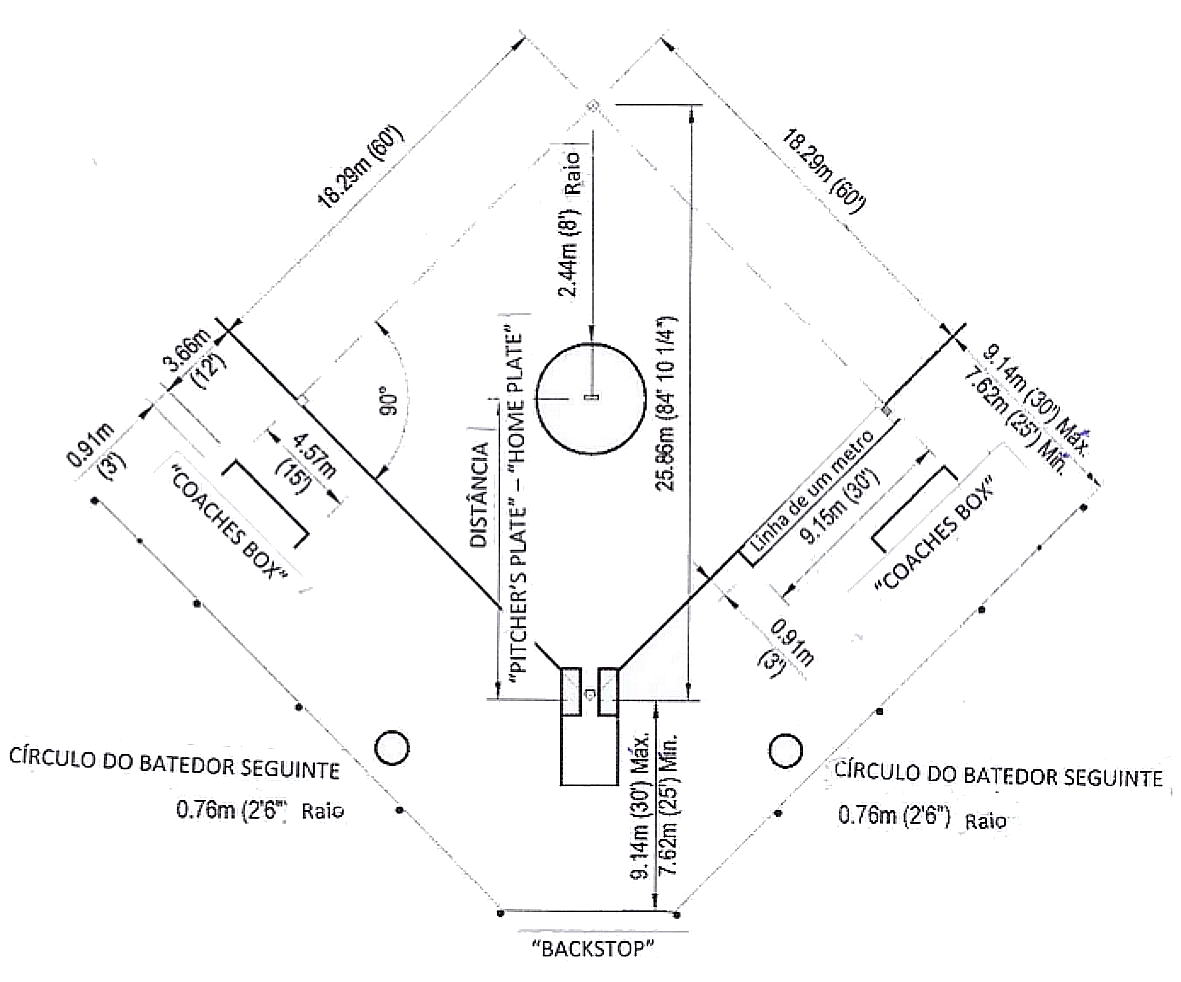
\includegraphics[width=.75\textwidth]{fig/campo02}\end{center}}

\section{DIMENSÕES OFICIAS DAS BASES}
{\begin{center}
		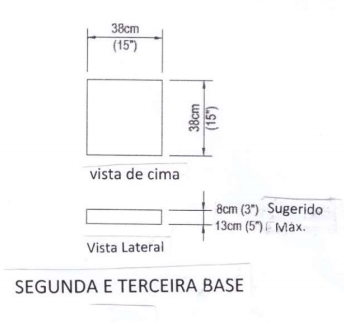
\includegraphics[width=.45\textwidth]{fig/base03}
		
\includegraphics[width=.45\textwidth]{fig/base01}
\end{center}}

\section{DIMENSÕES OFICIAIS DO “BATTER’S BOX” E “CATCHER’S BOX” }
{\begin{center}
		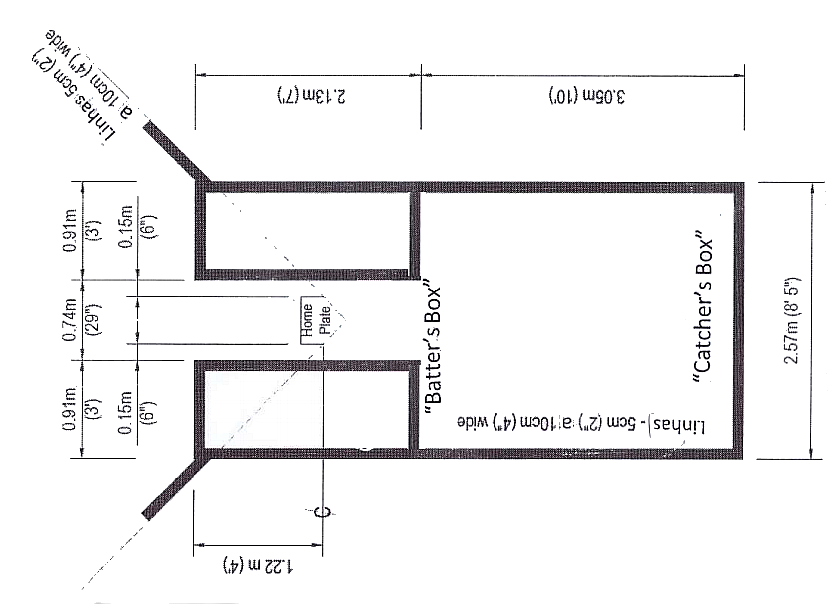
\includegraphics[width=.50\textwidth,angle=180]{fig/catcherbox}\end{center}}

\section[\textit{Home Plate} \Gls{pitcher's plate}]{DIMENSÕES OFICIAIS DO “HOME PLATE” E “PITCHER’S PLATE”}

{\begin{center}
		
\includegraphics[width=.45\textwidth]{fig/home}
		
\includegraphics[width=.45\textwidth]{fig/pitcher}
\end{center}}

\section{TABELA DE REFERÊNCIA RÁPIDA}

\resizebox{.95\textwidth}{!}{
	\begin{tabular}{p{40mm}p{160mm}}\footnotesize
		“BACKSTOP” E LINHAS LATERAIS (LINHA DE BOLA MORTA/CERCA LATERAL)& 
		O “backstop” (barreira situada atrás da área do “home plate”) e as linhas/cercas 
		laterais devem estar situadas a 7,62m (25 pés), no mínimo, e a 9,14m (30 pés), no 
		máximo, atrás das linhas de “foul”. A área entre as linhas de “foul” e o “backstop”, e 
		entre as linhas de “foul” e as linhas/ cercas laterais, tem de estar desobstruída. \\\hline
		BASES &
		Distâncias: “Home Plate” até primeira/terceira base: 18,29m (60 pés) da parte de trás 
		da placa até a parte de trás da base. “Home Plate” até segunda base: 25,86m (84 pés 
		10 1/4 polegadas) da parte de trás da placa até o meio da base. As bases devem ser 
		feitas de lona ou outro material apropriado, e devem estar firmemente fixadas em sua 
		posição. 
		
		Metade da Base Dupla (Primeira Base) é fixada em território “fair”, e é parte do 
		território “fair”, e a outra metade (de cor bem diferente e contrastante), em território 
		“foul”, e é parte do território “foul”. \\\hline
		“BATTER’S BOXES” &
		Um em cada parte do “home plate”. Devem medir 0,91m (3 pés) por 2,13m (7 pés). As 
		linhas internas do “batter’s box” devem estar a 15,20cm (6 polegadas) do “home 
		plate”. A linha dianteira do “box” deve estar a 1,22m (4 pés) na frente de uma linha 
		traçada através do centro do “home plate”. As linhas são consideradas dentro do 
		“batter’s box”. \\\hline
		“CATCHER’S BOX” &
		Medida: 3,05m (10 pés) de comprimento dos cantos externos traseiros dos “batter’s 
		boxes” e deve ter 2,57m (8 pés 5 polegadas) de largura. As linhas são consideradas 
		dentro do \gls{catcher's box}.\\\hline 
		“COACHES’ BOXES”& É aquela área atrás de uma linha de 4,57m (15 pés) traçada fora do “Diamond” 
		(campo). A linha é paralela à linha da primeira/terceira base, e está a 3,66m (12 pés) 
		dessas linhas, estendidas das bases em direção ao “home plate”. \\\hline
		TABELA DE DISTÂNCIAS &
		\begin{tabular}{l|c|c|c}
			\multicolumn{2}{c|}{CATEGORIA} &\parbox{30mm}{“H. PLATE”-“P. PLATE”}&\parbox{40mm}{ CERCAS DO CAMPO EXTERNO (mínimas)} \\\hline\hline
			\multirow{2}{*}{J\'unior fem.} 
			&16 anos e $<$ &12,19m (40 pés)&\multirow{3}{*}{ 67,06m (220 pés)} \\\cline{2-3}
			&19 anos e $<$& \multirow{2}{*}{13,11m (43 pés)}& \\\cline{1-2} 
			Feminino 	&			& & \\\hline
			\multirow{2}{*}{J\'unior masc.} 
			&16 anos e $<$&\multirow{3}{*}{14,02m (46 pés)} &\multirow{3}{*}{76,20m (250 pés)} \\\cline{2-2} 
			&19 anos e $<$& &   \\\cline{1-2} 
			Masculino 	&			& &   \\\hline
		\end{tabular}
		\\\hline
		“HOME PLATE” &
		Deve ter cinco lados. A borda voltada para o arremessador deve ter 43,20cm 
		(17polegadas) de largura. Os lados devem ser paralelos às linhas internas do “batter’s 
		box” e devem ter 21,60cm (8 $\frac{1}{2}$ polegadas) de comprimento. Os lados da ponta voltada 
		ao receptor devem ter 30,50cm (12 polegadas) de comprimento. \\\hline
		CAMPO INTERNO &
		“É aquela parte do campo, sem grama, que forma um arco a 18,29m (60 pés)s do 
		centro da borda dianteira do “pitcher’s plate”. LINHAS 
		Devem ter 50mm a 100mm (2 a 4 polegadas) de largura. \\\hline
		CÍRCULO DO BATEDOR PREVENIDO &
		É um círculo com 1,52m (5 pés), 0,76m (2 pés e 6 polegadas) de raio, localizado 
		próximo ao fim da área do “bench” ou “dugout” dos jogadores mais perto do “home 
		plate”. \\\hline
		LINHA DE UM METRO &
		Linha traçada paralelamente à linha de base, e a um metro (3 pés) dessa linha, 
		partindo de um ponto onde inicia a segunda metade da distância entre o “home plate” 
		e a primeira base. \\\hline
		CÍRCULO DO ARREMESSADOR &
		É um círculo de 4,88m (16 pés), com raio de 2,44m (8 pés), traçado do centro da borda 
		dianteira do “pitcher’s plate”. As linhas são consideradas dentro do círculo. \\\hline
		“PITCHER’S PLATE” &
		É feito de borracha e tem 61cm (24 polegadas) de comprimento e 15,2cm (6 
		polegadas) de largura. A parte superior da placa tem de estar no mesmo nível do solo. \\\hline
		ZONA DE ADVERTÊNCIA &
		Deve estar marcada a 3,66m (12 pés), no mínimo, e 4,57m (15 pés), no máximo, da 
		cerca do campo externo e/ou das cercas laterais. A marcação deve ser feita com 
		material (terra, cascalho) equivalente (mas diferente) ao da superfície do campo. O 
		material tem que ser distinguível do material da superfície do campo externo, e deve 
		chamar a atenção dos jogadores quando eles estão se aproximando da cerca. \\\hline
		
	\end{tabular}
}
\section{TRAÇANDO UM “DIAMOND” }

\begin{multicols}{2}
	Esta seção serve como um exemplo para traçar um campo (“diamond”) com distância 
	de 18,29m (60 pés) entre as bases e 14,02m (46 pés) entre o “home plate” e o 
	“pitcher’s plate”. 
	\begin{enumerate}[label= \arabic*)]
		\item  Para determinar a posição do “home plate”, trace uma linha na direção em que 
		deseja situar o campo. Fixe uma estaca no canto do “home plate” mais perto do 
		receptor. Amarre um cordão nessa estaca e dê nós ou marque a corda de outra forma 
		após medir 14,02m (46 pés), 18,29m (60 pés), 25,86m (84 pés e 10 $\frac{1}{4}$ polegadas) e 
		36,58m (120 pés). 
		\item  Coloque o cordão (sem esticar) ao longo da linha diretora e coloque uma estaca 
		onde marca 14,02m (46 pés). Esta será a linha de frente no meio do “pitcher’s plate”. 
		Ao longo da mesma linha, fixe uma estaca onde marca 25,86m (84 pés e 10 $\frac{1}{4}$ 
		polegadas). Este será o centro da segunda base. 
		\item  Coloque o ponto onde marca 36,58m (120 pés) no local determinado para o centro 
		da segunda base e, pegando o cordão no ponto onde marca 18,29m (60 pés), ande 
		para a direita da linha diretora até esticá-lo e pregue uma estaca no ponto onde marca 
		18,29m (60 pés) –este será o canto externo da primeira base, e o cordão, agora, 
		formará a linha entre a primeira e a segunda bases. 
		\item  Segurando, outra vez, o cordão no ponto onde marca 18,29m (60 pés), atravesse o 
		campo e, da mesma maneira, marque o canto externo da terceira base. O “home 
		plate”, a primeira base e a terceira base estão inteiramente na parte interna do campo 
		(“diamond”). 
		\item  Para conferir as medidas do campo (“diamond”), coloque a ponta da corda que 
		marca o “home plate” na estaca da primeira base, e o ponto onde marca 36,58m (120 
		pés), na terceira base. O ponto onde marca 18,29m (60 pés) deve, agora, coincidir com 
		os locais marcados para o “home plate” e a segunda base. 
		\item  Confira todas as distâncias com uma fita métrica metálica sempre que possível. ANEXO 2: 
	\end{enumerate}
\end{multicols}


\chapter{ESPECIFICAÇÕES DO \gls{bat} }

\section{\gls{bat} OFICIAL }\label{sec:bat}
\begin{multicols}{2}
	\begin{enumerate}[label= \arabic*)]
		\item  O \gls{bat} tem de ser feito com uma pe\c{c}a s\'o, com v\'arias pe\c{c}as juntadas 
		definitivamente, ou com duas pe\c{c}as troc\'aveis. 
		\item Quando o \gls{bat} \'e projetado para ser feito com componentes troc\'aveis, tem de levar em conta o seguinte crit\'erio: 
		\begin{enumerate}[label=\roman*.]
			\item os componentes acoplados devem ter um dispositivo de seguran\c{c}a especial para evitar que equipamento com combina\c{c}ões n\~ao aprovadas seja usado no campo; e 
			\item os “bats” confeccionados com combina\c{c}ões de componentes t\^em de seguir os padrões estabelecidos como se fossem um \gls{bat} feito com uma pe\c{c}a s\'o. Os componentes t\^em de seguir os padrões estabelecidos como se fossem partes de um \gls{bat} feito com uma pe\c{c}a s\'o. 
		\end{enumerate}
		\item  Um \gls{bat} pode ser feito com um peda\c{c}o de madeira de lei (madeira dura), ou com um bloco de madeira composto de dois ou mais peda\c{c}os de madeira colados entre si com um adesivo, de tal forma que a dire\c{c}\~ao das fibras de todas as pe\c{c}as seja paralela ao comprimento do "bat". 
		\item  Um “bat pode ser de metal, bambu, pl\'astico, grafite, carbono, magn\'esio, fibra de vidro, cer\^amica, ou qualquer outro material composto aprovado pela WBSC-SD ou ISF Equipment Standards Comission. 
		\item  Um \gls{bat} pode ser laminado, mas deve conter somente madeira ou adesivo, e ter um acabamento perfeito (quando pronto). 
		\item  A parte mais grossa do \gls{bat} (do início da parte cônica at\'e a ponta do \gls{bat}) deve ser redonda e lisa. 
		\item  N\~ao deve ter mais de 86,40cm (34 polegadas) de comprimento, nem pesar mais de 1077,00g (38 on\c{c}as). 
		\item  N\~ao deve ter mais de 5,70cm (2 1/4 polegadas) de di\^ametro em sua parte mais grossa. É permitida uma toler\^ancia de 0,80mm (1/32 polegada) devido \`a dilata\c{c}\~ao que pode haver no material. 
		\item  Um \gls{bat} n\~ao deve ter rebites expostos, pinos, bordas \'asperas ou afiadas, ou qualquer esp\'ecie de prendedor externo que possa apresentar algum risco. Um "bat" de metal n\~ao deve ter rebarbas nem rachaduras. 
		\item  Um \gls{bat} de metal n\~ao deve ter um cabo de madeira. 
		\item  Um \gls{bat} tem de ter uma empunhadura de seguran\c{c}a de corti\c{c}a, fita (fita pl\'astica n\~ao lisa) ou material composto. A empunhadura de seguran\c{c}a n\~ao deve ter menos de 25,40cm (10 polegadas) de comprimento e n\~ao deve se estender mais de 38,10cm (15 polegadas) da extremidade do cabo. É permitido aplicar resina, alcatr\~ao de pinho ou subst\^ancias em spray somente na empunhadura de seguran\c{c}a, para aumentar a sua efici\^encia. A fita aplicada a qualquer "bat" tem de ser em espiral contínua. N\~ao precisa ser uma camada s\'olida de fita. N\~ao deve exceder duas camadas. 
		\item  Se for de metal e n\~ao tiver sido feito em uma s\'o pe\c{c}a, com a extremidade da parte mais grossa fechada, dever\'a ter uma pe\c{c}a de borracha ou pl\'astico vinil, ou outro material aprovado pela WBSC-SD ou ISF Equipment Standards Commission, firmemente colocada nessa parte do "bat". 
		
		\begin{enumerate}[label=\roman*.]
			\item A tampa colocada na extremidade aberta da parte grossa do \gls{bat} tem de estar firme e permanentemente lacrada, para que ela n\~ao possa ser removida por qualquer pessoa, exceto o fabricante, sem danific\'a-la ou destrui-la. 
			\item O \gls{bat} n\~ao deve causar ruídos. Um \gls{bat} que causa ruídos ser\'a considerado um \gls{bat} ilegal. 
			\item O \gls{bat} n\~ao deve ter sinais de adultera\c{c}\~ao. Um \gls{bat} que mostra sinais de adultera\c{c}\~ao ser\'a considerado um \gls{bat} Adulterado. 
		\end{enumerate}
		\item  Um \gls{bat} tem que ter um dispositivo de seguran\c{c}a (sali\^encia arredondada na extremidade do cabo) de, no mínimo, 0,60cm (1/4 de polegada) ressaltando, a um \^angulo de 90 graus, do cabo, e n\~ao deve ter bordas afiadas. O dispositivo de seguran\c{c}a pode ser moldado, torneado, soldado e permanentemente fixo; pode ser coberto com fita. 
		
		\item  Um \gls{bat} que tenha a informa\c{c}\~ao “Bat Oficial Aprovado” ilegível, devido ao desgaste pelo uso, pode ainda ser utilizado se todos os outros aspectos estiverem de acordo com as regras, e desde que isso possa ser constatado com razo\'avel seguran\c{c}a. 
		\item  O peso, a distribui\c{c}\~ao do peso, ou o comprimento do "bat" t\^em de ser estabelecidos permanentemente por ocasi\~ao da fabrica\c{c}\~ao, e n\~ao podem ser modificados de maneira alguma depois disso, excetuando-se algo diferente que esteja especificamente previsto nesta Regra, ou haja uma especifica\c{c}\~ao aprovada pela WBSC-SD ou ISF Equipment Standards Commission. 
	\end{enumerate}
\end{multicols}

\section{\gls{bat} PARA FAZER AQUECIMENTO} 
\begin{multicols}{2}
	É um \gls{bat} (exceto um \gls{bat} oficial) que tem de ser feito com uma pe\c{c}a s\'o, e deve sujeitar-se aos requisitos exigidos aos dispositivos de seguran\c{c}a (empunhadura de seguran\c{c}a e sali\^encia arredondada na extremidade do cabo) do \gls{bat} oficial. Tem de estar marcado "warm-up", com letras de 3,20cm (1 1/4 polegada), na extremidade do 
	cilindro. A extremidade do cilindro tem que ter mais de 5,70cm (2 1/4 polegadas). 
	
\end{multicols}


\chapter{PADRÕES DE BOLA}
\label{ap:Bola}

\section{BOLA OFICIAL}


\begin{multicols}{2} 
	\begin{enumerate}[label= \arabic*)]
		\item  Tem que ser uma bola com formato regular, emendas lisas, pontos de costura não 
		salientes ou com superfície plana. 
		\item Tem que ter um núcleo central feito tanto de fibra longa de paina de primeira 
		qualidade, de uma mistura de cortiça e borracha, de uma mistura de poliuretano, 
		como de outros materiais aprovados pela WBSC-SD Equipment Standards Commission. 
		\item  Pode ser enrolada (manualmente ou a máquina) com fio trançado de boa qualidade 
		e coberta com cola de látex ou borracha. 
		\item Tem que ter uma cobertura costurada com fio encerado de algodão ou linho, colada 
		à bola mediante aplicação de substância aderente na face inferior (da cobertura), ou 
		uma cobertura moldada colada ao núcleo, ou uma cobertura integralmente moldada 
		com o núcleo. As peças moldadas devem ter uma reprodução autêntica da costura 
		aprovada pela WBSC-SD Equipment Standards Commission. 
		\item  Tem que ter uma cobertura da melhor qualidade, feita de couro de cavalo ou vaca 
		curtido em cromo Nº 1, ou de material sintético ou outros materiais aprovados pela 
		WBSC-SD Equipment Standards Commission. 
	\end{enumerate}
\end{multicols}

\section{DIMENSÕES E ESPECIFICAÇÕES}
\begin{multicols}{2} 
	\begin{enumerate}[label= \arabic*)]
		\item  A bola de 30,50cm (12 polegadas), pronta, deve ter entre 30,20cm (11 7/8 
		polegadas) e 30,80cm (12 1/8 polegadas) de circunferência, e deve pesar entre 
		178,00g (6 $\frac{1}{4}$ onças) e 198,40g (7 onças). O tipo “costura plana” deve ter, no mínimo, 
		88 pontos em cada cobertura, costurados pelo método de duas agulhas. 
		\item  A bola pronta deve ter um coeficiente de restituição e um padrão de compressão, 
		que serão determinados e instituídos pela WBSC-SD Equipment Standards 
		Commission. 
		\item  COR significa Coeficiente de Restituição de uma bola quando medido pelo método 
		de teste para medir o Coeficiente de Restituição de bolas da ASTM (American Society 
		for Testing and Materials). 
		\item  A bola de 30,50cm (12 polegadas), com costura branca ou vermelha ou cobertura 
		amarela com um COR de .47 ou menos, deve ser usada em jogos de Campeonato da 
		WBSC-SD, nas seguintes categorias: Adultos (Masculino e Feminino), Júnior (Masculino 
		e Feminino). As bolas devem ter a logomarca da WBSC-SD. 
		\item  Em bolas usadas em Jogos de Campeonato da WBSC-SD, a força de carga exigida 
		para comprimir a bola 0,64cm (0,25 polegadas) não precisa exceder 170,10kg (375 libras) quando tais bolas são testadas de acordo com o método de provas para medir compressão-deslocamento de bolas de softbol da ASTM, método esse aprovado pela WBSC-SD Equipment Standards Commission. 
	\end{enumerate}
\end{multicols}
Abaixo, estão relacionados os padrões estabelecidos para cada bola: 

\resizebox{\textwidth}{!}{\begin{tabular}{*{8}{c}}
		Bola& Cor da bola &Cor da linha &Tam. Mín.& Tam. Max.& Peso mín.& Peso Max. & Marcação \\\hline\hline
		30,50cm& Branca ou& Costura Bca.& 30,20cm& 30,80cm& 178,00g &198,40g&\multirow{2}{*}{LOGO da WBSC-D}\\\cline{1-7}
		(12”)& Tom. Amar &ou Verm.& (11-7/8”)& (12-1/8”)& (6 $\frac{1}{4}$ onças)&(7onças) &
		\\\hline
\end{tabular}}


\chapter{ESPECIFICAÇÕES DA LUVA} \label{chap:Luva}

ESPECIFICAÇÕES DAS DIMENSÕES: 

\begin{center}
	
\includegraphics[width=.5\textwidth]{fig/Luva}
	
	
	\begin{tabular}{c |p{90mm}|r|r}
		&&cm& polegadas \\\hline\hline
		A& Largura da palma parte superior &20,30& 8  \\\hline
		B& Largura da palma parte inferior &21,60& 8 $\frac{1}{2}$ \\\hline 
		C& Abertura da parte superior do trançado &12,70 &5  \\\hline
		D& Abertura da parte inferior do trançado &11,50 &4 $\frac{1}{2}$  e\\\hline
		E& Topo à base do trançado &18,40& 7 $\frac{1}{4}$  \\\hline
		F& Costura da forquilha do primeiro dedo &19,00 &7 $\frac{1}{2}$  \\\hline
		G& Costura da forquilha do polegar &19,00& 7 $\frac{1}{2}$ \\\hline 
		H& Costura da forquilha &44,50& 17 $\frac{1}{2}$  \\\hline
		I& Topo do polegar à borda inferior &23,50 &9 $\frac{1}{4}$  \\\hline
		J& Topo do primeiro dedo à borda inferior &35,60 &14  \\\hline
		K& Topo do segundo dedo à borda inferior &33,70 &13 $\frac{1}{4}$  \\\hline
		L& Topo do terceiro dedo à borda inferior& 31,10& 12 $\frac{1}{4}$  \\\hline
		M& Topo do quarto dedo à borda inferior& 27,90 &11  \\\hline
	\end{tabular}  
\end{center}


\chapter{ÁRBITROS}



\section{INFORMAÇÕES GERAIS PARA ÁRBITROS }
\begin{multicols}{2}  
	\begin{enumerate}[label=\alph*)]
		\item O árbitro não deve ser um membro de nenhuma das equipes. Exemplos: jogador, 
		"coach", técnico, dirigente, anotador ou patrocinador. 
		
		\item  O árbitro deve estar seguro quanto à data, ao horário e ao local do jogo, e deve 
		chegar ao campo de jogo com antecedência de 20 a 30 minutos, iniciar o jogo 
		pontualmente e deixar o campo depois de encerrá-lo. 
		
		\item  O árbitro (masculino e feminino) tem de usar: 
		\begin{enumerate}[label= \arabic*)]
			\item  Uma camisa azul-claro, com mangas longas ou curtas. 
			\item  Meias azul-marinho escuro. 
			\item  Calças azul-marinho escuro. 
			\item  Boné azul-marinho escuro, com a marca WBSC (em letras brancas decoradas com 
			contornos azuis) pregada na frente. 
			\item  Bolsa para bolas azul-marinho escuro (somente árbitro de "home"). 
			\item  Jaqueta e/ou pulôver azul-marinho escuro. 
			\item  Sapatos e cinto pretos. 
			\item  Uma camiseta branca, que deve ser usada por baixo da camisa azul-claro. 
		\end{enumerate}
		
		
		\item  Árbitros não devem usar joias expostas que possam oferecer risco. 
		
		EXCETO braceletes e/ou colares com fins medicinais. 
		
		\item  O árbitro de "home", na modalidade Arremesso Rápido, tem de usar uma máscara para rosto preta, com estofamento preto ou bege, um protetor de garganta preto, um protetor de tórax e caneleiras que protejam também os joelhos. (Pode ser usada uma máscara que já vem dotada de um protetor de garganta na parte inferior da armação.) 
		
		\item  Os árbitros devem apresentar-se aos capitães, técnicos e anotadores. 
		
		\item  Os árbitros devem inspecionar as delimitações do campo de jogo, o equipamento etc. e esclarecer todas as regras de campo para ambas as equipes e seus "coaches". 
		
		\item  Cada árbitro tem o poder de tomar decisões sobre as infrações cometidas a qualquer momento durante o desenrolar da partida, ou enquanto ela está paralisada, até o jogo ser encerrado.
		\item Nenhum árbitro tem autoridade para desprezar ou questionar as decisões tomadas por outro árbitro dentro dos limites de seus respectivos deveres, conforme está especificado nestas regras. 
		
		\item  Um árbitro pode consultar seu companheiro a qualquer momento. Contudo, a decisão final deve ser do árbitro que, mesmo tendo autoridade exclusiva para decidir, recorreu à opinião de outro árbitro. 
		
		\item  Para definir suas respectivas obrigações, o árbitro que julga as bolas arremessadas ("ball" ou "strike") será designado como o "Árbitro de Home", e o árbitro que julga as decisões nas bases, como o "Árbitro de Base". 
		
		\item  O árbitro de "home" e o árbitro de base devem ter a mesma autoridade para: 
		\begin{enumerate}[label= \arabic*)]
			\item Declarar declarado “OUT” um corredor que sai da base antecipadamente. 
			\item Declarar "TIME" para paralisar o jogo. 
			\item Remover, ou expulsar do jogo, um jogador, "coach" ou técnico, por violação de regras. 
			\item Declarar todos os Arremessos Ilegais. 
			\item Determinar e declarar um “Infield Fly”. \textbf{Quando parecer evidente que uma bola batida será um “Infield Fly”, o árbitro deverá declarar, imediatamente, “INFIELD FLY” SE FOR “FAIR”, OBATEDOR É “OUT”, para beneficiar os corredores}.
		\end{enumerate}
		\item  O árbitro deve declarar declarado “OUT” o batedor, batedor-corredor ou corredor, sem esperar por uma apelação para tal decisão, em todos os casos em que esse jogador é declarado “OUT” de acordo com estas regras. 
		
		\item  A menos que haja uma apelação, o árbitro não deve declarar declarado “OUT” um jogador, ou penalizá-lo, por não ter tocado uma base; por ter deixado uma base antecipadamente numa bola \gls{fly} pega no ar; por ter batido fora de ordem; por ter entrado no jogo como substituto sem ser anunciado ao árbitro; por ter reingressado ilegalmente; por ter entrado no jogo como Jogador de Emergência, ou por ter retornado ao jogo após ter sido removido de acordo com a Regra de Jogador de Emergência, sem comunicação ao árbitro; por ter mudado de posições nas bases com outro corredor; ou por ter tentado ir à segunda base depois de chegar à primeira base, conforme está estabelecido nestas regras. 
		
		\item  Os árbitros não devem penalizar uma equipe por infração de uma regra quando a imposição da penalidade pode resultar em vantagem à equipe infratora. 
		
		\item  A inobservância, pelos árbitros, das instruções contidas no Anexo 5 não é motivo para protesto. Estas instruções são normas de procedimento para árbitros. 
	\end{enumerate}
\end{multicols}
\section{SINAIS}
\begin{multicols}{2}  
	\begin{enumerate}[label=\alph*)]
		\item Para indicar que a partida deve começar, ou ser retomada, o árbitro deve declarar "PLAY BALL" e, ao mesmo tempo, sinalizar para o arremessador efetuar o arremesso. 
		
		\item  Para indicar um “STRIKE”, o árbitro deve levantar a mão direita acima do ombro (dobrar o cotovelo, de modo que forme um ângulo de 90 graus) e, ao mesmo tempo, declarar “STRIKE” com voz clara e firme. 
		
		\item  Para indicar um "BALL", não deve ser usado sinal algum com o braço. 
		
		\item  Para indicar a CONTAGEM de "balls" e "strikes", o árbitro deve declarar a quantidade de "balls" primeiro. 
		
		\item  Para indicar um "FOUL", o árbitro deve declarar "FOUL BALL" e estender ambos os braços, verticalmente, acima da cabeça. 
		
		\item  Para indicar uma bola "FAIR", o árbitro deve estender um braço na direção do centro do campo, agitando-o para a frente e para trás, imitando um movimento de bombeamento. 
		
		\item  Para indicar que um batedor ou corredor é “OUT”, o árbitro deve levantar a mão direita, com o punho cerrado, acima do ombro direito. 
		
		\item  Para indicar que um jogador é "SAFE", o árbitro deve estender ambos os braços, horizontalmente, para os lados do corpo, com as palmas das mãos viradas para o solo. 
		
		\item  Para indicar a paralisação da partida, o árbitro deve declarar "TIME" e, ao mesmo tempo, estender ambos os braços acima da cabeça. Os outros árbitros devem confirmar a paralisação da partida, imediatamente, fazendo o mesmo gesto. 
		
		\item  Para indicar uma BOLA MORTA DEMORADA (“DELAYED DEAD BALL”), o árbitro deve estender o braço esquerdo, horizontalmente, mantendo o punho cerrado. 
		
		\item  Para indicar um "TRAPPED BALL", o árbitro deve estender ambos os braços, horizontalmente, para os lados do corpo, com as palmas das mãos viradas para o solo. 
		
		\item  Para indicar que o batedor-corredor (ou corredor) tem direito a duas bases (\gls{ground rule double}), o árbitro deve estender a mão direita acima da cabeça e, ao mesmo tempo, indicar com dois dedos o número de bases concedidas. 
		
		\item  Para indicar um \textit{home run}, o árbitro deve estender a mão direita com o punho cerrado, acima da cabeça, e fazer um movimento circular em sentido horário. 
		
		\item  Para indicar um "INFIELD FLY", o árbitro deve declarar "INFIELD FLY" SE FOR "FAIR", O BATEDOR É “OUT”. O árbitro deve estender um braço acima da cabeça. 
		
		\item Para indicar que o arremessador não deve efetuar o arremesso ("NOT TO PITCH"), o árbitro deve levantar uma mão com a palma da mão virada para o arremessador. Deve ser declarado “NO PITCH” (arremesso nulo) se o arremessador efetua o arremesso enquanto o árbitro está com sua mão na posição mencionada. 
	\end{enumerate}
\end{multicols}

\chapter{ANOTAÇÃO }

\section{\textit{BOX SCORE}}

\footnote{N.T.: REGISTRO DE DADOS }
\begin{multicols}{2} 
	
	\begin{enumerate}[label=\alph*)]
		\item O nome de cada jogador e a posição, ou posições, a ser(em) ocupada(s) devem ser relacionadas na ordem em que ele bateu, ou teria batido, a menos que o jogador seja substituído legalmente, expulso ou removido do jogo, ou o jogo termine antes de sua vez de bater.
		
		Quaisquer dados estatísticos acumulados pelo Jogador de Emergência enquanto estava no jogo são creditados a esse jogador, mesmo que ele seja um substituto constante da lista que, eventualmente, não entre no jogo para substituir outro jogador. 
	\end{enumerate}
	\textbf{Quaisquer dados estatísticos acumulados por um Corredor Temporário devem ser creditados ao jogador por quem ele está correndo.} 
	\begin{enumerate}[label= \arabic*)]
		\item  O Jogador Designado (JD) é opcional, mas, se vai utilizar um, seu nome tem de ser anunciado antes do início do jogo e estar relacionado no Formulário de Anotações, na ordem correta em que vai atuar como batedor. Serão relacionados dez nomes, e o décimo nome será o do “JOGADOR FLEX” por quem o JD está batendo. 
		\begin{enumerate}[label=(\alph*)]
			\item Os dados referentes à atuação de cada jogador, na ofensiva e na defensiva, têm de 
			estar tabulados. 
		\end{enumerate}
		\item A primeira coluna deve indicar o número de vezes que cada jogador atua como batedor ("at bat"), mas não deve ser imputado um "at bat" contra o jogador quando esse batedor 
		\begin{enumerate}[label= (\alph*)]
			\item Bate um \gls{fly de sacrificio} que ocasiona a marcação de um ponto. 
			\item É autorizado a ‘andar’ (“walk”, “base on balls”). 
			\item É autorizado a ir à primeira base por ter sofrido Obstrução. 
			\item Executa um "bunt" de sacrifício. 
			\item É atingido por uma bola arremessada (\textit{hit by pitch}). 
		\end{enumerate}
		\item A segunda coluna deve indicar a quantidade de pontos anotados por cada jogador. 
		\item A terceira coluna deve indicar a quantidade de \textit{base hits}\footnote{N.T.: batidas indefensáveis}
		batidos por cada jogador. Uma batida indefensável é aquela que permite que o 
		batedor chegue a salvo ("safe") a uma base. 
		\begin{enumerate}[label= (\alph*)]
			\item Quando um batedor-corredor chega a salvo ("safe") à primeira base, ou a qualquer base subsequente, numa bola "fair" que fica no campo, transpõe a cerca, ou atinge a cerca antes de ser tocada por um defensor. 
			\item Quando um batedor-corredor chega a salvo ("safe") à primeira base numa bola “fair” –muito forte, ou muito lenta, ou que dá um salto incomum– impossível de ser defendida por um defensor, com um esforço normal, a tempo de eliminar esse batedor-corredor. 
			\item Quando uma bola "fair" que não tenha tido contato com um defensor se torna "morta" por ter tocado o corpo ou a roupa de um corredor ou árbitro. 
			\item Quando o defensor tenta, sem sucesso, eliminar um corredor precedente e, na opinião do anotador, o batedor-corredor não teria sido declarado “OUT” na primeira base com uma defesa perfeita. 
			\item  Quando o batedor termina o jogo com uma batida indefensável que empurra os pontos necessários para colocar a sua equipe em vantagem no placar, a ele deve ser creditado somente um "base hit" de tantas bases quantas tiver avançado o corredor que anotou o ponto da vitória, com a condição de que ele (o batedor) avance o mesmo número de bases. 
		\end{enumerate}
		
		EXCEÇÃO: Quando o batedor termina o jogo com um \textit{home run} batido para fora do campo, ele deve ser creditado com um \textit{home run}, e todos os corredores, incluindo ele, devem ser autorizados a anotar ponto. 
		
		\item A quarta coluna deve indicar a quantidade de adversários declarado “OUT”s por 
		cada jogador ("put out"). 
		\begin{enumerate}[label= (\alph*)]
			\item Um "put out" é creditado a um defensor cada vez que ele: 
			\begin{enumerate}[label= (\arabic*)]
				\item Pega uma bola batida para o ar (\gls{fly}) ou uma batida em linha reta ("line drive"). 
				\item Pega uma bola lançada que elimina um batedor ou corredor. 
				\item Toca um corredor com a bola quando esse corredor está fora da base na qual tem o direito de permanecer. 
				\item Está mais perto da bola quando um corredor é declarado “OUT” por ter sido 
				atingido por uma bola "fair" ou por ter estorvado um defensor. 
				\item Está mais perto do jogador substituto não anunciado, que é declarado “OUT” de 
				acordo com a Regra 3.2.8. 
				\item Está mais perto de um corredor que é declarado “OUT” por correr fora do caminho da base. 
			\end{enumerate}		
			\item Um "put out" é creditado ao receptor 
			\begin{enumerate}[label= (\arabic*)]
				\item Quando é declarado um terceiro "strike". 
				\item Quando o batedor não bate na ordem correta. 
				\item Quando o batedor interfere na ação do receptor. 
				\item Quando o batedor é declarado “OUT” por ter batido ilegalmente. 
				\item  Quando o batedor é declarado “OUT” em razão de uma tentativa de “bunt” depois de dois “strikes” ter resultado em “foul ball”. 
				\item Quando o batedor é declarado “OUT” por usar um "bat" ilegal ou Adulterado. 
				\item Quando o batedor é declarado “OUT” por ter mudado de um "batter's box" a outro. 
			\end{enumerate}	
		\end{enumerate}
		\item A quinta coluna deve indicar a quantidade de assistências (“assists”) dadas nas 
		eliminações por cada defensor. Deve ser creditada uma assistência 
		\begin{enumerate}[label= (\alph*)]
			\item A cada jogador que maneja a bola em qualquer série de jogadas que resulte na 		eliminação do corredor. Deve ser atribuída somente uma assistência –não mais–a um 		jogador que maneja a bola em qualquer eliminação. Um jogador que tenha auxiliado 		numa Jogada de Perseguição ("Run-Down Play") ou outra jogada do gênero pode ser 		creditado com um “assist” e um "put out". 
			\item A cada jogador que maneja, ou lança, a bola de tal maneira que poderia ter 		contribuído na eliminação de um corredor se não ocorresse um erro subsequente de 		um companheiro de equipe. 			
			\item A cada jogador que, desviando uma bola batida, ajuda na eliminação de um 
			corredor. 
			\item A cada jogador que maneja a bola numa jogada que resulte na eliminação de um 
			corredor, por Interferência, ou por correr fora da linha de base. 
		\end{enumerate}
		
		\item A sexta coluna deve indicar a quantidade de erros cometidos por cada jogador. Erros 
		são registrados nas seguintes situações: 
		\begin{enumerate}[label= (\alph*)]
			\item A cada jogador que executa uma má jogada ("misplay") que prolongue o turno do 
			batedor, ou a vida de um corredor que está ocupando alguma base. 
			\item Ao defensor que deixa de tocar a base após receber a bola para eliminar o 
			corredor, numa Jogada Forçada ou quando esse corredor é obrigado a retornar à base. 
			\item Ao receptor, se um batedor é autorizado a ir à primeira base por Obstrução. 
			\item Ao defensor que deixa de completar uma Jogada Dupla ("Double Play") por ter 
			derrubado a bola. 
			\item Ao defensor, se um corredor avança uma base em razão da falha desse defensor 
			em parar ou tentar parar uma bola lançada corretamente a uma base, contanto que tenha havido motivo para o lançamento. Quando mais de um jogador poderia ter 
			recebido o lançamento, o anotador tem de determinar a quem atribuir o erro. 
		\end{enumerate}
	\end{enumerate}
\end{multicols}

\section[Bat Indefens\'aveis]{NÃO DEVEM SER REGISTRADOS \textit{base hits} (BATIDAS INDEFENSÁVEIS) }
\begin{multicols}{2} 
	Não deve ser anotado um "base hit" nos seguintes casos: 
	
	\begin{enumerate}[label=\alph*)]
		\item Quando um corredor é declarado “OUT” em Jogada Forçada, ou teria sido declarado 
		“OUT” em Jogada Forçada se um defensor não tivesse cometido erro. 
		
		\item  Quando um jogador que pega uma bola batida elimina um corredor precedente com 
		um esforço normal. 
		
		\item  Quando um defensor tenta, mas não consegue eliminar um corredor precedente e, 
		na opinião do anotador, o batedor-corredor poderia ter sido declarado “OUT” na 
		primeira base. 
		
		\item  Quando um batedor-corredor chega a salvo ("safe") à primeira base porque um 
		corredor precedente é declarado “OUT” por ter interferido numa bola batida ou na 
		ação de um jogador da defensiva. 
	\end{enumerate}
	EXCEÇÃO: Se, na opinião do anotador, o batedor teria chegado a salvo ("safe") à 
	primeira base se não tivesse ocorrido a Interferência, a ele deve ser creditado um "safe 
	hit" (batida por meio da qual o batedor-corredor chega a salvo à primeira base). 
\end{multicols}

\section{FLY DE SACRIFÍCIO }
\begin{multicols}{2}
	É anotado um \gls{fly de sacrificio} quando, com menos de dois “outs”, 
	
	\begin{enumerate}[label=\alph*)]
		\item O batedor empurra um ponto com um “fly” que é pego no ar; ou 
		
		\item  Um corredor anota ponto depois que um defensor do campo externo (ou um 
		defensor do campo interno que tenha corrido para o campo externo) derruba um \gls{fly} 
		ou "line drive" após ter tocado a bola, e, na opinião do anotador, esse corredor 
		poderia ter pisado o “home plate”, mesmo que o defensor a tivesse pego no ar. 
	\end{enumerate}
\end{multicols}
\section{PONTOS EMPURRADOS (\textit{run batted in}) }
\begin{multicols}{2} 
	São os pontos anotados por meio de: 
	
	\begin{enumerate}[label=\alph*)]
		\item Um \textit{safe hit}. 
		
		\item  Um "bunt" de sacrifício ou um \textit{slap hit} (SOMENTE AR), ou um \gls{fly de sacrificio} (AR e AL). 
		
		\item  Um \textit{foul fly} pego no ar.
		\item Um "infield put out" (eliminação feita no campo interno) ou "fielder's choice" 
		(opção feita por um defensor na hora de executar uma jogada). 
		
		\item  Ocorrências que forçam um corredor a avançar para "home": por causa de 
		Obstrução, porque o batedor é atingido por uma bola arremessada (\textit{hit by pitch}), ou 
		em razão da concessão de uma base por “balls”. 
		
		\item  Um \textit{home run} e todos os pontos anotados como decorrência desse \textit{home run}. 
	\end{enumerate}
\end{multicols}
\section{ARREMESSADOR CREDITADO COM UMA VITÓRIA }
\begin{multicols}{2} 
	Um arremessador será creditado com uma vitória, nas seguintes situações: 
	
	\begin{enumerate}[label=\alph*)]
		\item Quando, na condição de arremessador abridor, tiver arremessado pelo menos 
		quatro “innings”, e sua equipe, que estava ganhando no momento em que foi 
		substituído, permanecer liderando o placar pelo resto do jogo. 
		
		\item  Quando, numa partida encerrada depois de jogados cinco “innings”, o arremessador 
		abridor tiver arremessado pelo menos três “innings”, e sua equipe tiver anotado mais 
		pontos do que a outra no momento em que a partida é dada por terminada. 
	\end{enumerate}
\end{multicols}
\section{ARREMESSADOR DEBITADO COM UMA DERROTA }
\begin{multicols}{2} 
	Um arremessador será debitado com uma derrota, independentemente do número de 
	“innings” que tenha arremessado, se for substituído quando sua equipe está perdendo 
	e, depois disso, ela não consegue empatar ou tomar a dianteira no placar. 
\end{multicols}
\section{RESUMO DO JOGO }
\begin{multicols}{2} 
	O resumo deve relacionar os seguintes itens, nesta ordem: 
	
	\begin{enumerate}[label=\alph*)]
		\item A quantidade de pontos por "inning" e a contagem final. 
		
		\item  Os pontos empurrados (\textit{run batted in}) e quem os empurrou. 
		
		\item  “Hits" de duas bases ("two-base hits") e quem os bateu. 
		
		\item  "Hits" de três bases ("three-base hits") e quem os bateu. 
		
		\item  "Home runs" e quem os bateu. 
		
		\item  \Gls{fly de sacrificio} (\textit{sacrifice flies}) e quem os bateu. 
		
		\item  Jogadas Duplas ("Double Plays") e os jogadores que delas participaram. 
		
		\item  Jogadas Triplas ("Triple Plays") e os jogadores que delas participaram. 
		
		\item  Quantidade de "walks" (“base on balls”) concedidos por cada arremessador.
		\item Quantidade de batedores declarado “OUT”s por "strike" ("strikeouts") por cada 
		arremessador. 
		
		\item  Quantidade de "hits" e pontos permitidos por cada arremessador. 
		
		\item  O nome do arremessador vencedor. 
		
		\item  O nome do arremessador perdedor. 
		
		\item  O tempo de duração do jogo. 
		
		\item  Os nomes dos árbitros e anotadores. 
		
		\item  Bases roubadas ("stolen bases") e por quem. 
		
		\item  “Bunts" de sacrifício. 
		
		\item  Os nomes dos batedores atingidos por uma bola arremessada e dos arremessadores 
		que os atingiram. 
		
		\item  A quantidade de “wild pitches” feitos por cada arremessador. 
		
		\item  A quantidade de "passed balls" feitos por cada receptor. 
	\end{enumerate}
\end{multicols}
\section{BASES ROUBADAS} 
\begin{multicols}{2} 
	(SOMENTE AR) Deve-se creditar uma base roubada ("stolen base") a um corredor, 
	sempre que ele avança uma base sem a ajuda de um "hit", um "put out", um erro, uma 
	eliminação forçada, um "fielder's choice", um "passed ball", um "wild pitch" ou um 
	arremesso ilegal. Isso inclui um batedor-corredor que avança à segunda base numa 
	base por “balls” concedida. 
\end{multicols}

\section{DADOS DE JOGOS CONFISCADOS ("FORFEITED GAMES")} 
\begin{multicols}{2} 
	Todos os dados de um jogo confiscado devem ser incluídos nas anotações oficiais, 
	exceto aquele registro de arremessador ganhador/perdedor. 
\end{multicols}


\chapter{NOMENCLATURA DAS ATLETAS NAS POSIÇÕES DO CAMPO}

\begin{figure}[!ht]
	\caption{Posicionamento das atletas}
	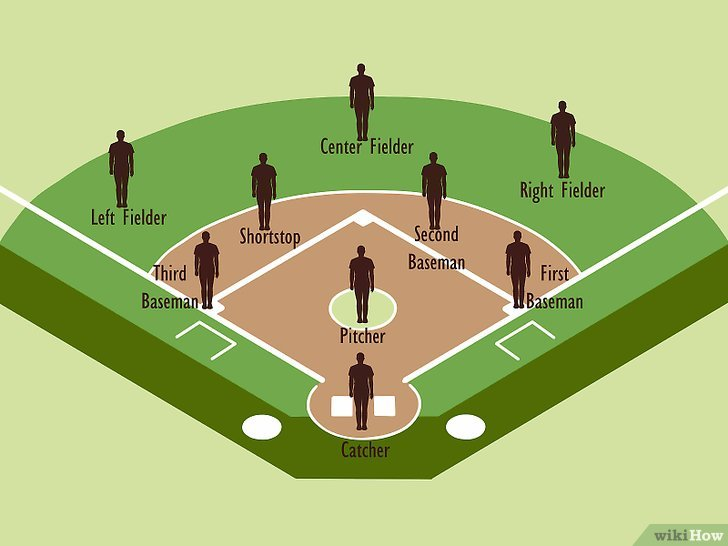
\includegraphics[width=.8\textwidth]{fig/v4-728px-Play-Softball-Step-4-Version-3}
	
	\par Fonte:\url{https://pt.wikihow.com/Jogar-Softbol}
\end{figure}


\chapter{JAPONGLÊS}



\begin{table}[!ht]
	\begin{center}
		\begin{tabular}{lll}
			Japonglês & Inglês      & Português               \\\hline\hline
			Bora      & Ball        & Bola                    \\\hline
			Globo     & Glove       & Luva                    \\\hline
			Polo      & Pole        & Poste                   \\\hline
			Quiátia   & Catcher     & Receptor                \\\hline
			Fasto     & First       & Primeira base           \\\hline
			Secando   & Second      & Segunda base            \\\hline
			Sado      & Third       & Terceira base           \\\hline
			Shoto     & Shortstop   & Interbase               \\\hline
			Gaiá      & Outfielder  & Jardineiro              \\\hline
			Naiá      & Infielder   & Jogador da linha        \\\hline
			Homoran   & Home run    & Rebatida quádrupla      \\\hline
			Guetso    & Get two     & Eliminação dupla        \\\hline
			Tsuberi   & Dive        & Mergulho                \\\hline
			Cabo      & Curveball   & Bola curva              \\\hline
			Naco      & Knuckleball & Arremesso com as juntas \\\hline
			Chenjapo  & Change-up   & Bola lenta              \\\hline
			Furai     & Fly         & Bola alta               \\\hline
			Goro      & Ground      & Bola para o chão       \\\hline
			Yakyuu    & Baseball	& Basebol
		\end{tabular}
		
		\vspace{5mm}
		\footnotesize{Fonte: https://esporte.uol.com.br/olimpiadas/ultimas/2004/07/21/ult2250u4.jhtm}
	\end{center}
\end{table}

\newpage

\begin{table}[!ht]
	\begin{center}
		
		
		\begin{tabular}{lll}
			\begin{CJK}{UTF8}{min}日本語\end{CJK} & japon\^es& Ingl\^es\\\hline\hline
			\begin{CJK}{UTF8}{min}クローザー \end{CJK} &kuroozaa                     & closer              \\\hline
			\begin{CJK}{UTF8}{min}セーブ \end{CJK} &seebu                          & save                \\\hline
			\begin{CJK}{UTF8}{min}ホームラン, 本塁打 \end{CJK} &hoomuran or hon-rui da  & home run            \\\hline
			\begin{CJK}{UTF8}{min}一塁 \end{CJK} &ichi-rui                        & first base          \\\hline
			\begin{CJK}{UTF8}{min}一塁手 \end{CJK} &ichi-rui shu                   & first baseman       \\\hline
			\begin{CJK}{UTF8}{min}三塁 \end{CJK} &san-rui                         & third base          \\\hline
			\begin{CJK}{UTF8}{min}	三塁手 \end{CJK} &san-rui shu                    & third baseman       \\\hline
			\begin{CJK}{UTF8}{min}三塁打 \end{CJK} &san-rui da                     & triple              \\\hline
			\begin{CJK}{UTF8}{min}三振 \end{CJK} &sanshin                         & strikeout           \\\hline
			\begin{CJK}{UTF8}{min}中堅, センター \end{CJK} &chuuken or sentaa         & center field        \\\hline
			\begin{CJK}{UTF8}{min}中堅手 \end{CJK} &chuukenshu                     & center fielder      \\\hline
			\begin{CJK}{UTF8}{min}二塁 \end{CJK} &ni-rui                          & second base         \\\hline
			\begin{CJK}{UTF8}{min}二塁手 \end{CJK} &ni-rui shu                     & second baseman      \\\hline
			\begin{CJK}{UTF8}{min}二塁打 \end{CJK} &ni-rui da                      & double              \\\hline
			\begin{CJK}{UTF8}{min}先発投手 \end{CJK} &senpatsu-toushu               & starting pitcher    \\\hline
			\begin{CJK}{UTF8}{min}内野 \end{CJK} &naiya                           & infield             \\\hline
			\begin{CJK}{UTF8}{min}出塁率 \end{CJK} &shutsuruiritsu                 & on-base percentage  \\\hline
			\begin{CJK}{UTF8}{min}勝利 \end{CJK} &shouri                          & win                 \\\hline
			\begin{CJK}{UTF8}{min}右翼 , ライト \end{CJK} &uyoku or raito            & right field         \\\hline
			\begin{CJK}{UTF8}{min}右翼手 \end{CJK} &uyokushu                       & right fielder       \\\hline
			\begin{CJK}{UTF8}{min}四球, フォアボール \end{CJK} &shikyuu or foa-booru    & walk                \\\hline
			\begin{CJK}{UTF8}{min}外野 \end{CJK} &gaiya                           & outfield            \\\hline
			\begin{CJK}{UTF8}{min}安打 \end{CJK} &anda                            & hit                 \\\hline
			\begin{CJK}{UTF8}{min}審判 \end{CJK} &shinpan                         & umpire              \\\hline
			\begin{CJK}{UTF8}{min}左翼,  レフト \end{CJK} &sayoku or refuto          & left field          \\\hline
			\begin{CJK}{UTF8}{min}左翼手 \end{CJK} &sayokushu                      & left fielder        \\\hline
			\begin{CJK}{UTF8}{min}得点 \end{CJK} &tokuten                         & run                 \\\hline
			\begin{CJK}{UTF8}{min}打席 \end{CJK} &daseki                          & at bat              \\\hline
			\begin{CJK}{UTF8}{min}打点 \end{CJK} &daten                           & runs batted in      \\\hline
			\begin{CJK}{UTF8}{min}打率 \end{CJK} &daritsu                         & batting average     \\\hline
			\begin{CJK}{UTF8}{min}投手 \end{CJK} &toushu                          & pitcher             \\\hline
			\begin{CJK}{UTF8}{min}指名打者 \end{CJK} &shimei-dasha                  & designated hitter   \\\hline
			\begin{CJK}{UTF8}{min}捕手 \end{CJK} &hoshu                           & catcher             \\\hline
			\begin{CJK}{UTF8}{min}救援投手 \end{CJK} &kyuuen-toushu                 & relief pitcher      \\\hline
			\begin{CJK}{UTF8}{min}敗戦 \end{CJK} &haisen                          & loss                \\\hline
			\begin{CJK}{UTF8}{min}本塁, ホーム \end{CJK} &hon-rui or hoomu           & home plate          \\\hline
			\begin{CJK}{UTF8}{min}死球, デッドボール \end{CJK} &shikyuu or deddo-booru  & beanball            \\\hline
			\begin{CJK}{UTF8}{min}盗塁 \end{CJK} &tourui                          & stolen base         \\\hline
			\begin{CJK}{UTF8}{min}監督 \end{CJK} &kantoku                         & manager             \\\hline
			\begin{CJK}{UTF8}{min}試合 \end{CJK} &shiai                           & game                \\\hline
			\begin{CJK}{UTF8}{min}遊撃手 \end{CJK} &yuugekishu                     & shortstop           \\\hline
			\begin{CJK}{UTF8}{min}野球場 \end{CJK} &yakyuujou                      & ballpark            \\\hline
			\begin{CJK}{UTF8}{min}長打率 \end{CJK} &choudaritsu                    & slugging percentage \\\hline
			\begin{CJK}{UTF8}{min}防御率 \end{CJK} &bougyoritsu                    & earned-run average 
		\end{tabular}
	\end{center}
	
	\footnotesize{Fonte>: \url{https://skdesu.com/basebol-baseball-esporte-japao/}}
\end{table}

\chapter{Fontes consultadas}

Fontes:

%\url{https://goo.gl/rqczyw}
http://www.blogdobeisebol.com/guia-do-iniciante/guia-do-iniciante-regras-do-baseball/

%\url{https://goo.gl/NJrJpb}

http://peter-nagatsuka.blogspot.com/2008/05/regras-oficiais-de-softball.html

%\url{https://goo.gl/gkVcYo}

http://tigresbs.blogspot.com/p/regras-softbol.html

%\url{https://goo.gl/meMNBT}

http://casadobeisebol.com.br/entenda-regras-beisebol/




	\printglossary

\end{document}
